%%
% Copyright (c) 2017 - 2023, Pascal Wagler;
% Copyright (c) 2014 - 2023, John MacFarlane
%
% All rights reserved.
%
% Redistribution and use in source and binary forms, with or without
% modification, are permitted provided that the following conditions
% are met:
%
% - Redistributions of source code must retain the above copyright
% notice, this list of conditions and the following disclaimer.
%
% - Redistributions in binary form must reproduce the above copyright
% notice, this list of conditions and the following disclaimer in the
% documentation and/or other materials provided with the distribution.
%
% - Neither the name of John MacFarlane nor the names of other
% contributors may be used to endorse or promote products derived
% from this software without specific prior written permission.
%
% THIS SOFTWARE IS PROVIDED BY THE COPYRIGHT HOLDERS AND CONTRIBUTORS
% "AS IS" AND ANY EXPRESS OR IMPLIED WARRANTIES, INCLUDING, BUT NOT
% LIMITED TO, THE IMPLIED WARRANTIES OF MERCHANTABILITY AND FITNESS
% FOR A PARTICULAR PURPOSE ARE DISCLAIMED. IN NO EVENT SHALL THE
% COPYRIGHT OWNER OR CONTRIBUTORS BE LIABLE FOR ANY DIRECT, INDIRECT,
% INCIDENTAL, SPECIAL, EXEMPLARY, OR CONSEQUENTIAL DAMAGES (INCLUDING,
% BUT NOT LIMITED TO, PROCUREMENT OF SUBSTITUTE GOODS OR SERVICES;
% LOSS OF USE, DATA, OR PROFITS; OR BUSINESS INTERRUPTION) HOWEVER
% CAUSED AND ON ANY THEORY OF LIABILITY, WHETHER IN CONTRACT, STRICT
% LIABILITY, OR TORT (INCLUDING NEGLIGENCE OR OTHERWISE) ARISING IN
% ANY WAY OUT OF THE USE OF THIS SOFTWARE, EVEN IF ADVISED OF THE
% POSSIBILITY OF SUCH DAMAGE.
%%

%%
% This is the Eisvogel pandoc LaTeX template.
%
% For usage information and examples visit the official GitHub page:
% https://github.com/Wandmalfarbe/pandoc-latex-template
%%

% Options for packages loaded elsewhere
\PassOptionsToPackage{unicode}{hyperref}
\PassOptionsToPackage{hyphens}{url}
\PassOptionsToPackage{dvipsnames,svgnames,x11names,table}{xcolor}
%
\documentclass[
  11pt,
  a4paper,
  oneside, openany  ,captions=tableheading
]{scrbook}


%%%%%%%%%%%%%%%%%%%%%%%%%%%%%%%%%%%%%%%%%%%%%%%%%%%%%%%%%%%%%%%%%%%%%%%%%%%%%%%%%%%%%%%	
% Changes and includes to the eisvogel template
% needs to be loaded before the fonts are set otherwise fonts are not properly chosen
% TODO check!
% custom package/styles for boxes, figures, xkcd, postits
\usepackage[]{igeo} %options: chapterpage, chapterheader 
% delete the following in eisvogel.tex template: to prevent: Not in outer par mode
% uncomment: \makeatletter\def\fps@figure{htbp}\makeatother
\PassOptionsToPackage{headsepline,footsepline}{scrlayer-scrpage}
\PassOptionsToPackage{ngerman}{babel}
%%%%%%%%%%%%%%%%%%%%%%%%%%%%%%%%%%%%%%%%%%%%%%%%%%%%%%%%%%%%%%%%%%%%%%%%%%%%%%%%%%%%%%%	


\usepackage{amsmath,amssymb}
% Use setspace anyway because we change the default line spacing.
% The spacing is changed early to affect the titlepage and the TOC.															 
\usepackage{setspace}
\setstretch{1.2}
\usepackage{iftex}
\ifPDFTeX
  \usepackage[T1]{fontenc}
  \usepackage[utf8]{inputenc}
  \usepackage{textcomp} % provide euro and other symbols
\else % if luatex or xetex
  \usepackage{unicode-math} % this also loads fontspec
  \defaultfontfeatures{Scale=MatchLowercase}
  \defaultfontfeatures[\rmfamily]{Ligatures=TeX,Scale=1}
\fi
\usepackage[]{arial}
\ifPDFTeX\else
  % xetex/luatex font selection
  \setmainfont[]{Arial}
  \setsansfont[]{Arial}
  \setmonofont[Scale=0.9]{Courier New}
\fi
% Use upquote if available, for straight quotes in verbatim environments
\IfFileExists{upquote.sty}{\usepackage{upquote}}{}
\IfFileExists{microtype.sty}{% use microtype if available
  \usepackage[]{microtype}
  \UseMicrotypeSet[protrusion]{basicmath} % disable protrusion for tt fonts
}{}
\makeatletter
\@ifundefined{KOMAClassName}{% if non-KOMA class
  \IfFileExists{parskip.sty}{%
    \usepackage{parskip}
  }{% else
    \setlength{\parindent}{0pt}
    \setlength{\parskip}{6pt plus 2pt minus 1pt}}
}{% if KOMA class
  \KOMAoptions{parskip=half}}
\makeatother
\usepackage{xcolor}
\definecolor{default-linkcolor}{HTML}{A50000}
\definecolor{default-filecolor}{HTML}{A50000}
\definecolor{default-citecolor}{HTML}{4077C0}
\definecolor{default-urlcolor}{HTML}{4077C0}
\IfFileExists{bookmark.sty}{\usepackage{bookmark}}{\usepackage{hyperref}}
\hypersetup{
  pdftitle={Einführung in IoT},
  pdfauthor={Pia Bereuter},
  pdflang={de},
  colorlinks=true,
  linkcolor={gray},
  filecolor={default-filecolor},
  citecolor={default-citecolor},
  urlcolor={default-urlcolor},
  breaklinks=true,
  pdfcreator={LaTeX via pandoc with the Eisvogel template}}
\urlstyle{same} % disable monospaced font for URLs
\usepackage[inner=2.1cm, outer=4cm, top=3cm,
bottom=3cm,marginpar=3cm,headsep=8mm]{geometry}
\usepackage{color}
\usepackage{fancyvrb}
\newcommand{\VerbBar}{|}
\newcommand{\VERB}{\Verb[commandchars=\\\{\}]}
\DefineVerbatimEnvironment{Highlighting}{Verbatim}{commandchars=\\\{\}}
% Add ',fontsize=\small' for more characters per line
\usepackage{framed}
\definecolor{shadecolor}{RGB}{241,243,245}
\newenvironment{Shaded}{\begin{snugshade}}{\end{snugshade}}
\newcommand{\AlertTok}[1]{\textcolor[rgb]{0.68,0.00,0.00}{#1}}
\newcommand{\AnnotationTok}[1]{\textcolor[rgb]{0.37,0.37,0.37}{#1}}
\newcommand{\AttributeTok}[1]{\textcolor[rgb]{0.40,0.45,0.13}{#1}}
\newcommand{\BaseNTok}[1]{\textcolor[rgb]{0.68,0.00,0.00}{#1}}
\newcommand{\BuiltInTok}[1]{\textcolor[rgb]{0.00,0.23,0.31}{#1}}
\newcommand{\CharTok}[1]{\textcolor[rgb]{0.13,0.47,0.30}{#1}}
\newcommand{\CommentTok}[1]{\textcolor[rgb]{0.37,0.37,0.37}{#1}}
\newcommand{\CommentVarTok}[1]{\textcolor[rgb]{0.37,0.37,0.37}{\textit{#1}}}
\newcommand{\ConstantTok}[1]{\textcolor[rgb]{0.56,0.35,0.01}{#1}}
\newcommand{\ControlFlowTok}[1]{\textcolor[rgb]{0.00,0.23,0.31}{#1}}
\newcommand{\DataTypeTok}[1]{\textcolor[rgb]{0.68,0.00,0.00}{#1}}
\newcommand{\DecValTok}[1]{\textcolor[rgb]{0.68,0.00,0.00}{#1}}
\newcommand{\DocumentationTok}[1]{\textcolor[rgb]{0.37,0.37,0.37}{\textit{#1}}}
\newcommand{\ErrorTok}[1]{\textcolor[rgb]{0.68,0.00,0.00}{#1}}
\newcommand{\ExtensionTok}[1]{\textcolor[rgb]{0.00,0.23,0.31}{#1}}
\newcommand{\FloatTok}[1]{\textcolor[rgb]{0.68,0.00,0.00}{#1}}
\newcommand{\FunctionTok}[1]{\textcolor[rgb]{0.28,0.35,0.67}{#1}}
\newcommand{\ImportTok}[1]{\textcolor[rgb]{0.00,0.46,0.62}{#1}}
\newcommand{\InformationTok}[1]{\textcolor[rgb]{0.37,0.37,0.37}{#1}}
\newcommand{\KeywordTok}[1]{\textcolor[rgb]{0.00,0.23,0.31}{#1}}
\newcommand{\NormalTok}[1]{\textcolor[rgb]{0.00,0.23,0.31}{#1}}
\newcommand{\OperatorTok}[1]{\textcolor[rgb]{0.37,0.37,0.37}{#1}}
\newcommand{\OtherTok}[1]{\textcolor[rgb]{0.00,0.23,0.31}{#1}}
\newcommand{\PreprocessorTok}[1]{\textcolor[rgb]{0.68,0.00,0.00}{#1}}
\newcommand{\RegionMarkerTok}[1]{\textcolor[rgb]{0.00,0.23,0.31}{#1}}
\newcommand{\SpecialCharTok}[1]{\textcolor[rgb]{0.37,0.37,0.37}{#1}}
\newcommand{\SpecialStringTok}[1]{\textcolor[rgb]{0.13,0.47,0.30}{#1}}
\newcommand{\StringTok}[1]{\textcolor[rgb]{0.13,0.47,0.30}{#1}}
\newcommand{\VariableTok}[1]{\textcolor[rgb]{0.07,0.07,0.07}{#1}}
\newcommand{\VerbatimStringTok}[1]{\textcolor[rgb]{0.13,0.47,0.30}{#1}}
\newcommand{\WarningTok}[1]{\textcolor[rgb]{0.37,0.37,0.37}{\textit{#1}}}

% Workaround/bugfix from jannick0.
% See https://github.com/jgm/pandoc/issues/4302#issuecomment-360669013)
% or https://github.com/Wandmalfarbe/pandoc-latex-template/issues/2
%
% Redefine the verbatim environment 'Highlighting' to break long lines (with
% the help of fvextra). Redefinition is necessary because it is unlikely that
% pandoc includes fvextra in the default template.
\usepackage{fvextra}
\DefineVerbatimEnvironment{Highlighting}{Verbatim}{breaklines,fontsize=\small,commandchars=\\\{\}}

\usepackage{longtable,booktabs,array}
\usepackage{calc} % for calculating minipage widths
% Correct order of tables after \paragraph or \subparagraph
\usepackage{etoolbox}
\makeatletter
\patchcmd\longtable{\par}{\if@noskipsec\mbox{}\fi\par}{}{}
\makeatother
% Allow footnotes in longtable head/foot
\IfFileExists{footnotehyper.sty}{\usepackage{footnotehyper}}{\usepackage{footnote}}
\makesavenoteenv{longtable}
% add backlinks to footnote references, cf. https://tex.stackexchange.com/questions/302266/make-footnote-clickable-both-ways
\usepackage{footnotebackref}
\usepackage{graphicx}
\makeatletter
\def\maxwidth{\ifdim\Gin@nat@width>\linewidth\linewidth\else\Gin@nat@width\fi}
\def\maxheight{\ifdim\Gin@nat@height>\textheight\textheight\else\Gin@nat@height\fi}
\makeatother
% Scale images if necessary, so that they will not overflow the page
% margins by default, and it is still possible to overwrite the defaults
% using explicit options in \includegraphics[width, height, ...]{}
\setkeys{Gin}{width=\maxwidth,height=\maxheight,keepaspectratio}

%%%%%%%%%%%%%%%%%%%%%%%%%%%%%%%%%%%%%%%%%%%%%%%%%%%%%%%%%%%%%%%%%%%%%%%%%%%%%%%%%%%%%%%%%%%%%%%%%%%%%%%%%%%%%%%%%%%%%%
% Have figures scaled if necessary and allow for oversize images as in the igeo package
%\setkeys{Gin}{width=\maxwidth,height=\maxheight,keepaspectratio}
%https://tex.stackexchange.com/questions/439918/set-default-value-for-max-width-of-includegraphics
\usepackage[export]{adjustbox}
\usepackage{etoolbox}
\expandafter\patchcmd\csname Gin@ii\endcsname
  {\setkeys {Gin}{#1}}
  {%
    \setkeys {Gin}
      {max width=\textwidth,max height=.5\textwidth,keepaspectratio,#1}%
  }
  {}{}
%%%%%%%%%%%%%%%%%%%%%%%%%%%%%%%%%%%%%%%%%%%%%%%%%%%%%%%%%%%%%%%%%%%%%%%%%%%%%%%%%%%%%%%%%%%%%%%%%%%%%%%%%%%%%%%%%%%%%%



% Set default figure placement to htbp
\makeatletter
% Make use of float-package and set default placement for figures to H.
% The option H means 'PUT IT HERE' (as  opposed to the standard h option which means 'You may put it here if you like').
\usepackage{float}
\floatplacement{figure}{H}
\makeatother
\setlength{\emergencystretch}{3em} % prevent overfull lines
\providecommand{\tightlist}{%
  \setlength{\itemsep}{0pt}\setlength{\parskip}{0pt}}
\setcounter{secnumdepth}{1}
% Make \paragraph and \subparagraph free-standing
\ifx\paragraph\undefined\else
  \let\oldparagraph\paragraph
  \renewcommand{\paragraph}[1]{\oldparagraph{#1}\mbox{}}
\fi
\ifx\subparagraph\undefined\else
  \let\oldsubparagraph\subparagraph
  \renewcommand{\subparagraph}[1]{\oldsubparagraph{#1}\mbox{}}
\fi
% definitions for citeproc citations
\NewDocumentCommand\citeproctext{}{}
\NewDocumentCommand\citeproc{mm}{%
  \begingroup\def\citeproctext{#2}\cite{#1}\endgroup}
\makeatletter
 % allow citations to break across lines
 \let\@cite@ofmt\@firstofone
 % avoid brackets around text for \cite:
 \def\@biblabel#1{}
 \def\@cite#1#2{{#1\if@tempswa , #2\fi}}
\makeatother		
\newlength{\cslhangindent}
\setlength{\cslhangindent}{1.5em}
\newlength{\csllabelwidth}
\setlength{\csllabelwidth}{3em}
\newenvironment{CSLReferences}[2] % #1 hanging-indent, #2 entry-spacing
  {\begin{list}{}{%
   \setlength{\itemindent}{0pt}
   \setlength{\leftmargin}{0pt}
   \setlength{\parsep}{0pt}
   % turn on hanging indent if param 1 is 1
   \ifodd #1
    \setlength{\leftmargin}{\cslhangindent}
    \setlength{\itemindent}{-1\cslhangindent}
   \fi
   % set entry spacing
   \setlength{\itemsep}{#2\baselineskip}}}
  {\end{list}}
   
\usepackage{calc}
\newcommand{\CSLBlock}[1]{\hfill\break\parbox[t]{\linewidth}{\strut\ignorespaces#1\strut}}
\newcommand{\CSLLeftMargin}[1]{\parbox[t]{\csllabelwidth}{\strut#1\strut}}
\newcommand{\CSLRightInline}[1]{\parbox[t]{\linewidth - \csllabelwidth}{\strut#1\strut}}
\newcommand{\CSLIndent}[1]{\hspace{\cslhangindent}#1}
\ifLuaTeX																											
\usepackage[bidi=basic]{babel}
\else
\usepackage[bidi=default]{babel}
\fi
\babelprovide[main,import]{ngerman}
\ifPDFTeX
\else
\babelfont{rm}[]{Arial}
\fi
% get rid of language-specific shorthands (see #6817):
\let\LanguageShortHands\languageshorthands
\def\languageshorthands#1{}
%%%%%%%%%%%%%%%%%%%%%%%%%%%%%%%%%%%%%%%%%%%%%%%%%%%%%%%%%%%%%%%%%%%%%%%%%%%%%%%%%%%%%%%	
% further includes and changes to the Eisvogel template
% Make use of float-package and set default placement for figures to H.
% The option H means 'PUT IT HERE' (as  opposed to the standard h option which means 'You may put it here if you like').
\usepackage{float}
\floatplacement{figure}{H}

\usepackage{xparse}
% if there is no minitoc
\let\oldchapter\chapter
\RenewDocumentCommand{\chapter}{ s O{#3} m}{%
	\IfBooleanTF{#1}{%
	  % chapter is starred, no \minitoc
    \oldchapter*{#3}%
    \markboth{#3}{#3}%
    %\addstarredchapter{#3}
    %\addcontentsline{toc}{chapter}{#3}%
	}{%
	  \oldchapter[#2]{#3}%
	}%
}
		

% Header Chapter mark
\automark{chapter}
%\automark*{section} % Section Titles in Header if \headmark is used

% check if KOMA Classes are being applied
	




\IfFileExists{images/fhnw.eps}{\renewcommand{\logo}{images/fhnw.eps}}{}

																			 
%%%% header-includes start					  
	%\@ifpackageloaded{igeo}{}{
	%	\usepackage[]{igeo}%check if option can be reset
	%}
	\definecolor{colShade}{HTML}{DCE6EB}% shade color - usually light grey 
	\definecolor{colPrimary}{HTML}{227FA6} 
	\definecolor{colSecondary}{HTML}{6E986A}      
	\definecolor{colTertiary}{HTML}{CE8243}  
\usepackage{makeidx}
\makeindex      
%\renewcommand{\markright}[1]{\def\chaptertitle{#1}} % workaround for quarto book.lua
% https://github.com/quarto-dev/quarto-cli/blob/ddaaa39e6f30a72807ab14c1a634d9929cce229b/src/resources/filters/quarto-post/book.lua <- markright command
\makeatletter
\@ifpackageloaded{bookmark}{}{\usepackage{bookmark}}
\makeatother
\makeatletter
\@ifpackageloaded{caption}{}{\usepackage{caption}}
\AtBeginDocument{%
\ifdefined\contentsname
  \renewcommand*\contentsname{Inhaltsverzeichnis}
\else
  \newcommand\contentsname{Inhaltsverzeichnis}
\fi
\ifdefined\listfigurename
  \renewcommand*\listfigurename{Abbildungsverzeichnis}
\else
  \newcommand\listfigurename{Abbildungsverzeichnis}
\fi
\ifdefined\listtablename
  \renewcommand*\listtablename{Tabellenverzeichnis}
\else
  \newcommand\listtablename{Tabellenverzeichnis}
\fi
\ifdefined\figurename
  \renewcommand*\figurename{Abbildung}
\else
  \newcommand\figurename{Abbildung}
\fi
\ifdefined\tablename
  \renewcommand*\tablename{Tabelle}
\else
  \newcommand\tablename{Tabelle}
\fi
}
\@ifpackageloaded{float}{}{\usepackage{float}}
\floatstyle{ruled}
\@ifundefined{c@chapter}{\newfloat{codelisting}{h}{lop}}{\newfloat{codelisting}{h}{lop}[chapter]}
\floatname{codelisting}{Listing}
\newcommand*\listoflistings{\listof{codelisting}{Listingverzeichnis}}
\captionsetup{labelsep=colon}
\usepackage{amsthm}
\theoremstyle{remark}
\AtBeginDocument{\renewcommand*{\proofname}{Beweis}}
\newtheorem*{remark}{Anmerkung}
\newtheorem*{solution}{Lösung}
\newtheorem{refremark}{Anmerkung}[chapter]
\newtheorem{refsolution}{Lösung}[chapter]
\makeatother
\makeatletter
\makeatother
\makeatletter
\@ifpackageloaded{caption}{}{\usepackage{caption}}
\@ifpackageloaded{subcaption}{}{\usepackage{subcaption}}
\makeatother
\makeatletter
\@ifpackageloaded{sidenotes}{}{\usepackage{sidenotes}}
\@ifpackageloaded{marginnote}{}{\usepackage{marginnote}}
\makeatother
\makeatletter
\@ifpackageloaded{tikz}{}{\usepackage{tikz}}
\makeatother
        \newcommand*\circled[1]{\tikz[baseline=(char.base)]{
          \node[shape=circle,draw,inner sep=1pt] (char) {{\scriptsize#1}};}}  
                  
%%%% header-includes end
%%%%%%%%%%%%%%%%%%%%%%%%%%%%%%%%%%%%%%%%%%%%%%%%%%%%%%%%%%%%%%%%%%%%%%%%%%%%%%%%%%%%%%%	
\ifLuaTeX
  \usepackage{selnolig}  % disable illegal ligatures
\fi
\IfFileExists{bookmark.sty}{\usepackage{bookmark}}{\usepackage{hyperref}}
\IfFileExists{xurl.sty}{\usepackage{xurl}}{} % add URL line breaks if available
\urlstyle{same}
\hypersetup{
  pdftitle={Einführung in IoT},
  pdfauthor={Pia Bereuter},
  pdflang={de},
  colorlinks=true,
  linkcolor={gray},
  filecolor={default-filecolor},
  citecolor={default-citecolor},
  urlcolor={default-urlcolor},
  breaklinks=true,
  pdfcreator={LaTeX via pandoc with the Eisvogel template}}
\title{Einführung in IoT\thanks{Thanks to the Quarto team for their
great work on this project.}}
\usepackage{etoolbox}
\makeatletter
\providecommand{\subtitle}[1]{% add subtitle to \maketitle
  \apptocmd{\@title}{\par {\large #1 \par}}{}{}
}
\makeatother
\subtitle{Modulübergreifender Kurs Vertiefung II}
\author{Pia Bereuter}
\date{22. März. 2024}




%%
%% added
%%


%
% for the background color of the title page
%

%
% break urls
%
\PassOptionsToPackage{hyphens}{url}

%
% When using babel or polyglossia with biblatex, loading csquotes is recommended
% to ensure that quoted texts are typeset according to the rules of your main language.
%
\usepackage{csquotes}

%
% captions
%
\definecolor{caption-color}{HTML}{777777}
\usepackage[font={stretch=1.2}, textfont={color=caption-color}, position=top, skip=4mm, labelfont=bf, singlelinecheck=false, justification=raggedright]{caption}
\setcapindent{0em}

%
% blockquote
%
\definecolor{blockquote-border}{RGB}{221,221,221}
\definecolor{blockquote-text}{RGB}{119,119,119}
\usepackage{mdframed}
\newmdenv[rightline=false,bottomline=false,topline=false,linewidth=3pt,linecolor=blockquote-border,skipabove=\parskip]{customblockquote}
\renewenvironment{quote}{\begin{customblockquote}\list{}{\rightmargin=0em\leftmargin=0em}%
\item\relax\color{blockquote-text}\ignorespaces}{\unskip\unskip\endlist\end{customblockquote}}

%
% Source Sans Pro as the default font family
% Source Code Pro for monospace text
%
% 'default' option sets the default
% font family to Source Sans Pro, not \sfdefault.
%
\ifnum 0\ifxetex 1\fi\ifluatex 1\fi=0 % if pdftex
    \else % if not pdftex
    \fi

%
% heading color
%
\definecolor{heading-color}{RGB}{40,40,40}
\addtokomafont{section}{\color{heading-color}}
% When using the classes report, scrreprt, book,
% scrbook or memoir, uncomment the following line.
%\addtokomafont{chapter}{\color{heading-color}}

%
% variables for title, author and date
%
\usepackage{titling}
\title{Einführung in IoT}
\author{Pia Bereuter}
\date{22. März. 2024}

%
% tables
%

\definecolor{table-row-color}{HTML}{F5F5F5}
\definecolor{table-rule-color}{HTML}{999999}

%\arrayrulecolor{black!40}
\arrayrulecolor{table-rule-color}     % color of \toprule, \midrule, \bottomrule
\setlength\heavyrulewidth{0.3ex}      % thickness of \toprule, \bottomrule
\renewcommand{\arraystretch}{1.3}     % spacing (padding)


%
% remove paragraph indentation
%
\setlength{\parindent}{0pt}
\setlength{\parskip}{6pt plus 2pt minus 1pt}
\setlength{\emergencystretch}{3em}  % prevent overfull lines

%
%
% Listings
%
%


%
% header and footer
%
\usepackage[headsepline,footsepline]{scrlayer-scrpage}

% \newpairofpagestyles{eisvogel-header-footer}{
  % \clearpairofpagestyles
  % \ihead*{Einführung in IoT}
  % \chead*{}
  % \ohead*{22. März. 2024}
  % \ifoot*{Pia Bereuter}
  % \cfoot*{}
  % \ofoot*{\thepage}
  % \addtokomafont{pageheadfoot}{\upshape}
% }
% \pagestyle{eisvogel-header-footer}

%%%%%%%%%%%%%%%%%%%%%%%%%%%%%%%%%%%%%%%%%%%%%%%%%%%%%%%%%%%%%%%%%%%%%%%%%%%%%%%%%%%%%%%%
% header footer that work with two-sided layout
% header-footer 


\renewcommand*{\chaptermarkformat}{} % no numbers in header
\renewcommand*{\sectionmarkformat}[1]{}
%\automark{chapter}
\makeatletter%
\clearpairofpagestyles
\newpairofpagestyles{eisvogel-header-footer}{%chapter header-footer style
    \clearpairofpagestyles
    \lehead{\headerlogo} % twoside fix ->otherwise use \ihead[]{}
    \lohead{\headerlogo}
    \rehead{\headmark}
    \rohead{\headmark}
    \rehead*{\headmark}
    \rohead*{\headmark}
    \ifoot[\thepage]{\@author} % twoside Jane Doe, John Snow
    \ofoot[\@author]{\thepage}
    %\ifoot[]{\@author} % twoside Jane Doe, John Snow
    %\ofoot[\@author]{}
}
\makeatother%
\pagestyle{eisvogel-header-footer}

\deftripstyle{ChapterStyle}{}{}{}{}{\pagemark}{}
\renewcommand*{\chapterpagestyle}{ChapterStyle}
\renewcommand*{\chapterpagestyle}{eisvogel-header-footer}% Chapter Style schon initiieren

% Workaround da book.lua in quarto bei section noch zusätzlich ein markright einfügt sind die 
% header oben rechts wenn automark{chapter} definiert ist, dann doch die Sections, die manchmal
% zu lange sind und dann das Logo überdecken
% siehe: https://github.com/quarto-dev/quarto-cli/blob/ddaaa39e6f30a72807ab14c1a634d9929cce229b/src/resources/filters/quarto-post/book.lua
% lokal ist dies in der Datei: main.lua
\renewcommand{\markright}[1]{\def\chaptertitle{#1}} % workaround for quarto book.lua

%%%%%%%%%%%%%%%%%%%%%%%%%%%%%%%%%%%%%%%%%%%%%%%%%%%%%%%%%%%%%%%%%%%%%%%%%%%%%%%%%%%%%%%%

%%
%% end added
%%
%%%%%%%%%%%%%%%%%%%%%%%%%%%%%%%%%%%%%%%%%%%%%%%%%%%%%%%%%%%%%%%%%%%%%%%%%%%%%%%%%%%%%%%%
\floatstyle{plain}
\usepackage{makeidx}
\makeindex
\begin{document}
%%%%%%%%%%%%%%%%%%%%%%%%%%%%%%%%%%%%%%%%%%%%%%%%%%%%%%%%%%%%%%%%%%%%%%%%%%%%%%%%%%%%%%%%
% begin titlepage
% Original Eisvogel Titlepage removed
% % 
%%%%%%%%%%%%%%%%%%%%%%%%%%%%%%%%%%%%%%%%%%%%%%%%%%%%%%%%%%%%%%%%%%%%%%%%%%%%%%%%%%%%%%%%
% Cover Page
\clearpage
\thispagestyle{empty}
\makeatletter%
\fhnwcover[\@subtitle]{\@title}{images/background.jpg}
\makeatother%
%%%%%%%%%%%%%%%%%%%%%%%%%%%%%%%%%%%%%%%%%%%%%%%%%%%%%%%%%%%%%%%%%%%%%%%%%%%%%%%%%%%%%%%%
% new impressum page
\clearpage
\thispagestyle{empty}
\vspace*{\fill}
{\footnotesize 
\textbf{Impressum} \\
Module 5200 Einführung in IoT Skript\\
Herbstsemester 2023

Institut Geomatik, Fachhochschule Nordwestschweiz, Hofackerstrasse 30,
4132 Muttenz\\
Autorin: Prof.~Dr.~Pia Bereuter\\
Einführung in IoT © 2023 von Pia Bereuter ist lizenziert unter
\href{https://creativecommons.org/licenses/by-nc/4.0/}{CC BY-NC 4.0}

Titelbild: Rasperry Pi mit Sensoren, 2022, Bereuter


\includegraphics[height=8mm]{images/fhnw.eps}}
\clearpage
%%%%%%%%%%%%%%%%%%%%%%%%%%%%%%%%%%%%%%%%%%%%%%%%%%%%%%%%%%%%%%%%%%%%%%%%%%%%%%%%%%%%%%%%
% New title page
% prepend to lof,lot
% \setcounter{tocdepth}{1}% otherwise lof,lot result empty if depth is 0 for tableofcontents 
%%%%%%%%%%%%%%%%%%%%%%%%%%%%%%%%%%%%%%%%%%%%%%%%%%%%%%%%%%%%%%%%%%%%%%%%%%%%%%%%%%%%%%%%

\frontmatter


\renewcommand*\contentsname{Inhaltsverzeichnis}
{
\hypersetup{linkcolor=}
\setcounter{tocdepth}{1}
\tableofcontents
}

% https://tex.stackexchange.com/questions/291743/minitoc-of-wrong-chapter
%		


\mainmatter
\bookmarksetup{startatroot}

\chapter*{Inhalt}\label{inhalt}
\addcontentsline{toc}{chapter}{Inhalt}

\markboth{Inhalt}{Inhalt}

Internet of Things ermöglicht durch die Vernetzung physischer und
virtueller Objekte Infrastrukturen auszubauen die Echtzeit
Datenerfassung und Verarbeitung ermöglichen, was für die Geomatik und
GIS zunehmend an Bedeutung gewinnt. Dieser zunehmende Fokus spiegelt
auch den Bedarf an Geomatiker:innen, die sich diesen Themen annehmen,
innovative Lösungen finden und in Arbeitsprozesse reflektiert einbinden.

In dieser Einführung gibt einen Überblick über die Grundlagen von IoT
mit einem Fokus auf die Geomatik und Geoinformation und führt
anwendungsbezogen mit praktischen Beispielen mit Raspberry Pi und
unterschiedlichen Sensoren in das Thema ein.

\begin{figure}[H]

{\centering 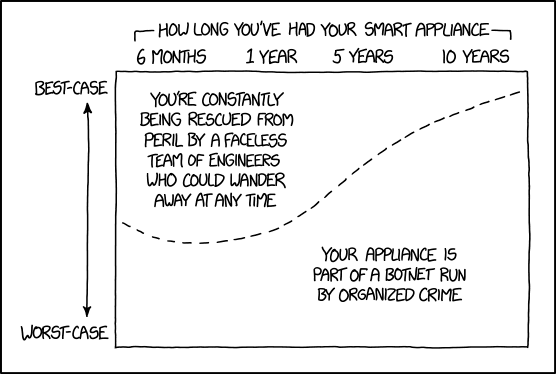
\includegraphics[width=0.7\textwidth,height=\textheight]{images/xkcd_1966_smart_home_security.png}

}

\caption{\href{https://xkcd.com/1966/}{xkcd: Smart Home Security},
cc-by-nc 2.5}

\end{figure}%

\section*{Aufbau}\label{aufbau}
\addcontentsline{toc}{section}{Aufbau}

\markright{Aufbau}

Das Skript führt in Sensorik ein und zeigt typische Anwendungen zum
Thema IoT, des Weiteren zeigt es auf wie Sensordaten genutzt,
gespeichert, übertragen und visualisiert werden können.

\begin{itemize}
\tightlist
\item
  Teil 1: Sensoren
\item
  Teil 2: Datenspeicherung
\item
  Teil 3: Datenkommunikation und Visualisierung
\end{itemize}

Die begleitenden Übungen nutzen den Einplatinenrechner Raspberry Pi mit
unterschiedlichen Sensoren für die Datenerfassung, -analyse und
Visualisierung. Die Programmiersprache für diesen Kurs ist Python und
das genutzte Betriebssystem ist Raspberry Pi OS, eine für den Raspberry
Pi angepasste Distribution von Debian (Linux).

\begin{boxtitle}{Hinweis}{colPrimary}

\textbf{Lernziele:}

\begin{itemize}
\tightlist
\item
  Die Studierenden erfahren, wie IoT (Internet of Things) und
  Sensordaten in räumlicher Analyse eingesetzt werden können.
\item
  Die Studierenden lernen, wie sie mit einem Einplatinenrechner
  Sensordaten erfassen, auswerten, kommunizieren und visualisieren
  können.
\end{itemize}

\end{boxtitle}

\section*{Kursvorbereitung}\label{kursvorbereitung}
\addcontentsline{toc}{section}{Kursvorbereitung}

\markright{Kursvorbereitung}

Für den Kurs werden Raspberry Pi 4 mit dem Breakout Garden HAT und
passenden Sensoren zur Verfügung gestellt. In den Computerräumen besteht
Zugang zu externen Bildschirmen, Tastatur und Mäusen, mit denen die
Übungen mit dem Raspberry Pi durchgeführt werden können.

\begin{figure}[H]

{\centering 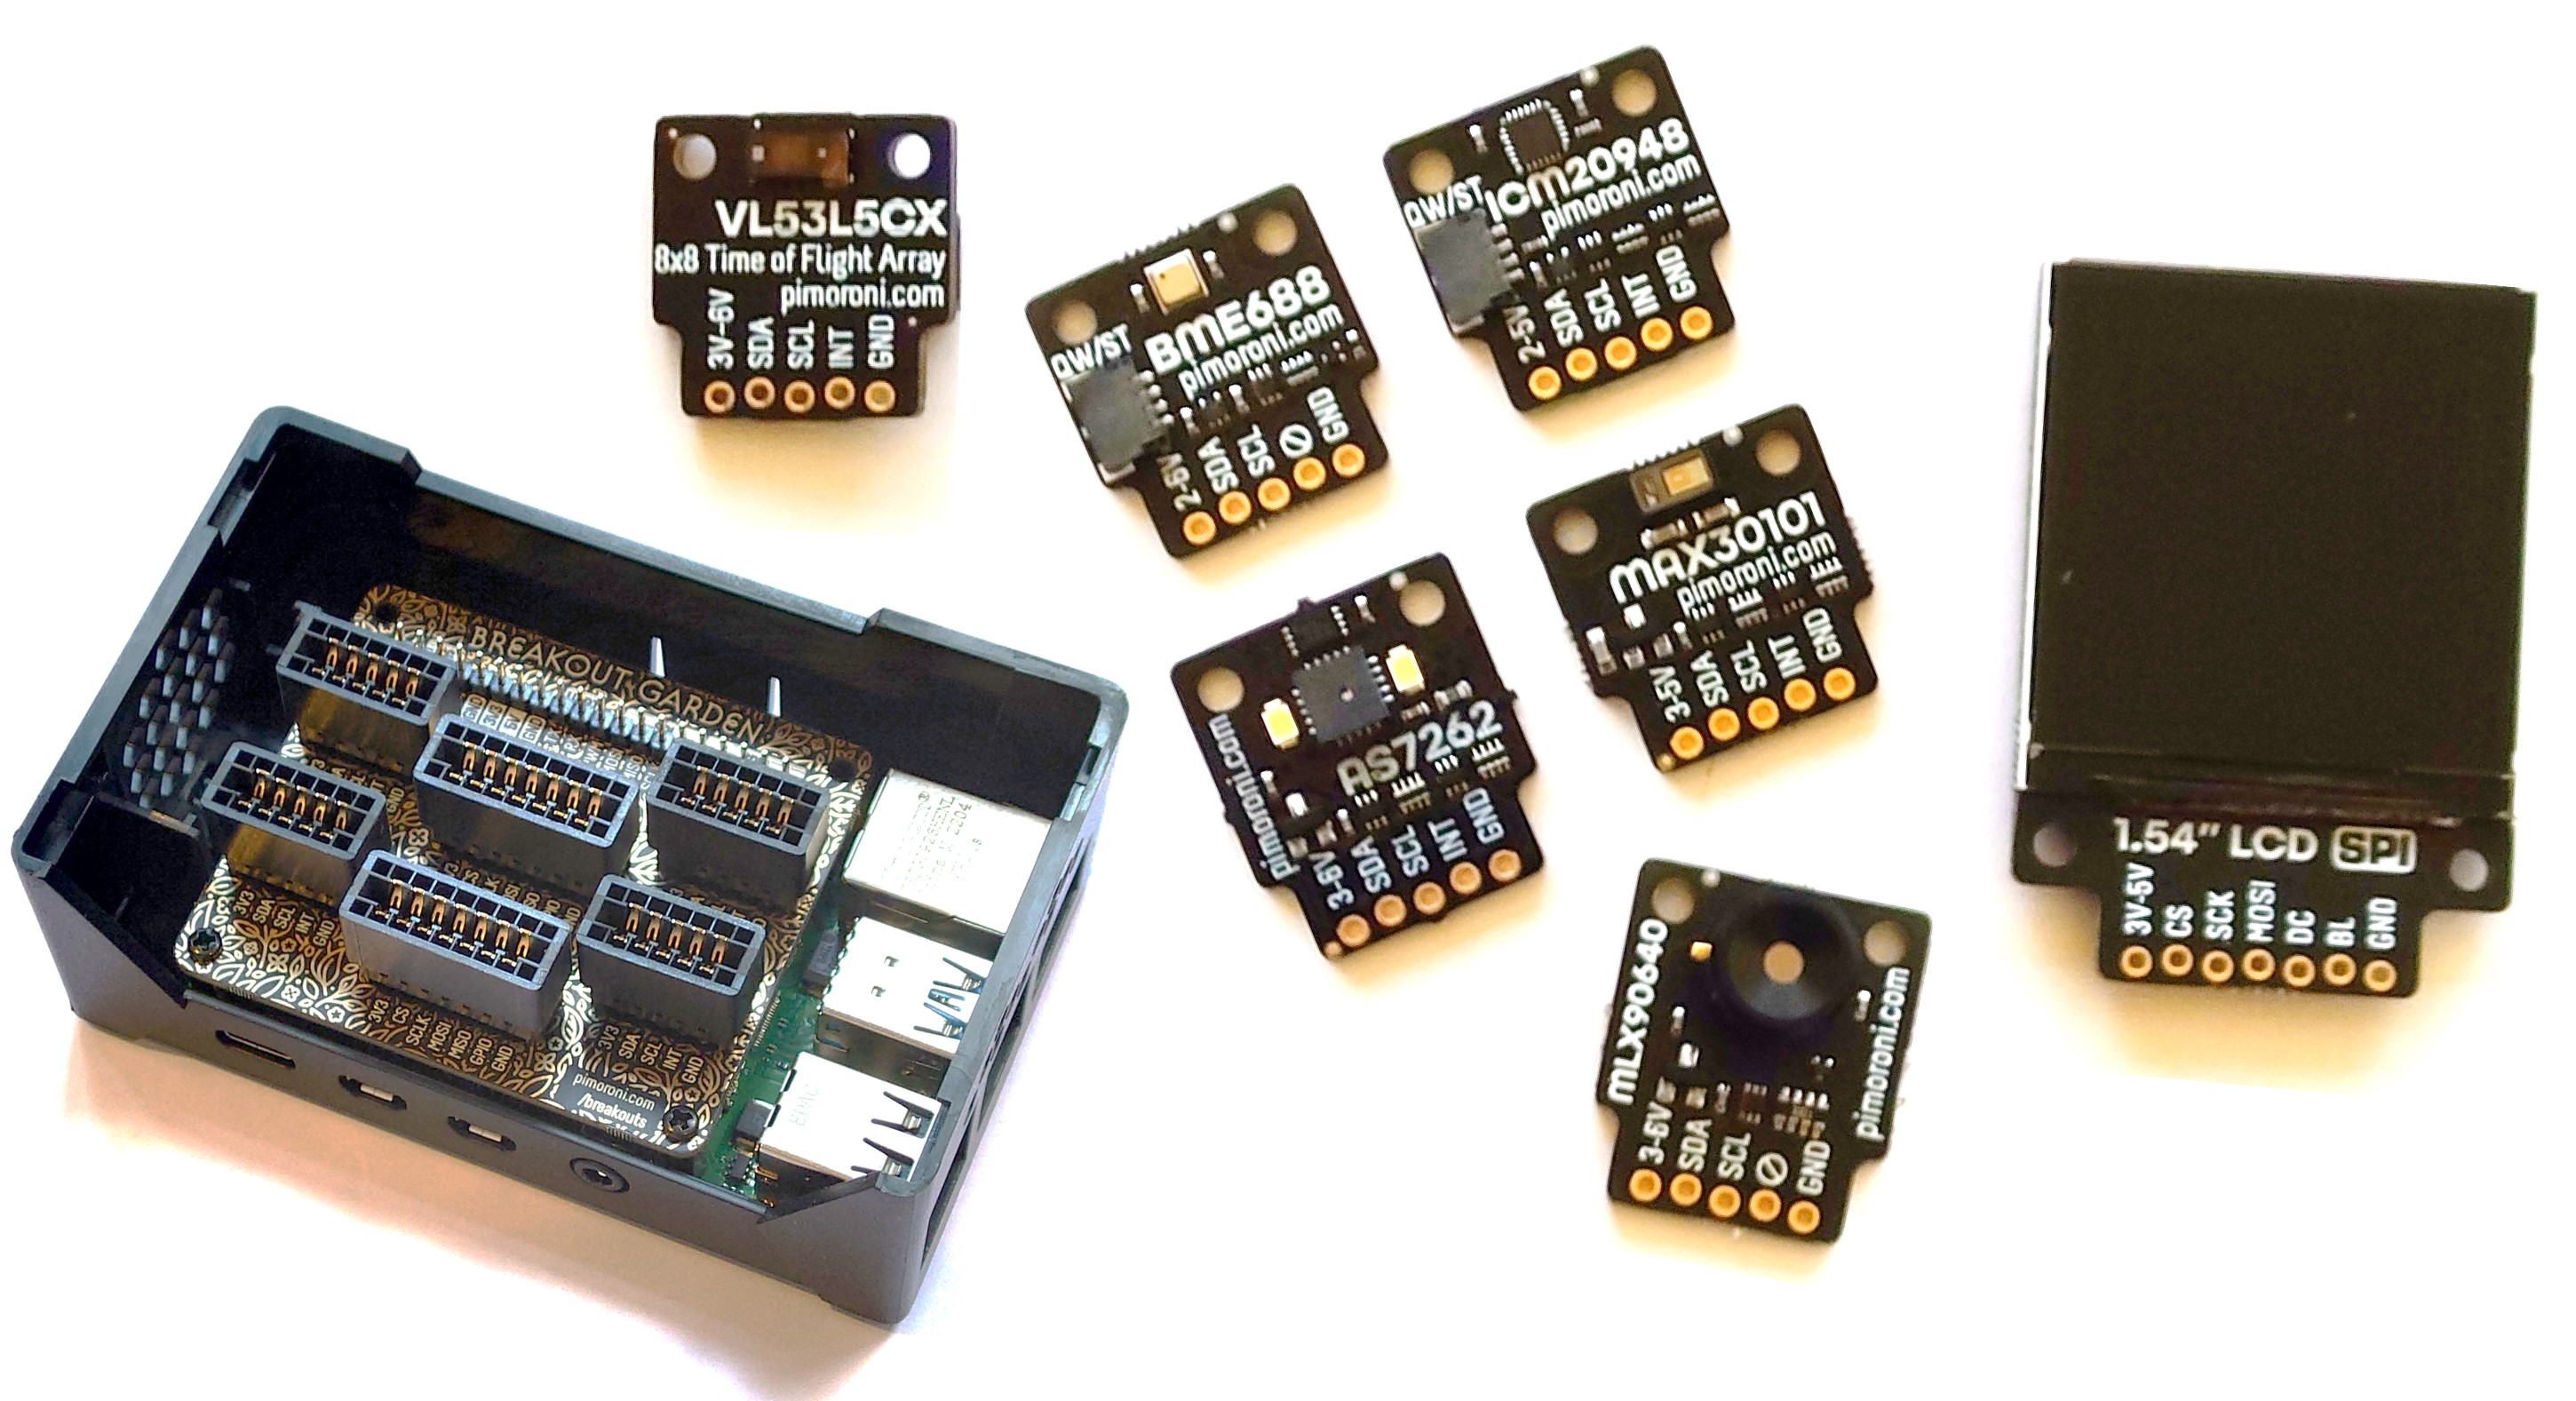
\includegraphics{images/raspberry_pi_set.jpg}

}

\caption{Raspberry Pi Set: Raspberry Pi 4 mit Breakout Garden HAT und
Sensoren}

\end{figure}%

Für den Fernzugriff auf den Raspberry Pi und entwickeln ist ein
SSH-Client (SSH Windows, Putty, Tabby), sowie eine entsprechende
Entwicklungsumgebung mit Python (Anaconda, Miniconda) und Visual Studio
Code empfohlen.

\begin{itemize}
\tightlist
\item
  SSH-Clients: \href{https://www.putty.org}{Putty},
  \href{https://tabby.sh/}{Tabby}
\item
  Python: \href{https://www.anaconda.com/download}{Anaconda},
  \href{https://docs.conda.io/projects/miniconda/en/latest/}{Miniconda},
  \href{https://www.python.org/}{Python}
\end{itemize}

\section*{Raspberry Pi Image
Einstellungen}\label{raspberry-pi-image-einstellungen}
\addcontentsline{toc}{section}{Raspberry Pi Image Einstellungen}

\markright{Raspberry Pi Image Einstellungen}

Für die Übungen wird ein Raspberry Pi Image mit vorinstallierten Paketen
und Einstellungen verwendet. Die SD-Karte mit dem Image wird von der
Kursleitung zur Verfügung gestellt. Das Image kann über Moodle bezogen
werden.

\begin{longtable}[]{@{}llll@{}}
\caption{Raspberry Pi Image Konto Einstellungen}\tabularnewline
\toprule\noalign{}
Konto & User & Passwort & Kommentar \\
\midrule\noalign{}
\endfirsthead
\toprule\noalign{}
Konto & User & Passwort & Kommentar \\
\midrule\noalign{}
\endhead
\bottomrule\noalign{}
\endlastfoot
Raspberry Pi & iot & \texttt{igeo@fhnw} & \\
influxdb & iot & \texttt{igeo@fhnw} & organisation: \texttt{fhnw} \\
grafana & admin & \texttt{igeo@fhnw} & \\
\end{longtable}

\section*{Übungsunterlagen}\label{uxfcbungsunterlagen}
\addcontentsline{toc}{section}{Übungsunterlagen}

\markright{Übungsunterlagen}

Die Übungsunterlagen werden auf dieser Kurswebseite Einführung in IoT
zur Verfügung gestellt und werden laufend aktualisiert.

\section*{Repository}\label{repository}
\addcontentsline{toc}{section}{Repository}

\markright{Repository}

Die Inhalte von ``Einführung in IoT'' sind auf der
\href{https://314a.github.io/5200_IoT}{Kurswebseite} frei zugänglich und
sind unter \href{https://creativecommons.org/licenses/by-nc/4.0/}{CC
BY-NC 4.0}'' lizenziert. Ideen, Änderungen und Vorschläge sind
willkommen und können über das
\href{https://github.com/314a/5200_IoT}{GitHub Repository} eingebracht
werden. Die Kurswebseite wird mit \href{https://quarto.org/}{Quarto}
erstellt.

\part{Theorie}

\chapter{Internet of Things IoT}\label{internet-of-things-iot}

Einführung in Internet of Things IoT und deren Bedeutung für die
Geomatik.

\hfill\break

\section{Ubiquitous Computing}\label{ubiquitous-computing}

Aus dem Bestreben der 1980er Jahre, Technologie in den Hintergrund des
Alltags einzubetten, in dem entstehenden Forschungsgebiet
\emph{Ubiquitous Computing} definierte dies Weiser \emph{Ubiquitous
Computing} (Rogers 2006) als ``die physische Welt, die reichhaltig und
unsichtbar mit Sensoren, Aktoren, Anzeigen und Computerelementen
verwoben ist, die nahtlos in die alltäglichen Objekte unseres Lebens
eingebettet und durch ein kontinuierliches Netzwerk verbunden ist'' mit
dem Ziel im täglichen Leben unterstützend zu sein und nicht zu
überladen.

\begin{description}
\item[Ubiquitous Computing\index{Ubiquitous Computing}]
Vision der Informatik allgegenwärtige Datenverarbeitung und Nutzung von
Systemen ohne Bedienungsanforderung und Hardwarebelastung für die
Nutzenden. Ubiquitäre Systeme agieren quasi unsichtbar im Hintergrund
von Handlungsfelder (Wiegerling 2013).
\end{description}

Ethnographische Studien über den Alltag zeigen, dass der Kontext des
Alltags der Menschen viel subtiler, fliessender und eigenwilliger ist,
als das die Theorien über den Kontext glauben machen (Salvador und
Anderson 2003). Dies erschwert eine praktische Umsetzung und Vorhersage
von Bedürfnissen auf Basis von Kontextinformationen erheblich.
Zusätzlich stellen sich auch ethische und soziale Fragen. Rogers (2006)
plädiert für einen proaktiven Ansatz weg von \emph{proactive Computing}
zu \emph{proactive people} und propagiert eine fachspezifische Nutzung
für bestimmte Bereiche wie beispielsweise Landwirtschaft oder
Umeltsanierung und weg von der Idee von \emph{pervasive Computing}. Zwei
Technologien sind kritisch für diese Ansätze \emph{Cloud Computing} und
\emph{Internet of Things}.

\section{Internet of Things}\label{internet-of-things}

Es existiert keine einheitliche Definition für \emph{Internet of Things}
IoT oder das Internet der Dinge. Es ist eine Bezeichnung oder
Sammelbegriff für ein Netzwerk von physischen Objekten ``Things'', die
untereinander vernetzt sind, mit Sensoren, Software und
unterschiedlichen Technologien ausgestattet sind, und somit einen
direkten Datenaustausch ermöglichen. Dies reicht von Monitoringsystemen,
über Wildtierbeobachtungen, Smart City Anwendungen bis in die Haushalte
die mit IoT Geräten ausgestattet sind.

Der Standardisierungsausschuss der International Telecommunication Union
(ITU) definiert IoT\index{IoT} als eine

\begin{quote}
.. a global~infrastructure~for the information society, enabling
advanced services by interconnecting~(physical and virtual)~Things based
on existing and evolving interoperable information and communication
technologies (ITU 2005).
\end{quote}

Ashton (2009) beschrieb als früher Ideengeber zu Internets der Dinge im
Kontext von Supply Chain Management folgendes:

\begin{quote}
.. Ideas and information are important, but things matter much more. Yet
today's information technology is so dependent on data originated by
people that our computers know more about ideas than things. If we had
computers that knew everything there was to know about things --- using
data they gathered without any help from us---we would be able to track
and count everything, and greatly reduce waste, loss and cost. We would
know when things needed replacing, repairing or recalling, and whether
they were fresh or past their best. We need to empower computers with
their own means of gathering information, so they can see, hear and
smell the world for themselves, in all its random glory. RFID and sensor
technology enable computers to observe, identify and understand the
world---without the limitations of human-entered data. {[}..{]} The
Internet of Things has the potential to change the world, just as the
Internet did. Maybe even more so.
\end{quote}

Die Kernidee von IoT ist, mit Computer Informationen, \emph{ohne}
menschliches zu tun zu erkennen. Wenn \emph{Dinge} eigenständig Daten
sammeln, diese nach Art, Messung, Messzeit und Messort geordnet werden,
ermöglicht dies im Bereich der Geomatik spannende neue Ansätze, Analysen
und Anwendungen. IoT ist ein multidisziplinäres Gebiet mit einem breiten
Spektrum an Technologien, Protokollen, Anwendungszenarien und
Disziplinen und bedingt Kenntnisse der elektronischen Komponenten,
Kommunikationsprotokollen, Echtzeitdatenanalysen, und der Lokalisierung
von Objekten und Geräten (Granell \emph{u.~a.} 2020).

Für das Konzept \emph{Ding} oder \emph{Thing} bestehen unterschiedliche
Definitionen. Charakteristisch ist, begrenzte Ressourcen (beispielsweise
geringe Rechenleistung), unzuverlässige Netwerkverbindung, geringe
Kosten für Hardware und Datenübertragung, keine Stromversorgung dafür
Batterienbetrieb und nicht im Office-Umfeld sondern im Feld. Aus
\textbf{Netzwerksicht} kann es als Entität mit der Möglichkeit sich mit
einem Netzwerk lokal oder dem Internet zu verbinden beschrieben werden.
Aus \textbf{\emph{ding-zentrierter} Sicht} sind die mit den Dingen
verbundenen Dienste zentral. Dienste, die Datenmengen, die von
intelligenten Objekten durch deren Interaktion mit der Umgebung erfasst
werden, verwalten.

\begin{figure}[H]

{\centering 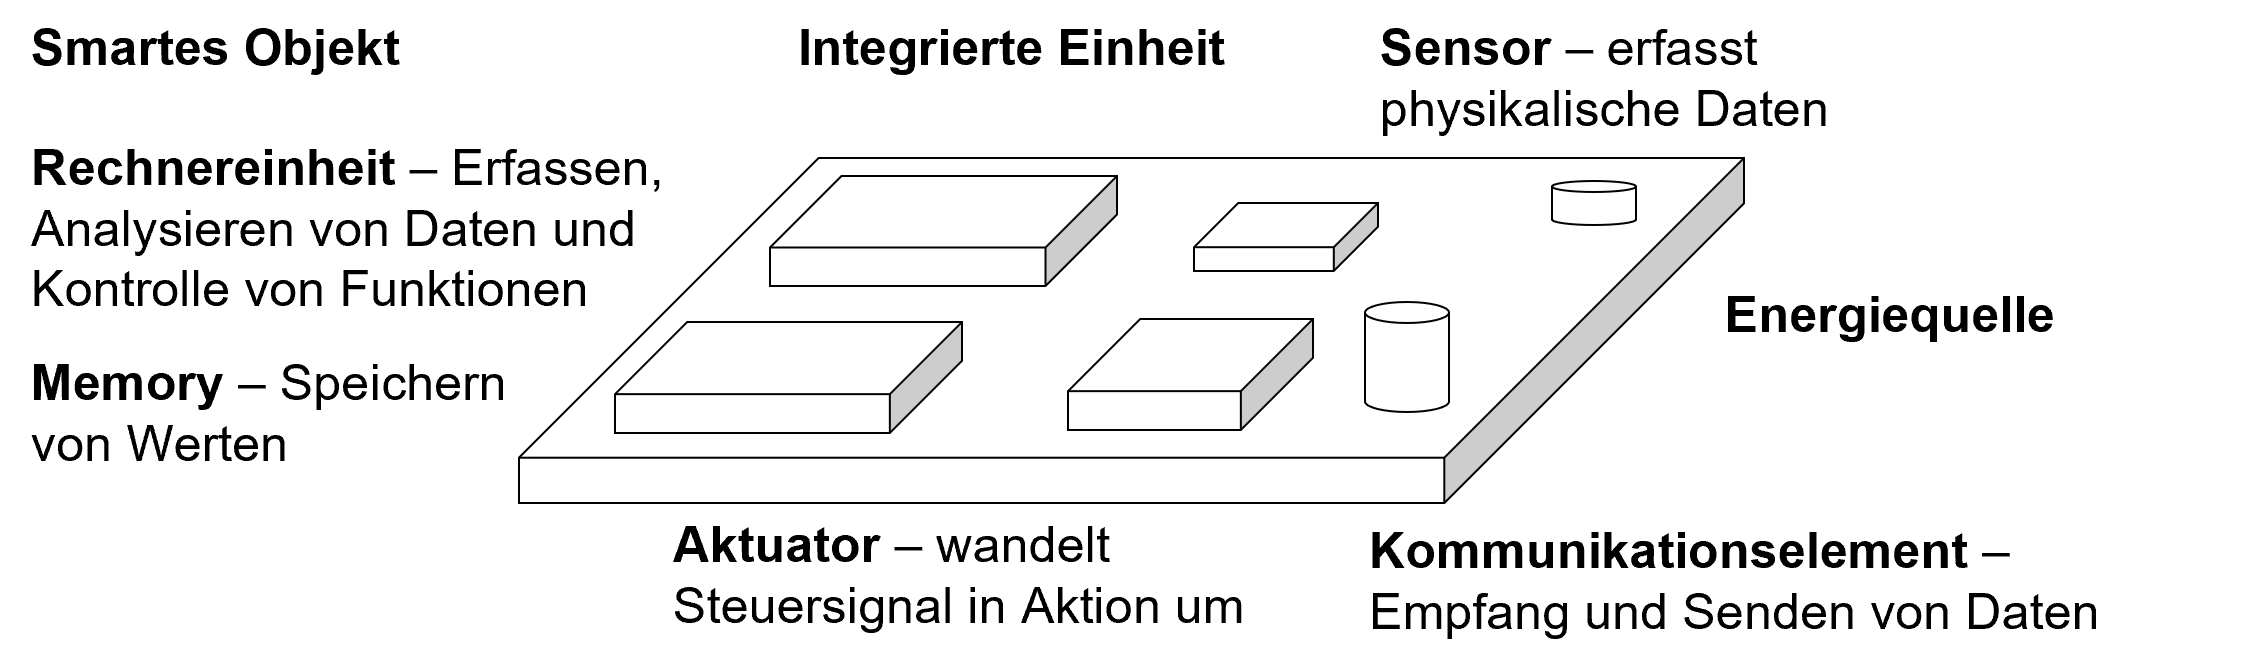
\includegraphics[width=0.8\textwidth,height=\textheight]{images/smartes_objekt.png}

}

\caption{Komponenten eines smarten Objekt ``Thing'' (Zaheeruddin und
Gupta 2020)}

\end{figure}%

Das Internet entwickelt sich in ein Netzwerk,

\begin{itemize}
\tightlist
\item
  in welchem Objekte miteinander \textbf{verbunden} werden,
\item
  Informationen aus der Umwelt gesammelt werden (\textbf{Sensorik}),
\item
  mit der physischen Welt interagiert (\textbf{Steuerung}) werden und
\item
  bestehende \textbf{Standards} für Dienste für den Transfer, Analyse,
  Anwendung und Kommunikation genutzt werden.
\end{itemize}

Die drei wesentlichen technologischen IoT Komponenten sind folglich:

\begin{itemize}
\tightlist
\item
  Hardware mit Sensoren, Aktoren und integrierter
  Kommunikationstechnologie
\item
  Middleware bedarfsorientierte Speicher- und
  Datenverarbeitungswerkzeuge für die Datenanalyse
\item
  Präsentation mit zugänglichen und nutzerfreundlichen Visualisierungs-
  und Interpretationswerkzeuge über unterschiedliche Plattformen und
  Anwendungen
\end{itemize}

Betrachtet man die Dimensionen von IoT fügt sich aus der Sicht der
Kommunikationstechnologie das \emph{thing} mit ein (ITU 2005). Aus Sicht
der Geoinformation, sind diese drei Dimensionen sehr vertraut mit
\emph{Zeit}, \emph{Ort} und \emph{Objekt} dem \emph{thing}.

\begin{figure}[H]

{\centering 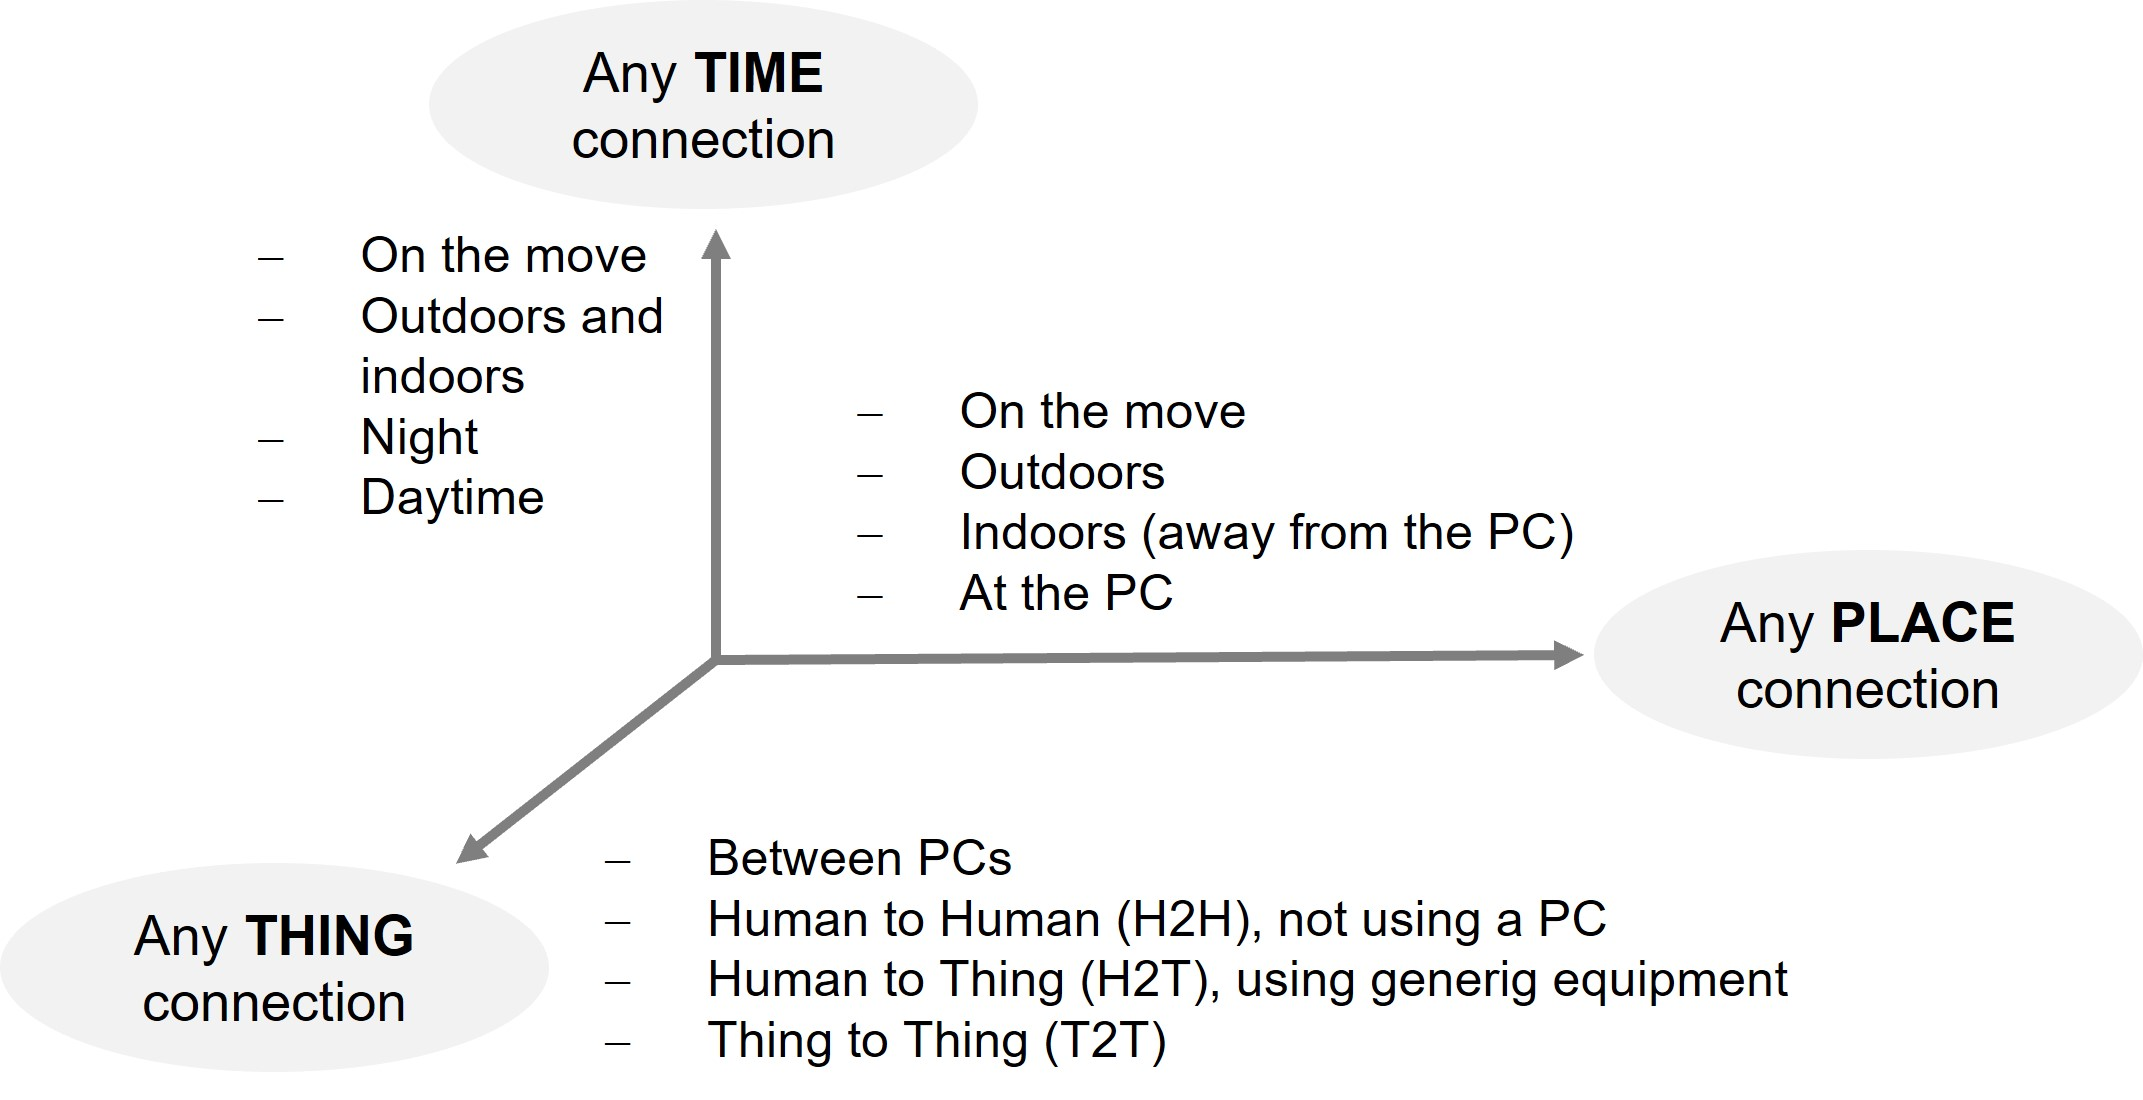
\includegraphics[width=0.8\textwidth,height=\textheight]{images/iot_dimension.jpg}

}

\caption{Dimensionen der IoT, eine neue Dimension aus Sicht der
Kommunikationstechnologie}

\end{figure}%

IoT Geräte haben neben der wichtigsten Eigenschaft, dass sie mit dem
Netzwerk/Internet kommunizieren können, folgende typischen
Eigenschaften. Sie sind oft \textbf{funkbasiert} und oft
\textbf{batteriebetrieben}. Sie lassen sich daher einfach installieren,
jedoch muss im Betrieb dem Batteriebetrieb der Verbrauch berücksichtigt
werden und nach Anforderung (Laufzeit vs häufige Updates) priorisiert
werden\footnote{Der Raspberry Pi ist insofern mit dem
  verhältnissmässigen hohen Stromverbrauch kein typisches IoT Device}.

\section{Digital Earth und IoT}\label{digital-earth-und-iot}

Der Vizepräsident der USA AL Gore führte 1998 in seiner Rede das Konzept
der digitalen Erde ein mit der Vision die realer Erde mit einer
virtuellen Nachbildung zu erweitern, einem virtuellen Zwilling (Gore
1998).

\begin{quote}
I believe we need a ``Digital Earth''. A multi-resolution,
three-dimensional representation of the planet into which we can embed
vast quantities of geo-referenced data. Gore (1998)
\end{quote}

Die Umsetzung der Vision ``Digital Earth''\index{Digital Earth}
erfordert wie auch die IoT eine entsprechende Infrastruktur, die das
Auffinden, den Zugriff, die Analyse und die Verarbeitung von
raumbezogenen Daten ermöglicht. Granell \emph{u.~a.} (2020) fordern eine
permanente und verstärkte Zusammenarbeit beider Bereiche. Betrachtet man
die Rolle der Netzwerke und Interaktion in beiden Bereichen, kann ein
Worklow von (1) der Auffindbarkeit, Erfassung und Kommunikation
räumlicher Informationen, zu (2) Verständnis räumlicher Objekte und
ihrer Beziehungen, dann (3) Bestimmung des raum-zeitlichen Verhaltens
und der Simulationsregeln und dem (4) Handeln und Ergreifen fundierter
Maßnahmen gezeichnet werden. Bei (1) kann IoT mit neuen Quellen und
höheren Aufnahme- und Übertragungsfrequenzen den Workflow anreichern und
(2) erfordert eine kontinuierliche vertiefte Zusammenarbeit beider
Infrastrukturen. Im Bereich IoT werden räumlichen Analysen wird aufgrund
der aufkommenden Edge-Fog-Cloud Paradigmen zunehmen.

\begin{figure}[H]

{\centering 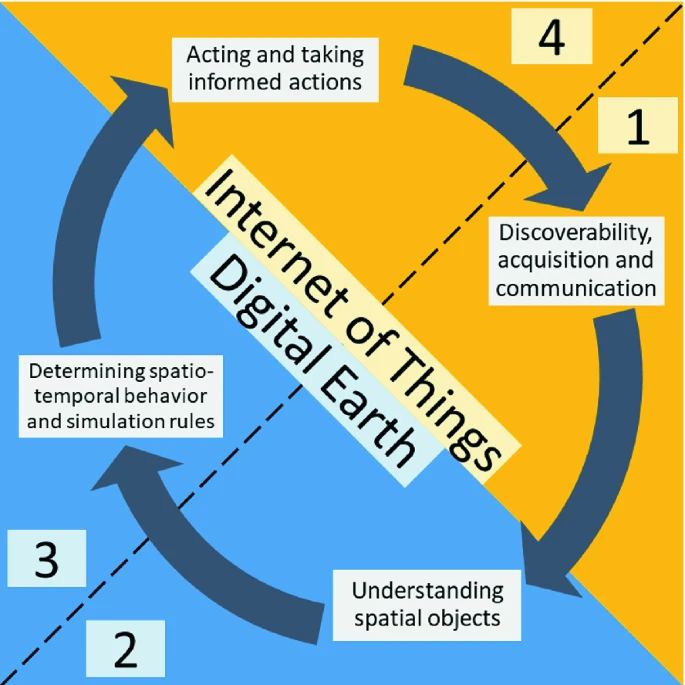
\includegraphics[width=0.5\textwidth,height=\textheight]{images/digital_earth_iot.png}

}

\caption{IoT und Digital Earth Workflow Granell \emph{u.~a.} (2020)}

\end{figure}%

\textbf{Die Auffindbarkeit, Erfassung und Kommunikation} räumlicher
Informationen erfordert das Geräte und ihre Daten auffindbar und
zugänglich sind mit standardisierten Methoden in globalen
zentralisierten Sammlungen, oder über dezentralen oder hierarchischen
Ansätzen. Viele dieser Dienste erfordern Fachkenntnisse und einfache
Zugänge zu IoT Daten fehlen. Der OGC Standard Sensor Web Enablement SWE
standardisiert die Erkennung und der Zugriff auf Sensoren. Bei der
räumlichen Datenerfassung in IoT haben Sensor-Metadaten eine hohe
Bedeutung, wobei der SensorML-Standard einer der wichtigsten ist
(Granell \emph{u.~a.} 2020).

\begin{description}
\tightlist
\item[Sensor Model Language SensorML-Standard\index{SensorML-Standard}]
Der OGC \href{https://www.ogc.org/standard/sensorml}{SensorML-Standard}
beschreibt umfassend Sensor-Metadaten und bietet eine Schnittstelle, die
das Auffinden von Sensoren und Beobachtungen folglich das Erstellen von
Suchindizes erleichtert. Elemente sind Betreiber, Dienste, Standort,
beobachtetes Phänomen und der zeitliche Verlauf.
\item[Sensor Web Enablement SWE standards
suite\index{Sensor Web Enablement SWE standards}]
Der OGC \href{https://www.ogc.org/standard/swes}{SWE Standard}
ermöglicht die Erkennung und den Zugriff auf Sensoren und zugehörige
Beobachtungsdaten über Standardprotokolle und
Anwendungsprogrammierschnittstellen. Anwendung in der Erdbeobachtung,
beispielsweise für das Katastrophenmanagement wie Brände,
Überschwemmungen oder Vulkanausbrüche. Wobei die Unterstützung der
Semantik eine Schwäche des Standards ist, \emph{Semantic Sensor Network
SSN} und Weiterentwicklungen wie \emph{Internet of Things Ontology
IoT-O} oder die \emph{Sensor, Observation, Sample, and Actuator (SOSA)
Ontology}, eine Zusammenarbeit zwischen W3C und OGC, nutzen Ontologien
um die Semantik in IoT besser abzubilden.
\end{description}

SWE umfasst zwei Suchtypen das Auffinden einzelner Sensorinstanzen und
Sensordienste, wobei ersteres sich auf einzelne Geräte oder
Sensornetzwerke bezieht und das Zweite die Dienste, die mit dem Sensor
interagieren. Die Suche kann grob in drei Gruppen unterteilt werden:

\begin{itemize}
\tightlist
\item
  \emph{thematisch}: Art der Phänomene, die ein Sensor beobachtet, z. B.
  Temperatur, Windstärke oder Luftdruck
\item
  \emph{räumlich}: Ort, an dem der Sensor eingesetzt wird
\item
  \emph{zeitlich}: Zeitraum, in dem die Beobachtungen gemacht werden
\end{itemize}

Weiterentwicklungen im Bereich der Kommunikation zwischen \emph{things}
Geräten brachte neue Schnittstellen und über die Zeit geringere Kosten
und Stromverbrauch der Kommunikationsschnittstellen wie \emph{Bluetooth,
Wi-Fi, ZigBee, 3G-5G} oder \emph{LORA}. Während früher einfache
Datenlogger nur Daten senden konnten verfügen die Geräte heute über die
Möglichkeit Daten zu Senden und zu empfangen. Dies erlaubt die Steuerung
und Anpassung des Verhaltens der Geräte. Kommunikationsprotokolle die
auf Maschinenkommunikation ausgerichtet sind \emph{machine-to-machine
M2M} wurden entwickelt, wie das \emph{Advanced Message Queuing
Protokoll} (AMQP), \emph{MQTT} oder das \emph{streamingorientierte
Protokoll STOMP}. Folgende Übersicht zeigt unterschiedliche
Eigenschaften von Industriestandards für IoT über die
Übertragungsdistanz, Art der Informationsübertragung und typische
Anwendungsbereiche.

\begin{figure}[H]

{\centering 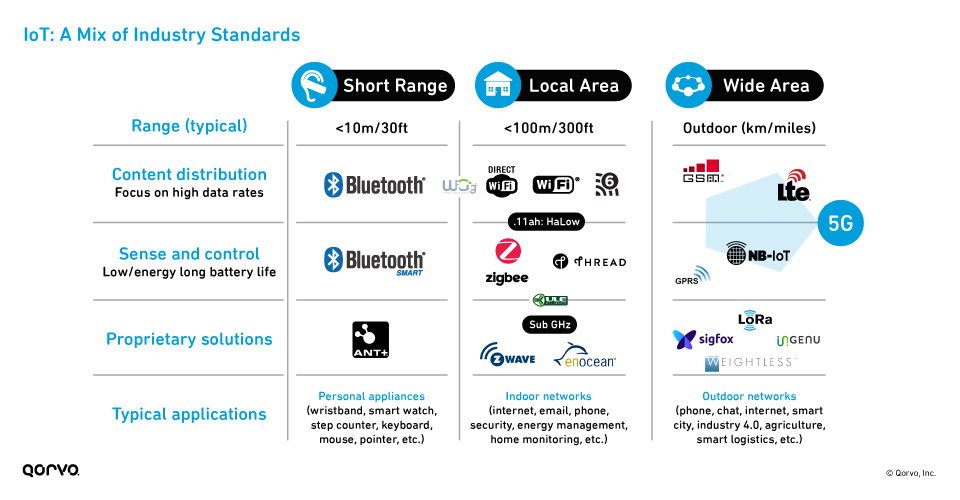
\includegraphics{images/iot_standards_range.png}

}

\caption{IoT Standards, Eigenschaften, Übertragungsdistanzen und
Anwendungen (Links 2019)}

\end{figure}%

\section{IoT und GIS}\label{iot-und-gis}

\emph{Smarte} Geräte der erzeugen grosse Datenströme mit zeitlichen und
räumlichen Merkmalen, für deren Analyse die Entfernung, Fläche, Volumen
oder Trajektorien entscheidend für die Datenanalyse von IoT Geräten
sind. Die Vielfalt der Geräte bringt neue analytische Herausforderungen
mit sich, die in der Lage sein müssen räumlich-zeitliche Echtzeitdaten
mit sehr heterogenen \emph{smarten} Geräten verarbeiten zu können
(Trilles \emph{u.~a.} 2017). Während Werkzeuge für die Analyse von
Echtzeitdaten existieren, stellt die räumliche Komponente eine
Herausforderung dar. Der Raum, wie der Standort, die Ausrichtung, Form
und Grösse spielen eine wesentliche Rolle in IoT, da alle Geräte
räumliche Eigenschaften aufweisen und miteinander räumlich zu einander
in Beziehung stehen (beispielsweise der Standort, die Grösse und
Orientierung von einem Auto und einem Fahrrad auf der gleichen Fahrbahn)
(Granell \emph{u.~a.} 2020). Erst über den Raum können Sensoren in
Beziehung zu einander gebracht werden.

Ansätze zur räumlichen-zeitlichen Datenanalyse in Echtzeit haben noch
keine standardisierten Prozeduren, die einfach und breit angewandt
werden können (Granell \emph{u.~a.} 2020). Zusätzlich sollten Standards
Echtzeitanalysen ermöglichen ohne grossen zusätzlichen Rechenaufwand für
Geräte, die eine beschränkte \emph{Speicherkapazität} und
\emph{Konnektivität} haben und oft mit Batterie betrieben sind. Der OGC
Sensor Observation Service SOS bedingt eine eher rechenintensive
Verarbeitung von XML-Dokumenten und weitere Ansätze sind in Erarbeitung,
die dem Rechnung tragen.

Kamilaris und Ostermann (2018) klassieren und geben eine Übersicht von
IoT Anwendungen\index{IoT Anwendungen} und Forschungsprojekte im Kontext
der GIScience und IoT. Die Anwendungsbiete sind vielfältig, wie in
folgender Abbildung illustriert. In fast allen aufgeführten
Anwendungsgebieten sind Aussagen zum Standort relevant.

\begin{figure}[H]

{\centering 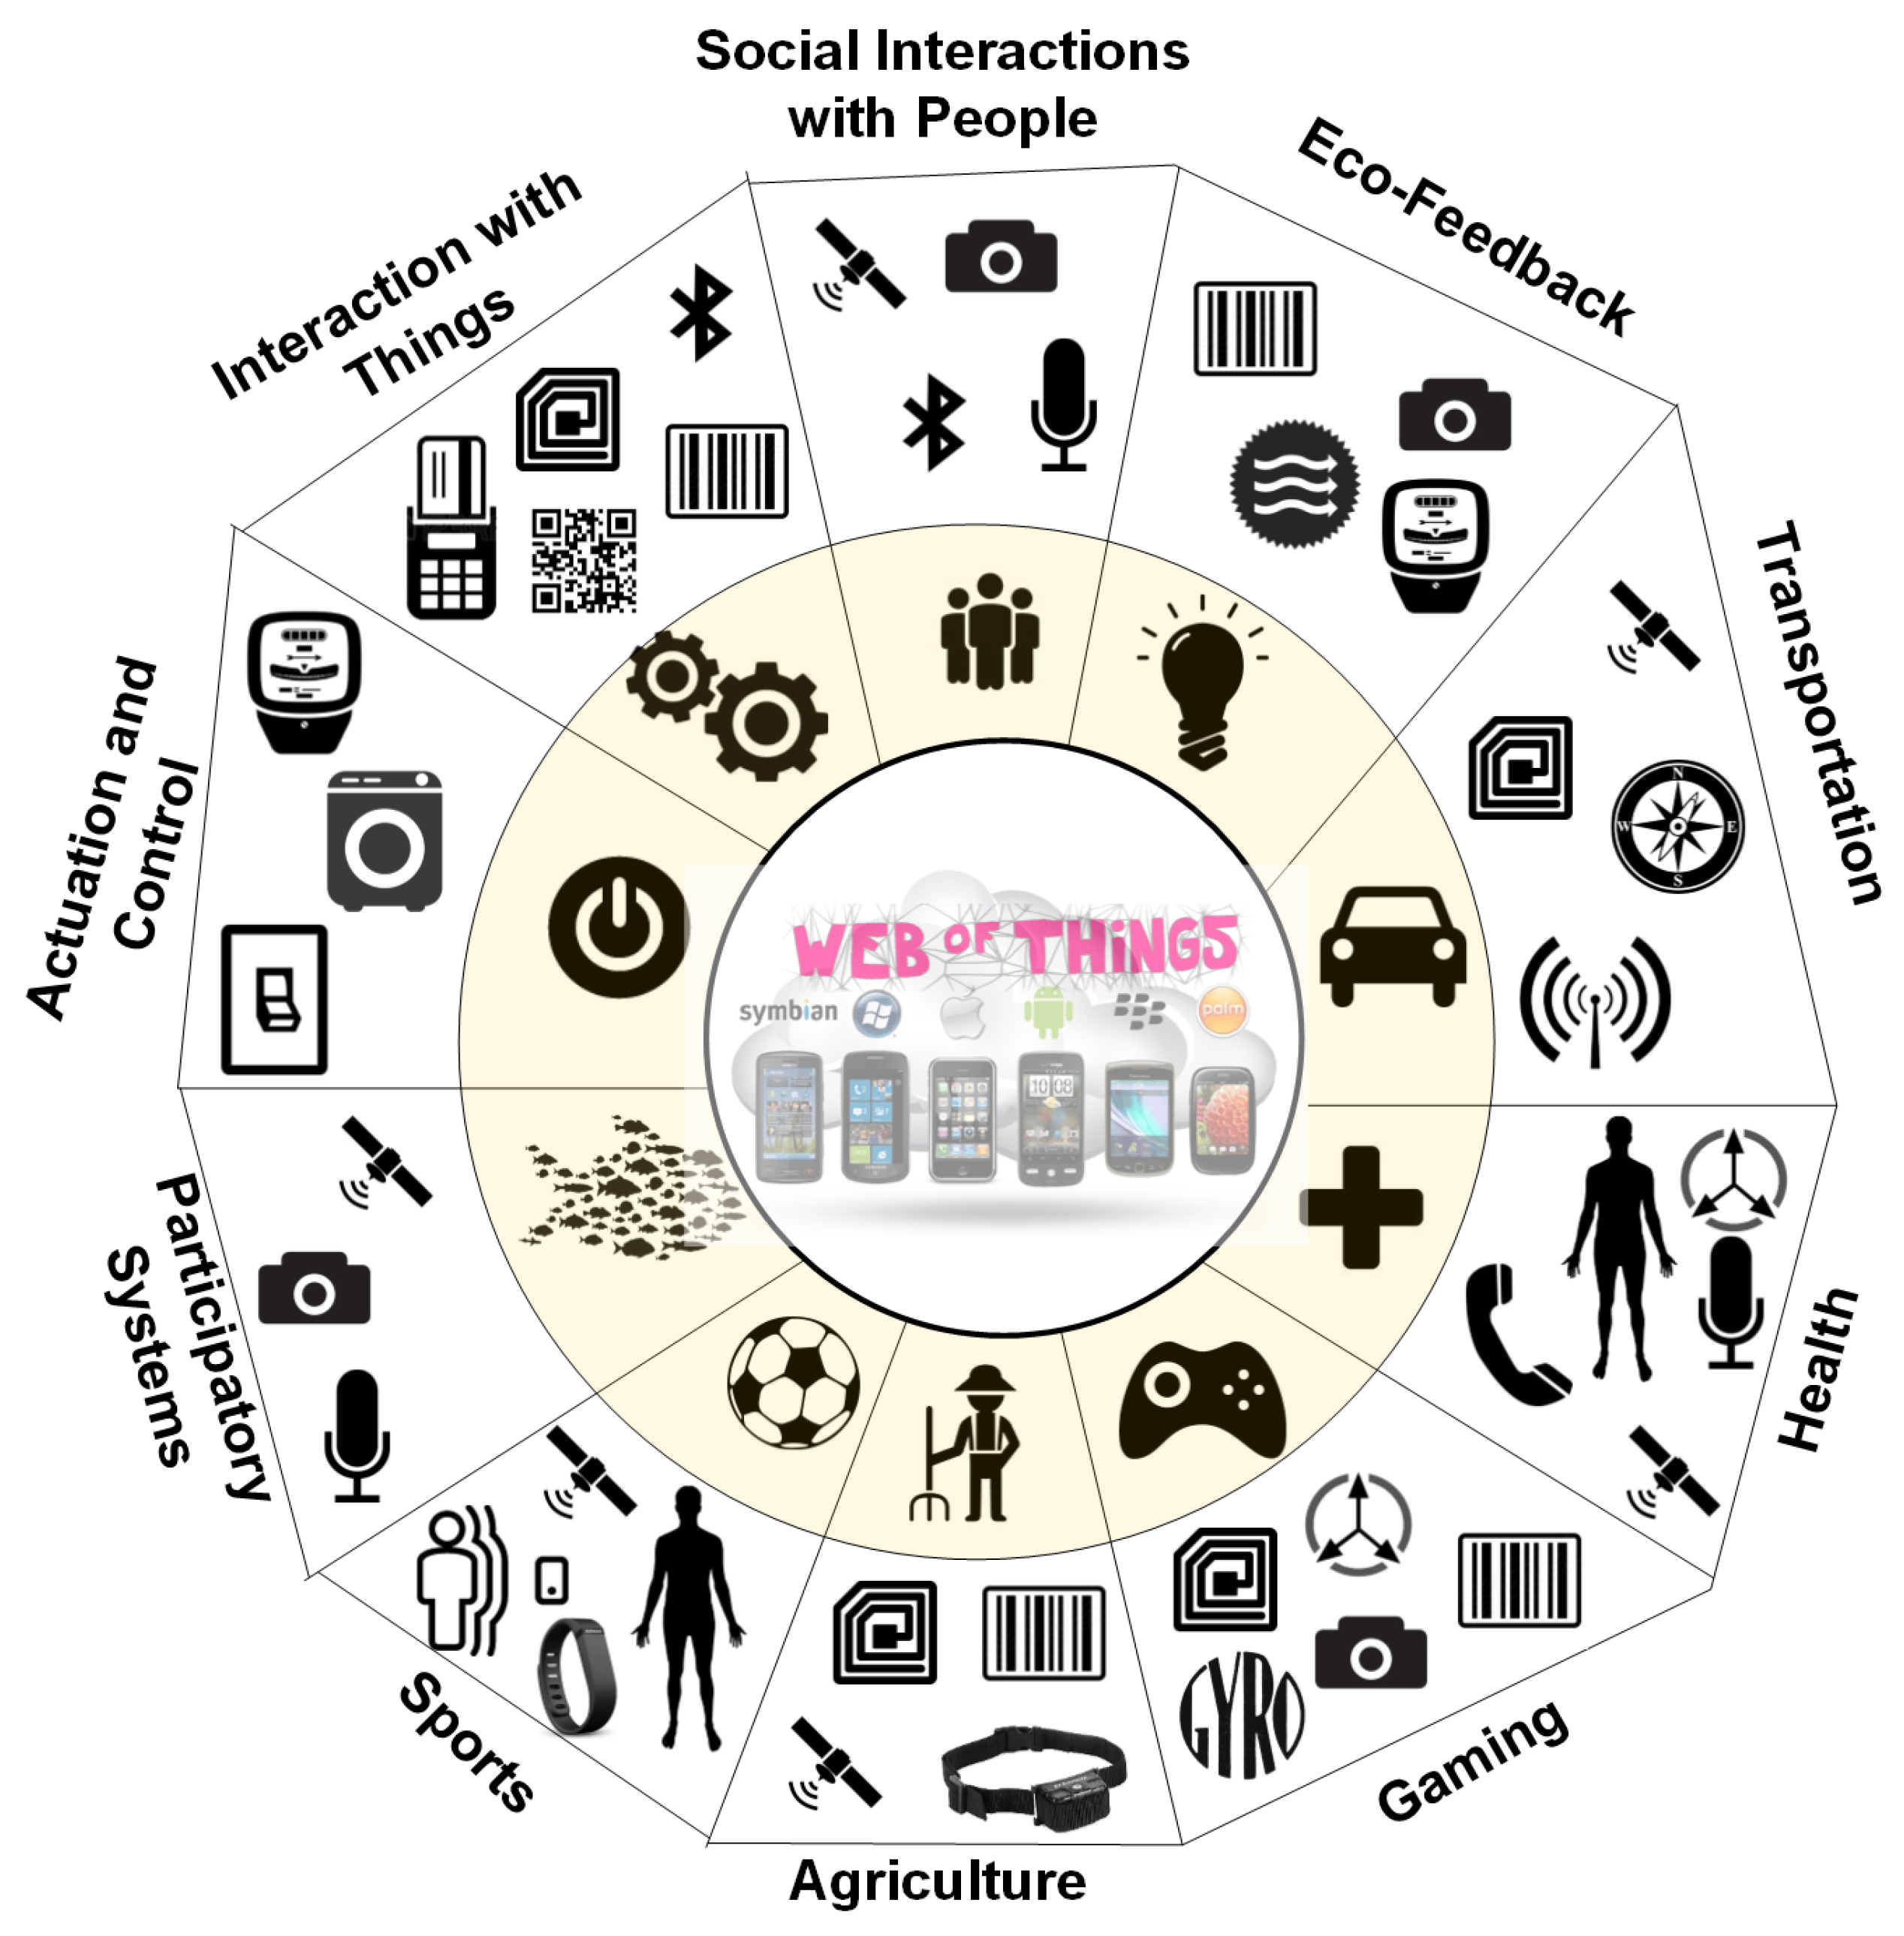
\includegraphics[width=0.5\textwidth,height=\textheight]{images/iot_ecosystem_mobile.png}

}

\caption{Ökosystem der Anwendungen in mobile Computing im Zusammenspiel
mit Sensoren von IoT Geräten.}

\end{figure}%

Sie führen für die verschiedenen Anwendungsgebiete die benutzten
Methodenklassen der räumlichen Analyse\index{Räumliche Analysemethoden}.

Wobei sie die Analysemethoden wie folgt gruppieren:

\begin{itemize}
\tightlist
\item
  \textbf{Geometric Measures}: distances and proximity of points,
  adjacency and connectivity
\item
  \textbf{Data Mining}: discovering patterns from large datasets
\item
  \textbf{Basic Analytical Operations}: methods such as buffering and
  overlay
\item
  \textbf{Basic Analytical Methods}: spatial analysis of point patterns
  and clusters, kernels and density analysis
\item
  \textbf{Network Analysis}: graph measures, least-cost shortest path
  problems and flow modeling
\item
  \textbf{Surface Analysis \& Geostatistics}: Analysis of surfaces and
  geostatistics deal with interpolation of surfaces and kriging.
\end{itemize}

Sie klassieren die Anwendungsgebiete und die räumlichen Analysemethoden
in folgender Tabelle.

\begin{longtable}[]{@{}
  >{\raggedright\arraybackslash}p{(\columnwidth - 12\tabcolsep) * \real{0.1795}}
  >{\raggedright\arraybackslash}p{(\columnwidth - 12\tabcolsep) * \real{0.1154}}
  >{\raggedright\arraybackslash}p{(\columnwidth - 12\tabcolsep) * \real{0.0705}}
  >{\raggedright\arraybackslash}p{(\columnwidth - 12\tabcolsep) * \real{0.1731}}
  >{\raggedright\arraybackslash}p{(\columnwidth - 12\tabcolsep) * \real{0.1538}}
  >{\raggedright\arraybackslash}p{(\columnwidth - 12\tabcolsep) * \real{0.1026}}
  >{\raggedright\arraybackslash}p{(\columnwidth - 12\tabcolsep) * \real{0.2051}}@{}}
\caption{IoT Forschungsgebiet und räumliche Analysemethoden (Kamilaris
und Ostermann 2018).}\tabularnewline
\toprule\noalign{}
\begin{minipage}[b]{\linewidth}\raggedright
IoT Area
\end{minipage} & \begin{minipage}[b]{\linewidth}\raggedright
Geometric Measures
\end{minipage} & \begin{minipage}[b]{\linewidth}\raggedright
Data Mining
\end{minipage} & \begin{minipage}[b]{\linewidth}\raggedright
Basic Analytical Operations
\end{minipage} & \begin{minipage}[b]{\linewidth}\raggedright
Basic Analytical Methods
\end{minipage} & \begin{minipage}[b]{\linewidth}\raggedright
Network Analysis
\end{minipage} & \begin{minipage}[b]{\linewidth}\raggedright
Surface Analysis \& Geostatistics
\end{minipage} \\
\midrule\noalign{}
\endfirsthead
\toprule\noalign{}
\begin{minipage}[b]{\linewidth}\raggedright
IoT Area
\end{minipage} & \begin{minipage}[b]{\linewidth}\raggedright
Geometric Measures
\end{minipage} & \begin{minipage}[b]{\linewidth}\raggedright
Data Mining
\end{minipage} & \begin{minipage}[b]{\linewidth}\raggedright
Basic Analytical Operations
\end{minipage} & \begin{minipage}[b]{\linewidth}\raggedright
Basic Analytical Methods
\end{minipage} & \begin{minipage}[b]{\linewidth}\raggedright
Network Analysis
\end{minipage} & \begin{minipage}[b]{\linewidth}\raggedright
Surface Analysis \& Geostatistics
\end{minipage} \\
\midrule\noalign{}
\endhead
\bottomrule\noalign{}
\endlastfoot
Tourism & X & X & - & X & - & - \\
Utility Network & X & X & - & - & X & - \\
Disaster Monitoring & X & - & X & - & - & X \\
Health and disease detection & X & X & - & X & - & X \\
Transportation & X & X & - & X & X & - \\
Logistics and assets & - & X & - & - & X & - \\
Wildlife monitoring & - & X & - & X & X & X \\
Agriculture & X & - & - & X & X & X \\
Crime prediction & - & - & - & X & - & - \\
Sports and gaming & X & - & - & X & - & - \\
Environment & - & - & X & X & X & X \\
\end{longtable}

In einer zweiten tabellarischen Zusammenfassung führen sie IoT basierte
Methoden mit Beispielen von Generalisierung von Punktmessungen auf,
welche Aussagen in grösseren Massstäben ermöglichen. Diese sind nach
einzelnen IoT Methoden klassiert, wobei die ersten vier Methoden gerade
für Generalisierung\index{Generalisierung von Messdaten} am beliebtesten
sind.

\begin{longtable}[]{@{}
  >{\raggedright\arraybackslash}p{(\columnwidth - 2\tabcolsep) * \real{0.2762}}
  >{\raggedright\arraybackslash}p{(\columnwidth - 2\tabcolsep) * \real{0.7238}}@{}}
\caption{IoT Methoden für die Generalisierung von Analysen (Kamilaris
und Ostermann 2018).}\tabularnewline
\toprule\noalign{}
\begin{minipage}[b]{\linewidth}\raggedright
IoT-Based Method
\end{minipage} & \begin{minipage}[b]{\linewidth}\raggedright
Examples of Generalizations
\end{minipage} \\
\midrule\noalign{}
\endfirsthead
\toprule\noalign{}
\begin{minipage}[b]{\linewidth}\raggedright
IoT-Based Method
\end{minipage} & \begin{minipage}[b]{\linewidth}\raggedright
Examples of Generalizations
\end{minipage} \\
\midrule\noalign{}
\endhead
\bottomrule\noalign{}
\endlastfoot
Participatory sensing & Detecting emergency events at city scale
{[}\href{https://www.mdpi.com/2220-9964/7/7/269\#B23-ijgi-07-00269}{1}{]},
promoting neighborhood identity and local services
{[}\href{https://www.mdpi.com/2220-9964/7/7/269\#B24-ijgi-07-00269}{2}{]},
creating a noise map of a city
{[}\href{https://www.mdpi.com/2220-9964/7/7/269\#B25-ijgi-07-00269}{3}{]},
detecting outbreaks of dengue fever
{[}\href{https://www.mdpi.com/2220-9964/7/7/269\#B48-ijgi-07-00269}{4}{]},
developing heat maps from cyclists used for better city planning
{[}\href{https://www.mdpi.com/2220-9964/7/7/269\#B45-ijgi-07-00269}{5}{]},
producing a global spatial distribution of malaria risk
{[}\href{https://www.mdpi.com/2220-9964/7/7/269\#B65-ijgi-07-00269}{6}{]}. \\
Vehicular networks and transportation systems & Proactively performing
urban traffic monitoring
{[}\href{https://www.mdpi.com/2220-9964/7/7/269\#B54-ijgi-07-00269}{7}{]},
travel planning based on real-time traffic information
{[}\href{https://www.mdpi.com/2220-9964/7/7/269\#B12-ijgi-07-00269}{8}{]}. \\
Fixed IoT sensors & Urban decision-making assistance
{[}\href{https://www.mdpi.com/2220-9964/7/7/269\#B13-ijgi-07-00269}{9}{]},
wildlife monitoring and understanding of herd behavior
{[}\href{https://www.mdpi.com/2220-9964/7/7/269\#B60-ijgi-07-00269}{10}{]},
monitoring the area levels of air pollution
{[}\href{https://www.mdpi.com/2220-9964/7/7/269\#B46-ijgi-07-00269}{11}{]},
creating air temperature and precipitation maps
{[}\href{https://www.mdpi.com/2220-9964/7/7/269\#B70-ijgi-07-00269}{12}{]},
understanding fish-school characteristics around artificial reefs
{[}\href{https://www.mdpi.com/2220-9964/7/7/269\#B67-ijgi-07-00269}{13}{]},
estimating the level variations of the sand layer of sandy beaches or
dunes
{[}\href{https://www.mdpi.com/2220-9964/7/7/269\#B66-ijgi-07-00269}{14}{]}. \\
Satellite imagery & Understanding how invasive species respond to
landscape configuration relative to native species
{[}\href{https://www.mdpi.com/2220-9964/7/7/269\#B49-ijgi-07-00269}{15}{]},
assessing how the livestock agriculture affects the physical environment
{[}\href{https://www.mdpi.com/2220-9964/7/7/269\#B35-ijgi-07-00269}{16},\href{https://www.mdpi.com/2220-9964/7/7/269\#B50-ijgi-07-00269}{17}{]},
modeling forest fire risk zones
{[}\href{https://www.mdpi.com/2220-9964/7/7/269\#B33-ijgi-07-00269}{18}{]},
earthquake risk assessment
{[}\href{https://www.mdpi.com/2220-9964/7/7/269\#B34-ijgi-07-00269}{19}{]},
planning of tsunami evacuation
{[}\href{https://www.mdpi.com/2220-9964/7/7/269\#B36-ijgi-07-00269}{20}{]},
creating digital maps with information about bacteria habitats
{[}\href{https://www.mdpi.com/2220-9964/7/7/269\#B47-ijgi-07-00269}{21}{]},
delineating groundwater potential zones in hard rock terrain
{[}\href{https://www.mdpi.com/2220-9964/7/7/269\#B39-ijgi-07-00269}{22}{]}. \\
Ground sensor sampling & Estimating the Grand Canyon height map
{[}\href{https://www.mdpi.com/2220-9964/7/7/269\#B63-ijgi-07-00269}{23}{]},
generating high-risk floodplain maps
{[}\href{https://www.mdpi.com/2220-9964/7/7/269\#B63-ijgi-07-00269}{24}{]},
creating soil fertility maps
{[}\href{https://www.mdpi.com/2220-9964/7/7/269\#B72-ijgi-07-00269}{25}{]},
assessing the spatial variation of groundwater quality and producing
salinity hazard maps
{[}\href{https://www.mdpi.com/2220-9964/7/7/269\#B69-ijgi-07-00269}{26}{]},
assessing the heavy metal pollution in soils
{[}\href{https://www.mdpi.com/2220-9964/7/7/269\#B71-ijgi-07-00269}{27}{]},
estimating the zinc contamination concentrations around a lake
{[}\href{https://www.mdpi.com/2220-9964/7/7/269\#B68-ijgi-07-00269}{28}{]}. \\
Web-based IoT datasets & Estimating traffic from historical traffic
flows
{[}\href{https://www.mdpi.com/2220-9964/7/7/269\#B42-ijgi-07-00269}{29}{]},
optimizing routes of public transportation based on taxi rides
{[}\href{https://www.mdpi.com/2220-9964/7/7/269\#B43-ijgi-07-00269}{30}{]},
exploring and analyzing attractive areas
{[}\href{https://www.mdpi.com/2220-9964/7/7/269\#B38-ijgi-07-00269}{31}{]},
associating assault rates to measures of population and place
characteristics
{[}\href{https://www.mdpi.com/2220-9964/7/7/269\#B41-ijgi-07-00269}{32}{]}. \\
Combination of IoT methods & Assessing damage in Haiti by earthquake and
facilitating emergency response
{[}\href{https://www.mdpi.com/2220-9964/7/7/269\#B61-ijgi-07-00269}{33}{]},
infrastructure asset management
{[}\href{https://www.mdpi.com/2220-9964/7/7/269\#B58-ijgi-07-00269}{34}{]}. \\
\end{longtable}

\chapter{Sensoren}\label{sensoren}

\section{Sensoren in IoT}\label{sensoren-in-iot}

Einer der grossen Treiber von IoT ist die zuhnemende Verfügbarkeit von
low-cost Sensoren für viele unterschiedliche Anwendungen. Standard
Sensoren sind beispielweise Umweltsensoren wie Temperatur,
Luftfeuchtigkeit, Luftdruck, Bewegungssensoren mit Beschleunigung, und
Magnetfeld, Neigung, Standort Sensoren wie GPS oder Kamera Licht,
Schall, Gas, Flüssigkeit, wie auch Gesundheitssensoren wie
Herzfrequenzvariabilität sowie GSR (galvanische Hautreaktion oder
Hautleitfähigkeit). Sensoren sind in der Regel mit einem Mikrocontroller
verbunden, der die Messwerte verarbeitet und an einen Computer oder ein
anderes Gerät überträgt.

Der Trend geht hin zu Miniaturisierung und Multi-Sensor-Geräten mit dem
Vorteil, dass über mehrere Sensoren zeitgleich(!) Messungen durchgeführt
werden können und so aus der Kombination von Messwerten über
Sensordatenfusion (sensor fusion)\index{Sensor Fusion} neue Erkenntnisse
gewonnen werden können, beispielsweise die Kombination von GPS und
Beschleunigungssensor für die Bestimmung der Position und der
Geschwindigkeit (Dead Reckoning, Kalman Filter).

Sensoren können in mehrere Kategorien gruppiert werden:
Umweltüberwachung (natürliche und anthropogene), Biophysikalische
Sensoren und Gesundheitsüberwachung, Gebäude- und Heimautomatisierung,
Automobil- und Transportanwendungen, Mobile Computing und tragbare
Elektronik etc.

Viele Sensoren sind in Smartphones integriert, wie z.B.
Beschleunigungssensoren, Gyroskope, Magnetometer, GPS, Lichtsensoren,
Näherungssensoren, Barometer, Temperatursensoren, Feuchtigkeitssensoren,
Mikrofone, Kameras, etc. Ihr Einsatz ist vielfältig, von der
Unterhaltung über die Navigation bis hin zur Gesundheitsüberwachung. Mit
der Applikation \emph{\href{https://phyphox.org}{phyphox}\index{phyphox}
- physical phone experiments} einer digitalien Experimentierbox,
entwickelt von der RWTH Aachen University, können die Sensoren von
Smartphones für physikalische Experimente genutzt werden.

\begin{figure}[H]

{\centering 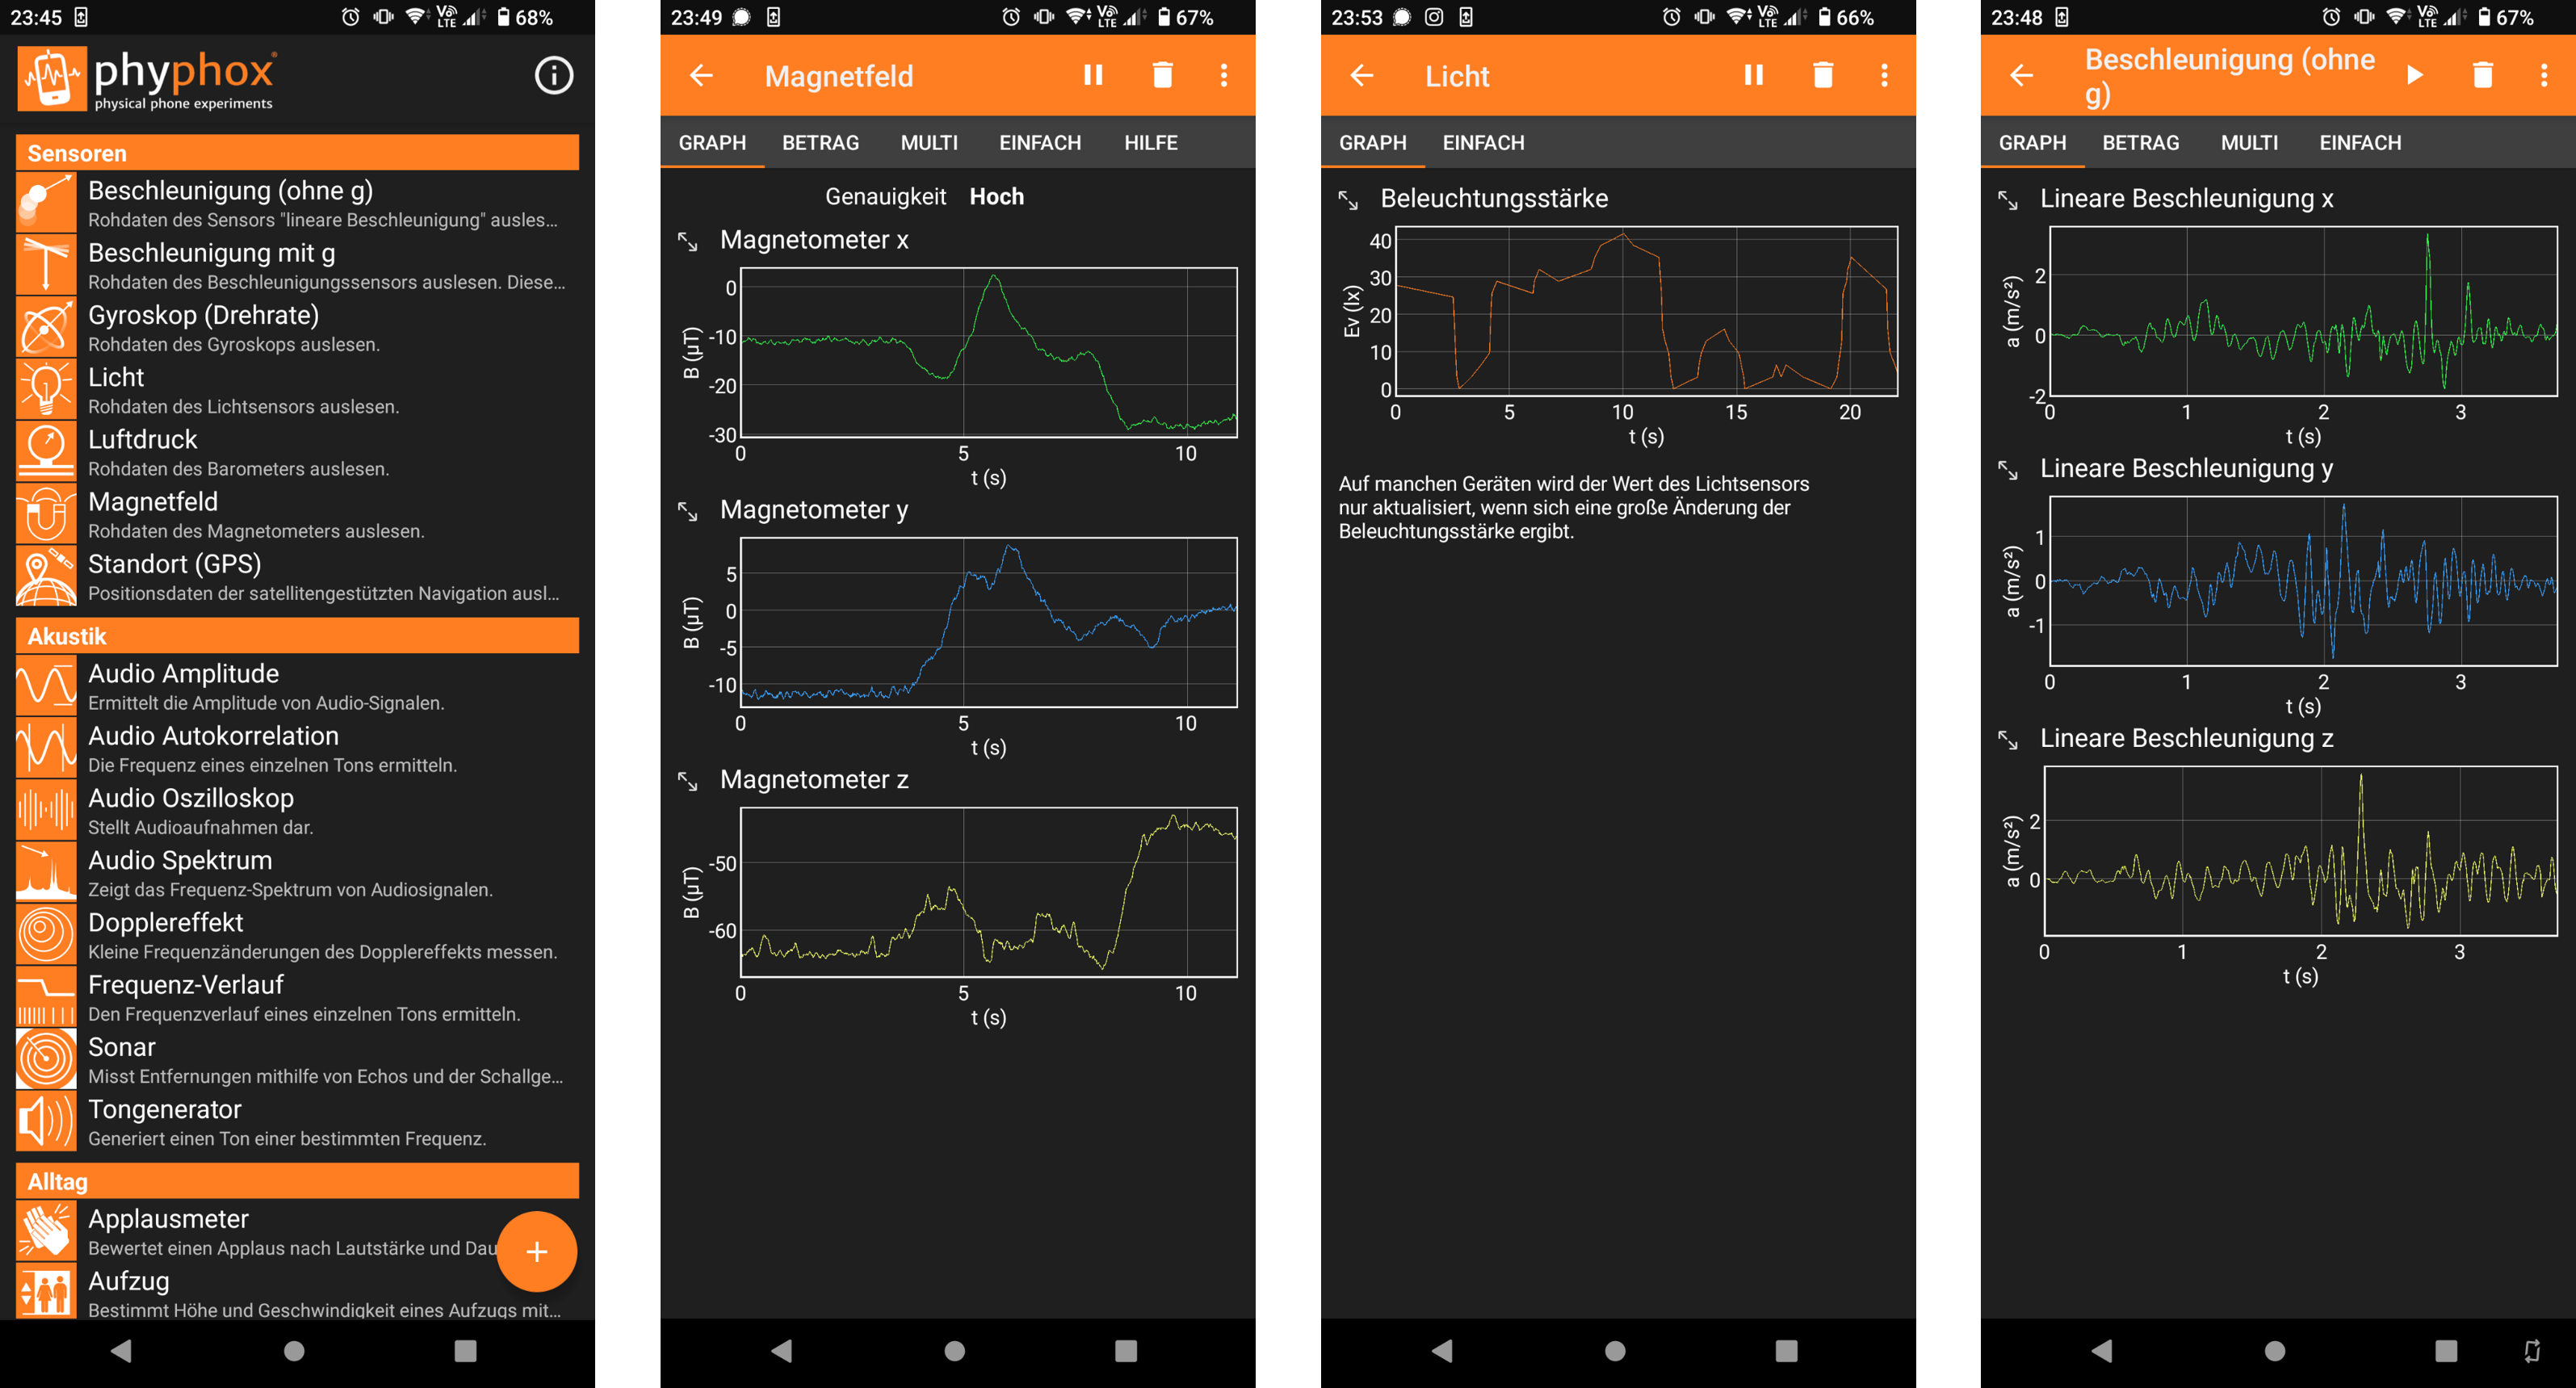
\includegraphics{images/phyphox.png}

}

\caption{phyphox Anwendung für physikalische Experimente mit Sensoren in
Mobiletelefonen, Screenshot der Anwendung mit dem Menu und einzelnen
Experimenten am Beispiel von Magnetfeld, Licht und Beschleunigung.}

\end{figure}%

\begin{boxtitle}{Excercise}{colPrimary}

\textbf{Sensorentest mit \emph{phyphox}}\\
Installiere auf deinem Smartphone die Applikation
\emph{\href{https://phyphox.org}{phyphox}} und teste die Sensoren deines
Smartphones, wie die Beschleunigung, Orientierung (Magnetfeld), Standort
oder Licht. Führe ein Experiment durch und dokumentiere deine
Beobachtungen. Nutze die Anwendung für Vergleiche mit anderen Sensoren
während der Übungen.

\end{boxtitle}

\section{Sensoren}\label{sensoren-1}

Sensoren\index{Sensoren} sind technische Bauteile, die bestimmte
physikalische oder chemische Eigenschaften messen oder eine
Beschaffenheit der Umgebung qualitativ oder quantitativ erfasst.
Sensoren können unterschiedlich klassiert werden, nach der Art der
Erzeugung von Energie in passive und aktive Sensoren, nach dem
Messprinzip oder dem Verwendungszweck.

\begin{longtable}[]{@{}
  >{\raggedright\arraybackslash}p{(\columnwidth - 2\tabcolsep) * \real{0.2105}}
  >{\raggedright\arraybackslash}p{(\columnwidth - 2\tabcolsep) * \real{0.7895}}@{}}
\caption{Wirkprinzip von Sensoren Quelle:
\href{https://de.wikipedia.org/wiki/Sensor}{wikipedia}}\tabularnewline
\toprule\noalign{}
\begin{minipage}[b]{\linewidth}\raggedright
Wirkprinzip
\end{minipage} & \begin{minipage}[b]{\linewidth}\raggedright
Beispiel
\end{minipage} \\
\midrule\noalign{}
\endfirsthead
\toprule\noalign{}
\begin{minipage}[b]{\linewidth}\raggedright
Wirkprinzip
\end{minipage} & \begin{minipage}[b]{\linewidth}\raggedright
Beispiel
\end{minipage} \\
\midrule\noalign{}
\endhead
\bottomrule\noalign{}
\endlastfoot
Mechanisch & Manometer, Dehnungshebel, Federwaage, Hebelwaage,
Thermometer \\
Thermoelektrisch & Thermoelement \\
Resistiv & Dehnungsmessungsstreifen, Hitzdraht, Halbleiter-DMS, Pt100 \\
Piezoelektrisch & Beschleunigungssensor \\
Kapazitiv & Drucksensor, Regensensor, Luftfeuchtesensor \\
Induktiv & Neigungssensor, Kraftsensor, Wegaufnehmer \\
Optisch & CCD-Sensor, Fotozelle \\
Akustisch & Füllstandssensor, Doppelbogenkontrolle,
Ultraschall-Durchflussmesser \\
Magnetisch & Hall-Sensoren, Reed-Kontakt \\
\end{longtable}

Die Wahl von Sensoren für IoT Projekte hängt von der Anwendung ab und
der dahinterstehenden Fragestellung. Die Fragestellung führt zur
Bestimmung was gemessen wird und wie das was gemessen werden soll
operationalisiert wird. Die Operationalisierung definiert die
Messgrössen und der Wahl von einem oder mehreren Sensoren (Sensor
Fusion) in einem IoT Projekt. Bei der Wahl sind mehrere Faktoren zu
berücksichtigen, wie beispielsweise:

\begin{itemize}
\tightlist
\item
  Welche Messgrösse soll gemessen werden? Welche Genauigkeit ist
  erforderlich? Welche Einschränkungen gibt es?
\item
  Existiert ein Datenblatt mit den technischen Spezifikationen?\\
\item
  Wie wird der Sensor angeschlossen? Wie wird der Sensor angesteuert?\\
\item
  Gibt es eine Einschränkung bezüglich der Temperatur und anderen
  Faktoren wie Feuchtigkeit?
\item
  Wie genau ist die Messung und welche Messabweichungen gibt es?
\item
  Existiert es eine Library, welche die Ansteuerung des Sensors
  vereinfacht? Gibt es einfache Beispiele, welche die Ansteuerung des
  Sensors zeigen? etc.
\end{itemize}

Für die Auswahl von Sensoren sind unter anderem folgende Aspekte zu
beachten:

\begin{itemize}
\tightlist
\item
  Anwendung (z.B. Umweltüberwachung, Gesundheitsüberwachung, Gebäude-
  und Heimautomatisierung, Automobil- und Transportanwendungen, Mobile
  Computing und tragbare Elektronik)
\item
  Messgrösse (z.B. Temperatur, Luftfeuchtigkeit, Luftdruck, Bewegung,
  Standort, Licht, Schall, Gas etc.) und Kombination von Messgrössen
  (Sensor Fusion)
\item
  Messprinzip (z.B. mechanisch, thermoelektrisch, resistiv,
  piezoelektrisch, kapazitiv, induktiv, optisch, akustisch, magnetisch)
\item
  Einschränkungen (z.B. Temperatur, Abschirmung)
\item
  Messgenauigkeit (z.B. Auflösung, Messbereich)
\item
  Bibliotheken (z.B. Programmiersprache, Dokumentation, Community,
  Beispiele, Aktualität)
\item
  Montage (Schnittstelle, Löten, HAT)
\item
  Datenschnittstelle (I2C, UART)
\item
  Platzbedarf
\item
  Stromversorgung (z.B. Batterie, Solarzelle, USB)
\item
  Kosten
\item
  Verfügbarkeit (z.B. Lagerbestand, Lieferzeit)
\item
  etc.
\end{itemize}

Für Prototypenentwicklung können über verschiedene Hersteller und
Distributoren Sensoren bezogen werden. Die folgende Liste gibt eine
Übersicht über einige Hersteller und Distributoren von Sensoren.

\begin{itemize}
\tightlist
\item
  \href{https://www.pi-shop.ch}{Pi-Shop} ist ein Schweizer Online
  Händler für Raspberry Pi und Zubehör.
\item
  \href{https://www.distrelec.ch}{Distrilec} ist ein Distributor für
  elektronische Bauteile in der Schweiz und Europa.
\item
  \href{https://www.adafruit.com}{Adafruit Industries} (2005, New York,
  USA) ist ein Hersteller von Elektronik für Maker gegründet von der
  MIT-Ingenieurin Limor ``Ladyada'' Fried.
\item
  \href{https://www.sparkfun.com}{Sparkfun Electronics} (2003, Colorado,
  USA) ist Open Source Elektronik Hersteller und produziert und verkauft
  Mikrocontroller-Plattformen, Sensoren und andere
  Elektronik-Komponenten.
\item
  \href{https://www.seeedstudio.com}{Seeed Technology} (2008, Shenzhen,
  China) ist eine IoT-Innovationsplattform das sich auf
  Hardware-Forschung, -Produktion und -Vertrieb für Edge-Computing,
  Netzwerkkommunikation und Smart-Sensing-Anwendungen spezialisiert hat
  und viele Produkte für Maker anbietet.
\item
  \href{https://shop.pimoroni.com}{Pimoroni} 2012 ist ein Reseller von
  Raspberry Pi, Adafruit, Micro:bit, Arduino, Sparkfun, etc. Produkten
  und stellt auch eigene Elektronikprodukte und Kits her\footnote{Trivia:
    Pimoroni steht für Pirate, Monkey, Robot, Ninja.}.
\end{itemize}

\begin{boxtitle}{Excercise}{colPrimary}

\textbf{Sensoren}\\
Suche Dir auf den aufgelisteten Websites für elektronische Bauteile und
Kits, wie dem Raspberry Pi, welche Art von Sensoren existieren. Suche
drei bis vier interessante Sensoren aus und überlege anhand der
aufgeführten Aspekte zur Sensorauswahl, was alles benötigt wird um diese
zu betreiben und was die Einschränkungen sind.

\end{boxtitle}

\chapter{Datenübertragung}\label{datenuxfcbertragung}

Drahtlose Kommunikationstechnologien basieren heutzutage auf IEEE
802.15.4 sowie IEEE 802.15.4e Übertragungsprotokoll (Celebi \emph{u.~a.}
2020). Das Protokoll beschreibt den die untersten beiden Schichten des
OSI Modells (Abbildung~\ref{fig-osimodell}), die Bitübertragung und den
MAC-Layer für Wireless Personal Area Networks (WPAN).

Einige der relevanten Technologien für die Datenübertragung sind, Wi-Fi,
Bluetooth, ZigBee, LoRa, RFID, SigFox und Mobilfunk. Die Technologien
unterscheiden sich in der Reichweite, der Datenrate, der
Energieeffizienz und der Anzahl der Geräte, die angeschlossen werden
können. Die Wahl der Technologie hängt von der Anwendung ab. Für die
Übertragung von Sensordaten über kurze Distanzen eignet sich Bluetooth,
ZigBee oder WiFi. Für die Übertragung von Sensordaten über lange
Distanzen eignet sich LoRa oder Mobilfunk. Für die Übertragung von
Sensordaten über kurze Distanzen mit hoher Datenrate eignet sich Wi-Fi.
Für die Übertragung von Sensordaten über kurze Distanzen mit geringer
Datenrate eignet sich RFID.

Je nach Anwendungsfall (Use Case) sind die Werte für die Latenzzeit
(Latency), Verlässlichkeit (Reliability), Größe der Datenmenge (Data
size), Reichweite (Range) für die Wahl der Kommunikationstechnologie
relevant.

\begin{figure}

\centering{

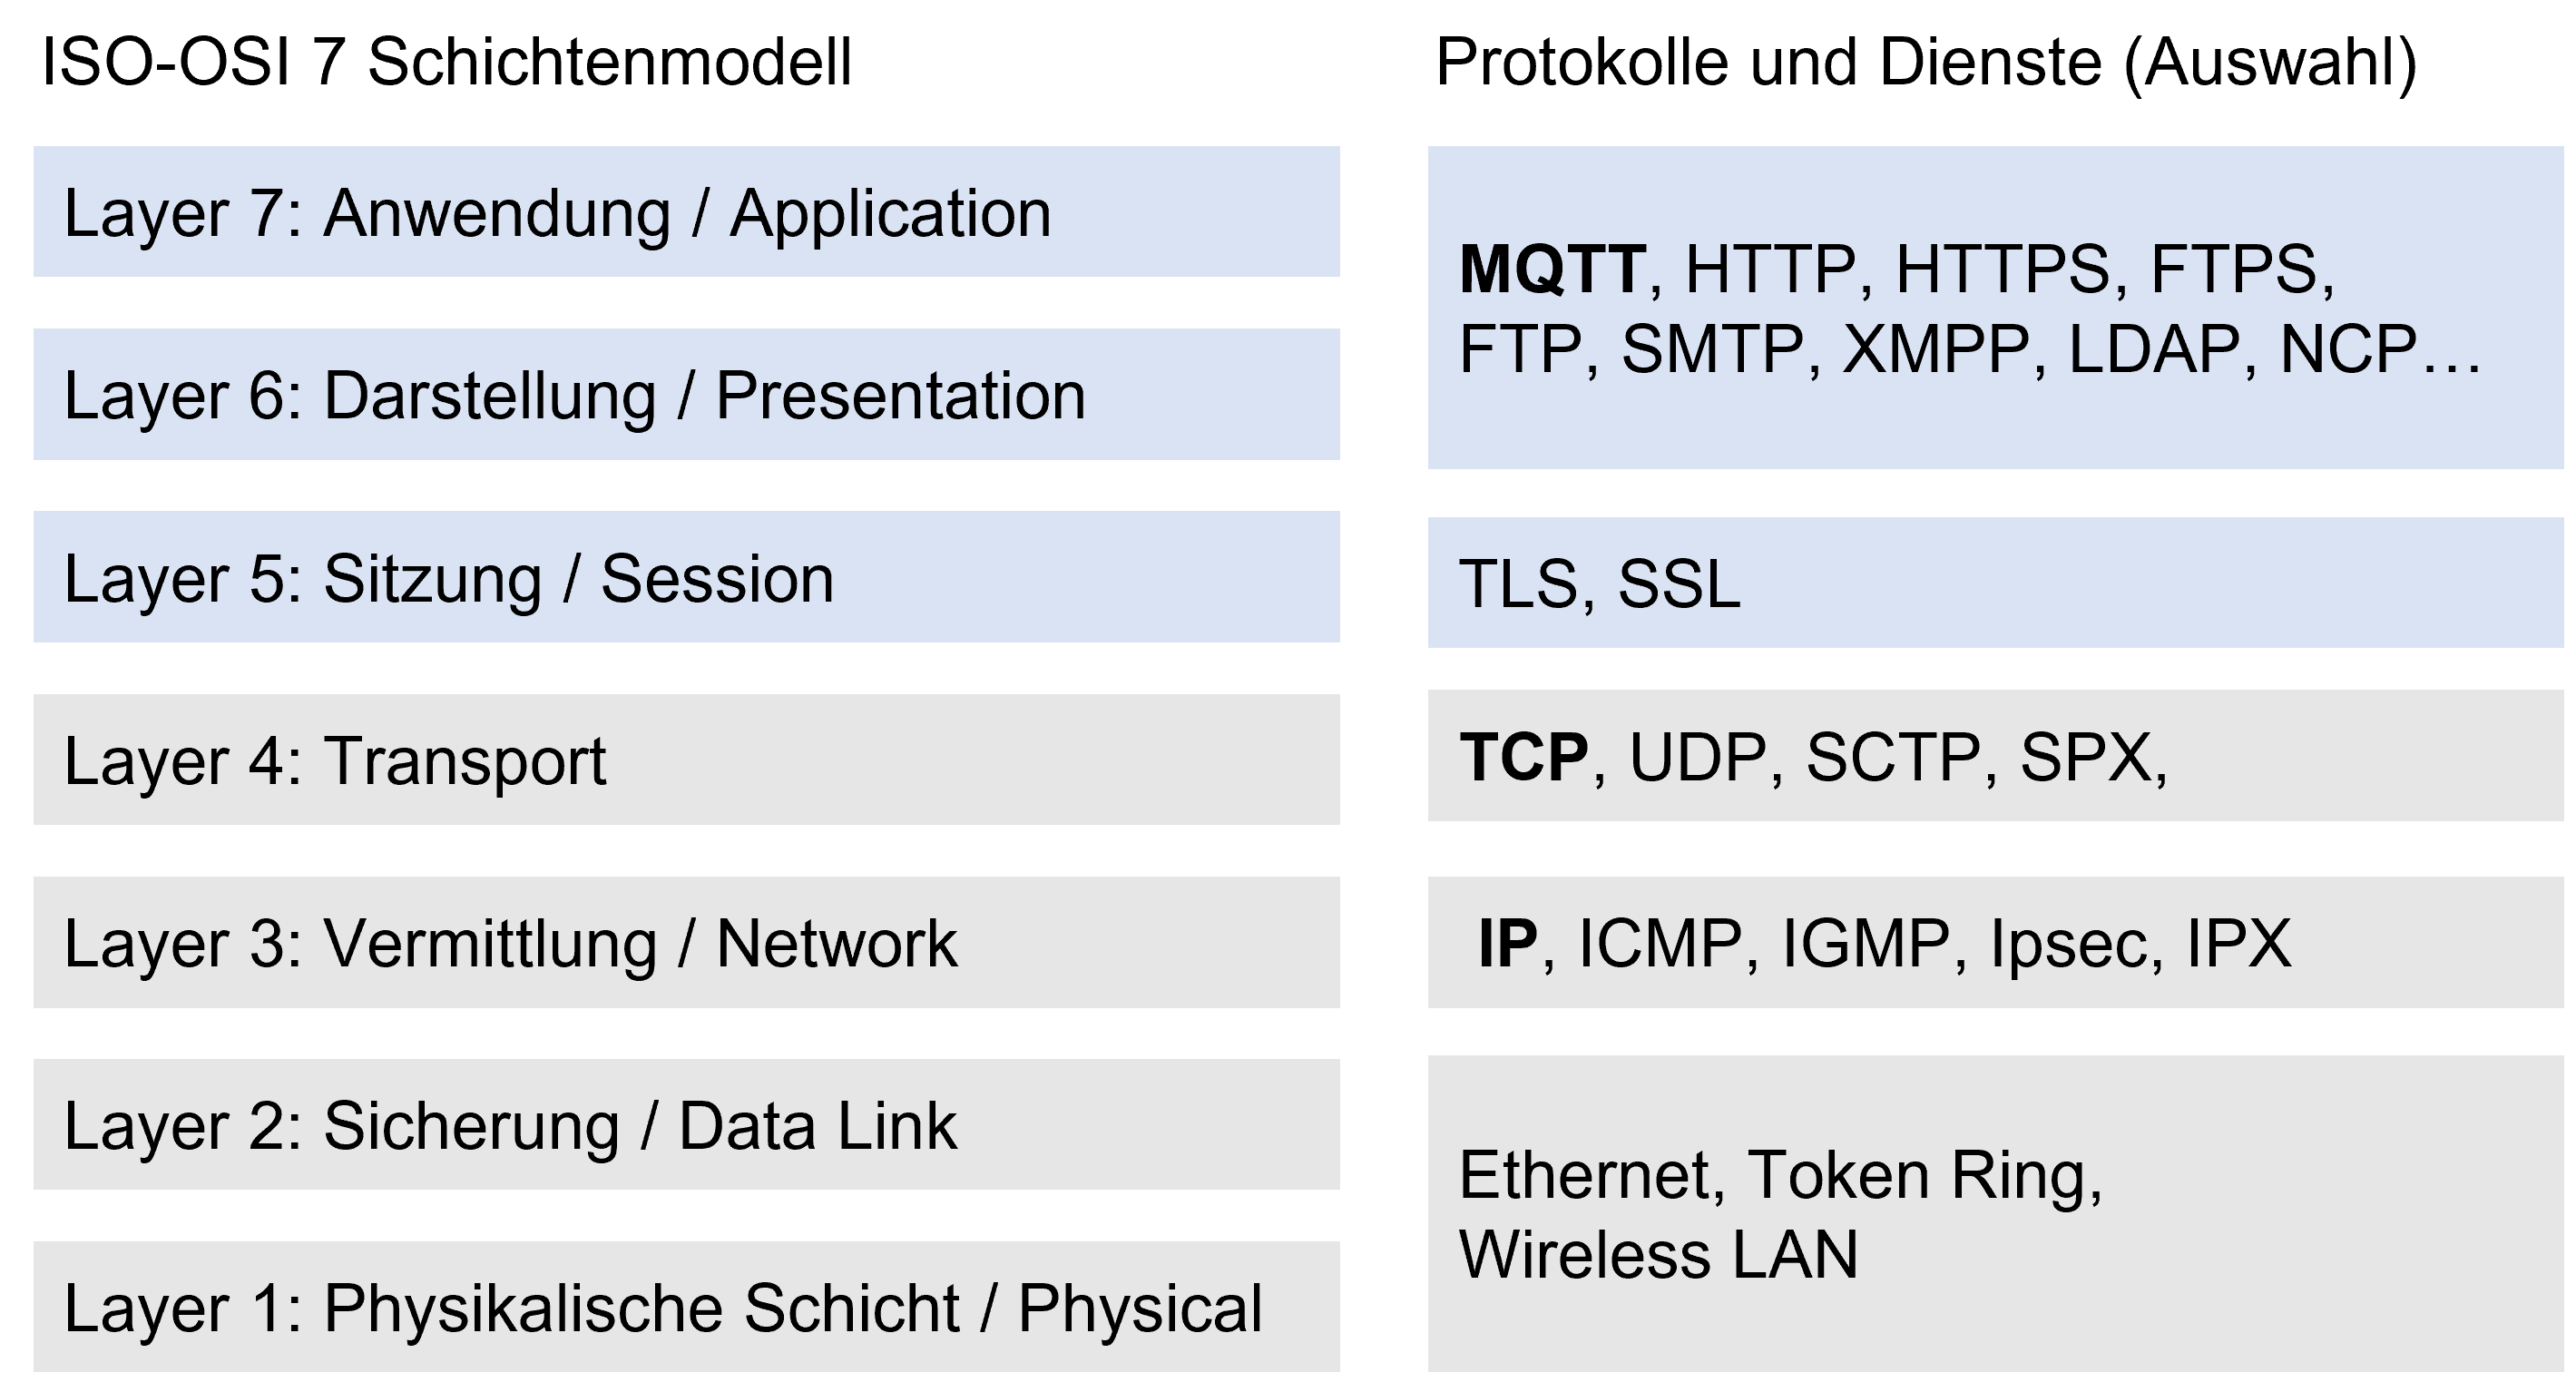
\includegraphics[width=0.6\textwidth,height=\textheight]{images/osi-modell.png}

}

\caption{\label{fig-osimodell}Das ISO OSI Schichtenmodell mit einer
Auswahl von Protokollen für die jeweilige Schicht. Das MQTT Protokoll
ist in der Schichten der Darstellungs- und Anwendungsschicht angesiedelt
und nutzt TCP/IP für die Datenübertragung über die IP Adressen der IoT
Geräte.}

\end{figure}%

\begin{description}
\tightlist
\item[ISO OSI Schichtenmodell\index{ISO/OSI Schichtenmodell}]
Das ISO OSI Schichtenmodell (Open Systems Interconnection Model) ist ein
konzeptuelles Referenzmodell welches die Funktionsweise von
Netzwerksystemen beschreibt mit dem Ziel Kommunikation über die
unterschiedlichen Technologien hinweg zu beschreiben von der Übertragung
von einzelnen Bits über den Datentransport bis hin zur Anwendung
beispielsweise HTTPS oder FTP (ISO 1994). Das ISO/OSI Schichtenmodell
besteht aus sieben hierarchisch aufgebauten Schichten und jeder
einzelnen Schicht ist eine Aufgabe zugeordnet, wobei das
Übertragungsmedium nicht definiert ist. Die Schichten eins bis vier sind
transportorientierte Schichten und die Schichten fünf bis sieben sind
anwendungsorientierte Schichten.
\item[Long Range Wide Area Network (LoRaWAN) oder LoRa\index{LoRaWAN}]
LoRaWan, Long Range Wide Area Network ermöglicht ein energieeffizientes
übertragen von kleinen Datenmengen über grosse Distanzen (bis 10km).
\end{description}

\section{Kommunikation}\label{kommunikation}

Zwei Kommunikationsparadigmen kommen in IoT Systemen zum Einsatz,
\emph{Publish-Subscribe} und \emph{Request-Response}. Je nach Szenario
und Anwendungsfall kommt der eine oder andere Ansatz zum Einsatz. In der
\emph{Publish-Subscribe} Kommunikation sind zwei Entitäten involviert,
der Publisher, der die Daten publiziert und der Subscriber, der die
Daten konsumiert, eine \emph{one-to-many Kommunication}. Dies ist gerade
in IoT Systemen von Vorteil, wo mehrere Geräte die Daten von einem Gerät
konsumieren können ohne, dass zu jedem einzelnen Gerät eine Verbindung
aufgebaut werden muss. Eine one-to-one Kommunikation ist hingehen eine
\emph{Request-Response} Kommunikation, in der Daten zwischen zwei
Entitäten ausgetauscht werden, wobei hier der Empfänger (Adresse) der
Nachricht oder der Daten bekannt sein muss. In der
\emph{Request-Response} Kommunikation ist der Server zentraler
Bestandteil der Kommunikation, wohingegen in der
\emph{Publish-Subscribe} Kommunikation der Broker zentraler Bestandteil
der Kommunikation ist (Hirmer 2023). Bei \emph{Publish-Subscribe} muss
der Broker bekannt sein wohingegen die Indentität der Publisher und
Subscriber nicht erforderlich ist.

\begin{figure}[H]

{\centering 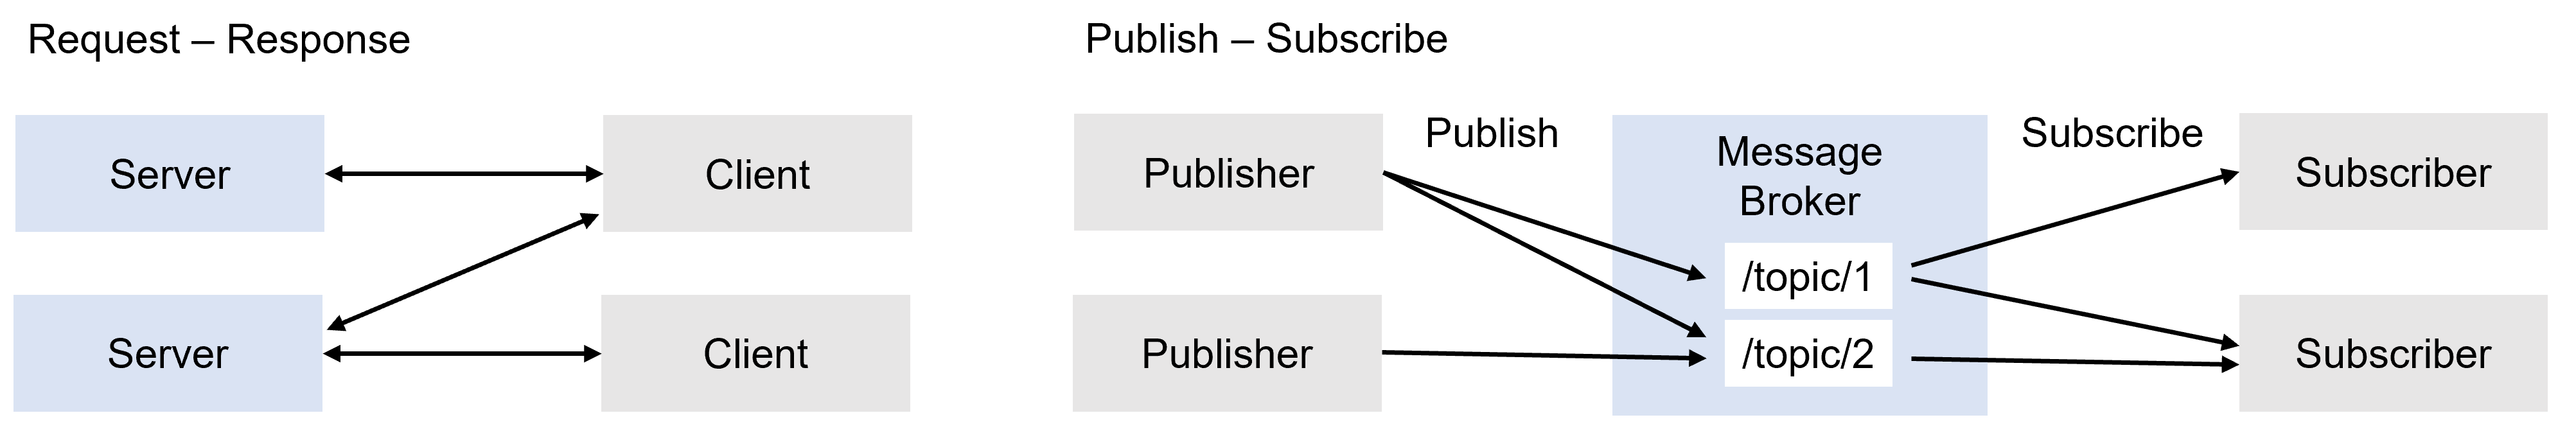
\includegraphics{images/publish-subcribe_request-response.png}

}

\caption{Kommunikationsparadigmen in der IoT Request-Response versus
Publish-Subscribe}

\end{figure}%

Die zentrale Komponente beim Publish-Subscribe Modells ist der Message
Broker, der für das Empfangen, Zwischenspeichern und die Vermittlung der
Nachrichten zu den Subscriber verantwortlich ist. Die Nachrichten oder
Datenpakete werden Topics (Themen) zugeordnert die hierarchisch
strukturiert sind. So können Subscriber gewisse Topics oder Untertopics
subscriben, wie beispielweise den Temperaturdaten einer Wetterstation
mit \emph{stationA/temperature}.

Message Broker können \emph{Quality of Service} parameter definieren,
die die Zuverlässigkeit der Nachrichtenübertragung definieren, ob
beispielsweise die Nachricht genau oder mindestens einmal zugestellt
werden soll. Dies geht jedoch zu Lasten der Performance, was gerade bei
Echtzeitkommunikation relevant ist. Einer der wesentlichen Vorteile des
Publish-Subscribe Modells ist, dass Publisher und Subscriber nicht
gleichzeitig online sein müssen, da der Broker die Nachrichten
zwischenspeichert und diese bei der nächsten Verbindung zustellt. Dies
ist ermöglicht eine asynchrone Kommunikation in Echtzeit, eine wichtige
Anforderung von IoT. Dies ist vorallem bei batteriebetriebenen Geräten
sinnvoll, die energiefizient arbeiten und folglich nicht kontinuierlich
online sind. Eines der verbreitesten Protokolle, die
\emph{Publish-Subscribe} umsetzen ist MQTT. In \textbf{GeoMQTT} kann
eine Nachricht mit einem Zeitstempel oder Interval und einer Geometrie
zusätzlich dem Topic name hinzugefügt werden. Dies ermöglicht dem
Subscriber zeitliche oder räumliche Filter zusätzlich zu den
thematischen \emph{Topic} Filter zu nutzen Herlé \emph{u.~a.} (2019).
Ein umfangreicherer offener Standard ist AMQP, seit 2010, der auch
\emph{request-response} Kommunikation ermöglicht\footnote{Diese
  Protokolle sind nach dem Entwurfsmuster (Design Pattern) Beobachter
  (Observer) implementiert}.

Eine weitere wichtige Anforderung an IoT ist die asynchrone
Kommunikation in Echtzeit. Synchrone Kommunikation in Echtzeit bedingt,
dass die Uhren synchron sind und beide zur gleichen Zeit kommunizieren,
was in vielen Anwendungsfällen der IoT nicht wünschenswert ist.

\section{MQTT - Message Queuing Telemetry Transport
Protocol}\label{mqtt---message-queuing-telemetry-transport-protocol}

Das MQTT Protokoll mit dem \emph{Publisher-Subscriber} Ansatz ermöglich
asynchrone Kommunikation von Events in Echtzeit in dem zwischen
Subscriber und Publisher ein \emph{Broker}-Server in der Kommunikation
dazwischen steht, der die Nachrichten zwischenspeichert. MQTT ist ein
Protokoll für die Kommunikation zwischen Geräten und Servern und wurde
ursprünglich für eine schlanke Datenübertragung über
Satellitenkommunikation entwickelt. MQTT ist ein offenes Protokoll, das
seit 1999 entwickelt wird, auf TCP/IP basiert und ab der Version 3.1
geöffnet wurde.

Der Publisher sendet \emph{publish} eine Nachricht zu einem Topic
(beispielsweise \emph{gebauede1/labor1/temperature}) mit einem
bestimmten \emph{Quality of Service} (at most once, at least once,
exactly once) Parameter. Der Broker speichert die Nachricht und sendet
diese an alle Subscriber, die dieses Topic abonnieren \emph{subscribe}.
\href{https://mosquitto.org}{Mosquitto} ist ein quelloffener Message
Broker, der die MQTT implementiert. Mosquitto ist schlank und eignet
sich für den Einsatz auf allen Geräten, von stromsparenden
Einplatinencomputern bis hin zu kompletten Servern. Eclipse Paho ist
eine quelloffene Implementierung von MQTT und bietet Bibliotheken in
verschiedenen Programmiersprachen wie Python, C++ oder Java an.

\section{Cloud, Edge und Fog}\label{cloud-edge-und-fog}

Mit zunehmender Rechenleistung auf IoT Geräten können diese vermehrt
selbst Daten prozessieren, was eine Verlagerung der Analyse ermöglicht.
Die Begriffe Cloud, Edge und Fog bezeichnen im wesentlichen wo in
Infrastrukturen die Datenprozessierung durchgeführt wird. In
\textbf{Cloud} Infrastrukturen erfolgt die Prozessierung zentralisiert
in der Cloud und grossen Recheninfrastrukturen, wohingegen
\textbf{Edge}-Computing eine Infrastruktur bezeichnet, in der die
lokalen Geräte selbst einen Teil der Daten dezentral und möglichst lokal
verarbeiten. Fog - ein von Cisco eingeführter Begriff - bezeichnet Cloud
Computing im lokalen Netzwerk, beispielsweise könnte ein
Transportunternehmen die Verwaltung der Datenprozessierung in der
eigenen Cloud durchführen.

\begin{figure}[H]

{\centering 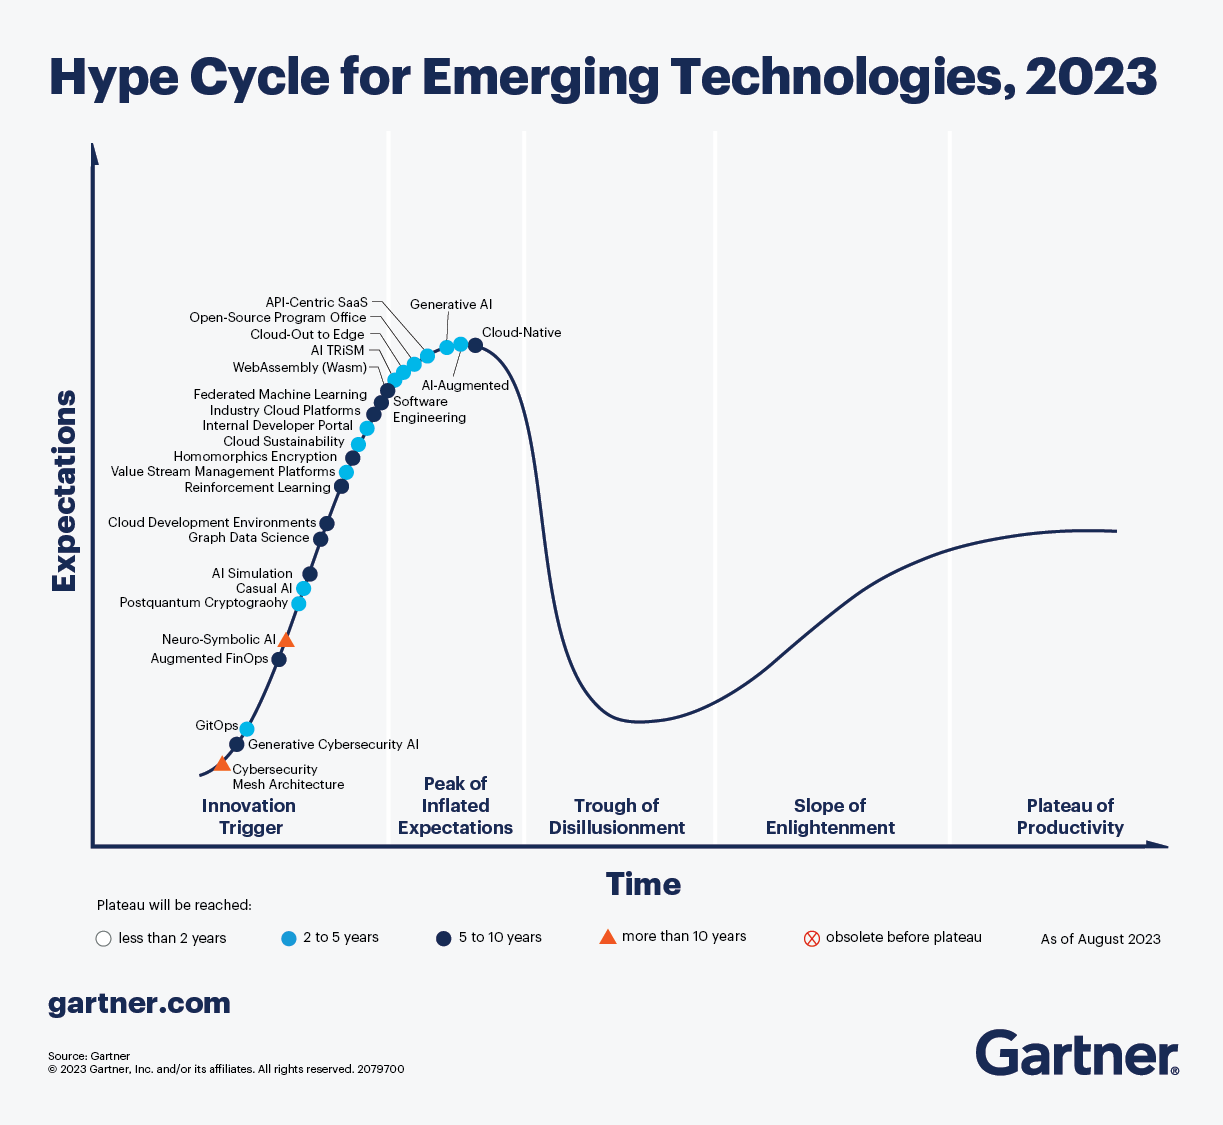
\includegraphics[width=0.5\textwidth,height=\textheight]{images/gartner_hypecycle_2023.png}

}

\caption{Im Gartner Hype Cycle for Emerging Technologies 2023 erreicht
der ``Hype'' \emph{Cloud-Out to Edge} den Peak of Inflated Expectations
(Gartner 2023)}

\end{figure}%

\chapter*{Literatur}\label{literatur}
\addcontentsline{toc}{chapter}{Literatur}

\markboth{Literatur}{Literatur}

\phantomsection\label{refs}
\begin{CSLReferences}{1}{0}
\bibitem[\citeproctext]{ref-ams2022}
AMS OSRAM Group, 2022.
\href{https://ams.com/documents/20143/36005/AS7262/_DS000486/_5-00.pdf}{Datasheet
{AS7262} 6-{Channel Visible Spectral}\_{ID Device} with {Electronic
Shutter} and {Smart Interface}}.

\bibitem[\citeproctext]{ref-ariza2022}
Ariza, J.Á. und Baez, H., 2022.
\href{https://doi.org/10.1002/cae.22439}{Understanding the Role of
Single-Board Computers in Engineering and Computer Science Education:
{A} Systematic Literature Review}. \emph{Computer Applications in
Engineering Education}, 30 (1), 304--329.

\bibitem[\citeproctext]{ref-ashton2009}
Ashton, K., 2009. That {„Internet of Things``} Thing. \emph{RFID
journal}, 22 (7), 97--114.

\bibitem[\citeproctext]{ref-celebi2020}
Celebi, H.B., Pitarokoilis, A., und Skoglund, M., 2020.
\href{https://doi.org/10.1007/978-3-030-42500-5_2}{Wireless
{Communication} for the {Industrial IoT}}. \emph{In}: I. Butun, Hrsg.
\emph{Industrial {IoT} : {Challenges}, {Design Principles},
{Applications}, and {Security}}. {Cham}: {Springer International
Publishing}, 57--94.

\bibitem[\citeproctext]{ref-gartner2023}
Gartner, 2023.
\href{https://www.gartner.com/en/articles/what-s-new-in-the-2023-gartner-hype-cycle-for-emerging-technologies}{4
{Exciting New Trends} in the {Gartner Emerging Technologies Hype
Cycle}}. \emph{Gartner}.

\bibitem[\citeproctext]{ref-bosch2022}
\href{https://www.bosch-sensortec.com/products/environmental-sensors/gas-sensors/bme688/}{Gas
Sensor {BME688}}, o.~J. \emph{Bosch Sensortec}.

\bibitem[\citeproctext]{ref-gore1998}
Gore, A., 1998.
\href{https://doi.org/10.1080/00050348.1998.10558728}{The {Digital
Earth}}. \emph{Australian Surveyor}, 43 (2), 89--91.

\bibitem[\citeproctext]{ref-granell2020}
Granell, C., Kamilaris, A., Kotsev, A., Ostermann, F.O., und Trilles,
S., 2020. \href{https://doi.org/10.1007/978-981-32-9915-3_11}{Internet
of {Things}}. \emph{In}: H. Guo, M.F. Goodchild, und A. Annoni, Hrsg.
\emph{Manual of {Digital Earth}}. {Singapore}: {Springer}, 387--423.

\bibitem[\citeproctext]{ref-grimm2023}
Grimm, D., 2023.
\href{https://moodle.fhnw.ch/course/view.php?id=37277}{2030
{Geod{ä}tische Messtechnik GMT I}}.

\bibitem[\citeproctext]{ref-herle2019}
Herlé, S., Bill, R., und Blankenbach, J.M., 2019.
\href{https://publications.rwth-aachen.de/record/772603/}{{A
GeoEvent-driven architecture based on GeoMQTT for the Geospatial IoT}}.
phdthesis No. RWTH-2019-10695. Dissertation, Rheinisch-Westf{ä}lische
Technische Hochschule Aachen, 2019.

\bibitem[\citeproctext]{ref-hirmer2023}
Hirmer, P., 2023.
\href{https://doi.org/10.1007/978-3-031-18884-8_2}{Foundations}.
\emph{In}: P. Hirmer, Hrsg. \emph{Model-{Based Approaches} to the
{Internet} of {Things}}. {Cham}: {Springer International Publishing},
7--15.

\bibitem[\citeproctext]{ref-influxdata2023}
influxdata, 2023.
\href{https://docs.influxdata.com/influxdb/v2/get-started/}{Get Started
with {InfluxDB} {\textbar} {InfluxDB OSS} v2 {Documentation}}.

\bibitem[\citeproctext]{ref-tdk2021}
InvenSense, T., 2021.
\href{https://invensense.tdk.com/wp-content/uploads/2021/10/DS-000189-ICM-20948-v1.5.pdf}{{ICM-20948
World}'s {Lowest Power} 9-{Axis MEMS MotionTracking}™ {Device}}.

\bibitem[\citeproctext]{ref-iso1994}
ISO, 1994. \href{https://www.iso.org/standard/20269.html}{{ISO}/{IEC}
7498-1:1994}. \emph{ISO}.

\bibitem[\citeproctext]{ref-ITU2005}
ITU, 2005.
\emph{\href{https://www.itu.int:443/en/publications/gs/Pages/publications.aspx?parent=S-POL-IR.IT-2005/&media=paper}{{ITU
Internet Reports} 2005: {The Internet} of {Things}}}. {Geneva}:
{International Telecommunication Union}.

\bibitem[\citeproctext]{ref-jensen2020}
Jensen, K., 2020. \emph{White {Paper Chip-scale} Spectral Sensing:
Understanding the New Uses for Ultra-Precise Light-Source Measurement}.
{Premstaetten, Austria}: {AMS}, White \{\{Paper\}\}.

\bibitem[\citeproctext]{ref-kamilaris2018}
Kamilaris, A. und Ostermann, F.O., 2018.
\href{https://doi.org/10.3390/ijgi7070269}{Geospatial {Analysis} and the
{Internet} of {Things}}. \emph{ISPRS International Journal of
Geo-Information}, 7 (7), 269.

\bibitem[\citeproctext]{ref-laska2018}
Laska, M., Herle, S., Klamma, R., und Blankenbach, J., 2018.
\href{https://doi.org/10.3390/ijgi7070238}{A {Scalable Architecture} for
{Real-Time Stream Processing} of {Spatiotemporal IoT Stream
Data}---{Performance Analysis} on the {Example} of {Map Matching}}.
\emph{ISPRS International Journal of Geo-Information}, 7 (7), 238.

\bibitem[\citeproctext]{ref-leicageosystems2022}
Leica Geosystems, 2022. Leica {TS60}/{MS60}/{TM60 Gebrauchsanweisung}.

\bibitem[\citeproctext]{ref-links2019}
Links, C., 2019.
\href{https://www.qorvo.com/design-hub/blog/iot-standards-the-end-game}{{IoT
Standards}: {The End Game} - {Qorvo}}.

\bibitem[\citeproctext]{ref-maximintegrated2020}
maxim integrated, 2020. {MAX30101 High-Sensitivity Pulse Oximeter} and
{Heart-Rate Sensor} for {Wearable Health}.

\bibitem[\citeproctext]{ref-melexis2019}
Melexis, 2019.
\href{https://media.melexis.com/-/media/files/documents/datasheets/mlx90640-datasheet-melexis.pdf}{{MLX90640}
32x24 {IR} Array {Datasheet}}.

\bibitem[\citeproctext]{ref-rogers2006}
Rogers, Y., 2006. \href{https://doi.org/10.1007/11853565_24}{Moving on
from {Weiser}'s {Vision} of {Calm Computing}: {Engaging UbiComp
Experiences}}. \emph{In}: P. Dourish und A. Friday, Hrsg.
\emph{{UbiComp} 2006: {Ubiquitous Computing}}. {Berlin, Heidelberg}:
{Springer}, 404--421.

\bibitem[\citeproctext]{ref-salvador2003}
Salvador, T. und Anderson, K., 2003.
\href{https://doi.org/10.1007/978-3-540-39653-6_19}{Practical
{Considerations} of {Context} for {Context Based Systems}: {An Example}
from an {Ethnographic Case Study} of a {Man Diagnosed} with {Early Onset
Alzheimer}'s {Disease}}. \emph{In}: A.K. Dey, A. Schmidt, und J.F.
McCarthy, Hrsg. \emph{{UbiComp} 2003: {Ubiquitous Computing}}. {Berlin,
Heidelberg}: {Springer}, 243--255.

\bibitem[\citeproctext]{ref-sliney2016}
Sliney, D.H., 2016. \href{https://doi.org/10.1038/eye.2015.252}{What Is
Light? {The} Visible Spectrum and Beyond}. \emph{Eye}, 30 (2), 222--229.

\bibitem[\citeproctext]{ref-st2021}
STMicroelectronics, 2021.
\href{https://www.st.com/resource/en/datasheet/vl53l5cx.pdf}{{VL53L5CX}
- {Datasheet} - {Time-of-Flight} 8x8 Multizone Ranging Sensor with Wide
Field of View}.

\bibitem[\citeproctext]{ref-st2023}
STMicroelectronics, 2023.
\href{https://www.st.com/resource/en/application/_note/an5894-description-of-the-fields-of-view-of-stmicroelectronics-timeofflight-sensors-stmicroelectronics.pdf}{Description
of the Fields of View of {STMicroelectronics}' {Time-of-Flight}
Sensors}.

\bibitem[\citeproctext]{ref-trilles2017}
Trilles, S., Belmonte, Ò., Schade, S., und Huerta, J., 2017.
\href{https://doi.org/10.1080/17538947.2016.1209583}{A
Domain-Independent Methodology to Analyze {IoT} Data Streams in
Real-Time. {A} Proof of Concept Implementation for Anomaly Detection
from Environmental Data}. \emph{International Journal of Digital Earth},
10 (1), 103--120.

\bibitem[\citeproctext]{ref-upton2022}
Upton, E., 2022.
\href{https://www.raspberrypi.com/news/supply-chain-update-its-good-news/}{Supply
Chain Update - It's Good News!} \emph{Raspberry Pi}.

\bibitem[\citeproctext]{ref-wiegerling2013}
Wiegerling, K., 2013.
\href{https://doi.org/10.1007/978-3-476-05333-6_71}{{Ubiquitous
Computing}}. \emph{In}: A. Grunwald und M. Simonidis-Puschmann, Hrsg.
\emph{{Handbuch Technikethik}}. {Stuttgart}: {J.B. Metzler}, 374--378.

\bibitem[\citeproctext]{ref-zaheeruddin2020}
Zaheeruddin und Gupta, H., 2020.
\href{https://doi.org/10.1007/978-3-030-37468-6_1}{Foundation of {IoT}:
{An Overview}}. \emph{In}: M. Alam, K.A. Shakil, und S. Khan, Hrsg.
\emph{Internet of {Things} ({IoT}): {Concepts} and {Applications}}.
{Cham}: {Springer International Publishing}, 3--24.

\end{CSLReferences}

\part{Praktika}

\chapter*{E01 Luftqualitätmessung}\label{e01-luftqualituxe4tmessung}
\addcontentsline{toc}{chapter}{E01 Luftqualitätmessung}

\markboth{E01 Luftqualitätmessung}{E01 Luftqualitätmessung}

Ziel dieser ersten Übung ist es den BME688 Sensor kennen zu lernen und
die Sensordaten auszulesen. Der BME688 ist ein 4-in-1 Sensor für
Temperatur, Luftdruck, Luftfeuchtigkeit und Gas Scanner VOC. Der Sensor
verfügt über eine I2C Schnittstelle, die mit der Python Library
\href{https://github.com/pimoroni/bme680-python}{bme680-python}
angesteuert und die Sensordaten ausgelesen werden können.

\textbf{Vorbereitung}

\begin{itemize}
\tightlist
\item
  Lest das Kapitel im Anhang zu \href{A1_Rasperry_Pi.qmd}{Raspberry Pi}

  \begin{itemize}
  \tightlist
  \item
    Konzentriere Dich auf die wichtigsten Details zur Inbetriebnahme des
    Raspberry Pi
  \end{itemize}
\item
  Lest die Dokumentation zum BME688 Sensor Gas Sensor {BME688} (o.~J.)

  \begin{itemize}
  \tightlist
  \item
    Konzentriere Dich auf die Beschreibung der Schnittstelle und
    technische Spezifikation auf dem Datenblatt
  \end{itemize}
\end{itemize}

\begin{figure}[H]

{\centering 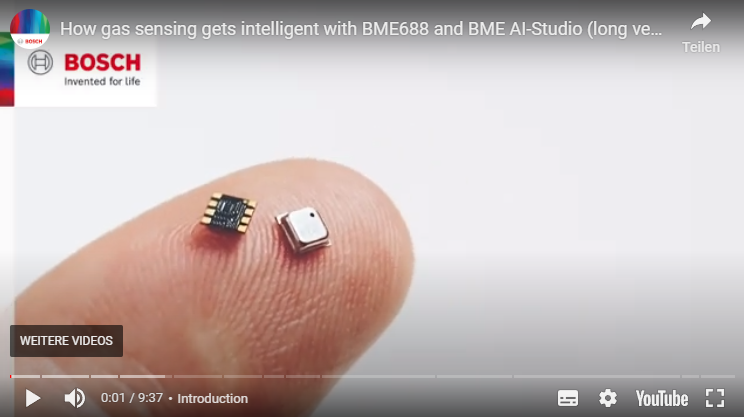
\includegraphics{images/youtube_bosch_bme688.png}

}

\caption{Youtube Video: How gas sensing gets intelligent with BME688 and
BME AI-Studio}

\end{figure}%

\begin{longtable}[]{@{}
  >{\raggedright\arraybackslash}p{(\columnwidth - 2\tabcolsep) * \real{0.2083}}
  >{\raggedright\arraybackslash}p{(\columnwidth - 2\tabcolsep) * \real{0.7917}}@{}}
\toprule\noalign{}
\begin{minipage}[b]{\linewidth}\raggedright
\textbf{Unterlagen}
\end{minipage} & \begin{minipage}[b]{\linewidth}\raggedright
\end{minipage} \\
\midrule\noalign{}
\endhead
\bottomrule\noalign{}
\endlastfoot
Produkt &
\href{https://shop.pimoroni.com/products/bme688-breakout}{BME688 4-in-1
Air Quality Breakout} \\
Datenblatt &
\href{https://www.bosch-sensortec.com/media/boschsensortec/downloads/datasheets/bst-bme688-ds000.pdf}{Bosch
Datasheet BME 688} \\
GitHub & \href{https://github.com/pimoroni/bme680-python}{bme680-python
Library mit Beispielen} \\
Tutorial &
\href{https://learn.pimoroni.com/article/getting-started-with-bme680-breakout}{Getting
started with BME680 Breakout} \\
\end{longtable}

\section*{\texorpdfstring{BME688\index{BME688}}{BME688}}\label{bme688}
\addcontentsline{toc}{section}{BME688\index{BME688}}

\markright{BME688\index{BME688}}

BME688 - Bosch Sensor für Temperatur, Luftdruck, Luftfeuchtigkeit, Gas
Scanner VOC (Abbildung~\ref{fig-bme688})

\begin{itemize}
\tightlist
\item
  Temperatur +/-0.5°C (-40° .. -85°)
\item
  Luftdruck +/-0.12hPa (300\ldots1100hPa)
\item
  Luftfeuchtigkeit +/-3\% (0 \ldots100\%)
\item
  Gas Scanner VOC, VSCs (AI)
\item
  Python, C Library
\item
  Raspberry Pi Pins 1,3,5,7,9
\end{itemize}

\begin{figure}

\centering{

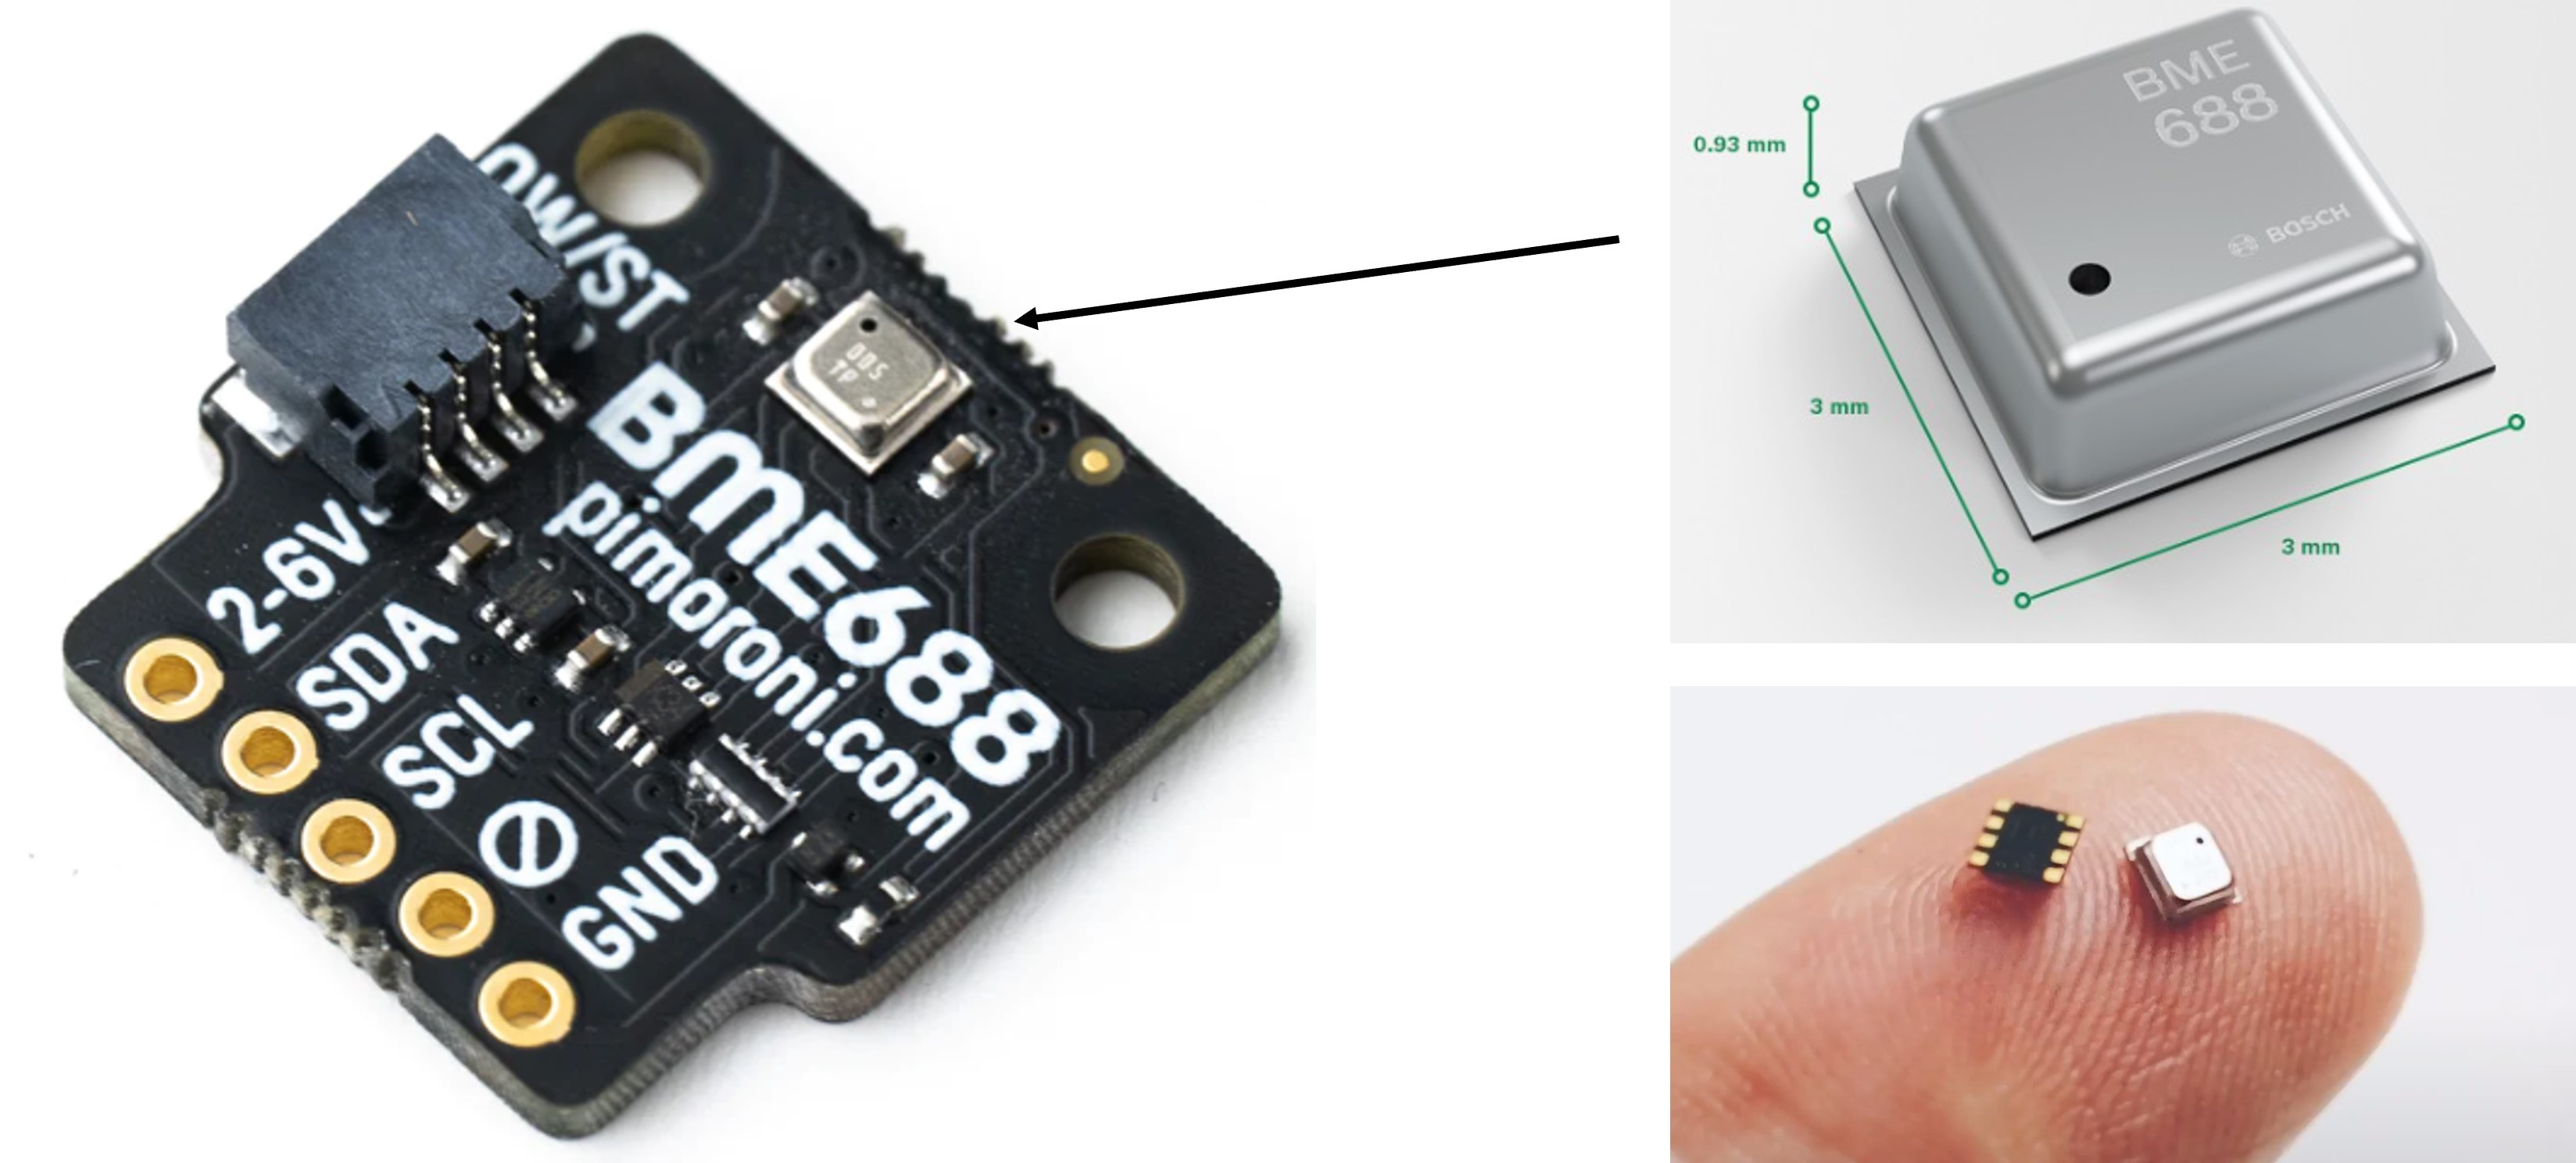
\includegraphics{images/BME688_wide.jpg}

}

\caption{\label{fig-bme688}BME688 Bosch Sensor für Luftqualitätsmessung
mit Referenzbild für den Grössenvergleich}

\end{figure}%

\section*{Übungsaufbau}\label{uxfcbungsaufbau}
\addcontentsline{toc}{section}{Übungsaufbau}

\markright{Übungsaufbau}

\begin{itemize}
\tightlist
\item
  Schliesse den Raspberry Pi an Monitor, Keyboard und Maus an oder
  verbinde Dich mit diesem über SSH (und SFTP).
\item
  Erstelle auf dem Raspberry Pi im \texttt{Documents} Ordner einen neuen
  Ordner \texttt{BME688}, in welchem Du Änderungen und neue Dateien für
  diese Übung speichern kannst.
\item
  Schliesse den Sensor \textbf{BME688} an den Raspberry Pi über die
  Breakout Garden \textbf{I2C} Schnittstelle an.
\end{itemize}

\begin{boxtitle}{Hinweis}{colPrimary}

\textbf{Sensor Ausrichtung beachten}

Beim Anschliessen der Sensoren in die Schnittstellen des Breakout Garden
\textbf{unbedingt} die korrekte Ausrichtung beachten! Die Beschriftung
der Anschlüsse auf dem Sensor und dem Breakout Garden müssen
übereinstimmen!

\begin{figure}[H]

{\centering \includegraphics{images/raspberry_pi_correct_sensor_mount.png}

}

\caption{Sensor links korrekt angeschlossen, rechts falsch ausgerichtet
angeschlossen.}

\end{figure}%

\end{boxtitle}

\subsection*{Kontrolle der Hardware}\label{kontrolle-der-hardware}
\addcontentsline{toc}{subsection}{Kontrolle der Hardware}

Kontrolliere mit dem Befehl \texttt{i2cdetect\ -y\ 1} ob der Raspberry
Pi mit dem Sensor verbunden ist und der Raspberry Pi Zugriff auf den
Sensor hat. Erscheint eine Zahl, dann hat der Raspberry Pi den Sensor
auf dem I2C Bus erkannt. Falls Du mehr über das Program und den Befehl
wissen möchtest, kannst Du mit dem Befehl \texttt{man\ i2cdetect} das
Manual \texttt{man} aufrufen.

\begin{Shaded}
\begin{Highlighting}[]
\ExtensionTok{i2cdetect} \AttributeTok{{-}y}\NormalTok{ 1}
     \ExtensionTok{0}\NormalTok{  1  2  3  4  5  6  7  8  9  a  b  c  d  e  f}
\ExtensionTok{00:}                         \AttributeTok{{-}{-}} \AttributeTok{{-}{-}} \AttributeTok{{-}{-}} \AttributeTok{{-}{-}} \AttributeTok{{-}{-}} \AttributeTok{{-}{-}} \AttributeTok{{-}{-}} \AttributeTok{{-}{-}} 
\ExtensionTok{10:} \AttributeTok{{-}{-}} \AttributeTok{{-}{-}} \AttributeTok{{-}{-}} \AttributeTok{{-}{-}} \AttributeTok{{-}{-}} \AttributeTok{{-}{-}} \AttributeTok{{-}{-}} \AttributeTok{{-}{-}} \AttributeTok{{-}{-}} \AttributeTok{{-}{-}} \AttributeTok{{-}{-}} \AttributeTok{{-}{-}} \AttributeTok{{-}{-}} \AttributeTok{{-}{-}} \AttributeTok{{-}{-}} \AttributeTok{{-}{-}} 
\ExtensionTok{20:} \AttributeTok{{-}{-}} \AttributeTok{{-}{-}} \AttributeTok{{-}{-}} \AttributeTok{{-}{-}} \AttributeTok{{-}{-}} \AttributeTok{{-}{-}} \AttributeTok{{-}{-}} \AttributeTok{{-}{-}} \AttributeTok{{-}{-}} \AttributeTok{{-}{-}} \AttributeTok{{-}{-}} \AttributeTok{{-}{-}} \AttributeTok{{-}{-}} \AttributeTok{{-}{-}} \AttributeTok{{-}{-}} \AttributeTok{{-}{-}} 
\ExtensionTok{30:} \AttributeTok{{-}{-}} \AttributeTok{{-}{-}} \AttributeTok{{-}{-}} \AttributeTok{{-}{-}} \AttributeTok{{-}{-}} \AttributeTok{{-}{-}} \AttributeTok{{-}{-}} \AttributeTok{{-}{-}} \AttributeTok{{-}{-}} \AttributeTok{{-}{-}} \AttributeTok{{-}{-}} \AttributeTok{{-}{-}} \AttributeTok{{-}{-}} \AttributeTok{{-}{-}} \AttributeTok{{-}{-}} \AttributeTok{{-}{-}} 
\ExtensionTok{40:} \AttributeTok{{-}{-}} \AttributeTok{{-}{-}} \AttributeTok{{-}{-}} \AttributeTok{{-}{-}} \AttributeTok{{-}{-}} \AttributeTok{{-}{-}} \AttributeTok{{-}{-}} \AttributeTok{{-}{-}} \AttributeTok{{-}{-}} \AttributeTok{{-}{-}} \AttributeTok{{-}{-}} \AttributeTok{{-}{-}} \AttributeTok{{-}{-}} \AttributeTok{{-}{-}} \AttributeTok{{-}{-}} \AttributeTok{{-}{-}} 
\ExtensionTok{50:} \AttributeTok{{-}{-}} \AttributeTok{{-}{-}} \AttributeTok{{-}{-}} \AttributeTok{{-}{-}} \AttributeTok{{-}{-}} \AttributeTok{{-}{-}} \AttributeTok{{-}{-}} \AttributeTok{{-}{-}} \AttributeTok{{-}{-}} \AttributeTok{{-}{-}} \AttributeTok{{-}{-}} \AttributeTok{{-}{-}} \AttributeTok{{-}{-}} \AttributeTok{{-}{-}} \AttributeTok{{-}{-}} \AttributeTok{{-}{-}} 
\ExtensionTok{60:} \AttributeTok{{-}{-}} \AttributeTok{{-}{-}} \AttributeTok{{-}{-}} \AttributeTok{{-}{-}} \AttributeTok{{-}{-}} \AttributeTok{{-}{-}} \AttributeTok{{-}{-}} \AttributeTok{{-}{-}} \AttributeTok{{-}{-}} \AttributeTok{{-}{-}} \AttributeTok{{-}{-}} \AttributeTok{{-}{-}} \AttributeTok{{-}{-}} \AttributeTok{{-}{-}} \AttributeTok{{-}{-}} \AttributeTok{{-}{-}} 
\ExtensionTok{70:} \AttributeTok{{-}{-}} \AttributeTok{{-}{-}} \AttributeTok{{-}{-}} \AttributeTok{{-}{-}} \AttributeTok{{-}{-}} \AttributeTok{{-}{-}}\NormalTok{ 76 }\AttributeTok{{-}{-}}  
\end{Highlighting}
\end{Shaded}

\texttt{i2cdetect} installieren, falls das Programm nicht existiert:

\begin{Shaded}
\begin{Highlighting}[]
\FunctionTok{sudo}\NormalTok{ apt{-}get update }
\FunctionTok{sudo}\NormalTok{ apt install python3{-}smbus}
\FunctionTok{sudo}\NormalTok{ apt install i2c{-}tools}
\end{Highlighting}
\end{Shaded}

\textbf{Hinweis:} Damit der Befehl \texttt{i2cdetect} funktioniert, muss
der I2C Bus aktiviert sein. Dies kann mit dem Befehl
\texttt{sudo\ raspi-config} im Menü \texttt{Interfacing\ Options} und
\texttt{I2C} aktiviert werden.

\subsection*{Kontrolle der
Installation}\label{kontrolle-der-installation}
\addcontentsline{toc}{subsection}{Kontrolle der Installation}

Teste ob die für die Übung erforderlichen Python Libraries installiert
sind.

\phantomsection\label{annotated-cell-4}%
\begin{Shaded}
\begin{Highlighting}[]
\ExtensionTok{python} \AttributeTok{{-}c} \StringTok{"import math"}
\ExtensionTok{0} \hspace*{\fill}\NormalTok{\circled{1}}
\ExtensionTok{python} \AttributeTok{{-}c} \StringTok{"import numpy"}
\ExtensionTok{Traceback} \ErrorTok{(}\ExtensionTok{most}\NormalTok{ recent call last}\KeywordTok{)}\BuiltInTok{:} \hspace*{\fill}\NormalTok{\circled{2}}
  \ExtensionTok{File} \StringTok{"\textless{}string\textgreater{}"}\NormalTok{, line 1, in }\OperatorTok{\textless{}}\NormalTok{module}\OperatorTok{\textgreater{}} 
\ExtensionTok{ImportError:}\NormalTok{ No module named numpy }
\end{Highlighting}
\end{Shaded}

\begin{description}
\tightlist
\item[\circled{1}]
\texttt{math} Modul existiert
\item[\circled{2}]
\texttt{numpy} Modul existiert nicht
\end{description}

Installiere das Modul mit folgendem Befehl, falls es nicht installiert
ist.

\begin{Shaded}
\begin{Highlighting}[]
\FunctionTok{sudo}\NormalTok{ pip3 install bme680}
\end{Highlighting}
\end{Shaded}

\subsection*{Kopiere (Clone) die Library mit den Beispielen auf den
Raspberry
Pi}\label{kopiere-clone-die-library-mit-den-beispielen-auf-den-raspberry-pi}
\addcontentsline{toc}{subsection}{Kopiere (Clone) die Library mit den
Beispielen auf den Raspberry Pi}

Wechsle in den Ordner \emph{Documents} und kopiere mit folgenden
Befehlen die Library auf Deinen Raspberry Pi.

\begin{Shaded}
\begin{Highlighting}[]
\BuiltInTok{cd}\NormalTok{ Documents}
\FunctionTok{git}\NormalTok{ clone https://github.com/pimoroni/bme680{-}python }
\BuiltInTok{cd}\NormalTok{ bme680{-}python/examples}
\end{Highlighting}
\end{Shaded}

\section*{Aufgabe 1: Sensormessungen
ausführen}\label{aufgabe-1-sensormessungen-ausfuxfchren}
\addcontentsline{toc}{section}{Aufgabe 1: Sensormessungen ausführen}

\markright{Aufgabe 1: Sensormessungen ausführen}

Teste das Beispiel \texttt{read-all.py} im Ordner \emph{examples}.
Dieses Beispiel gibt die Temperatur, Luftdruck und Luftfeuchtigkeit des
Sensors BME 688 aus.

\begin{Shaded}
\begin{Highlighting}[]
\ExtensionTok{python3}\NormalTok{ read{-}all.py}
\end{Highlighting}
\end{Shaded}

Mit \texttt{Ctrl+c} kann das Script wieder gestopppt werden. Die Ausgabe
sollte in etwa so aussehen (gekürzt):

\begin{Shaded}
\begin{Highlighting}[]
\CommentTok{\# Output Beispiel}
\ExtensionTok{read{-}all.py} \AttributeTok{{-}}\NormalTok{ Displays temperature, pressure, humidity, and gas.}
\ExtensionTok{Press}\NormalTok{ Ctrl+C to exit!}

\ExtensionTok{Calibration}\NormalTok{ data:}
\ExtensionTok{par\_gh1:} \AttributeTok{{-}10}
\ExtensionTok{…}

\ExtensionTok{Initial}\NormalTok{ reading:}
\ExtensionTok{gas\_index:}\NormalTok{ 0}
\ExtensionTok{gas\_resistance:}\NormalTok{ 1338124.79581836}
\ExtensionTok{heat\_stable:}\NormalTok{ False}
\ExtensionTok{humidity:}\NormalTok{ 44.397}
\ExtensionTok{meas\_index:}\NormalTok{ 0}
\ExtensionTok{pressure:}\NormalTok{ 990.82}
\ExtensionTok{status:}\NormalTok{ 32}
\ExtensionTok{temperature:}\NormalTok{ 28.89}

\ExtensionTok{Polling:}
\ExtensionTok{28.89}\NormalTok{ C,990.82 hPa,44.39 \%RH}
\ExtensionTok{28.91}\NormalTok{ C,990.82 hPa,44.37 \%RH,5684.846331497602 Ohms}
\ExtensionTok{28.94}\NormalTok{ C,990.80 hPa,44.31 \%RH,5684.846331497602 Ohms}
\ExtensionTok{28.97}\NormalTok{ C,990.81 hPa,44.24 \%RH,5684.846331497602 Ohms}
\ExtensionTok{29.00}\NormalTok{ C,990.81 hPa,44.19 \%RH,5684.846331497602 Ohms}
\ExtensionTok{29.03}\NormalTok{ C,990.82 hPa,44.12 \%RH,5684.846331497602 Ohms}
\end{Highlighting}
\end{Shaded}

Folgendes Code Snippet zeigt eine gekürtzte Version des read-all.py
Python Beispiels, der die \emph{Temperatur}, \emph{Luftdruck} und
\emph{Luftfeuchtigkeit} mit der BME680 Library ausgibt.

\phantomsection\label{annotated-cell-9}%
\begin{Shaded}
\begin{Highlighting}[]
\CommentTok{\#!/usr/bin/env python}
\ImportTok{import}\NormalTok{ bme680}
\ControlFlowTok{try}\NormalTok{:                                               }
\NormalTok{    sensor }\OperatorTok{=}\NormalTok{ bme680.BME680(bme680.I2C\_ADDR\_PRIMARY) }\hspace*{\fill}\NormalTok{\circled{1}}
\ControlFlowTok{except}\NormalTok{ (}\PreprocessorTok{RuntimeError}\NormalTok{, }\PreprocessorTok{IOError}\NormalTok{):}
\NormalTok{    sensor }\OperatorTok{=}\NormalTok{ bme680.BME680(bme680.I2C\_ADDR\_SECONDARY) }

\CommentTok{\# Oversampling Einstellungen}
\NormalTok{sensor.set\_humidity\_oversample(bme680.OS\_2X) }\hspace*{\fill}\NormalTok{\circled{2}}
\NormalTok{sensor.set\_pressure\_oversample(bme680.OS\_4X) }
\NormalTok{sensor.set\_temperature\_oversample(bme680.OS\_8X) }
\NormalTok{sensor.set\_filter(bme680.FILTER\_SIZE\_3) }

\BuiltInTok{print}\NormalTok{(}\StringTok{\textquotesingle{}Sensordaten:\textquotesingle{}}\NormalTok{)}
\ControlFlowTok{try}\NormalTok{:}
    \ControlFlowTok{while} \VariableTok{True}\NormalTok{:}
        \ControlFlowTok{if}\NormalTok{ sensor.get\_sensor\_data(): }\hspace*{\fill}\NormalTok{\circled{3}}
\NormalTok{            output }\OperatorTok{=} \StringTok{\textquotesingle{}}\SpecialCharTok{\{0:.2f\}}\StringTok{ C,}\SpecialCharTok{\{1:.2f\}}\StringTok{ hPa,}\SpecialCharTok{\{2:.3f\}}\StringTok{ \%RH\textquotesingle{}}\NormalTok{.}\BuiltInTok{format}\NormalTok{( }
\NormalTok{                sensor.data.temperature, }
\NormalTok{                sensor.data.pressure, }
\NormalTok{                sensor.data.humidity) }
            \BuiltInTok{print}\NormalTok{(output)}
\ControlFlowTok{except} \PreprocessorTok{KeyboardInterrupt}\NormalTok{:}
    \ControlFlowTok{pass}
\end{Highlighting}
\end{Shaded}

\begin{description}
\tightlist
\item[\circled{1}]
Testen der beiden möglichen I2C Adressen
\item[\circled{2}]
Oversampling Einstellungen können Messungen durch Mitteln verbessern und
das Rauschen und Drifts reduzieren
\item[\circled{3}]
Sensordaten auslesen
\end{description}

\begin{boxtitle}{Excercise}{colPrimary}

\textbf{BME 688}\\
Studiert die Python Skripte und online Tutorial zum Sensor

\begin{itemize}
\tightlist
\item
  Wie wird auf den Sensor zugegriffen?
\item
  Wie wir die Temperatur kompensiert?
\item
  Wie kann ein Temperaturoffset gesetzt werden?
\item
  Wie reagiert der Feuchtigkeitssensor auf Änderungen?
\item
  Wie sieht es mit dem Luftdruck aus, was sind Vergleichswerte?
\item
  Wie könnt ihr einfach Werte in eine Datei schreiben?
\end{itemize}

\end{boxtitle}

\begin{solution}
Messwerte in eine Textdatei schreiben
\texttt{python3\ read-all.py\ \textgreater{}\ bme680-data.txt}. Die
erstellte Datei kann mit dem Befehl \texttt{cat\ bme680-data.txt}
angezeigt werden.
\end{solution}

\section*{Aufgabe 2: Berechnung der Atmosphärenkorrektur für
Distanzmessungen
(optional)}\label{aufgabe-2-berechnung-der-atmosphuxe4renkorrektur-fuxfcr-distanzmessungen-optional}
\addcontentsline{toc}{section}{Aufgabe 2: Berechnung der
Atmosphärenkorrektur für Distanzmessungen (optional)}

\markright{Aufgabe 2: Berechnung der Atmosphärenkorrektur für
Distanzmessungen (optional)}

Geödätische Distanzmessverfahren wie bei der Tachymetrie
(Totalstationen) und Laserscanning benötigen eine Korrektur der
Messwerte, um die Distanz zwischen zwei Punkten auf der Erde zu
berechnen. Die Korrektur wird als \emph{Atmosphärenkorrektur} bezeichnet
und ist abhängig von der \emph{Temperatur}, dem \emph{Luftdruck} und der
\emph{Luftfeuchtigkeit}. Die Korrektur wird in ppm (parts per million)
angegeben und kann mit folgender Formel berechnet werden (Leica
Geosystems 2022, Grimm 2023):

\[\Delta D_1 = 286.338 - \begin{bmatrix}\frac{0.29535 \cdot p}{(1+\alpha \cdot t)}-\frac{4.126 \cdot 10^{-4} \cdot h}{(1+\alpha \cdot t)} \cdot 10^x\end{bmatrix}\]

\[\begin{aligned}
& \Delta D_1 && \text{Atmosphärische Korrektur} && [ppm]\\
& p && \text{Luftdruck} && [mbar]\\
& t && \text{Lufttemperatur} && [°C]\\
& h && \text{relative Luftfeuchte} && [\%]\\
& \alpha && = \frac{1}{273.15} \\
& x && = (7.5 \cdot \frac{t}{237.3 +t}) + 0.7857 \\
\end{aligned}
\]

\begin{Shaded}
\begin{Highlighting}[]
\ImportTok{import}\NormalTok{ math}
\KeywordTok{def}\NormalTok{ calculate\_atmospheric\_correction(temperature, air\_pressure, humidity):}
    \CommentTok{\# Constants}
\NormalTok{    ALPHA }\OperatorTok{=} \DecValTok{1} \OperatorTok{/} \FloatTok{273.15}
\NormalTok{    X }\OperatorTok{=}\NormalTok{ (}\FloatTok{7.5} \OperatorTok{*}\NormalTok{ temperature }\OperatorTok{/}\NormalTok{ (}\FloatTok{237.3} \OperatorTok{+}\NormalTok{ temperature)) }\OperatorTok{+} \FloatTok{0.7857}

    \CommentTok{\# Interim results}
\NormalTok{    denominator }\OperatorTok{=} \DecValTok{1} \OperatorTok{+}\NormalTok{ ALPHA }\OperatorTok{*}\NormalTok{ temperature}

\NormalTok{    formula0 }\OperatorTok{=} \FloatTok{286.338}
\NormalTok{    formula1 }\OperatorTok{=} \FloatTok{0.29535} \OperatorTok{*}\NormalTok{ air\_pressure }\OperatorTok{/}\NormalTok{ denominator}
\NormalTok{    formula2 }\OperatorTok{=} \FloatTok{4.126} \OperatorTok{*} \DecValTok{10} \OperatorTok{**}\NormalTok{ (}\OperatorTok{{-}}\DecValTok{4}\NormalTok{) }\OperatorTok{*}\NormalTok{ humidity }\OperatorTok{/}\NormalTok{ denominator}
\NormalTok{    formula3 }\OperatorTok{=} \DecValTok{10} \OperatorTok{**}\NormalTok{ X}

    \CommentTok{\# ppm{-}calculation}
\NormalTok{    correction\_ppm }\OperatorTok{=} \BuiltInTok{round}\NormalTok{(formula0 }\OperatorTok{{-}}\NormalTok{ (formula1 }\OperatorTok{{-}}\NormalTok{ formula2 }\OperatorTok{*}\NormalTok{ formula3), }\DecValTok{2}\NormalTok{)}

    \CommentTok{\# Return important values as a dictionary}
\NormalTok{    result }\OperatorTok{=}\NormalTok{ \{}
        \StringTok{"temperature"}\NormalTok{: temperature,}
        \StringTok{"air\_pressure"}\NormalTok{: air\_pressure,}
        \StringTok{"humidity"}\NormalTok{: humidity,}
        \StringTok{"correction\_ppm"}\NormalTok{: correction\_ppm}
\NormalTok{    \}}
    \ControlFlowTok{return}\NormalTok{ result}
\end{Highlighting}
\end{Shaded}

\begin{boxtitle}{Excercise}{colPrimary}

\textbf{Atmosphärenkorrektur}\\
Nutzt die Funktion \texttt{calculate\_atmospheric\_correction} um die
Korrektur für die folgenden Messwerte zu berechnen:

\begin{itemize}
\tightlist
\item
  Wie hoch ist die Korrektur mit den Werten des BME688 Sensors?
\item
  Wie hoch ist dieselbe Korrektur bei doppelter Luftfeuchtigkeit?
\item
  Wie hoch ist die Korrektur bei 20°C, 1000hPa und 50\% sowie 100\%
  Luftfeuchtigkeit?
\end{itemize}

\end{boxtitle}

\chapter*{E02 Spektralmessung}\label{e02-spektralmessung}
\addcontentsline{toc}{chapter}{E02 Spektralmessung}

\markboth{E02 Spektralmessung}{E02 Spektralmessung}

Ziel dieser Übung ist es den AS7262 Spektralsensor kennen zu lernen und
die Sensordaten auszulesen. Der \emph{AS7262} ist ein Spektralsensor,
der über eine I2C Schnittstelle mit dem Raspberry Pi verbunden wird und
einer Python Library angesteuert werden kann.

\textbf{Vorbereitung}

\begin{itemize}
\tightlist
\item
  Schaut das Video von AMS zum
  \href{https://www.youtube.com/embed/KKyHxXyaVPM?si=hvO1IVbdwbjnDI40}{AS7262
  Spektralsensor} (bis Minute 2:20)
\item
  Lest das White Paper von Jensen (2020) über Spektralsensoren

  \begin{itemize}
  \tightlist
  \item
    Konzentriere Dich da auf die Beschreibung der \emph{Multi-channel
    spectral sensors} und in welchen Gebieten diese Sensoren eingesetzt
    werden
  \end{itemize}
\item
  Studiert das Datenblatt zum AS7262 Spektralsensor AMS OSRAM Group
  (2022)

  \begin{itemize}
  \tightlist
  \item
    In welchen Temperaturbereichen kann der Sensor eingesetzt werden?
  \end{itemize}
\end{itemize}

\begin{figure}[H]

{\centering 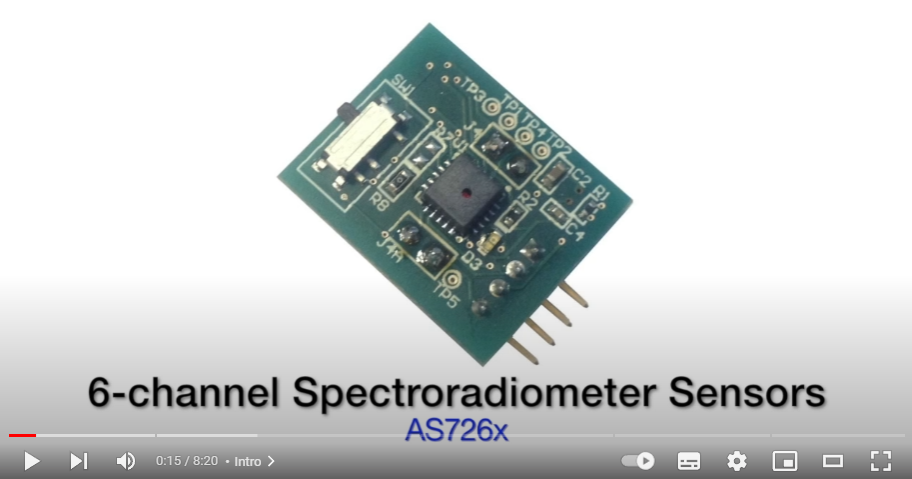
\includegraphics{images/youtube_ams_as7262.png}

}

\caption{ams Spectral ID iSPI Eval Kit}

\end{figure}%

\begin{longtable}[]{@{}
  >{\raggedright\arraybackslash}p{(\columnwidth - 2\tabcolsep) * \real{0.1429}}
  >{\raggedright\arraybackslash}p{(\columnwidth - 2\tabcolsep) * \real{0.8571}}@{}}
\toprule\noalign{}
\begin{minipage}[b]{\linewidth}\raggedright
\textbf{Unterlagen}
\end{minipage} & \begin{minipage}[b]{\linewidth}\raggedright
\end{minipage} \\
\midrule\noalign{}
\endhead
\bottomrule\noalign{}
\endlastfoot
Produkt &
\href{https://shop.pimoroni.com/products/as7262-6-channel-spectral-sensor-spectrometer-breakout}{AS7262
Breakout} \\
Datenblatt &
\href{https://ams.com/documents/20143/36005/AS7262_DS000486_5-00.pdf}{AS7262} \\
GitHub &
\href{https://github.com/pimoroni/as7262-python}{as7262-python} \\
Video & \href{https://www.youtube.com/watch?v=KKyHxXyaVPM}{ams Spectral
ID iSPI Eval Kit} \\
\end{longtable}

\section*{Spektrometer}\label{spektrometer}
\addcontentsline{toc}{section}{Spektrometer}

\markright{Spektrometer}

Spektrometer, sind Sensoren, die das Licht auf einzelne Bänder der
Wellenlänge (in Nanometer nm) messen. Für das menschliche Auge wird das
sichtbare Spektrum zwischen 360nm bis 830nm angegeben, wobei sich der
Bereich unter optimalen Bedingungen in UV und NIR erstrecken kann
(Sliney 2016).

Auf kleinen Chip verbaute Spektralsensoren ermöglichen zahlreiche neue
Anwendungen, die früher mit grossen Spektroskopen durchgeführt wurden.
Die Spektralsensorsysteme finden Anwendung wie Farbbestimmung,
Authentifizierung und Spektralanalyse von Substanzen, Materialien,
Lebensmitteln und Flüssigkeiten und werden in den Bereichen von
Konsumgütern, Industrie und Medizin eingesetzt.

Ein Multispektralsensor liefert die Antwort auf die Frage, ob eine
orangefarbene Probe eine Mischung aus Rot und Gelb oder ein reines
Orange ist. Multispektralsensoren teilen das gewählte Spektrum in
Spektralkanäle auf (siehe Abbildung~\ref{fig-as7262}) und sind so
angeordnet, dass die Spektralkanäle kontinuierlich gut abgedeckt sind.
Die Messung erfolgt im sichtbaren Bereich radiometrisch (Jensen 2020).
Das heißt, der Sensor misst die spektrale Leistungsverteilung der
Messung.

\section*{\texorpdfstring{AS7262
Multispektralsensor\index{AS7262}}{AS7262 Multispektralsensor}}\label{as7262-multispektralsensor}
\addcontentsline{toc}{section}{AS7262 Multispektralsensor\index{AS7262}}

\markright{AS7262 Multispektralsensor\index{AS7262}}

Der AS7262 ist ein sehr kompakter Multispektralsensor, der über 6
Spektralkanäle im sichtbaren Bereich misst. Der Sensor eignet sich für
spektroskopische Messungen wie \emph{Farbmessung, Absorption,
Bestrahlungsstärke, Reflexion} und \emph{Transmission}. Der Sensor ist
auf einem Breakout Board verbaut und kann über die I2C Schnittstelle mit
dem Raspberry Pi verbunden werden, zusätzlich sind zwei LEDs verbaut,
die den Messbereich für Messungen beleuchten können.

AS7262 - 6-Kanal Spektral Sensor (Abbildung~\ref{fig-as7262})

\begin{itemize}
\tightlist
\item
  6 Spektralkanäle (450, 500, 550, 570, 600, 650nm)
\item
  2 on-board Beleuchtungs-LEDs
\item
  I2C interface~(address: 0x49)
\item
  Python Library
\item
  werkseitig kalibriert
\end{itemize}

\begin{figure}

\centering{

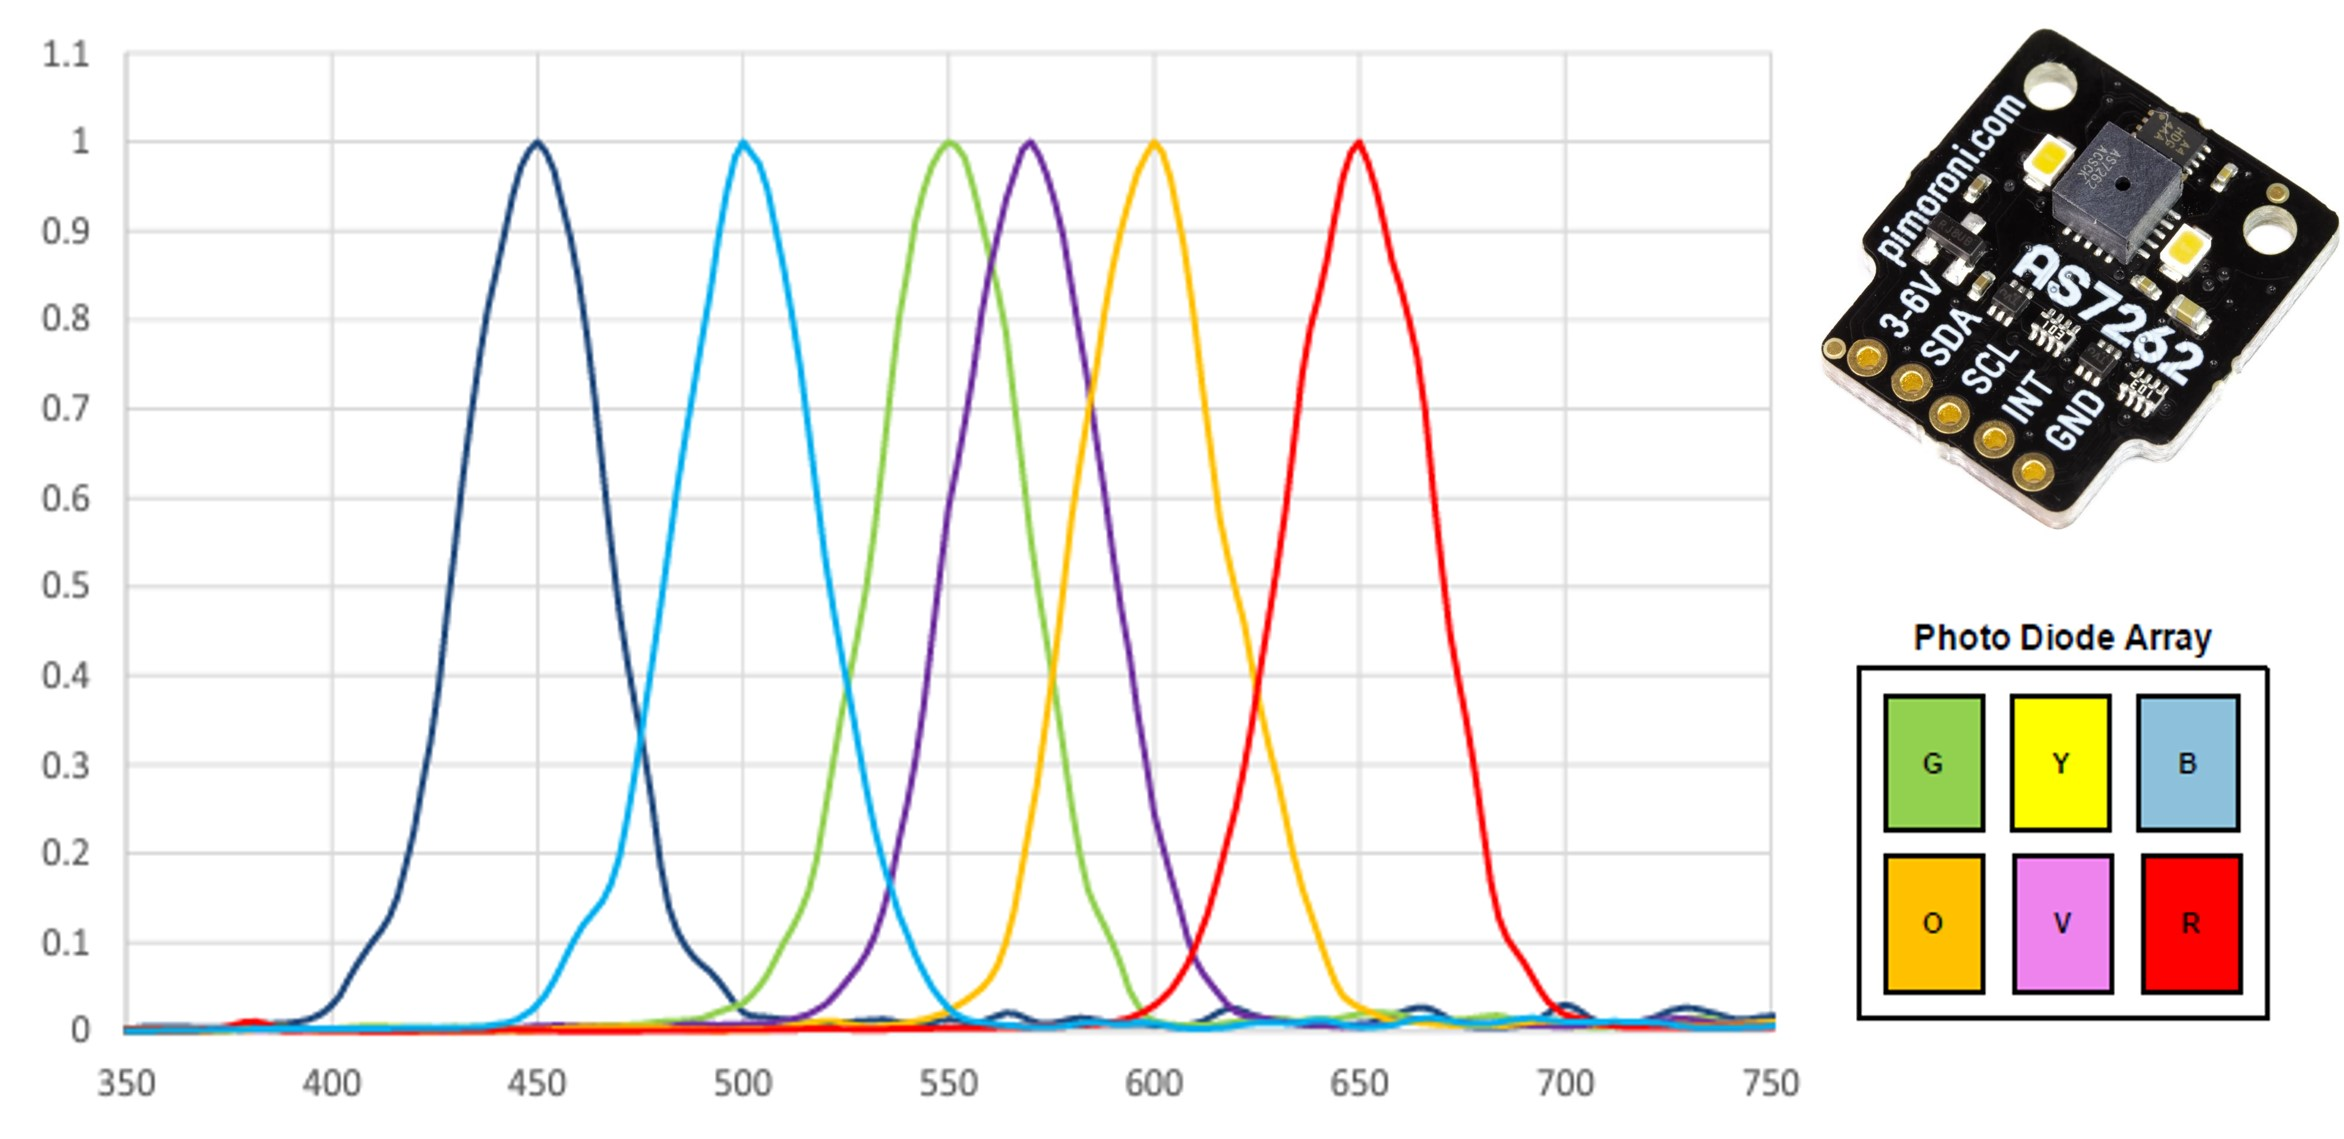
\includegraphics{images/AS7262_wide.jpg}

}

\caption{\label{fig-as7262}links: Spektrale Sensitivität des AS7262,
oben: AS7262 Breakout von Pimoroni, unten: AS7262 Photodioden Array}

\end{figure}%

\section*{Übungsaufbau}\label{uxfcbungsaufbau-1}
\addcontentsline{toc}{section}{Übungsaufbau}

\markright{Übungsaufbau}

\begin{itemize}
\tightlist
\item
  Schliesse den Raspberry Pi an Monitor, Keyboard und Maus an oder
  verbinde Dich mit diesem über SSH (und SFTP).
\item
  Erstelle auf dem Raspberry Pi im \texttt{Documents} Ordner einen neuen
  Ordner \texttt{AS7262}, in welchem Du Änderungen und neue Dateien für
  diese Übung speichern kannst.
\item
  Schliesse den Sensor \textbf{AS7262} an den Raspberry Pi über die
  Breakout Garden \textbf{I2C} Schnittstelle korrekt an (siehe
  \href{E01_Luftqualitaet.qmd}{E01 Luftqualität}), so dass die
  Beschriftung der Anschlüsse am Sensor und bei der Schnittstelle
  übereinstimmen.
\item
  Kontrolliere mit dem Befehl \texttt{i2cdetect\ -y\ 1} ob der Raspberry
  Pi mit dem Sensor verbunden ist. Der Sensor sollte auf der Adresse
  \texttt{0x49} erkannt werden.
\item
  Kontrolliere, ob die Library \texttt{as7262} installiert ist mit
  \texttt{python\ -c\ "import\ as7262"}. Installiere die Library mit
  \texttt{sudo\ pip3\ install\ as7262} falls sie nicht installiert ist.
\end{itemize}

Wechsle in den Ordner \emph{Documents} und kopiere mit folgenden
Befehlen die Library auf Deinen Raspberry Pi.

\begin{Shaded}
\begin{Highlighting}[]
\BuiltInTok{cd}\NormalTok{ Documents}
\FunctionTok{git}\NormalTok{ clone https://github.com/pimoroni/as7262{-}python}
\BuiltInTok{cd}\NormalTok{ as7262{-}python/examples}
\end{Highlighting}
\end{Shaded}

\section*{Aufgabe 1: Spektralmessungen
durchführen}\label{aufgabe-1-spektralmessungen-durchfuxfchren}
\addcontentsline{toc}{section}{Aufgabe 1: Spektralmessungen durchführen}

\markright{Aufgabe 1: Spektralmessungen durchführen}

Teste das Beispiel \texttt{spectrum.py} im Ordner \emph{examples}.
Dieses Beispiel gibt die Messungen der einzelnen Spektralkänale aus.

Startet das Script mit \texttt{python3\ spectrum.py}. Mit
\texttt{Ctrl+c} kann das Script wieder gestopppt werden. Die Ausgabe
sollte in etwa so aussehen (gekürzt):

\begin{Shaded}
\begin{Highlighting}[]
\ExtensionTok{python3}\NormalTok{ spectrum.py}
\ExtensionTok{Orange:}\NormalTok{ 30.22943878173828}
\ExtensionTok{Red:}\NormalTok{    14.262250900268555}
\ExtensionTok{Orange:}\NormalTok{ 22.67207908630371}
\ExtensionTok{Yellow:}\NormalTok{ 14.271308898925781}
\ExtensionTok{Green:}\NormalTok{  13.56598949432373}
\ExtensionTok{Blue:}\NormalTok{   6.527451515197754}
\ExtensionTok{Violet:}\NormalTok{ 7.2663960456848145}
\end{Highlighting}
\end{Shaded}

Folgendes Code Snippet zeigt eine gekürzte Version des
\texttt{spectrum.py} Python Beispiels für die Ausgabe der
Spektralmessungen der 6 Kanäle:

\phantomsection\label{annotated-cell-13}%
\begin{Shaded}
\begin{Highlighting}[]
\CommentTok{\#!/usr/bin/env python}
\ImportTok{from}\NormalTok{ as7262 }\ImportTok{import}\NormalTok{ AS7262}
\NormalTok{as7262 }\OperatorTok{=}\NormalTok{ AS7262()}
\NormalTok{as7262.set\_gain(}\DecValTok{64}\NormalTok{) }\hspace*{\fill}\NormalTok{\circled{1}}
\NormalTok{as7262.set\_integration\_time(}\FloatTok{17.857}\NormalTok{) }
\NormalTok{as7262.set\_measurement\_mode(}\DecValTok{2}\NormalTok{) }
\NormalTok{as7262.set\_illumination\_led(}\DecValTok{1}\NormalTok{) }

\ControlFlowTok{try}\NormalTok{:}
    \ControlFlowTok{while} \VariableTok{True}\NormalTok{:}
\NormalTok{        values }\OperatorTok{=}\NormalTok{ as7262.get\_calibrated\_values() }\hspace*{\fill}\NormalTok{\circled{2}}
        \BuiltInTok{print}\NormalTok{(}\StringTok{"""}
\StringTok{Red:    }\SpecialCharTok{\{\}}
\StringTok{Orange: }\SpecialCharTok{\{\}}
\StringTok{Yellow: }\SpecialCharTok{\{\}}
\StringTok{Green:  }\SpecialCharTok{\{\}}
\StringTok{Blue:   }\SpecialCharTok{\{\}}
\StringTok{Violet: }\SpecialCharTok{\{\}}\StringTok{"""}\NormalTok{.}\BuiltInTok{format}\NormalTok{(}\OperatorTok{*}\NormalTok{values))}

\ControlFlowTok{except} \PreprocessorTok{KeyboardInterrupt}\NormalTok{:}
\NormalTok{    as7262.set\_measurement\_mode(}\DecValTok{3}\NormalTok{)}
\NormalTok{    as7262.set\_illumination\_led(}\DecValTok{0}\NormalTok{)}
\end{Highlighting}
\end{Shaded}

\begin{description}
\tightlist
\item[\circled{1}]
Sensor konfigurieren, setzen des Gains, der Integrationszeit, des
Messmodus und der Beleuchtungs LED
\item[\circled{2}]
Kalibrierte Messwerte auslesen und darstellen
\end{description}

\begin{boxtitle}{Excercise}{colPrimary}

\textbf{AS7262 Messwerte interpretieren}\\
Führt einige Messungen mit unterschiedlichen Lichtquellen und
Materialien durch und notiert Euch die Messwerte. Was beobachtet Ihr?

\begin{itemize}
\tightlist
\item
  Messung mit Tageslicht
\item
  Messung mit LED-Taschenlampe des Smartphones
\item
  Messung mit LED-Taschenlampe und Farbfilter (Mäppli)
\item
  Messung mit weissem Papier
\end{itemize}

\end{boxtitle}

\section*{Aufgabe 2: Spektralmessungen mit Visualisierung in der
Konsole}\label{aufgabe-2-spektralmessungen-mit-visualisierung-in-der-konsole}
\addcontentsline{toc}{section}{Aufgabe 2: Spektralmessungen mit
Visualisierung in der Konsole}

\markright{Aufgabe 2: Spektralmessungen mit Visualisierung in der
Konsole}

Das Beispiel \texttt{bargraph.py} zeigt die Messwerte der Spektralkanäle
in einem Balkendiagramm an. Die Messwerte werden in der Konsole
ausgegeben, nach einem Weissabgleich. Der Weissabgleich wird benötigt
damit der Sensoren die Messwerte korrekt in Referenz zu Weiss
interpretiert.

Für diese Aufgabe benötigt Ihr ein weisse Blatt Papier, mit welchem der
Sensor den Weissabgleich durchführt. Dafür hält ihr dieses circa 5cm vor
den Sensor, drückt eine Taste und der Sensor führt den Weissabgleich
durch. Danach könnt Ihr das Papier wieder wegnehmen und die Messungen
durchführen.

\begin{boxtitle}{Excercise}{colPrimary}

\textbf{Verteilung der Spektralkanäle untersuchen}

\begin{itemize}
\tightlist
\item
  Führt verschiedene Messungen durch mit unterschiedlichen Lichtquellen
  und Materialien und interpretiert die Ausgabe des
  \texttt{bargraph.py}.
\item
  Studiert den Code und versucht die Funktionsweise zu verstehen.
\end{itemize}

\end{boxtitle}

\begin{Shaded}
\begin{Highlighting}[]
\ExtensionTok{python3}\NormalTok{ bargraph.py }
\ExtensionTok{Setting}\NormalTok{ white point baseline.}

\ExtensionTok{Hold}\NormalTok{ a white sheet of paper \textasciitilde{}5cm in front of the sensor and press a key...}

\ExtensionTok{Baseline}\NormalTok{ set. Press a key to continue...   }
\end{Highlighting}
\end{Shaded}

\begin{figure}[H]

{\centering 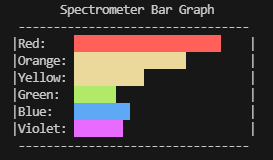
\includegraphics{images/as7262_bargraph.png}

}

\caption{Beispiel Ausgabe von \texttt{bargraph.py} Spectrometer Bar
Graph}

\end{figure}%

\chapter*{E03 Bewegungsmessung}\label{e03-bewegungsmessung}
\addcontentsline{toc}{chapter}{E03 Bewegungsmessung}

\markboth{E03 Bewegungsmessung}{E03 Bewegungsmessung}

Ziel dieser Übung ist es Bewegungsmessung mit inertialen Messeinheiten
(IMU)\index{IMU} über den ICM20948 Bewegungssensor kennen zu lernen und
die Sensordaten auszulesen und testen. Der \emph{ICM20948} ist ein 9DoF
Bewegungssensor, der über eine I2C Schnittstelle mit dem Raspberry Pi
verbunden wird und einer Python Library angesteuert werden kann.

\textbf{Vorbereitung}

\begin{itemize}
\tightlist
\item
  Schaut das Video zur Funktionsweise von MEMS Bewegungssensoren

  \begin{itemize}
  \tightlist
  \item
    Video:
    \href{https://www.youtube.com/embed/eqZgxR6eRjo?si=u28t9yfD4BLPeYGd}{How
    MEMS Accelerometer Gyroscope Magnetometer Work} (bis Minute 2:50),
    sowie folgendes
  \item
    Video:
    \href{https://www.youtube.com/embed/swCTbz5sIQM?si=Uga2sPKfiQW7EO6z}{Bosch
    Funktionsprinzip eines Beschleunigungssensors}
  \end{itemize}
\item
  Studiere das Datenblatt zum ICM-20948 (InvenSense 2021)

  \begin{itemize}
  \tightlist
  \item
    In welchen Temperaturbereichen kann der Sensor eingesetzt werden?
  \end{itemize}
\item
  Installiere auf deinem Smartphone die Applikation
  \emph{\href{https://phyphox.org}{phyphox}} und teste die
  Beschleunigungssensoren deines Smartphones.
\end{itemize}

\begin{figure}[H]

{\centering 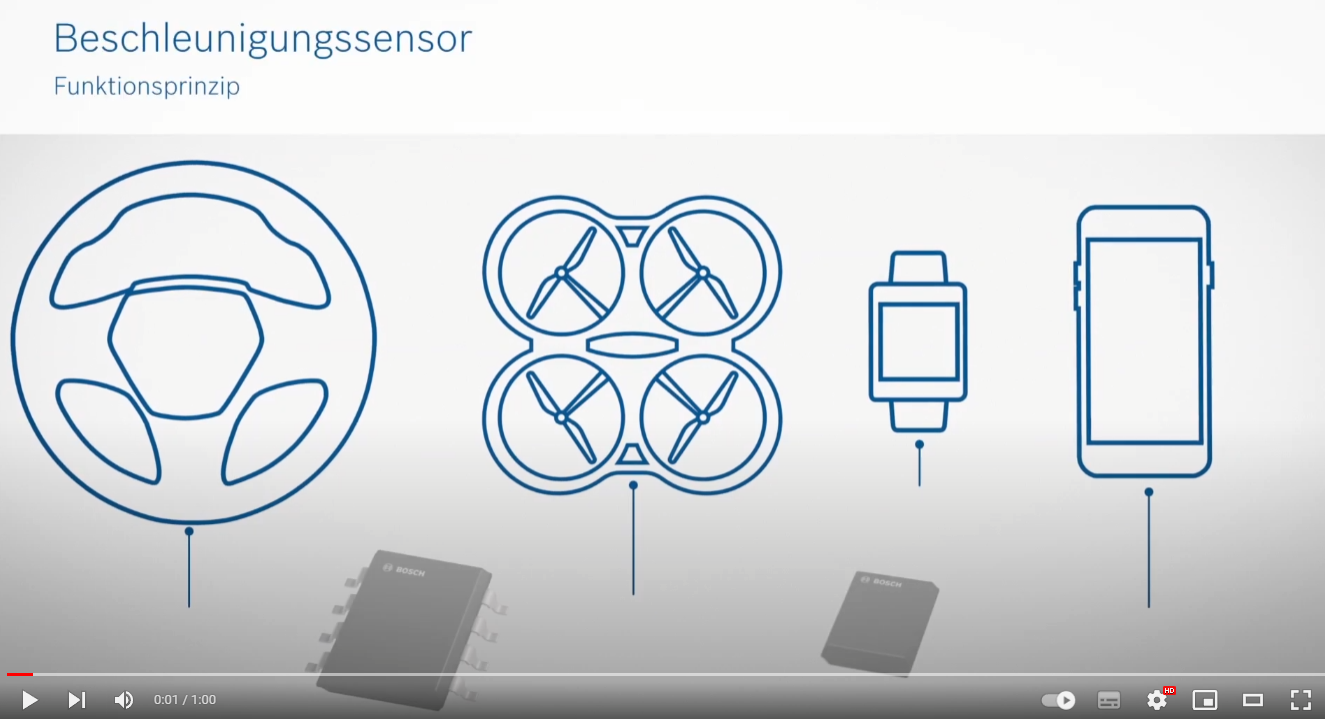
\includegraphics{images/youtube_bosch_beschleunigungssensor.png}

}

\caption{How MEMS Accelerometer Gyroscope Magnetometer Work \& Arduino
Tutorial}

\end{figure}%

\begin{longtable}[]{@{}
  >{\raggedright\arraybackslash}p{(\columnwidth - 2\tabcolsep) * \real{0.1429}}
  >{\raggedright\arraybackslash}p{(\columnwidth - 2\tabcolsep) * \real{0.8571}}@{}}
\toprule\noalign{}
\begin{minipage}[b]{\linewidth}\raggedright
\textbf{Unterlagen}
\end{minipage} & \begin{minipage}[b]{\linewidth}\raggedright
\end{minipage} \\
\midrule\noalign{}
\endhead
\bottomrule\noalign{}
\endlastfoot
Produkt & \href{https://shop.pimoroni.com/products/icm20948}{ICM20948
Breakout} \\
Datenblatt &
\href{https://www.invensense.com/wp-content/uploads/2016/06/DS-000189-ICM-20948-v1.3.pdf}{ICM
20948} \\
GitHub &
\href{https://github.com/pimoroni/icm20948-python}{icm20948-python} \\
\end{longtable}

\section*{Beschleunigungssensoren
IMU}\label{beschleunigungssensoren-imu}
\addcontentsline{toc}{section}{Beschleunigungssensoren IMU}

\markright{Beschleunigungssensoren IMU}

Beschleunigungssensoren, oder inertiale Messeinheit (inertial
measurement unit IMU) messen die Beschleunigung von Objekten mit dem
Messprinzip der Trägheit und erfassen die Kraft die auf die Masse des
Objekt wirkt, wenn dieses beschleunigt wird.

Für die Erfassung der sechs kinematischen Freiheitsgrade werden drei
Achsen der Beschleunigung (Accelerometer) und drei Achsen der Rotation
(Gyroskop) gemessen, die die Beschleunigungsmessung und
Winkelgeschwindigkeit der Drehraten ausgeben. Für die Erfassung der
Orientierung im Raum wird ein Magnetometer eingesetzt, welches die
Ausrichtung des Objekts im Magnetfeld der Erde misst, um die Ausrichtung
im Raum zu bestimmen. Wenn alle drei Sensoren kombiniert werden, spricht
man von 9DoF Motion Sensoren, der neun Freiheitsgrade (9 Degrees of
Freedom) misst.

Beschleunigungssensoren werden in vielen Anwendungen eingesetzt, wie
z.B. in der Automobilindustrie (Auslösen von Airbags), der Luft- und
Raumfahrt, der Medizintechnik (Beschleunigungssensoren in
Herzschrittmachern) und der Unterhaltungselektronik (Smartphones für die
Ausrichtung des Bildschirms).

\section*{\texorpdfstring{ICM20948 9DoF Motion
Sensor\index{ICM20948}}{ICM20948 9DoF Motion Sensor}}\label{icm20948-9dof-motion-sensor}
\addcontentsline{toc}{section}{ICM20948 9DoF Motion
Sensor\index{ICM20948}}

\markright{ICM20948 9DoF Motion Sensor\index{ICM20948}}

Der ICM-20948 von
\href{https://invensense.tdk.com/products/motion-tracking/9-axis/icm-20948}{TDK
InvenSense} (Abbildung~\ref{fig-icm20948}) ist ein 9-Achsen MEMS
Bewegungssensor, mit einem 3-Achsen Gyroskop, einem 3-Achsen
Beschleunigungssensor und einem 3-Achsen Magnetometer und sehr geringem
Stromverbrauch. Er enthält zwei Chip, einen für die Bewegungsmessung mit
Gyroskop und Beschleunigungssensor und einen zweiten für das
Magnetometer.

MEMS\index{MEMS} sind mikroelektromechanische Systeme, die aus
mikroskopisch kleinen mechanischen und elektrischen Komponenten
bestehen. Diese werden meist aus Silicium hergestellt und sind im Falle
von Beschleunigungssensoren sehr kleine Massen, die sich bei
Beschleunigung bewegen und die Änderung der elektrischen Kapazität
messen.

9DoF Motion Accelero-, Gyro-, Magnetometer

\begin{itemize}
\tightlist
\item
  ±2/±4/±8/±16 g 3-axis accelerometer
\item
  ±250/±500/±1000/±2000 DPS (degrees per second) 3-axis gyroscope
\item
  3-axis compass with wide range up to ±4900 μT
\item
  Python, C Library
\item
  I2C interface~(address: 0x68 or0x69)
\item
  Qw/ST (Qwiic/STEMMA QT) connector
\item
  I2C interface (address 0x68/0x69 (cut trace))
\end{itemize}

\begin{figure}

\centering{

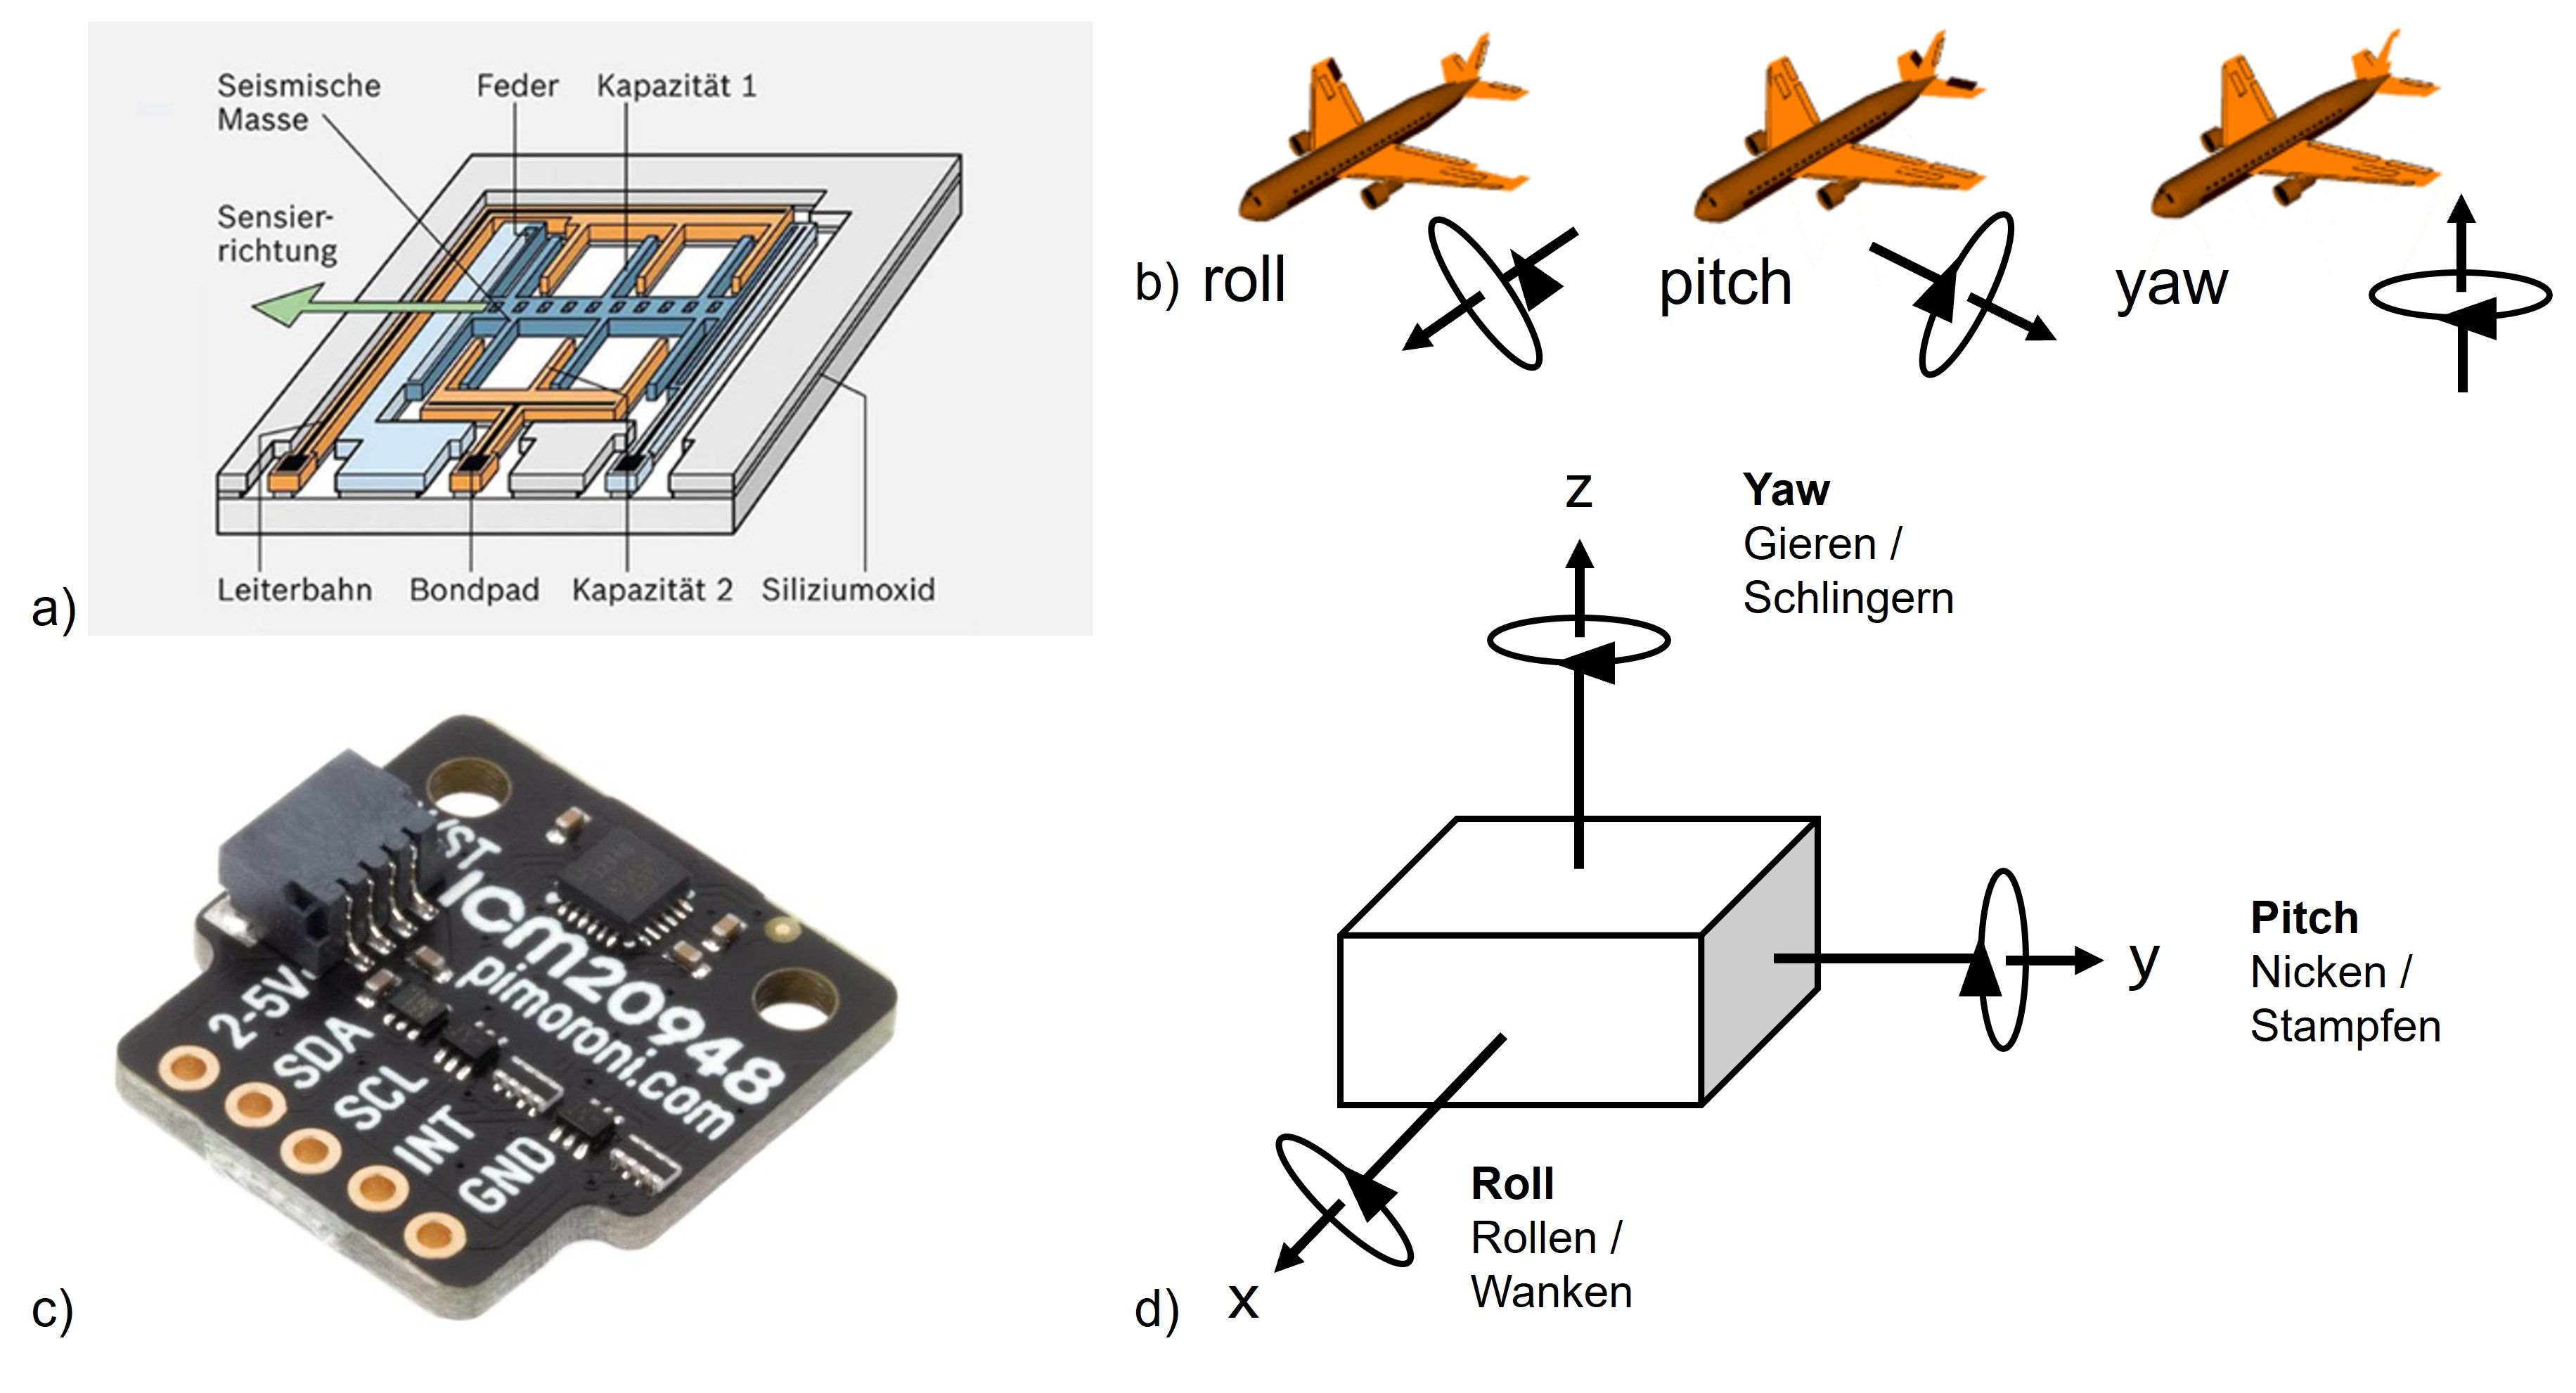
\includegraphics{images/ICM20948_wide.jpg}

}

\caption{\label{fig-icm20948}a) schematische Darstellung eines MEMS
Beschleunigungssensors Quelle: Bosch, b) raw, pitch, roll bei
Flugzeugen, c) ICM-20948 Breakout von Pimoroni, d) Orientierung von IMU
Sensoren.}

\end{figure}%

\section*{Übungsaufbau}\label{uxfcbungsaufbau-2}
\addcontentsline{toc}{section}{Übungsaufbau}

\markright{Übungsaufbau}

\begin{itemize}
\tightlist
\item
  Schliesse den Raspberry Pi an Monitor, Keyboard und Maus an oder
  verbinde Dich mit diesem über SSH (und SFTP).
\item
  Erstelle auf dem Raspberry Pi im \texttt{Documents} Ordner einen neuen
  Ordner \texttt{ICM20948}, in welchem Du Änderungen und neue Dateien
  für diese Übung speichern kannst.
\item
  Schliesse den Sensor \textbf{ICM20948} an den Raspberry Pi über die
  Breakout Garden \textbf{I2C} Schnittstelle korrekt an (siehe
  \href{E01_Luftqualitaet.qmd}{E01 Luftqualität}), so dass die
  Beschriftung der Anschlüsse am Sensor und bei der Schnittstelle
  übereinstimmen.
\item
  Kontrolliere mit dem Befehl \texttt{i2cdetect\ -y\ 1} ob der Raspberry
  Pi mit dem Sensor verbunden ist. Der Sensor sollte auf der Adresse
  \texttt{0x68} erkannt werden.
\item
  Kontrolliere, ob die Library \texttt{icm20948} installiert ist mit
  \texttt{python\ -c\ "import\ icm20948"}. Installiere die Library mit
  \texttt{sudo\ pip3\ install\ icm20948} falls sie nicht installiert
  ist.
\end{itemize}

Wechsle in den Ordner \emph{Documents} und kopiere mit folgenden
Befehlen die Library auf Deinen Raspberry Pi.

\begin{Shaded}
\begin{Highlighting}[]
\BuiltInTok{cd}\NormalTok{ Documents}
\FunctionTok{git}\NormalTok{ clone https://github.com/pimoroni/icm20948{-}python}
\BuiltInTok{cd}\NormalTok{ icm20948{-}python/examples}
\end{Highlighting}
\end{Shaded}

\section*{Aufgabe 1: Bewegungsmessungen
durchführen}\label{aufgabe-1-bewegungsmessungen-durchfuxfchren}
\addcontentsline{toc}{section}{Aufgabe 1: Bewegungsmessungen
durchführen}

\markright{Aufgabe 1: Bewegungsmessungen durchführen}

Teste das Beispiel \texttt{read-all.py} im Ordner \emph{examples}.
Dieses Beispiel gibt die Messungen der einzelnen Bewegungsmessungen aus,
der Beschleunigung, Winkelgeschwindigkeit und Orientierung mit dem
Accelerometer, Gyrometer und Magnetometer.

Startet das Script mit \texttt{python3\ read-all.py}. Mit
\texttt{Ctrl+c} kann das Script wieder gestopppt werden. Die Ausgabe
sollte in etwa so aussehen (gekürzt):

\begin{Shaded}
\begin{Highlighting}[]
\ExtensionTok{python3}\NormalTok{ read{-}all.py}
\ExtensionTok{read{-}all.py}
\ExtensionTok{Reads}\NormalTok{ all ranges of movement: accelerometer, gyroscope and compass heading.}
\ExtensionTok{Press}\NormalTok{ Ctrl+C to exit!}

\ExtensionTok{Accel:}\NormalTok{ 01.01 }\AttributeTok{{-}0.02}\NormalTok{ 00.01}
\ExtensionTok{Gyro:}  \AttributeTok{{-}0.42}\NormalTok{ 01.73 00.01}
\ExtensionTok{Mag:}   \AttributeTok{{-}86.85}\NormalTok{ 57.45 34.05}

\ExtensionTok{Accel:}\NormalTok{ 01.01 }\AttributeTok{{-}0.02}\NormalTok{ 00.02}
\ExtensionTok{Gyro:}  \AttributeTok{{-}0.40}\NormalTok{ 01.50 }\AttributeTok{{-}0.16}
\ExtensionTok{Mag:}   \AttributeTok{{-}85.35}\NormalTok{ 55.50 34.80}
\end{Highlighting}
\end{Shaded}

Folgendes Code Snippet zeigt eine gekürzte Version des
\texttt{read-all.py} Python Beispiels für die Ausgabe der
Beschleunigungsmessung.

\phantomsection\label{annotated-cell-17}%
\begin{Shaded}
\begin{Highlighting}[]
\CommentTok{\#!/usr/bin/env python}
\ImportTok{import}\NormalTok{ time}
\ImportTok{from}\NormalTok{ icm20948 }\ImportTok{import}\NormalTok{ ICM20948}

\NormalTok{imu }\OperatorTok{=}\NormalTok{ ICM20948()}

\ControlFlowTok{while} \VariableTok{True}\NormalTok{:}
\NormalTok{    x, y, z }\OperatorTok{=}\NormalTok{ imu.read\_magnetometer\_data() }\hspace*{\fill}\NormalTok{\circled{1}}
\NormalTok{    ax, ay, az, gx, gy, gz }\OperatorTok{=}\NormalTok{ imu.read\_accelerometer\_gyro\_data() }\hspace*{\fill}\NormalTok{\circled{2}}

    \BuiltInTok{print}\NormalTok{(}\StringTok{""" \# \textless{}3\textgreater{}}
\StringTok{Accel: }\SpecialCharTok{\{:05.2f\}}\StringTok{ }\SpecialCharTok{\{:05.2f\}}\StringTok{ }\SpecialCharTok{\{:05.2f\}}
\StringTok{Gyro:  }\SpecialCharTok{\{:05.2f\}}\StringTok{ }\SpecialCharTok{\{:05.2f\}}\StringTok{ }\SpecialCharTok{\{:05.2f\}}
\StringTok{Mag:   }\SpecialCharTok{\{:05.2f\}}\StringTok{ }\SpecialCharTok{\{:05.2f\}}\StringTok{ }\SpecialCharTok{\{:05.2f\}}\StringTok{"""}\NormalTok{.}\BuiltInTok{format}\NormalTok{(}
\NormalTok{        ax, ay, az, gx, gy, gz, x, y, z}
\NormalTok{        ))}

\NormalTok{    time.sleep(}\FloatTok{0.25}\NormalTok{) }\hspace*{\fill}\NormalTok{\circled{4}}
\end{Highlighting}
\end{Shaded}

\begin{description}
\tightlist
\item[\circled{1}]
Auslesen des Magnetometers (x,y,z)
\item[\circled{2}]
Auslesen des Accelerometers (ax,ay,az) und Gyrometers (gx,gy,gz)
\item[\circled{3}]
Messwerte auf der Konsole ausgeben
\item[\circled{4}]
Warten 0.25 Sekunden (damit die Ausgabe nicht zu schnell ist)
\end{description}

\begin{boxtitle}{Excercise}{colPrimary}

\textbf{Bewegungsmessung}\\

\begin{itemize}
\tightlist
\item
  Führe das Beispiel \texttt{read-all.py} aus und beobachte die
  Messwerte.
\item
  Versuche den Sensor jeweils leicht in eine Richtung zu bewegen, zu
  drehen, zu kippen und beobachte die Messwerte.
\item
  Versuche den Sensor zu leicht zu schütteln und beobachte die
  Messwerte.
\item
  Vergleiche die Messwerte mit den Messwerten deines Smartphones mit der
  App \emph{phyphox}.
\item
  Versucht zu eruieren wie die Achsen orientiert sind und vergleicht mit
  anderen Gruppen.
\item
  Schreibe die Messwerte in eine Datei und visualisiere diese mit einem
  Plot, modifiziere dazu das Beispiel \texttt{read-all.py} und speichere
  die Datei als \texttt{read-csv.py}, so dass die Messungen zeilenweise
  mit einem Separator gespeichert werden. Ausgaben aus einem Plot können
  mit dem Befehl
  \texttt{python3\ read-csv.py\ \textgreater{}\ imu\_horizontal.csv} in
  eine Datei geschrieben werden. Nun könnt ihr verschiedene Versuche mit
  der IMU durchführen und in einer Datei speichern. Die Datei könnt ihr
  beispielsweise mit \emph{LibreOffice Calc} oder \emph{Excel} öffnen
  und die Daten visualisieren.
\end{itemize}

\end{boxtitle}

\begin{solution}
Die Datei \texttt{read-csv.py} mit den Messwerten mit Semikolon als
Separator:

\begin{Shaded}
\begin{Highlighting}[]
\CommentTok{\#!/usr/bin/env python}
\ImportTok{import}\NormalTok{ time}
\ImportTok{from}\NormalTok{ icm20948 }\ImportTok{import}\NormalTok{ ICM20948}
\BuiltInTok{print}\NormalTok{(}\StringTok{"ax; ay; az; gx; gy; gz; x; y; z"}\NormalTok{)}
\NormalTok{imu }\OperatorTok{=}\NormalTok{ ICM20948()}

\ControlFlowTok{while} \VariableTok{True}\NormalTok{:}
\NormalTok{    x, y, z }\OperatorTok{=}\NormalTok{ imu.read\_magnetometer\_data()}
\NormalTok{    ax, ay, az, gx, gy, gz }\OperatorTok{=}\NormalTok{ imu.read\_accelerometer\_gyro\_data()}
    \BuiltInTok{print}\NormalTok{(}\StringTok{"""}\SpecialCharTok{\{:05.2f\}}\StringTok{; }\SpecialCharTok{\{:05.2f\}}\StringTok{; }\SpecialCharTok{\{:05.2f\}}\StringTok{; }\SpecialCharTok{\{:05.2f\}}\StringTok{; }\SpecialCharTok{\{:05.2f\}}\StringTok{; }\SpecialCharTok{\{:05.2f\}}\StringTok{; }\SpecialCharTok{\{:05.2f\}}\StringTok{; }\SpecialCharTok{\{:05.2f\}}\StringTok{; }\SpecialCharTok{\{:05.2f\}}\StringTok{"""}\NormalTok{.}\BuiltInTok{format}\NormalTok{(}
\NormalTok{        ax, ay, az, gx, gy, gz, x, y, z ))}
\NormalTok{    time.sleep(}\FloatTok{0.25}\NormalTok{)}
\end{Highlighting}
\end{Shaded}

\end{solution}

\section*{Aufgabe 2: Magnetometer}\label{aufgabe-2-magnetometer}
\addcontentsline{toc}{section}{Aufgabe 2: Magnetometer}

\markright{Aufgabe 2: Magnetometer}

Das Beispiel \texttt{bargraph.py} zeigt die Messwerte des Magnetometers
in einem Balkendiagramm an und zeigt die Orientierung des Sensors an je
nach dem über welche Achse gemessen wird. Der Befehl
\texttt{python3\ bargraph.py\ -\/-help} zeigt die Optionen des Skripts
an.

Die Ausgabe sollte für die Option \texttt{-\/-graph} in etwa so
aussehen:

\begin{Shaded}
\begin{Highlighting}[]
\ExtensionTok{python3}\NormalTok{ bargraph.py }\AttributeTok{{-}{-}graph}
\ExtensionTok{bargraph.py} \AttributeTok{{-}}\NormalTok{ Convert raw values to heading}

\ExtensionTok{Rotate}\NormalTok{ the sensor through 360 degrees to calibrate.}

\ExtensionTok{Press}\NormalTok{ Ctrl+C to exit!}

\ExtensionTok{043.5}\NormalTok{ █████████████                                                                                                     }
\end{Highlighting}
\end{Shaded}

\begin{boxtitle}{Excercise}{colPrimary}

\textbf{Bar graph}

\begin{itemize}
\tightlist
\item
  Kalibriere den Sensor und vergleiche die Orientierung des Sensors mit
  den Himmelsrichtungen
\item
  Vergleiche die Ausgaben auch mit der Orientierung des Smartphones und
  den Messwerten der App \emph{phyphox}.
\item
  Studiert den Code und versucht die Funktionsweise zu verstehen.
\end{itemize}

\end{boxtitle}

\chapter*{E04 Distanzmessung}\label{e04-distanzmessung}
\addcontentsline{toc}{chapter}{E04 Distanzmessung}

\markboth{E04 Distanzmessung}{E04 Distanzmessung}

Ziel dieser Übung ist es Distanzmessungen mit dem VL53L5CX Sensor kennen
zu lernen und die Sensordaten auszulesen und testen. Der \emph{VL53L5CX}
ist ein 8x8 Time of Flight (ToF) Array Sensor, der über eine I2C
Schnittstelle mit dem Raspberry Pi verbunden wird und einer Python
Library angesteuert werden kann.

\textbf{Vorbereitung}

\begin{itemize}
\tightlist
\item
  Schaut folgende von Video von Adafruit Industries zur Funktionsweise
  des VL53L5CX Sensors an:
  \href{https://www.youtube.com/embed/nf527vcKRSE?si=Q2Wm_pS2O1n99-ha}{EYE
  ON NPI - ST VL53L5CX Time-of-Flight Ranging Sensor}
\item
  Studiere das Datenblatt zum VL53L5CX (STMicroelectronics 2021), sowie
  die \emph{Application Note} (STMicroelectronics 2023)

  \begin{itemize}
  \tightlist
  \item
    In welchen Temperaturbereichen kann der Sensor eingesetzt werden?
  \item
    Welches ist die höchste Abtastrate für die Distanzfeldmessungen?
  \item
    Was sind Anwendungsgebiete für diesen Sensor?
  \end{itemize}
\end{itemize}

\begin{figure}[H]

{\centering 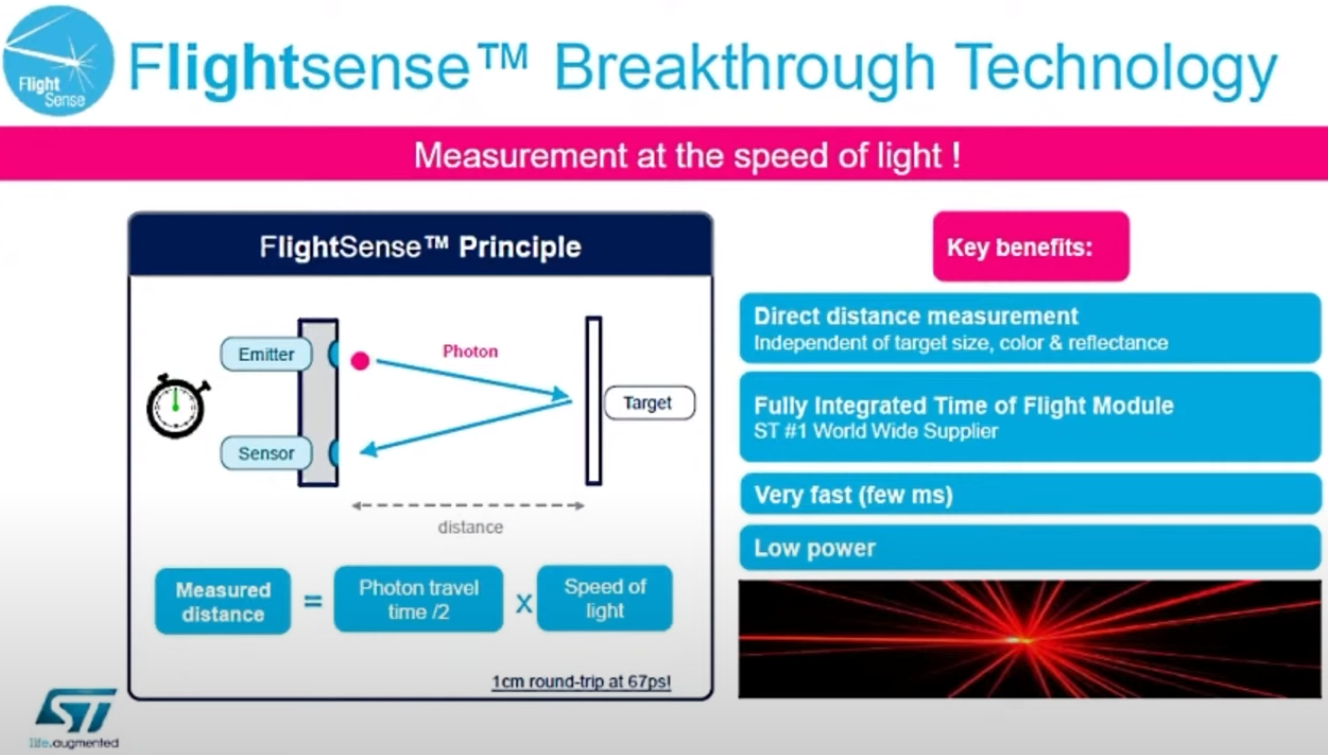
\includegraphics{images/youtube_adafruit_VL53L5CX.png}

}

\caption{Adafruit - EYE ON NPI - ST VL53L5CX Time-of-Flight Ranging
Sensor}

\end{figure}%

\begin{longtable}[]{@{}
  >{\raggedright\arraybackslash}p{(\columnwidth - 2\tabcolsep) * \real{0.1429}}
  >{\raggedright\arraybackslash}p{(\columnwidth - 2\tabcolsep) * \real{0.8571}}@{}}
\toprule\noalign{}
\begin{minipage}[b]{\linewidth}\raggedright
\textbf{Unterlagen}
\end{minipage} & \begin{minipage}[b]{\linewidth}\raggedright
\end{minipage} \\
\midrule\noalign{}
\endhead
\bottomrule\noalign{}
\endlastfoot
Produkt &
\href{https://shop.pimoroni.com/products/vl53l5cx-time-of-flight-tof-sensor-breakout}{VL53L5CX
Breakout} \\
Datenblatt &
\href{https://cdn.shopify.com/s/files/1/0174/1800/files/vl53l5cx.pdf}{VL53L5CX} \\
GitHub &
\href{https://github.com/pimoroni/vl53l5cx-python}{vl53l5cx-python} \\
\end{longtable}

\section*{\texorpdfstring{VL53L5CX 8x8 Time of Flight (ToF) Array
Sensor\index{VL53L5CX}}{VL53L5CX 8x8 Time of Flight (ToF) Array Sensor}}\label{vl53l5cx-8x8-time-of-flight-tof-array-sensor}
\addcontentsline{toc}{section}{VL53L5CX 8x8 Time of Flight (ToF) Array
Sensor\index{VL53L5CX}}

\markright{VL53L5CX 8x8 Time of Flight (ToF) Array
Sensor\index{VL53L5CX}}

Der VL53L5CX ist hochentwickelter Distanzsensor mit einer
8x8-Multizonenmessung und einem großen Sichtfeld, ideal für Roboter und
fortschrittliche Bewegungserkennung. Der mit die Entfernung mit Time of
Flight (ToF), also mit der Laufzeit von Licht, indem er einen
Infrarotlaser mit geringer Leisten auf ein Ziel schickt und die Zeit
misst, die das Licht benötigt, um zurückzukehren.

Dieser Sensor hat eine hohe Genauigkeit und Abtastfrequenz (bis zu 60
Hz) und einen großen Erfassungsbereich (von 2 cm bis 4 m). Besonders
interessant ist, dass der Sensor nicht nur eine Messung durchführt,
sondern eine 8x8 Matrix mit Messwerten zurückgibt. Das bedeutet, das
Bewegungen aus bestimmten Richtungen erkannt werden können oder der
Sensor benutzt werden kann um Kollisionen zu vermeiden oder Objekte zu
verfolgen ohne dass mehrere Sensoren benötigt werden.

VL53L5CX 8x8 Time of Flight (ToF) Array Sensor Breakout

\begin{itemize}
\tightlist
\item
  8x8 Multizone readings
\item
  Distance 2cm - 4m
\item
  I2C interface, with address: 0x52
\item
  Python, C Library
\end{itemize}

\begin{figure}

\centering{

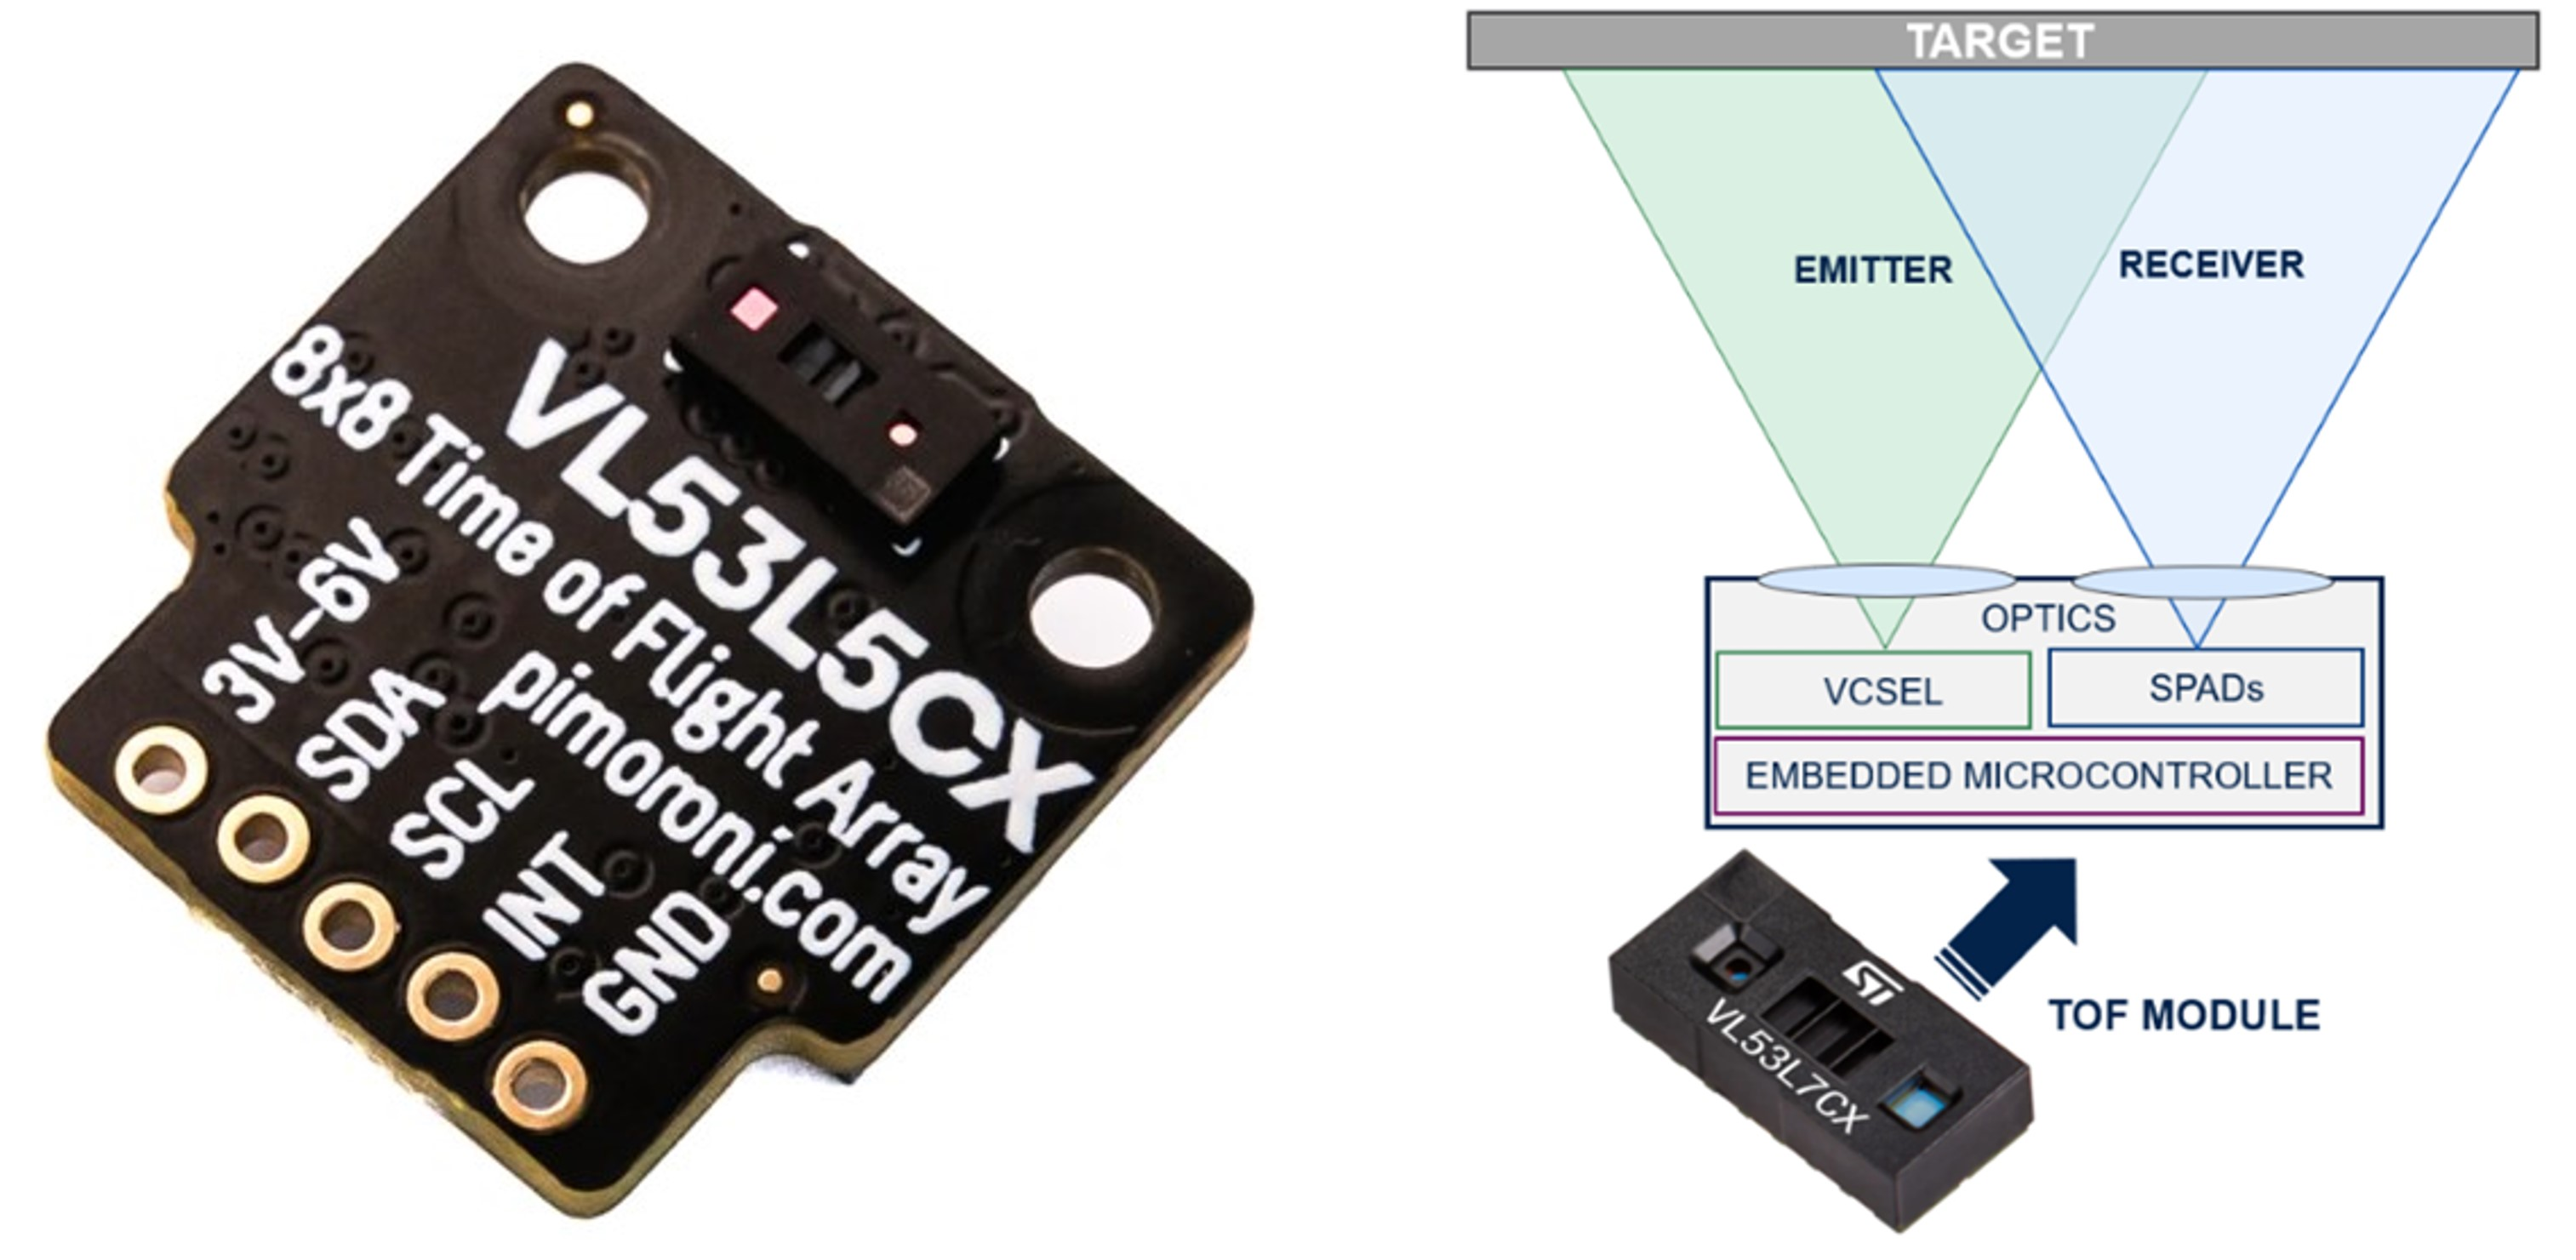
\includegraphics{images/VL53L5CX_wide.jpg}

}

\caption{\label{fig-vl53l5cx}links: VL53L5CX Breakout von Pimoroni,
rechts: schematische Darstellung TOF Moduls Quelle: STMicroelectronics
(2023)}

\end{figure}%

\section*{Übungsaufbau}\label{uxfcbungsaufbau-3}
\addcontentsline{toc}{section}{Übungsaufbau}

\markright{Übungsaufbau}

\begin{itemize}
\tightlist
\item
  Schliesse den Raspberry Pi an Monitor, Keyboard und Maus an oder
  verbinde Dich mit diesem über SSH (und SFTP).
\item
  Erstelle auf dem Raspberry Pi im \texttt{Documents} Ordner einen neuen
  Ordner \texttt{VL53L5CX}, in welchem Du Änderungen und neue Dateien
  für diese Übung speichern kannst.
\item
  Schliesse den Sensor \textbf{VL53L5CX} an den Raspberry Pi über die
  Breakout Garden \textbf{I2C} Schnittstelle korrekt an (siehe
  \href{E01_Luftqualitaet.qmd}{E01 Luftqualität}), so dass die
  Beschriftung der Anschlüsse am Sensor und bei der Schnittstelle
  übereinstimmen.
\item
  Kontrolliere mit dem Befehl \texttt{i2cdetect\ -y\ 1} ob der Raspberry
  Pi mit dem Sensor verbunden ist. Der Sensor sollte auf der Adresse
  \texttt{0x29} erkannt werden.
\item
  Kontrolliere, ob die Library \texttt{vl53l5cx\_ctypes} installiert ist
  mit \texttt{python\ -c\ "import\ vl53l5cx\_ctypes"}. Installiere die
  Library mit \texttt{sudo\ pip3\ install\ vl53l5cx-ctypes} falls sie
  nicht installiert ist.
\end{itemize}

Wechsle in den Ordner \emph{Documents} und kopiere mit folgenden
Befehlen die Library auf Deinen Raspberry Pi.

\begin{Shaded}
\begin{Highlighting}[]
\BuiltInTok{cd}\NormalTok{ Documents}
\FunctionTok{git}\NormalTok{ clone https://github.com/pimoroni/vl53l5cx{-}python}
\BuiltInTok{cd}\NormalTok{ vl53l5cx{-}python/examples}
\end{Highlighting}
\end{Shaded}

\section*{Aufgabe 1: Distanzmessung
Konsole}\label{aufgabe-1-distanzmessung-konsole}
\addcontentsline{toc}{section}{Aufgabe 1: Distanzmessung Konsole}

\markright{Aufgabe 1: Distanzmessung Konsole}

Teste das Beispiel \texttt{test.py} im Ordner \emph{examples}. Dieses
Beispiel liest die Werte der 8x8 Time of Flight Messung aus mit Werten
zu \emph{motion, distance, reflectance} und \emph{status} aus.

\begin{boxtitle}{Hinweis}{colPrimary}

Das Script startet langsam, da die Library jeweils die Firmware beim
Starten lädt.

\end{boxtitle}

Startet das Script mit \texttt{python3\ test.py}. Mit \texttt{Ctrl+c}
kann das Script wieder gestopppt werden. Die Ausgabe sollte in etwa so
aussehen (gekürzt):

\begin{Shaded}
\begin{Highlighting}[]
\ExtensionTok{python3}\NormalTok{ test.py }
\ExtensionTok{Uploading}\NormalTok{ firmware, please wait...}
\ExtensionTok{Done!}
\KeywordTok{[[}\NormalTok{  36   26 2356  }\ErrorTok{543}\ExtensionTok{]}
 \BuiltInTok{[}\NormalTok{  38   62 1943 }\ErrorTok{3847}\ExtensionTok{]}
 \BuiltInTok{[}\NormalTok{  27   68  530 }\ErrorTok{6744}\ExtensionTok{]}
 \BuiltInTok{[}\NormalTok{  14   18   66  }\ErrorTok{458]]} \ExtensionTok{[[1254}\NormalTok{  308  406 2042  365  377  314  237]}
 \ExtensionTok{[1275}\NormalTok{  351  397  413  404  403  354  228]}
 \ExtensionTok{[1297}\NormalTok{  357  375  432  427  422  391  241]}
 \ExtensionTok{[1250}\NormalTok{  348  385  389  415  437  398  315]}
 \ExtensionTok{[1273}\NormalTok{  358  358  385  405  429  400  363]}
 \ExtensionTok{[1238}\NormalTok{  336 2240  368  424  417  379  336]}
 \ExtensionTok{[1262}\NormalTok{  226 2215  180  188  218  202  190]}
 \BuiltInTok{[}\NormalTok{ 108  110  113  }\ErrorTok{117}  \ExtensionTok{116}\NormalTok{  120  120  124]] [[23  1  2 30 11  8 27 41]}
 \ExtensionTok{[16}\NormalTok{  1  3  4  4 17 43 35]}
 \ExtensionTok{[23}\NormalTok{  1  2  6  5 21 58 32]}
 \ExtensionTok{[21}\NormalTok{  1  2  4  6 32 62 52]}
 \ExtensionTok{[27}\NormalTok{  1  3  5  9 36 65 71]}
 \ExtensionTok{[27}\NormalTok{  1 59  5 16 47 52 46]}
 \ExtensionTok{[26}\NormalTok{  1 39  6  9 20 20 21]}
 \ExtensionTok{[13}\NormalTok{ 13 14 14 15 16 17 20]] [[False False False  True False False  True  True]}
 \BuiltInTok{[}\NormalTok{ True False False }\ErrorTok{False} \ExtensionTok{False}\NormalTok{  True  True  True]}
 \BuiltInTok{[}\NormalTok{ True False False }\ErrorTok{False} \ExtensionTok{False}\NormalTok{  True  True  True]}
 \BuiltInTok{[}\NormalTok{ True False False }\ErrorTok{False} \ExtensionTok{False}\NormalTok{  True  True  True]}
 \BuiltInTok{[}\NormalTok{ True False False }\ErrorTok{False} \ExtensionTok{False}\NormalTok{  True  True  True]}
 \BuiltInTok{[}\NormalTok{ True False  True }\ErrorTok{False}  \ExtensionTok{True}\NormalTok{  True  True  True]}
 \BuiltInTok{[}\NormalTok{ True False False  }\ErrorTok{True}  \ExtensionTok{True}\NormalTok{  True  True  True]}
 \BuiltInTok{[}\NormalTok{ True  True  True  }\ErrorTok{True}  \ExtensionTok{True}\NormalTok{  True  True  True]]}
\end{Highlighting}
\end{Shaded}

Folgendes Code Snippet zeigt eine gekürzte Version des \texttt{test.py}
Python Beispiels für die Ausgabe der Distanzmatrix.

\phantomsection\label{annotated-cell-21}%
\begin{Shaded}
\begin{Highlighting}[]
\ImportTok{import}\NormalTok{ time}
\ImportTok{import}\NormalTok{ numpy}
\ImportTok{import}\NormalTok{ vl53l5cx\_ctypes }\ImportTok{as}\NormalTok{ vl53l5cx}
\ImportTok{from}\NormalTok{ vl53l5cx\_ctypes }\ImportTok{import}\NormalTok{ STATUS\_RANGE\_VALID, STATUS\_RANGE\_VALID\_LARGE\_PULSE}

\BuiltInTok{print}\NormalTok{(}\StringTok{"Uploading firmware, please wait..."}\NormalTok{)                                      }
\NormalTok{vl53 }\OperatorTok{=}\NormalTok{ vl53l5cx.VL53L5CX() }\hspace*{\fill}\NormalTok{\circled{1}}
\BuiltInTok{print}\NormalTok{(}\StringTok{"Done!"}\NormalTok{)                                                                   }
\NormalTok{vl53.set\_resolution(}\DecValTok{8} \OperatorTok{*} \DecValTok{8}\NormalTok{) }\hspace*{\fill}\NormalTok{\circled{2}}
\NormalTok{vl53.enable\_motion\_indicator(}\DecValTok{8} \OperatorTok{*} \DecValTok{8}\NormalTok{) }
\CommentTok{\# vl53.set\_integration\_time\_ms(50)}
\CommentTok{\# Enable motion indication at 8x8 resolution}
\NormalTok{vl53.enable\_motion\_indicator(}\DecValTok{8} \OperatorTok{*} \DecValTok{8}\NormalTok{) }
\CommentTok{\# Default motion distance is quite far, set a sensible range}
\CommentTok{\# eg: 40cm to 1.4m}
\NormalTok{vl53.set\_motion\_distance(}\DecValTok{400}\NormalTok{, }\DecValTok{1400}\NormalTok{) }
\NormalTok{vl53.start\_ranging() }\hspace*{\fill}\NormalTok{\circled{3}}

\ControlFlowTok{while} \VariableTok{True}\NormalTok{:}
    \ControlFlowTok{if}\NormalTok{ vl53.data\_ready():}
\NormalTok{        data }\OperatorTok{=}\NormalTok{ vl53.get\_data() }\hspace*{\fill}\NormalTok{\circled{4}}
        \CommentTok{\# 2d array of motion data (always 4x4?)}
\NormalTok{        motion }\OperatorTok{=}\NormalTok{ numpy.flipud(numpy.array(data.motion\_indicator.motion[}\DecValTok{0}\NormalTok{:}\DecValTok{16}\NormalTok{]).reshape((}\DecValTok{4}\NormalTok{, }\DecValTok{4}\NormalTok{)))}
        \CommentTok{\# 2d array of distance}
\NormalTok{        distance }\OperatorTok{=}\NormalTok{ numpy.flipud(numpy.array(data.distance\_mm).reshape((}\DecValTok{8}\NormalTok{, }\DecValTok{8}\NormalTok{)))}
        \CommentTok{\# 2d array of reflectance}
\NormalTok{        reflectance }\OperatorTok{=}\NormalTok{ numpy.flipud(numpy.array(data.reflectance).reshape((}\DecValTok{8}\NormalTok{, }\DecValTok{8}\NormalTok{)))}
        \CommentTok{\# 2d array of good ranging data}
\NormalTok{        status }\OperatorTok{=}\NormalTok{ numpy.isin(numpy.flipud(numpy.array(data.target\_status).reshape((}\DecValTok{8}\NormalTok{, }\DecValTok{8}\NormalTok{))), (STATUS\_RANGE\_VALID, STATUS\_RANGE\_VALID\_LARGE\_PULSE))}
        \BuiltInTok{print}\NormalTok{(motion, distance, reflectance, status)}
\NormalTok{    time.sleep(}\FloatTok{0.1}\NormalTok{) }\hspace*{\fill}\NormalTok{\circled{5}}
\end{Highlighting}
\end{Shaded}

\begin{description}
\tightlist
\item[\circled{1}]
Sensor initialisieren und Firmware laden
\item[\circled{2}]
Sensor konfigurieren (Auflösung, Bewegungserkennung, Messbereich)
\item[\circled{3}]
Messung initialisieren
\item[\circled{4}]
Warten 0.1 Sekunden (damit die Ausgabe nicht zu schnell ist)
\end{description}

\begin{boxtitle}{Excercise}{colPrimary}

\textbf{Bewegungsmessung}

\begin{itemize}
\tightlist
\item
  Führe das Beispiel \texttt{test.py} aus und beobachte die Messwerte.
\item
  Führe unterschiedliche Tests durch, indem Du ein Objekt vor den Sensor
  hältst und bewegst.
\item
  Vergleiche die Messwerte und kontrolliere die gemessenen Distanzen.
\item
  Untersuche die einzelnen Matrizen und versuche die Bedeutung der
  einzelnen Werte zu verstehen.
\end{itemize}

\end{boxtitle}

\section*{Aufgabe 2: Distanzmessung mit LCD
Bildschirm}\label{aufgabe-2-distanzmessung-mit-lcd-bildschirm}
\addcontentsline{toc}{section}{Aufgabe 2: Distanzmessung mit LCD
Bildschirm}

\markright{Aufgabe 2: Distanzmessung mit LCD Bildschirm}

Folgende Aufgabe nutzt den 1.54'' LCD Bildschirm mit einer 240x240 Pixel
Auflösung. Die Library \texttt{vl53l5cx\_ctypes} enthält mehrere
Beispiele, die die Distanzmatrizen für die \emph{Distanz-},
\emph{Bewegungs-} und \emph{Reflektanzmessung} auf dem Bildschirm
anzeigen. Die Beispiele sind im Ordner \texttt{examples} zu finden.

\begin{figure}

\centering{

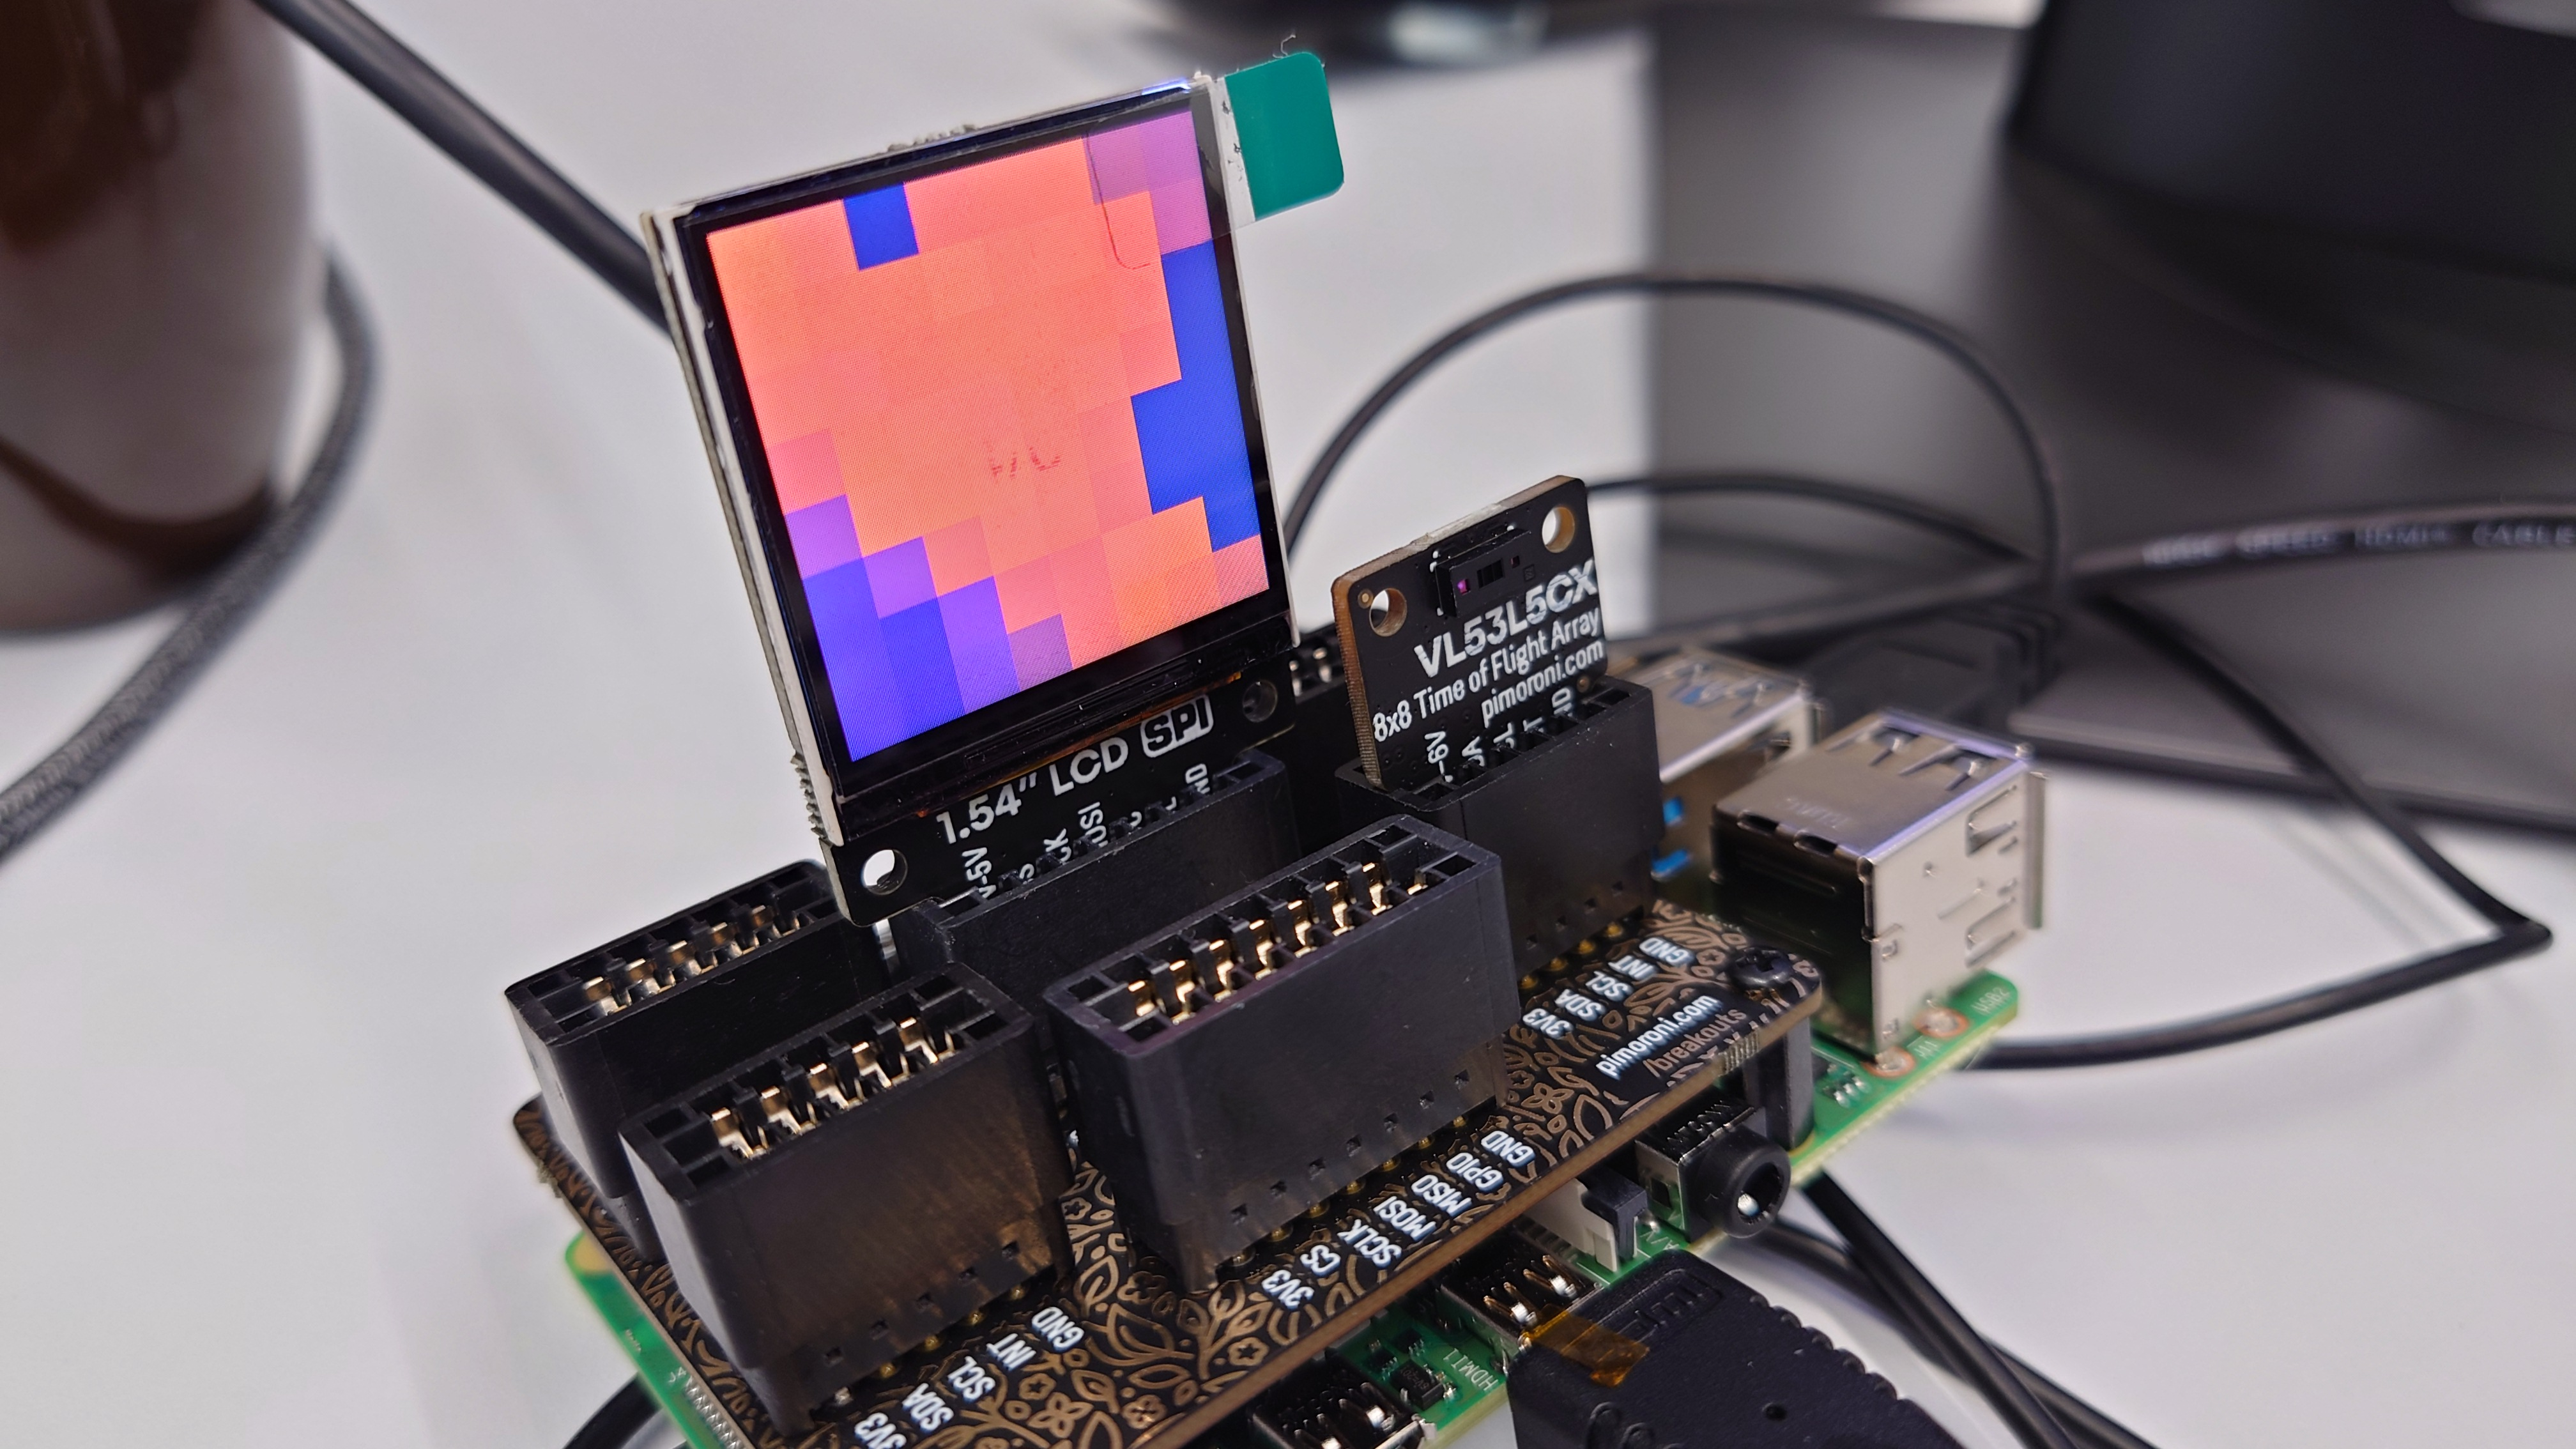
\includegraphics{images/VL53L5CX_LCD.jpg}

}

\caption{\label{fig-vl53l5cx-LCD}Aufbau der Versuchsanordnung für die
Distanzmessung mit dem LCD Bildschirm montiert im dem \emph{hinteren}
SPI Slot}

\end{figure}%

\textbf{Vorbereitung}

\begin{itemize}
\tightlist
\item
  Kontrolliert mit \texttt{python\ -c\ "import\ ST7789"} ob die Library
  \emph{ST7789} installiert ist. Installiere die Library mit
  \texttt{sudo\ pip3\ install\ st7789}, falls sie nicht installiert ist.
  Testet auch, ob die Bibliotheken \texttt{numpy} und
  \texttt{matplotlib} installiert sind und installiert diese ansonsten
  mit \texttt{sudo\ apt\ install\ python3-matplotlib\ python3-numpy}.
\item
  Kontrolliere, ob der Raspberry Pi den \emph{Breakout Garden HAT} mit
  den 2 SPI Anschlüssen und 4 I2C Anschlüssen bestückt ist
  (Abbildung~\ref{fig-vl53l5cx-LCD}).
\item
  Montiere den Bildschirm im hinteren SPI Slot des \emph{Breakout Garden
  HAT}s wie in Abbildung~\ref{fig-vl53l5cx-LCD}, da er sonst die Messung
  des VL53L5CX Sensors verdeckt.
\end{itemize}

Führt nun folgende Scripts aus und beobachtet die Ausgabe auf dem LCD
Bildschirm. Auch hier braucht es etwas Geduld, da die Firmware beim
Starten geladen wird.

\begin{itemize}
\tightlist
\item
  \texttt{python3\ distance\_240x240\_lcd.py}
\item
  \texttt{python3\ motion\_240x240\_lcd.py}
\item
  \texttt{python3\ reflectance\_240x240\_lcd.py}
\item
  \texttt{python3\ motion\_tracking.py}
\end{itemize}

\begin{boxtitle}{Excercise}{colPrimary}

\begin{itemize}
\tightlist
\item
  Führe die Beispiele aus und beobachte die Ausgabe auf dem LCD
  Bildschirm.
\item
  Untersuche die einzelnen Matrizen und versuche die Bedeutung der
  einzelnen Werte zu verstehen.
\item
  Führe unterschiedliche Tests durch, indem Du ein Objekt vor den Sensor
  hälst und bewegst.
\item
  Was passiert wenn Du ein Objekt vor den Sensor hältst? Ist die Form
  erkennbar?
\item
  Was passiert wenn Du ein Objekt vor den Sensor hältst und bewegst?
\item
  Studiere den Code der Beispiele und versuche die Funktionsweise zu
  verstehen.
\item
  Überlege Dir wie Du die Beispiele erweitern könntest.
\end{itemize}

\end{boxtitle}

\chapter*{E05 Thermale Aufnahmen}\label{e05-thermale-aufnahmen}
\addcontentsline{toc}{chapter}{E05 Thermale Aufnahmen}

\markboth{E05 Thermale Aufnahmen}{E05 Thermale Aufnahmen}

Ziel dieser Übung ist es thermale Kamera mit der MLX90640 Kamera kennen
zu lernen und die thermalen Bilddaten auszulesen und testen. Die
\emph{MLX90640} ist eine weitwinkel Kamera mit einer Auflösung von 24x32
Pixel. Sie wird über eine I2C Schnittstelle mit dem Raspberry Pi
verbunden und kann über eine Python Library angesteuert werden.

\textbf{Vorbereitung}

\begin{itemize}
\tightlist
\item
  Schaut folgende von Video von Melexis zur Funktionsweise der MLX90640
  Thermalkamera an:
  \href{https://www.youtube.com/embed/WSZ3GGDusTk?si=WTfxZ3m2axljCwDG}{Far
  Infrared (IR) Thermal Sensor Array 32x24 RES (MLX90640)}
\item
  Studiere das Datenblatt zum VL53L5CX (Melexis 2019) und beantworte
  folgende Fragen:

  \begin{itemize}
  \tightlist
  \item
    In welchen Temperaturbereichen kann der Sensor eingesetzt werden?
  \item
    Welches ist die höchste Abtastrate für die Distanzfeldmessungen?
  \item
    Was sind Anwendungsgebiete für diesen Sensor?
  \end{itemize}
\end{itemize}

\begin{figure}[H]

{\centering 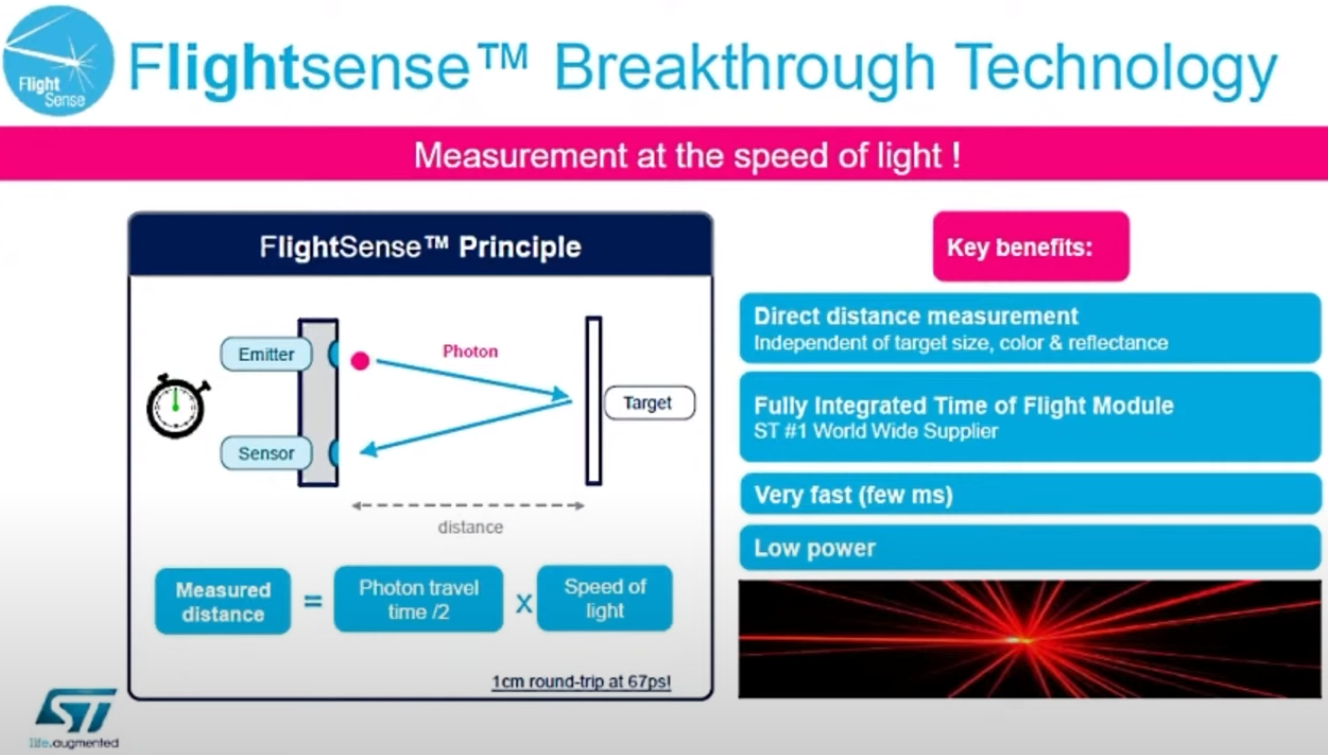
\includegraphics{images/youtube_adafruit_VL53L5CX.png}

}

\caption{Far Infrared (IR) Thermal Sensor Array 32x24 RES (MLX90640)}

\end{figure}%

\begin{longtable}[]{@{}
  >{\raggedright\arraybackslash}p{(\columnwidth - 2\tabcolsep) * \real{0.1429}}
  >{\raggedright\arraybackslash}p{(\columnwidth - 2\tabcolsep) * \real{0.8571}}@{}}
\toprule\noalign{}
\begin{minipage}[b]{\linewidth}\raggedright
\textbf{Unterlagen}
\end{minipage} & \begin{minipage}[b]{\linewidth}\raggedright
\end{minipage} \\
\midrule\noalign{}
\endhead
\bottomrule\noalign{}
\endlastfoot
Produkt &
\href{https://shop.pimoroni.com/products/mlx90640-thermal-camera-breakout?variant=12549161746515}{MLX90640
Breakout} \\
Datenblatt &
\href{https://www.melexis.com/-/media/files/documents/datasheets/mlx90640-datasheet-melexis.pdf}{MLX90640} \\
GitHub &
\href{https://github.com/pimoroni/mlx90640-library}{mlx90640-library},
\href{https://github.com/adafruit/Adafruit_CircuitPython_MLX90640}{Adafruit
MLX90640} \\
\end{longtable}

\section*{\texorpdfstring{MLX90640
Thermalkamera\index{MLX90640}}{MLX90640 Thermalkamera}}\label{mlx90640-thermalkamera}
\addcontentsline{toc}{section}{MLX90640 Thermalkamera\index{MLX90640}}

\markright{MLX90640 Thermalkamera\index{MLX90640}}

Der MLX90640 ist eine Thermalkamera mit einer Auflösung von 32x24 Pixel
mit einem Sichtfeld von 55°. Die Kamera misst in einem Temperaturbereich
von -40° - 300°C mit einer Genauigkeit von etwa 1°C und mit einer
Aufnahmerate von bis zu 64 FPS. Die Anwendungsbereiche sind vielfältig,
von der Temperatur der Kaffeetasse, Hitzeentwicklung in elektronischen
Geräten bis hin zur Überwachung von Gebäuden und Anlagen.

MLX90640 Thermal Camera

\begin{itemize}
\tightlist
\item
  Melexis MLX90640 far-infrared sensor array
\item
  Brennweite: 55°
\item
  32x24 pixels
\item
  I2C interface (address 0x33)
\end{itemize}

\begin{figure}

\centering{

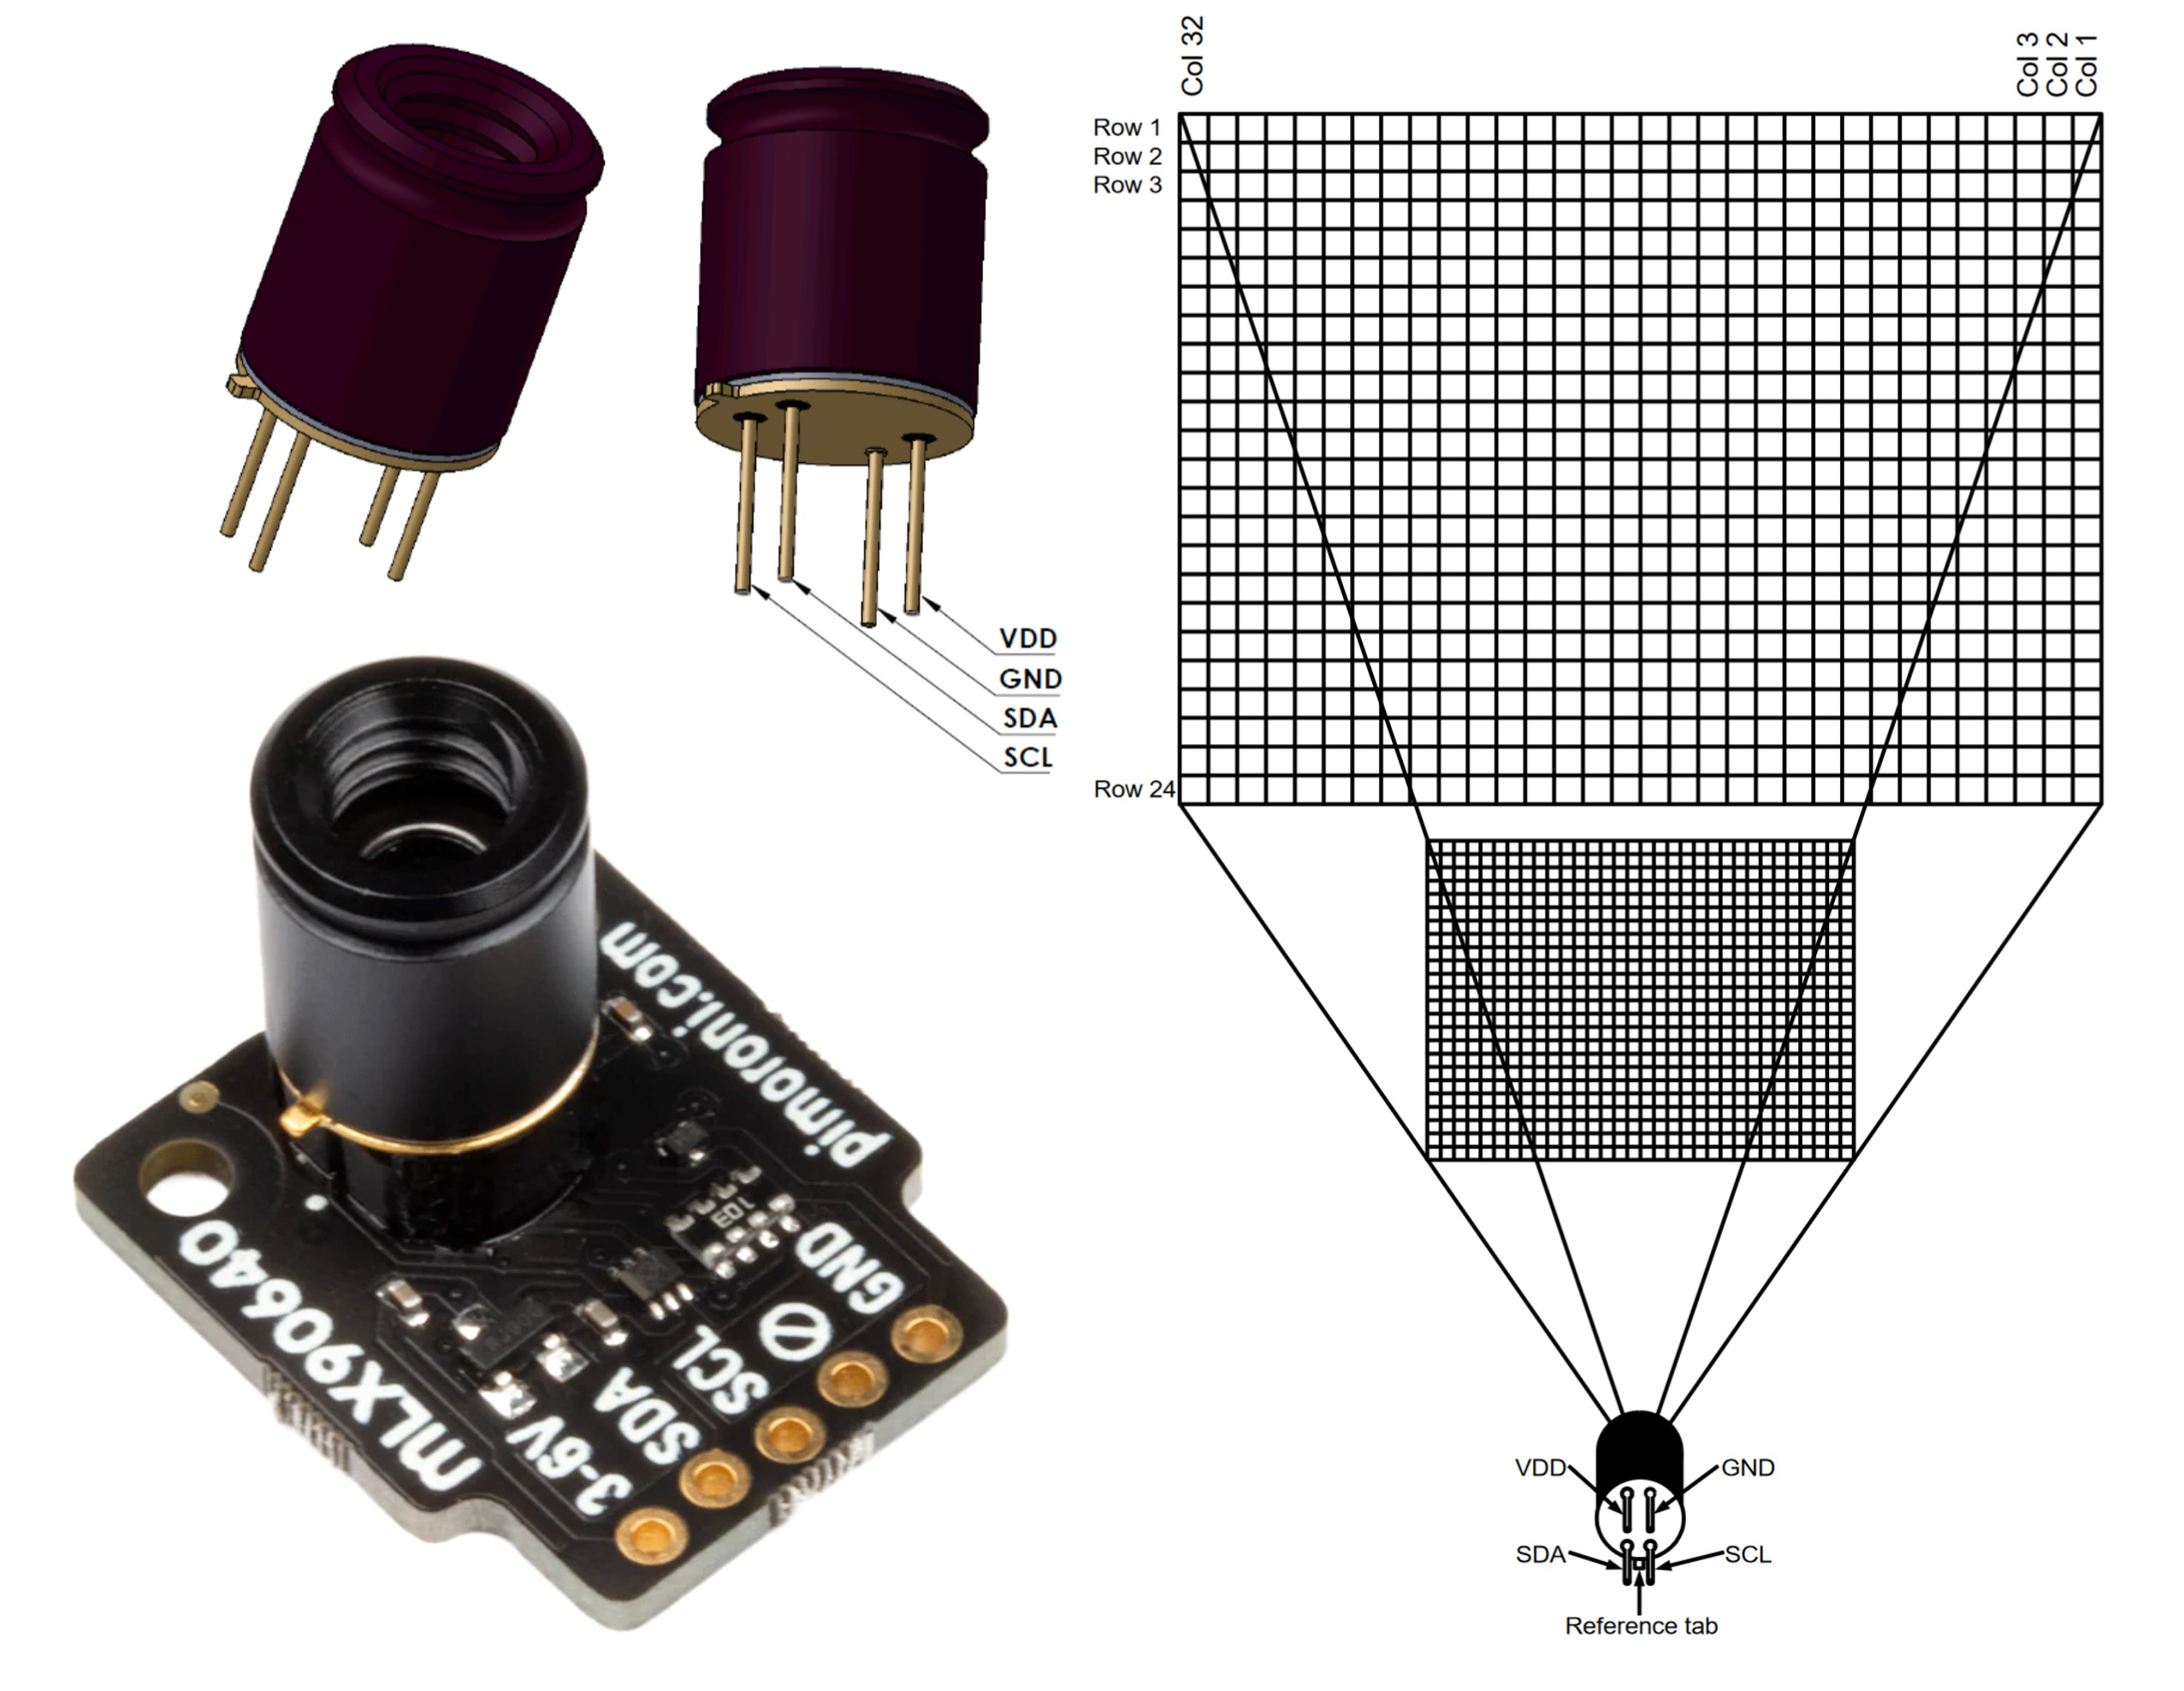
\includegraphics{images/MLX90640_wide.jpg}

}

\caption{\label{fig-MLX90640}links: MLX90640 Thermalkamera, oben:
schematische Darstellung der Kamera und ihrer Anschlüsse rechts:
Pixelpositionaufbau Quelle: STMicroelectronics (2023)}

\end{figure}%

\section*{Übungsaufbau}\label{uxfcbungsaufbau-4}
\addcontentsline{toc}{section}{Übungsaufbau}

\markright{Übungsaufbau}

\begin{itemize}
\tightlist
\item
  Schliesse den Raspberry Pi an Monitor, Keyboard und Maus an oder
  verbinde Dich mit diesem über SSH (und SFTP).
\item
  Erstelle auf dem Raspberry Pi im \texttt{Documents} Ordner einen neuen
  Ordner \texttt{MLX90640}, in welchem Du Änderungen und neue Dateien
  für diese Übung speichern kannst.
\item
  Schliesse den Sensor \textbf{MLX90640} an den Raspberry Pi über die
  Breakout Garden \textbf{I2C} Schnittstelle korrekt an (siehe
  \href{E01_Luftqualitaet.qmd}{E01 Luftqualität}), so dass die
  Beschriftung der Anschlüsse am Sensor und bei der Schnittstelle
  übereinstimmen.
\item
  Kontrolliere mit dem Befehl \texttt{i2cdetect\ -y\ 1} ob der Raspberry
  Pi mit dem Sensor verbunden ist. Der Sensor sollte auf der Adresse
  \texttt{0x33} erkannt werden.
\item
  Kontrolliere, ob folgende Libraries
  \texttt{adafruit-blinka},\texttt{adafruit-circuitpython-mlx90640} und
  \texttt{RPI.GPIO} installiert sind mit
  \texttt{python\ -c\ "import\ adafruit\_mlx90640"}. Installiere die
  Library mit \texttt{sudo\ pip3\ install\ RPI.GPIO\ adafruit-blinka}
  und \texttt{sudo\ pip3\ install\ adafruit-circuitpython-mlx90640}
  falls sie nicht installiert ist.
\end{itemize}

Wechsle in den Ordner \emph{Documents} und kopiere in diesen den Ordner
\emph{MLX90640} mit den Code Beispielen.

\section*{Aufgabe 1: Punktuelle
Temperaturmessung}\label{aufgabe-1-punktuelle-temperaturmessung}
\addcontentsline{toc}{section}{Aufgabe 1: Punktuelle Temperaturmessung}

\markright{Aufgabe 1: Punktuelle Temperaturmessung}

Teste das Beispiel \texttt{thermal\_camera\_average\_temperature.py} im
Ordner \emph{examples}. Dieses Beispiel liest die Werte aus der Matrix
der Thermalkamera und gibt den Mittelwert der Temperatur aus. Die
Ausgabe sollte in etwa so aussehen (gekürzt):

\begin{Shaded}
\begin{Highlighting}[]
\ExtensionTok{python3}\NormalTok{ average\_temperature.py }
\ExtensionTok{Average}\NormalTok{ MLX90640 Temperature: 23.6C }\ErrorTok{(}\ExtensionTok{74.5F}\KeywordTok{)}
\end{Highlighting}
\end{Shaded}

Folgendes Code Snippet zeigt eine gekürzte Version des
\texttt{thermal\_camera\_average\_temperature.py} Python Beispiels für
die Ausgabe der Distanzmatrix.

\phantomsection\label{annotated-cell-23}%
\begin{Shaded}
\begin{Highlighting}[]
\ImportTok{import}\NormalTok{ time,board,busio}
\ImportTok{import}\NormalTok{ numpy }\ImportTok{as}\NormalTok{ np}
\ImportTok{import}\NormalTok{ adafruit\_mlx90640}

\NormalTok{i2c }\OperatorTok{=}\NormalTok{ busio.I2C(board.SCL, board.SDA) }\hspace*{\fill}\NormalTok{\circled{1}}
\NormalTok{mlx }\OperatorTok{=}\NormalTok{ adafruit\_mlx90640.MLX90640(i2c) }
\NormalTok{mlx.refresh\_rate }\OperatorTok{=}\NormalTok{ adafruit\_mlx90640.RefreshRate.REFRESH\_2\_HZ }

\NormalTok{frame }\OperatorTok{=}\NormalTok{ np.zeros((}\DecValTok{24}\OperatorTok{*}\DecValTok{32}\NormalTok{,)) }\hspace*{\fill}\NormalTok{\circled{2}}
\ControlFlowTok{while} \VariableTok{True}\NormalTok{:}
    \ControlFlowTok{try}\NormalTok{:}
\NormalTok{        mlx.getFrame(frame) }\hspace*{\fill}\NormalTok{\circled{3}}
        \ControlFlowTok{break}
    \ControlFlowTok{except} \PreprocessorTok{ValueError}\NormalTok{:}
        \ControlFlowTok{continue} \hspace*{\fill}\NormalTok{\circled{4}}

\CommentTok{\# print out the average temperature from the MLX90640}
\BuiltInTok{print}\NormalTok{(}\StringTok{\textquotesingle{}Average MLX90640 Temperature: }\SpecialCharTok{\{0:2.1f\}}\StringTok{C (}\SpecialCharTok{\{1:2.1f\}}\StringTok{F)\textquotesingle{}}\NormalTok{.\textbackslash{} }\hspace*{\fill}\NormalTok{\circled{5}}
      \BuiltInTok{format}\NormalTok{(np.mean(frame),(((}\FloatTok{9.0}\OperatorTok{/}\FloatTok{5.0}\NormalTok{)}\OperatorTok{*}\NormalTok{np.mean(frame))}\OperatorTok{+}\FloatTok{32.0}\NormalTok{))) }
\end{Highlighting}
\end{Shaded}

\begin{description}
\tightlist
\item[\circled{1}]
Setup von I2C, Initialisierung des MLX90640 Sensors und Setzen der
Abtastrate auf 2 Hz
\item[\circled{2}]
Numpy Array für das Speichern der 768 Temperaturwerte (24x32 Pixel)
erstellen
\item[\circled{3}]
MLX Temperaturwerte in das Numpy Array speichern
\item[\circled{4}]
Falls ein Fehler eintritt, nochmals versuchen den Sensor auszulesen
\item[\circled{5}]
Temperaturmittelwert ausgeben
\end{description}

\begin{boxtitle}{Excercise}{colPrimary}

\textbf{Einzelne Temperaturmessung}

\begin{itemize}
\tightlist
\item
  Führe das Beispiel \texttt{average\_temperature.py} aus und beobachte
  die Messwerte.
\item
  Teste das Script mit unterschiedlichen warmen Objekten (z.B.
  Kaffeetasse, Hand, etc.).
\end{itemize}

\end{boxtitle}

\section*{Aufgabe 2: Thermale Aufnahme mit LCD
Bildschirm}\label{aufgabe-2-thermale-aufnahme-mit-lcd-bildschirm}
\addcontentsline{toc}{section}{Aufgabe 2: Thermale Aufnahme mit LCD
Bildschirm}

\markright{Aufgabe 2: Thermale Aufnahme mit LCD Bildschirm}

Folgende Aufgabe nutzt den 1.54'' LCD Bildschirm mit einer 240x240 Pixel
Auflösung. Der Ordner enthält mehrere Beispiele zur Thermalkamera, die
die Temperaturmatrix auf dem Bildschirm anzeigen. Die Beispiele sind im
Ordner \texttt{MLX90640} zu finden.

\begin{figure}

\centering{

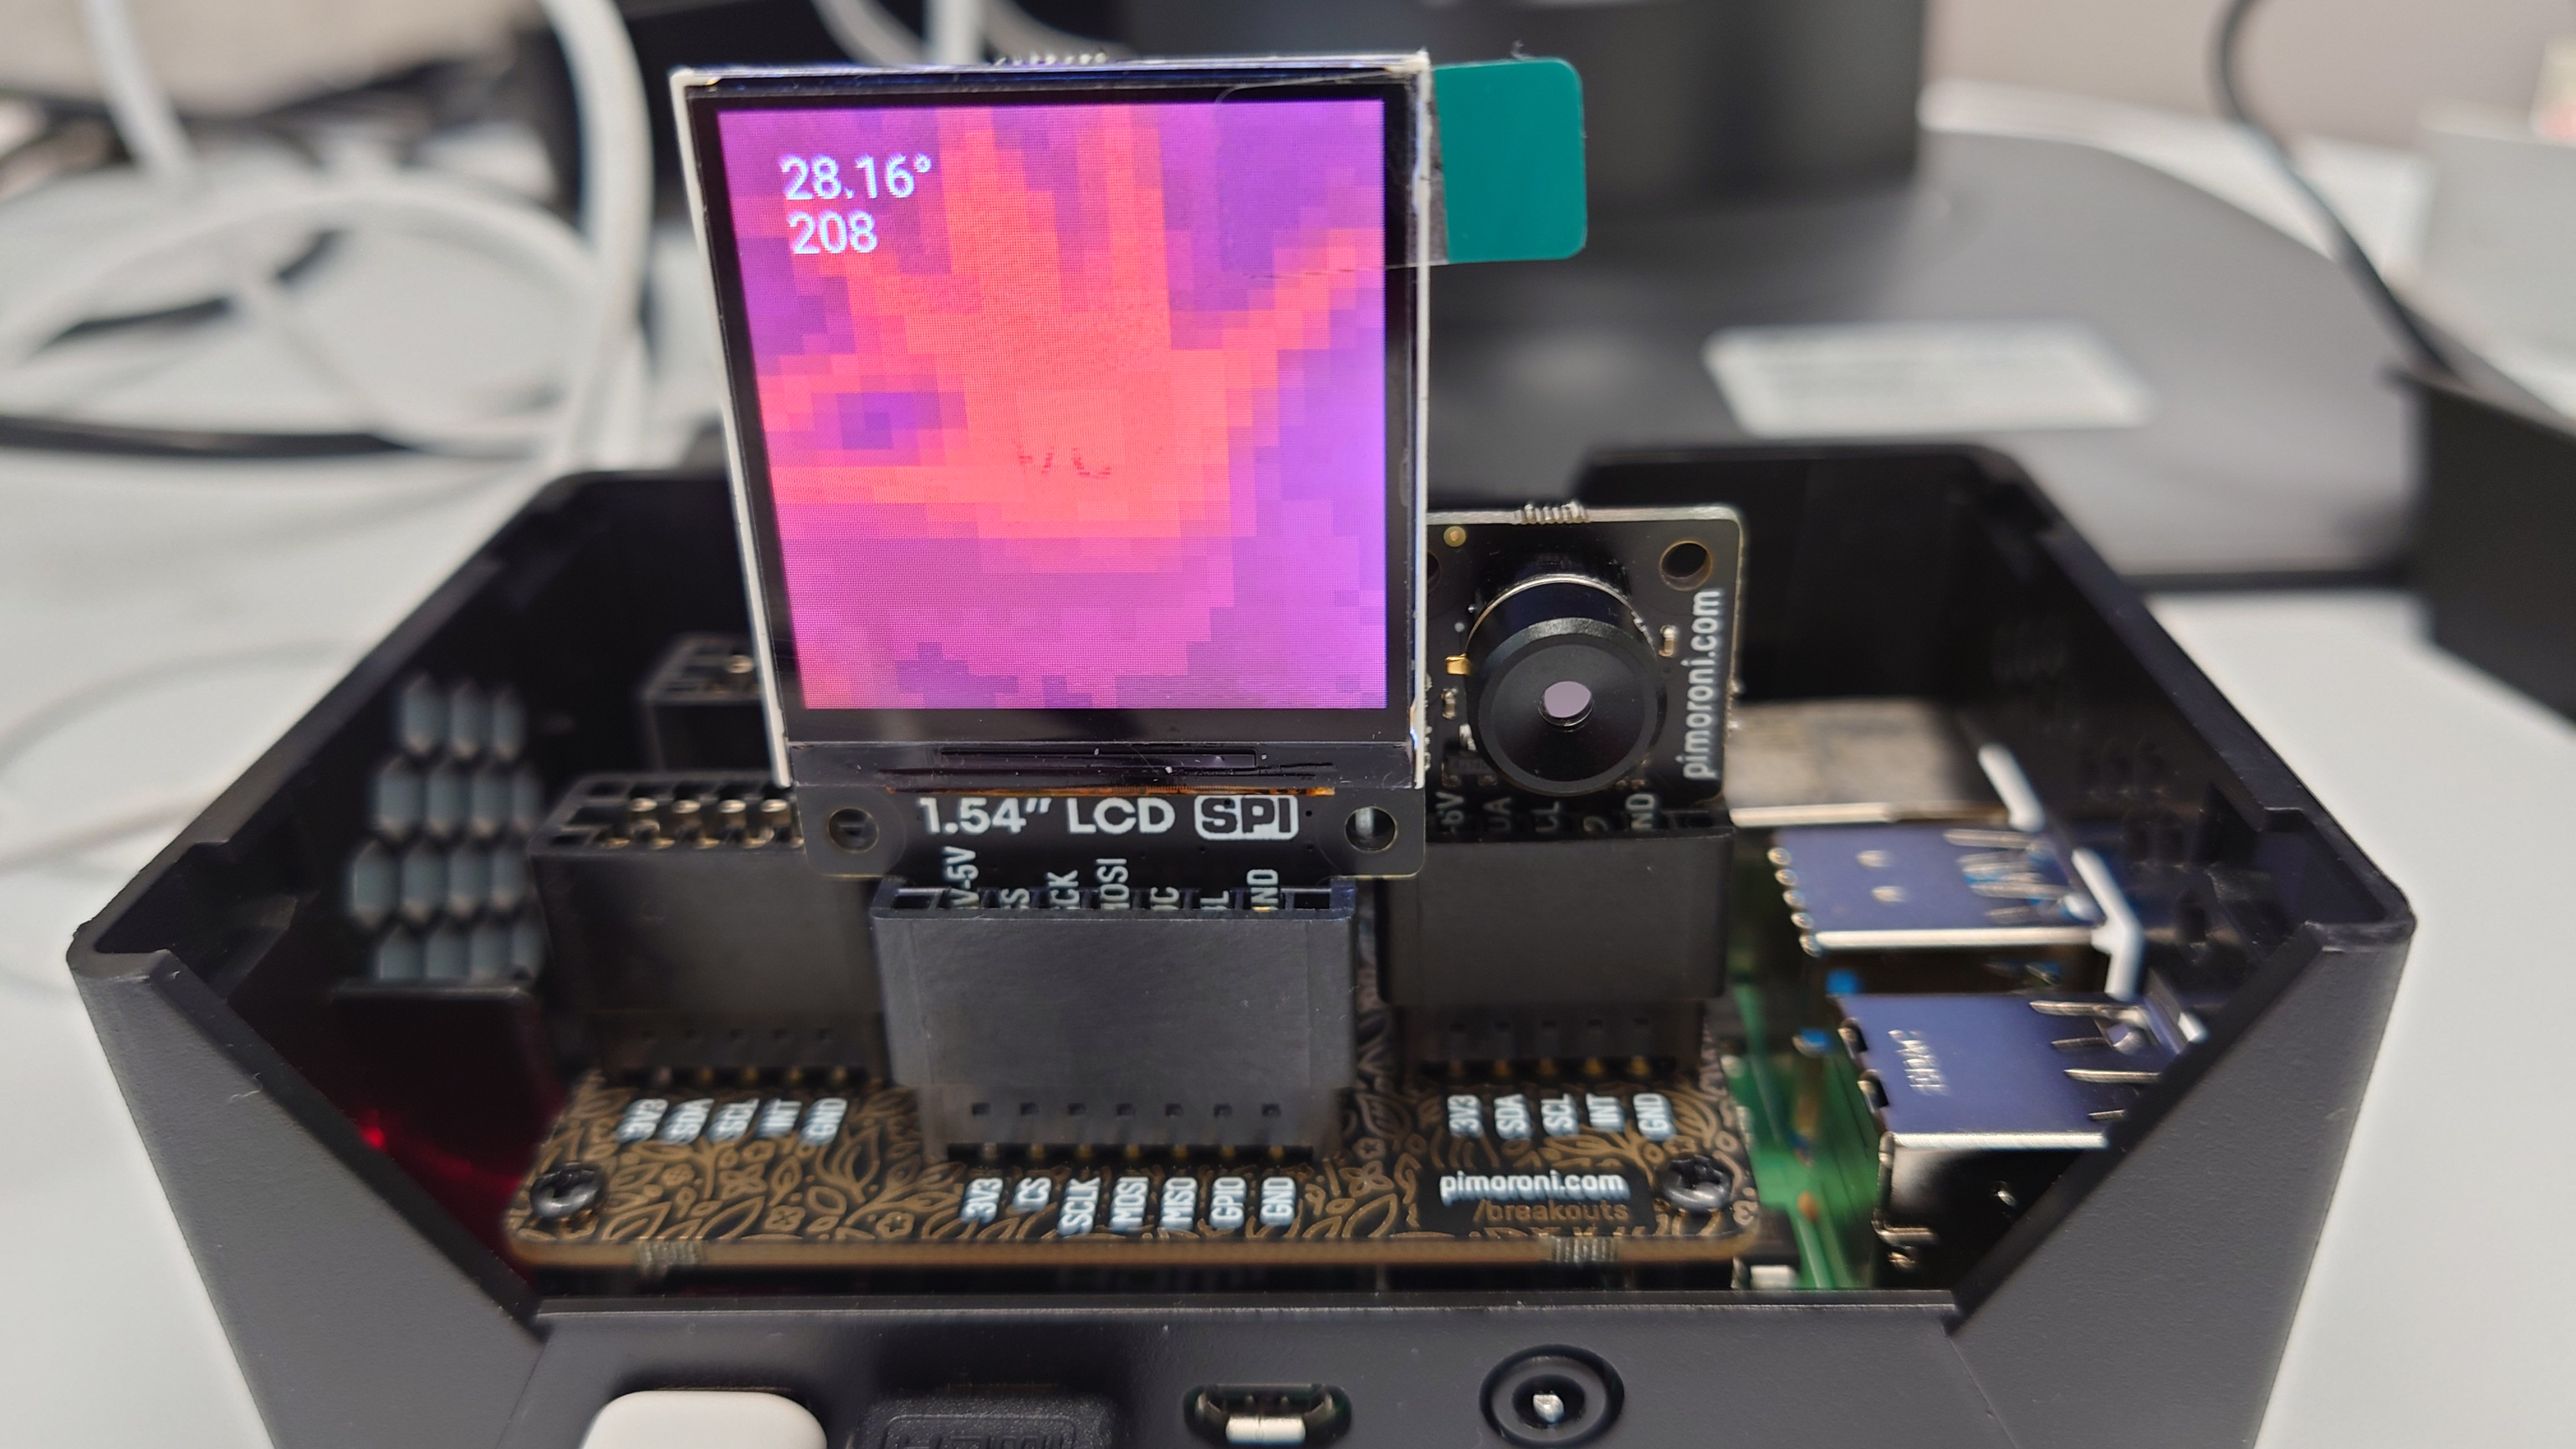
\includegraphics{images/MLX90640_LCD.jpg}

}

\caption{\label{fig-mlx90640-LCD}Aufbau der Versuchsanordnung für die
Distanzmessung mit dem LCD Bildschirm montiert im dem \emph{hinteren}
SPI Slot}

\end{figure}%

\textbf{Vorbereitung}

\begin{itemize}
\tightlist
\item
  Kontrolliert mit \texttt{python\ -c\ "import\ ST7789"} ob die Library
  \emph{ST7789} installiert ist. Installiere die Library mit
  \texttt{sudo\ pip3\ install\ st7789}, falls sie nicht installiert ist.
  Testet auch, ob die Bibliotheken \texttt{numpy} und
  \texttt{matplotlib} installiert sind und installiert diese ansonsten
  mit \texttt{sudo\ apt\ install\ python3-matplotlib\ python3-numpy}.
\item
  Kontrolliere, ob der Raspberry Pi den \emph{Breakout Garden HAT} mit
  den 2 SPI Anschlüssen und 4 I2C Anschlüssen bestückt ist
  (Abbildung~\ref{fig-mlx90640-LCD}).
\item
  Montiere den Bildschirm im vorderen SPI Slot des \emph{Breakout Garden
  HAT}s wie in Abbildung~\ref{fig-mlx90640-LCD}, oder passe das Script,
  an so dass die Werte der hinteren SPI Schnittstelle verwendet werden.
\item
  Teste die Beispiele im Ordner \texttt{MLX90640} und beobachte die
  Ausgabe auf dem LCD Bildschirm.
\end{itemize}

\begin{boxtitle}{Excercise}{colPrimary}

\begin{itemize}
\tightlist
\item
  Teste mit unterschiedlichen Objekten die Temperaturmessung und
  beobachte die Ausgabe auf dem LCD Bildschirm.
\item
  Wie gut lassen sich Objekte mit unterschiedlichen Temperaturen
  unterscheiden?
\item
  Wie gut lassen sich Objekte erkennen, die sich in der Temperatur nur
  wenig oder stark unterscheiden?
\item
  Studiere den Code der Beispiele und versuche die Funktionsweise zu
  verstehen.
\item
  Überlege Dir, wie Du die Beispiele erweitern könntest.
\end{itemize}

\end{boxtitle}

\chapter*{E06 Biometrie}\label{e06-biometrie}
\addcontentsline{toc}{chapter}{E06 Biometrie}

\markboth{E06 Biometrie}{E06 Biometrie}

Ziel dieser Übung ist es biometrische Messungen mit dem \emph{MAX30101}
Sensor durchzuführen und den Sensor in seiner funktionsweise zu
untersuchen. Der \emph{MAX30101} ist ein Sensor zur Messung der
Herzfrequenz und der Sauerstoffsättigung im Blut und ein
Rauch-/Partikelsensor. Er verfügt über eine I2C Schnittstelle und kann
über eine Python Library angesteuert werden.

\textbf{Vorbereitung}

\begin{itemize}
\tightlist
\item
  Schaut Euch folgendes von Video von Peter Charlton zur Funktionsweise
  der Herzfrequenzmessung an:
  \href{https://www.youtube.com/embed/HnXDvN4WNX8?si=EeIAlSWW2Z1SJBof}{Photoplethysmography
  in a minute (and a bit) - Peter Charlton}
\item
  Studiere das Datenblatt zum MAX30101 (maxim integrated 2020)

  \begin{itemize}
  \tightlist
  \item
    In welchen Temperaturbereichen kann der Sensor eingesetzt werden?
  \item
    Welches ist die höchste Abtastrate für die Sauerstoffmessungen?
  \item
    Was sind Anwendungsgebiete für diesen Sensor?
  \end{itemize}
\end{itemize}

\begin{figure}[H]

{\centering 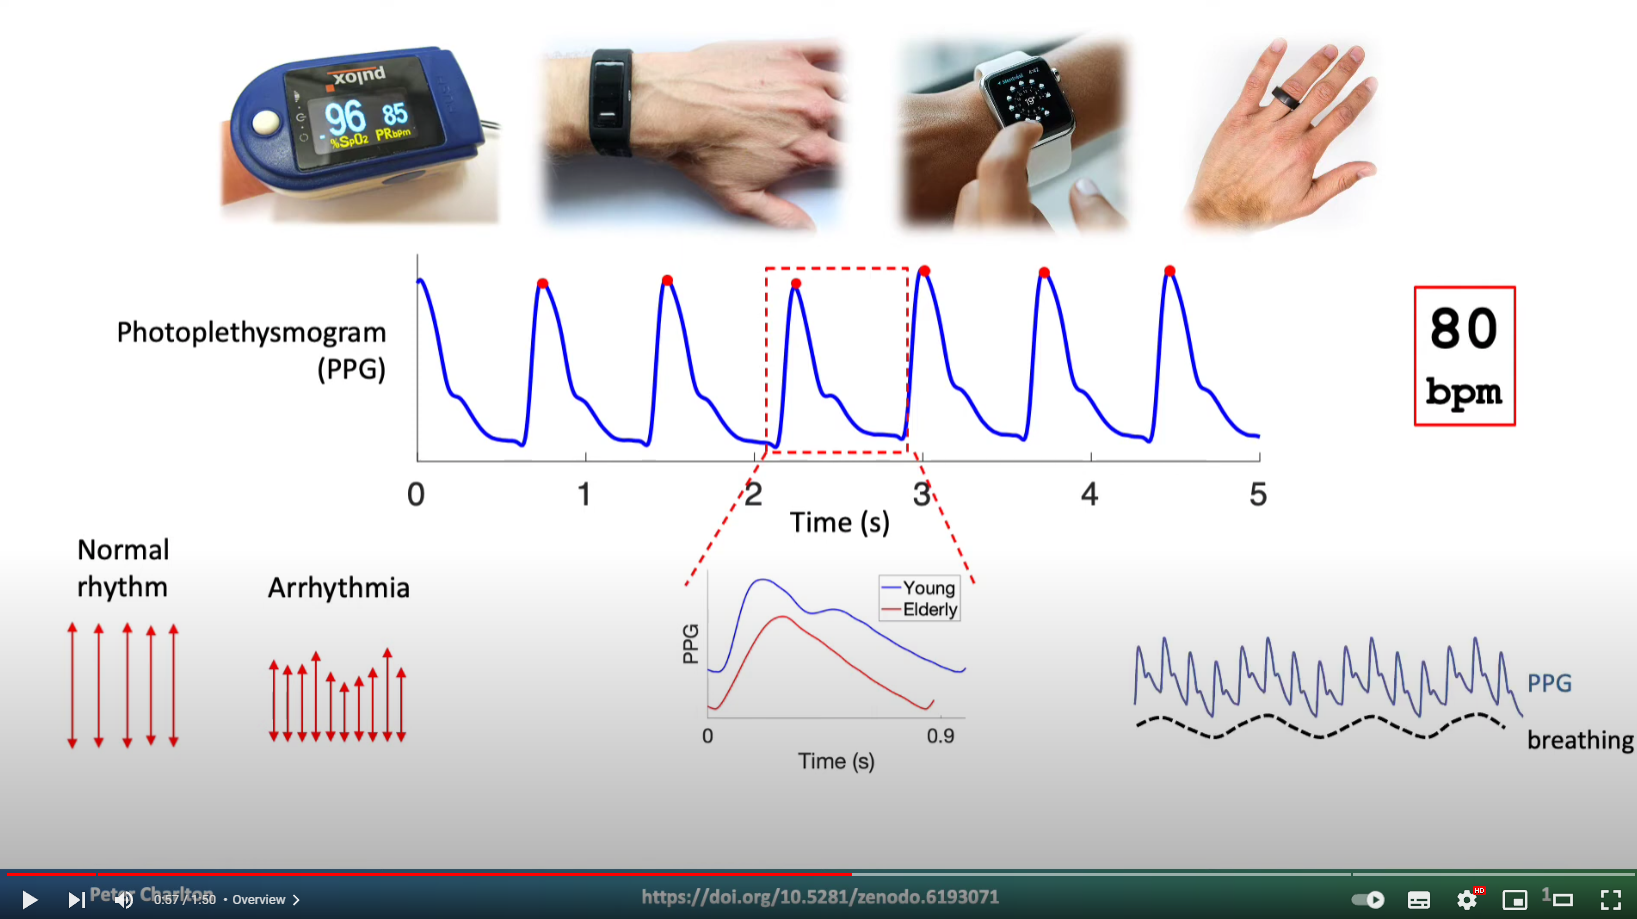
\includegraphics{images/youtube_photoplethysmography.png}

}

\caption{Photoplethysmography in a minute (and a bit) - Peter Charlton}

\end{figure}%

\begin{longtable}[]{@{}
  >{\raggedright\arraybackslash}p{(\columnwidth - 2\tabcolsep) * \real{0.1429}}
  >{\raggedright\arraybackslash}p{(\columnwidth - 2\tabcolsep) * \real{0.8571}}@{}}
\toprule\noalign{}
\begin{minipage}[b]{\linewidth}\raggedright
\textbf{Unterlagen}
\end{minipage} & \begin{minipage}[b]{\linewidth}\raggedright
\end{minipage} \\
\midrule\noalign{}
\endhead
\bottomrule\noalign{}
\endlastfoot
Produkt &
\href{https://shop.pimoroni.com/products/max30101-breakout-heart-rate-oximeter-smoke-sensor}{MAX30101
Breakout} \\
Datenblatt &
\href{https://datasheets.maximintegrated.com/en/ds/MAX30101.pdf}{MAX30101} \\
GitHub &
\href{https://github.com/pimoroni/max30105-python}{max30105-python} \\
\end{longtable}

\section*{\texorpdfstring{MAX30101 Breakout Heart Rate, Oximeter, Smoke
Sensor\index{MAX30101}}{MAX30101 Breakout Heart Rate, Oximeter, Smoke Sensor}}\label{max30101-breakout-heart-rate-oximeter-smoke-sensor}
\addcontentsline{toc}{section}{MAX30101 Breakout Heart Rate, Oximeter,
Smoke Sensor\index{MAX30101}}

\markright{MAX30101 Breakout Heart Rate, Oximeter, Smoke
Sensor\index{MAX30101}}

Der MAX30101 ist hochentwickelter Herzfrequenz-, Oximeter- und
Rauch-/Partikelsensor. Der Sensor verfügt über drei LEDs (rot, grün, IR)
und Photodetektoren. Mit der Photoplethysmographie (photoplethysmography
PPG) kann über die Farbveränderung der Haut bei jedem Herzschlag dieser
detektiert werden, wenn der Sensor leicht auf den Finger gedrückt wird.
Der Sensor kann auch dazu benutzt werden um Partikel in der Luft wie
rauch zu erkennen, in dem er die Lichtmenge, die von Partikeln in der
Luft zurückgeworfen wird misst.

MAX30101 Breakout - Heart Rate, Oximeter, Smoke Sensor Breakout

\begin{itemize}
\tightlist
\item
  MAX30101 - heart rate, oximeter, smoke sensor
\item
  Green, red, and infra-red LEDs
\item
  Photodetectors
\item
  Ambient light rejection
\item
  Temperature sensor
\end{itemize}

\begin{figure}

\centering{

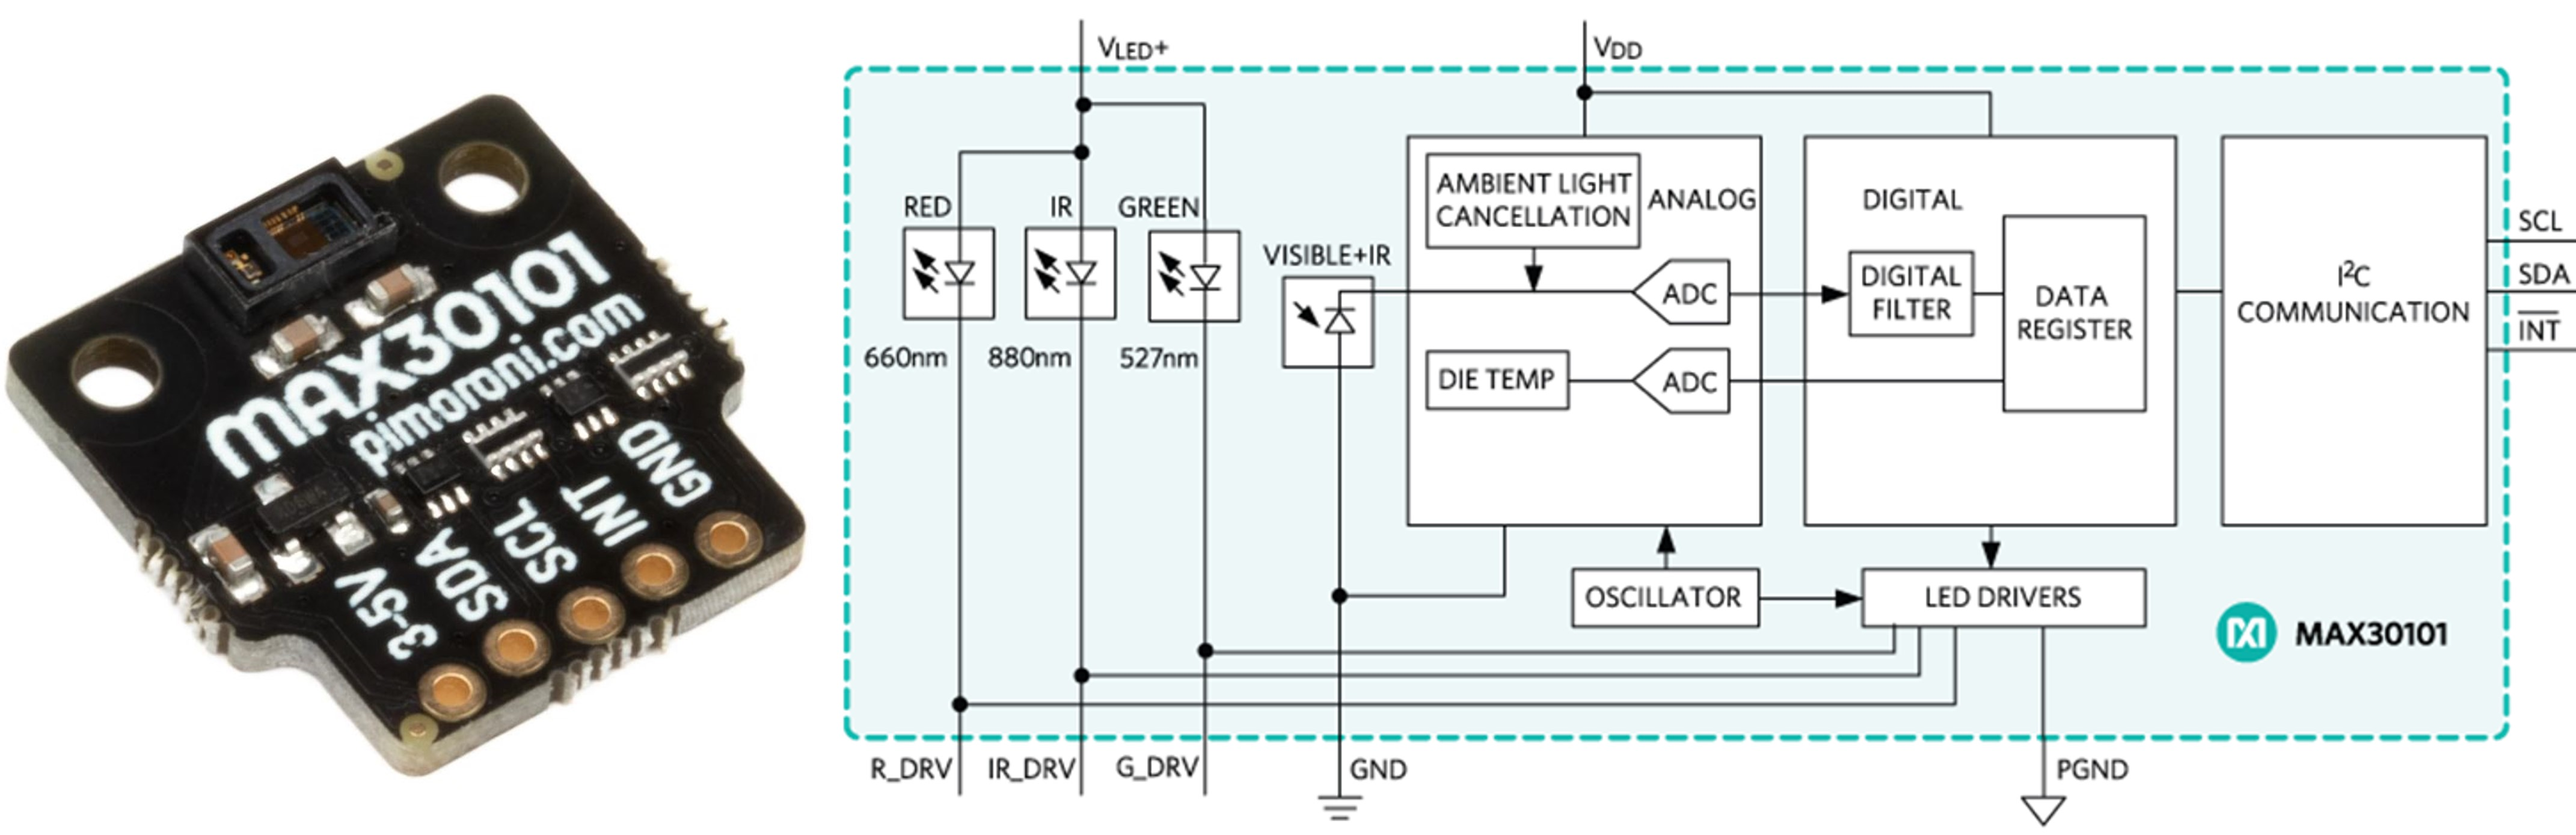
\includegraphics{images/MAX30101_wide.jpg}

}

\caption{\label{fig-MAX30101}links: MAX30101 Breakout von Pimoroni,
rechts: funktionale Diagram des MAX30101 Moduls Quelle: maxim integrated
(2020)}

\end{figure}%

\section*{Übungsaufbau}\label{uxfcbungsaufbau-5}
\addcontentsline{toc}{section}{Übungsaufbau}

\markright{Übungsaufbau}

\begin{itemize}
\tightlist
\item
  Schliesse den Raspberry Pi an Monitor, Keyboard und Maus an oder
  verbinde Dich mit diesem über SSH (und SFTP).
\item
  Erstelle auf dem Raspberry Pi im \texttt{Documents} Ordner einen neuen
  Ordner \texttt{MAX30101}, in welchem Du Änderungen und neue Dateien
  für diese Übung speichern kannst.
\item
  Schliesse den Sensor \textbf{MAX30101} an den Raspberry Pi über die
  Breakout Garden \textbf{I2C} Schnittstelle korrekt an (siehe
  \href{E01_Luftqualitaet.qmd}{E01 Luftqualität}), so dass die
  Beschriftung der Anschlüsse am Sensor und bei der Schnittstelle
  übereinstimmen.
\item
  Kontrolliere mit dem Befehl \texttt{i2cdetect\ -y\ 1} ob der Raspberry
  Pi mit dem Sensor verbunden ist. Der Sensor sollte auf der Adresse
  \texttt{0x29} erkannt werden.
\item
  Kontrolliere, ob die Library \texttt{vl53l5cx\_ctypes} installiert ist
  mit \texttt{python\ -c\ "import\ vl53l5cx\_ctypes"}. Installiere die
  Library mit \texttt{sudo\ pip3\ install\ vl53l5cx-ctypes} falls sie
  nicht installiert ist.
\end{itemize}

Wechsle in den Ordner \emph{Documents} und kopiere mit folgenden
Befehlen die Library auf Deinen Raspberry Pi.

\begin{Shaded}
\begin{Highlighting}[]
\BuiltInTok{cd}\NormalTok{ Documents}
\FunctionTok{git}\NormalTok{ clone https://github.com/pimoroni/max30105{-}python}
\BuiltInTok{cd}\NormalTok{ max30105{-}python/examples}
\end{Highlighting}
\end{Shaded}

\section*{Aufgabe 1: Distanzmessung
Konsole}\label{aufgabe-1-distanzmessung-konsole-1}
\addcontentsline{toc}{section}{Aufgabe 1: Distanzmessung Konsole}

\markright{Aufgabe 1: Distanzmessung Konsole}

Teste das Beispiel \texttt{read-heartbeat.py} im Ordner \emph{examples}.
Dieses Beispiel liest die Pulsschläge pro Minute in PPM (beats per
minute). Ein erkannter Pulsschlag wird mit einem \texttt{\textless{}3}
angezeigt.

Startet das Script mit \texttt{python3\ read-heartbeat.py}. Mit
\texttt{Ctrl+c} kann das Script wieder gestopppt wrden. Die Ausgabe
sollte in etwa so aussehen (gekürzt):

\begin{Shaded}
\begin{Highlighting}[]
\ExtensionTok{python3}\NormalTok{ read{-}heartbeat.py }
\ExtensionTok{NOTE!}\NormalTok{ This code should not be used for medical diagnosis. }
\ExtensionTok{...}
\ExtensionTok{Starting}\NormalTok{ readings in 10 seconds...}

   \ExtensionTok{BPM:}\NormalTok{ 0.00  AVG: 0.00}
   \ExtensionTok{BPM:}\NormalTok{ 0.00  AVG: 0.00}
   \ExtensionTok{BPM:}\NormalTok{ 0.00  AVG: 0.00}
   \ExtensionTok{BPM:}\NormalTok{ 0.00  AVG: 0.00}
   \ExtensionTok{BPM:}\NormalTok{ 45.55  AVG: 45.96}
\OperatorTok{\textless{}}\NormalTok{3 }\ExtensionTok{BPM:}\NormalTok{ 55.75  AVG: 59.90}
   \ExtensionTok{BPM:}\NormalTok{ 55.75  AVG: 59.90}
\OperatorTok{\textless{}}\NormalTok{3 }\ExtensionTok{BPM:}\NormalTok{ 59.64  AVG: 70.65}
   \ExtensionTok{BPM:}\NormalTok{ 59.64  AVG: 70.65}
\end{Highlighting}
\end{Shaded}

Folgendes Code Snippet zeigt eine gekürtzte Version des
\texttt{read-heartbeat.py} Python Beispiels für die Ausgabe des
Herzschlags.

\phantomsection\label{annotated-cell-26}%
\begin{Shaded}
\begin{Highlighting}[]
\CommentTok{\#!/usr/bin/env python}

\CommentTok{\# }\AlertTok{NOTE}\CommentTok{! This code should not be used for medical diagnosis. It\textquotesingle{}s}
\CommentTok{\# for fun/novelty use only, so bear that in mind while using it.}

\ImportTok{import}\NormalTok{ time}
\ImportTok{from}\NormalTok{ max30105 }\ImportTok{import}\NormalTok{ MAX30105, HeartRate}

\NormalTok{max30105 }\OperatorTok{=}\NormalTok{ MAX30105() }\hspace*{\fill}\NormalTok{\circled{1}}
\NormalTok{max30105.setup(leds\_enable}\OperatorTok{=}\DecValTok{2}\NormalTok{) }\hspace*{\fill}\NormalTok{\circled{2}}
\NormalTok{max30105.set\_led\_pulse\_amplitude(}\DecValTok{1}\NormalTok{, }\FloatTok{0.2}\NormalTok{) }
\NormalTok{max30105.set\_led\_pulse\_amplitude(}\DecValTok{2}\NormalTok{, }\FloatTok{12.5}\NormalTok{) }
\NormalTok{max30105.set\_led\_pulse\_amplitude(}\DecValTok{3}\NormalTok{, }\DecValTok{0}\NormalTok{) }
\NormalTok{max30105.set\_slot\_mode(}\DecValTok{1}\NormalTok{, }\StringTok{\textquotesingle{}red\textquotesingle{}}\NormalTok{) }
\NormalTok{max30105.set\_slot\_mode(}\DecValTok{2}\NormalTok{, }\StringTok{\textquotesingle{}ir\textquotesingle{}}\NormalTok{) }
\NormalTok{max30105.set\_slot\_mode(}\DecValTok{3}\NormalTok{, }\StringTok{\textquotesingle{}off\textquotesingle{}}\NormalTok{) }
\NormalTok{max30105.set\_slot\_mode(}\DecValTok{4}\NormalTok{, }\StringTok{\textquotesingle{}off\textquotesingle{}}\NormalTok{) }

\KeywordTok{def}\NormalTok{ display\_heartrate(beat, bpm, avg\_bpm): }\hspace*{\fill}\NormalTok{\circled{3}}
    \BuiltInTok{print}\NormalTok{(}\StringTok{"}\SpecialCharTok{\{\}}\StringTok{ BPM: }\SpecialCharTok{\{:.2f\}}\StringTok{  AVG: }\SpecialCharTok{\{:.2f\}}\StringTok{"}\NormalTok{.}\BuiltInTok{format}\NormalTok{(}\StringTok{"\textless{}3"} \ControlFlowTok{if}\NormalTok{ beat }\ControlFlowTok{else} \StringTok{"  "}\NormalTok{,}
\NormalTok{          bpm, avg\_bpm))}
\NormalTok{hr }\OperatorTok{=}\NormalTok{ HeartRate(max30105) }\hspace*{\fill}\NormalTok{\circled{4}}

\NormalTok{delay }\OperatorTok{=} \DecValTok{10} \hspace*{\fill}\NormalTok{\circled{5}}
\BuiltInTok{print}\NormalTok{(}\StringTok{"Starting readings in }\SpecialCharTok{\{\}}\StringTok{ seconds...}\CharTok{\textbackslash{}n}\StringTok{"}\NormalTok{.}\BuiltInTok{format}\NormalTok{(delay)) }
\NormalTok{time.sleep(delay) }

\ControlFlowTok{try}\NormalTok{:}
\NormalTok{    hr.on\_beat(display\_heartrate, average\_over}\OperatorTok{=}\DecValTok{4}\NormalTok{) }\hspace*{\fill}\NormalTok{\circled{6}}
\ControlFlowTok{except} \PreprocessorTok{KeyboardInterrupt}\NormalTok{:}
    \ControlFlowTok{pass}
\end{Highlighting}
\end{Shaded}

\begin{description}
\tightlist
\item[\circled{1}]
Sensor initialisieren
\item[\circled{2}]
Sensor konfigurieren (LED Pulse Amplitude, Slot Mode der LED)
\item[\circled{3}]
Funktion zur Darstellung des Herzschlags in der Konsole
\item[\circled{4}]
Initialisierung des Herzschlagdetektors
\item[\circled{5}]
10 Sekeunden warten und dann die Herzschläge ausgeben
\item[\circled{6}]
Bei einem erkannten Herzschlag wird die Funktion
\texttt{display\_heartrate} aufgerufen und der Herzschlag wird über 4
Sekunden gemittelt in der Konsole ausgegeben.
\end{description}

\begin{boxtitle}{Excercise}{colPrimary}

\textbf{Pulsmessung}

\begin{itemize}
\tightlist
\item
  Führe das Beispiel \texttt{read-heartbeat.py} aus und beobachte die
  Messwerte.
\item
  Führe unterschiedliche Tests durch und behandle den Sensor freundlich.
\item
  Vergleiche die Messwerte und kontrolliere die Werte in dem Du den
  eigenen Puls misst oder mit einem Sportuhr vergleichst.
\item
  Studiere den Code der Beispiele und versuche die Funktionsweise zu
  verstehen.
\end{itemize}

\end{boxtitle}

\chapter*{E07 MQTT}\label{e07-mqtt}
\addcontentsline{toc}{chapter}{E07 MQTT}

\markboth{E07 MQTT}{E07 MQTT}

Ein IoT Datenfluss erstreckt sich über verschiedene Instanzen, die für
die einzelnen Prozesse zuständig sind, von der Erfassung von
Sensormesswerten im IoT Gerät über die Kommunikation der Messwerte bis
zur Datenverarbeitung, Speicherung und Visualisierung
(Abbildung~\ref{fig-iotpipeline}). Hierbei können alle Schritte auf
einem Gerät durchgeführt werden oder jeder einzelne über ein anderes
Gerät oder Server. In der Abbildung aufgezeigt sind typische
Softwarekomponenten, die in IoT eingesetzt werden, wie Node-Red für die
Datenverarbeitung, die InfluxDB Datenbank, welche für das Speichern von
Zeitreihendaten entwickelt wurde und Grafana eine
Visualisierungsplattform, die für Messdaten optimiert ist. Es sind
Werkzeuge die über ihre graphische Oberfläche einen guten Einstieg
ermöglichen, sogenannte \emph{low-code} Tools, die sich gut eignen für
die Entwicklung von Prototypen mit geringem zeitlichen Aufwand. Je nach
Anwendung können die einzelnen Prozessschritte auch gut in einer
Scriptsprache wie Python durchgeführt oder eine andere Datenbank
verwendet werden.

\begin{figure}

\centering{

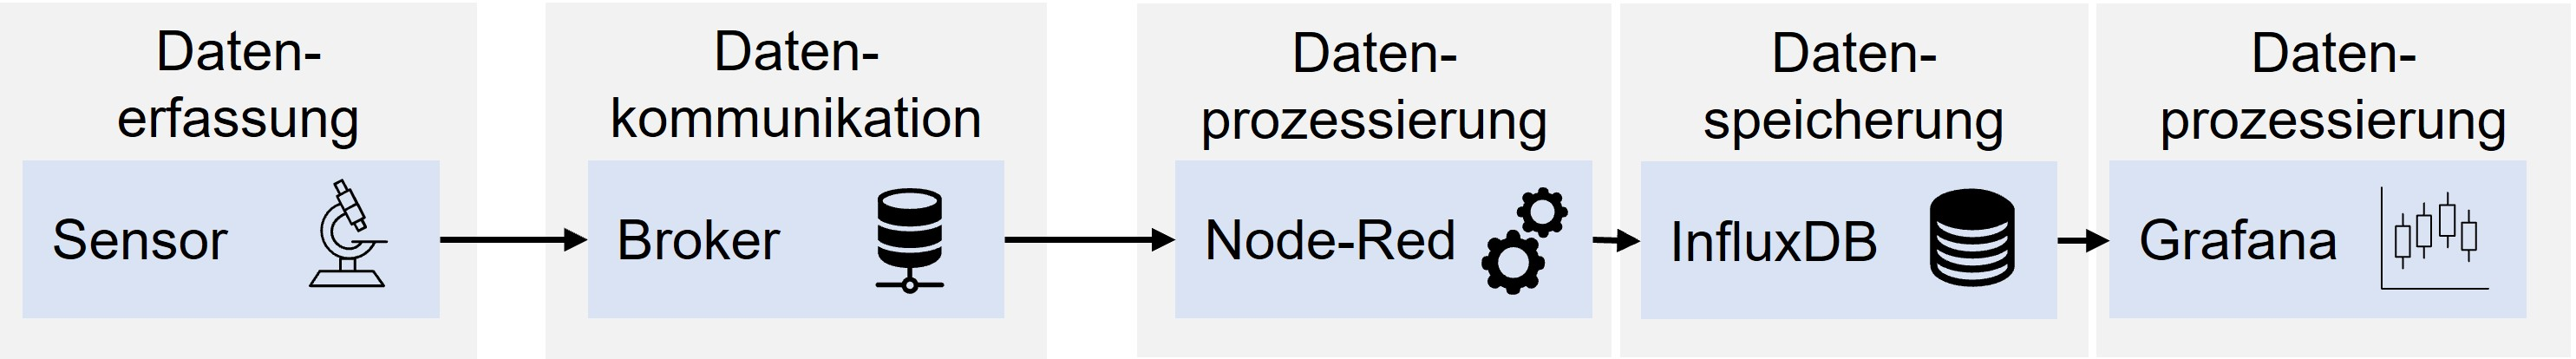
\includegraphics{images/mqtt-node-red-inffluxdb-grafana.jpg}

}

\caption{\label{fig-iotpipeline}Typischer IoT Datenfluss und
Verarbeitung über diverse Instanzen, von dem IoT Gerät mit Sensorik,
Datenkommunikation mit MQTT und dem MQTT Broker, zur Datenprozessierung
mit Node-Red, Datenspeicherung und und Visalisierung.}

\end{figure}%

Ziel dieser Übung ist es MQTT näher kennenzulernen und die MQTT
Kommunikation mit dem Raspberry Pi zu testen. MQTT ist ein
leichtgewichtiges Kommunikationsprotokoll, welches das
\emph{Publish-Subscribe} Muster verwendet und gut für die Anwendung in
IoT Projekten geeignet.

\section*{Übungsaufbau}\label{uxfcbungsaufbau-6}
\addcontentsline{toc}{section}{Übungsaufbau}

\markright{Übungsaufbau}

\begin{itemize}
\tightlist
\item
  Schliesse den Raspberry Pi an Monitor, Keyboard und Maus an oder
  verbinde Dich mit diesem über SSH (und SFTP).
\item
  Erstelle auf dem Raspberry Pi im \texttt{Documents} Ordner einen neuen
  Ordner \texttt{mqtt}, in welchem Du Änderungen und neue Dateien für
  diese Übung speichern kannst.
\item
  Schliesse den Sensor \textbf{BME688} an den Raspberry Pi über die
  Breakout Garden \textbf{I2C} Schnittstelle korrekt an (siehe
  \href{E01_Luftqualitaet.qmd}{E01 Luftqualität}), so dass die
  Beschriftung der Anschlüsse am Sensor und bei der Schnittstelle
  übereinstimmen.
\item
  Kontrolliere mit dem Befehl \texttt{i2cdetect\ -y\ 1} ob der Raspberry
  Pi mit dem Sensor verbunden ist. Der Sensor sollte auf der Adresse
  \texttt{0x76} erkannt werden.
\item
  Kontrolliere, ob die Library \texttt{sudo\ pip3\ install\ bme680}
  installiert ist mit
  \texttt{python\ -c\ "import\ sudo\ pip3\ install\ bme680"}.
  Installiere die Library mit
  \texttt{sudo\ pip3\ install\ sudo\ pip3\ install\ bme680} falls sie
  nicht installiert ist.
\item
  Wechsle in den Ordner \emph{Documents} und erstelle einen Ordner
  \emph{mqtt} für diese Übung.
\end{itemize}

\section*{Aufgabe 1: MQTT
kennenlernen}\label{aufgabe-1-mqtt-kennenlernen}
\addcontentsline{toc}{section}{Aufgabe 1: MQTT kennenlernen}

\markright{Aufgabe 1: MQTT kennenlernen}

Testen ob der \href{https://mosquitto.org}{Mosquitto} Broker und Clients
lokal auf dem Raspberry Pi funktionieren.


\includegraphics{images/mqtt-publish-subscribe.jpg}

Erstelle einen Subscriber der für das Topic \texttt{iot/temperature}
eine Subscription erstellt.

\begin{Shaded}
\begin{Highlighting}[]
\ExtensionTok{mosquitto\_sub} \AttributeTok{{-}h}\NormalTok{ 127.0.0.1 }\AttributeTok{{-}v} \AttributeTok{{-}t} \StringTok{\textquotesingle{}iot/temperature\textquotesingle{}}
\end{Highlighting}
\end{Shaded}

Öffne ein zweite Shell und erstelle einen Publisher für dasselbe Topic

\begin{Shaded}
\begin{Highlighting}[]
\ExtensionTok{mosquitto\_pub} \AttributeTok{{-}h}\NormalTok{ 127.0.0.1 }\AttributeTok{{-}t} \StringTok{\textquotesingle{}iot/temperature\textquotesingle{}} \AttributeTok{{-}m} \StringTok{\textquotesingle{}Aussentemperatur: 22° Celsius\textquotesingle{}}
\end{Highlighting}
\end{Shaded}

\begin{boxtitle}{Excercise}{colPrimary}

\begin{itemize}
\tightlist
\item
  Teste nun den MQTT mit unterschiedlichen Topics und Nachrichten.
\item
  Teste einen weiteren Mosquitto Server auf einem anderen Raspberry Pi
  und teste die Kommunikation. Hierbei muss die IP Adresse entsprechend
  angepasst werden.
\end{itemize}

\end{boxtitle}

Falls der Mosquitto Brokers und Clients nicht installiert sind, können
diese mit folgenden Befehlen installiert werden.

\begin{Shaded}
\begin{Highlighting}[]
\FunctionTok{sudo}\NormalTok{ apt install mosquitto }\AttributeTok{{-}y}
\FunctionTok{sudo}\NormalTok{ apt install mosquitto{-}clients }\AttributeTok{{-}y}
\FunctionTok{sudo}\NormalTok{ systemctl enable mosquitto.service}
\end{Highlighting}
\end{Shaded}

\begin{boxtitle}{Hinweis}{colPrimary}

\href{https://apps.microsoft.com/detail/9NBLGGH55JZG}{MQTTBox} und
\href{https://mqtt-explorer.com}{MQTT Explorer} sind zwei MQTT Clients,
die für die Entwicklung und das Testen von MQTT Applikationen verwendet
werden können. Jedoch scheinen diese nicht mehr oder eher sporadisch
weiterentwickelt zu werden.

\end{boxtitle}

\section*{Aufgabe 2: MQTT mit Python
verwenden}\label{aufgabe-2-mqtt-mit-python-verwenden}
\addcontentsline{toc}{section}{Aufgabe 2: MQTT mit Python verwenden}

\markright{Aufgabe 2: MQTT mit Python verwenden}

Nun verwenden wir die Bibliothek \texttt{paho-mqtt} in Python um MQTT zu
verwenden. Folgende zwei Code Snippets zeigen wie ein Publisher und
Subscriber in Python implementiert werden können.


\includegraphics{images/mqtt-sensor-subscribe.jpg}

\textbf{Script 1:} \texttt{mqtt\_sub.py} - Subscriber

\phantomsection\label{annotated-cell-30}%
\begin{Shaded}
\begin{Highlighting}[]
\ImportTok{import}\NormalTok{ paho.mqtt.client }\ImportTok{as}\NormalTok{ mqtt }
\NormalTok{ip }\OperatorTok{=} \StringTok{"127.0.0.1"} \hspace*{\fill}\NormalTok{\circled{1}}
\NormalTok{topic }\OperatorTok{=} \StringTok{"iot/temperature"} \hspace*{\fill}\NormalTok{\circled{2}}

\CommentTok{\# Callback Funktion für den Verbindungsaufbau}
\KeywordTok{def}\NormalTok{ on\_connect(client, userdata, flags, rc): }\hspace*{\fill}\NormalTok{\circled{3}}
    \BuiltInTok{print}\NormalTok{(}\StringTok{"Connected {-} code: "}\OperatorTok{+}\BuiltInTok{str}\NormalTok{(rc)) }
\NormalTok{    client.subscribe(topic) }\hspace*{\fill}\NormalTok{\circled{4}}
  
\CommentTok{\# Callback Funktion für eingehende Nachrichten}
\KeywordTok{def}\NormalTok{ on\_message(client, userdata, msg): }\hspace*{\fill}\NormalTok{\circled{5}}
    \BuiltInTok{print}\NormalTok{(msg.topic}\OperatorTok{+}\StringTok{" "}\OperatorTok{+}\BuiltInTok{str}\NormalTok{(msg.payload)) }
  
\CommentTok{\# Erstellen des MQTT Clients}
\NormalTok{client }\OperatorTok{=}\NormalTok{ mqtt.Client() }\hspace*{\fill}\NormalTok{\circled{6}}
\NormalTok{client.on\_connect }\OperatorTok{=}\NormalTok{ on\_connect }
\NormalTok{client.on\_message }\OperatorTok{=}\NormalTok{ on\_message }
\NormalTok{client.}\ExtensionTok{connect}\NormalTok{(ip, }\DecValTok{1883}\NormalTok{, }\DecValTok{60}\NormalTok{) }\hspace*{\fill}\NormalTok{\circled{7}}
\NormalTok{client.loop\_forever() }
\end{Highlighting}
\end{Shaded}

\begin{description}
\tightlist
\item[\circled{1}]
IP Adresse des MQTT Brokers
\item[\circled{2}]
Topic auf welches der Subscriber hört
\item[\circled{3}]
Callback Funktion on\_connect wird ausgeführt, wenn die Verbidnung steht
\item[\circled{4}]
Subscription für das Topic
\item[\circled{5}]
Callback Funktion on\_publish wird ausgeführt, wenn eine Nachricht
empfangen (publish) wird
\item[\circled{6}]
Erstellen eines MQTT Clients und Zuweisung der Callback Funktionen
\item[\circled{7}]
Verbindung zum MQTT Broker herstellen und auf eingehende Nachrichten
warten (loop\_forever)
\end{description}

\textbf{Script 2: }\texttt{mqtt\_pub.py} - Publisher

\phantomsection\label{annotated-cell-31}%
\begin{Shaded}
\begin{Highlighting}[]
\ImportTok{import}\NormalTok{ paho.mqtt.publish }\ImportTok{as}\NormalTok{ publish }
\NormalTok{ip }\OperatorTok{=} \StringTok{"127.0.0.1"} \hspace*{\fill}\NormalTok{\circled{1}}
\NormalTok{topic }\OperatorTok{=} \StringTok{"iot/temperature"} 
\NormalTok{publish.single(topic, }\StringTok{"22.0"}\NormalTok{, hostname}\OperatorTok{=}\NormalTok{ip, port}\OperatorTok{=}\DecValTok{1883}\NormalTok{) }\hspace*{\fill}\NormalTok{\circled{2}}
\end{Highlighting}
\end{Shaded}

\begin{description}
\tightlist
\item[\circled{1}]
IP Adresse des MQTT Brokers und Topic definieren
\item[\circled{2}]
Nachricht mit Topic an den MQTT Broker (ip,port) senden
\end{description}

\begin{boxtitle}{Excercise}{colPrimary}

\begin{itemize}
\tightlist
\item
  Speichere die beiden Dateien \texttt{mqtt\_pub.py} und
  \texttt{mqtt\_sub.py} im Ordner \texttt{mqtt} ab.
\item
  (Optional: Passe die IP Adresse des MQTT Brokers an, falls ein anderer
  MQTT Broker genutzt werden soll.)
\item
  Öffne zwei Terminals und führe diese mit
  \texttt{python3\ mqtt\_pub.py} und \texttt{python3\ mqtt\_sub.py} aus.
\end{itemize}

\end{boxtitle}

Falls die Library paho-mqtt nicht installiert ist, kann diese mit
\texttt{sudo\ pip3\ install\ paho-mqtt} installiert werden.

\section*{Aufgabe 3: Sensordaten mit MQTT
übertragen}\label{aufgabe-3-sensordaten-mit-mqtt-uxfcbertragen}
\addcontentsline{toc}{section}{Aufgabe 3: Sensordaten mit MQTT
übertragen}

\markright{Aufgabe 3: Sensordaten mit MQTT übertragen}

Passe nun das Script \texttt{mqtt\_pub.py} an, so dass die Temperatur
vom Sensor \texttt{BME688} ausgelesen und über MQTT übertragen wird. Die
Temperatur soll alle 10 Sekunden übertragen werden. Nutze hierfür das
Script zum Auslesen der Sensordaten aus der Übung
\href{E01_Luftqualitaet.qmd}{E01 Luftqualität} und passe dieses an.

\begin{boxtitle}{Excercise}{colPrimary}

\begin{itemize}
\tightlist
\item
  Speichere das \texttt{mqtt\_pub.py} als \texttt{mqtt\_pub\_bme688.py}
  im Ordner \texttt{mqtt} ab.
\item
  Ergänze das Script um die Funktionen zum auslesen der Temperatur des
  BME688 Sensors.
\item
  Ergänze das Script für das Auslesen der Luftfeuchtigkeit und Luftdruck
  und ergänze die topics mit \texttt{iot/humidity} und
  \texttt{iot/pressure}.
\item
  Erweitere das Script \texttt{mqtt\_sub.py} um die Subscription für die
  Topics \texttt{iot/humidity} und \texttt{iot/pressure} und speichere
  es als \texttt{mqtt\_sub\_bme688.py} ab.
\item
  Öffne zwei Terminals und führe diese mit
  \texttt{python3\ mqtt\_pub\_bme688.py} und
  \texttt{python3\ mqtt\_sub\_bme688.py} aus.
\end{itemize}

\end{boxtitle}

\section*{Aufgabe 4: MQTT mit Node-RED
verwenden}\label{aufgabe-4-mqtt-mit-node-red-verwenden}
\addcontentsline{toc}{section}{Aufgabe 4: MQTT mit Node-RED verwenden}

\markright{Aufgabe 4: MQTT mit Node-RED verwenden}

Node-Red\index{Node-Red} ist ein grafisches Entwicklungswerkzeug für
IoT, ein low-code Tool für \emph{event-driven applications}. Es bietet
eine browserbasierte und datenstromorientierte ``Flow'' Programmierung
für die Verarbeitung von Sensordaten (ähnlich wie FME oder graphische
Modellierungswerkzeuge in GIS). Die Implementation von Node-Red ist in
JavaScript und basiert auf node.js. Datenverarbeitungsflows können
gespeichert und wiederverwendet werden. Im Arbeitsbereich
(Abbildung~\ref{fig-noderedmqttflow}) können sogenannte Nodes, die
unterschiedliche Funktionen erfüllen, zu einem Daten-``Flow'' werden.
Nodes können auch selbst erstellt werden. Es gibt eine Vielzahl von
Nodes, die von der Community entwickelt wurden, die über den Node-Red
Palette Manager installiert werden können. Core Nodes von Node-Red sind:

\begin{itemize}
\tightlist
\item
  \textbf{Inject Node}: Kann einen Flow über den Button direkt auslösen
  oder in regelmässigen Abständen mit Zeitstempel oder vordefinierten
  Nachrichten (msg) senden.
\item
  \textbf{Debug Node}: Kann die
  \href{https://nodered.org/docs/user-guide/messages}{Nachrichten} (msg)
  in Debug Sidebar anzeigen lassen.
\item
  \textbf{Function Node}: Kann mit JavaScript
  \href{https://nodered.org/docs/user-guide/writing-functions}{Funktionen}
  den Inhalt der Nachrichten (msg) verändern.
\item
  \textbf{Change Node}: Ermöglicht das Ändern von Eigenschaften einer
  Nachricht (ohne den Funktion Node zu nützen) um beispielsweise
  Eigenschaften zu setzen, ändern oder löschen.
\item
  \textbf{Switch Node}: Kann Nachrichten (msg) anhand von Regeln
  auswerten in verschiedene Ausgänge leiten (wie ein Switch Case in der
  Programmierung).
\item
  \textbf{Template Node}: Kann über Eigenschaften einer Nachricht und
  einer Vorlage (Template) neue Nachricht nach Vorlage erstellen:
  \texttt{Nachricht:\ \{\{payload\}\}!} wird
  \texttt{Nachricht:\ 1570439577309\ !}.
\end{itemize}

Node-Red kann über den Browser auf dem Raspberry Pi oder via Laptop
gestartet werden. Öffne den Browser und gebe die IP Adresse des
Raspberry Pi mit dem Port 1880 ein:
\texttt{http://\textless{}ip-adresse\textgreater{}:1880}. Führt nun das
Kurztutorial zu Node-Red aus:
\href{https://nodered.org/docs/getting-started/first-flow}{Node-Red
Getting Started: First Flow}. In diesem Tutorial wird ein Flow erstellt,
der eine Nachricht mit einem Zeitstempel ausgibt.

\begin{figure}

\centering{

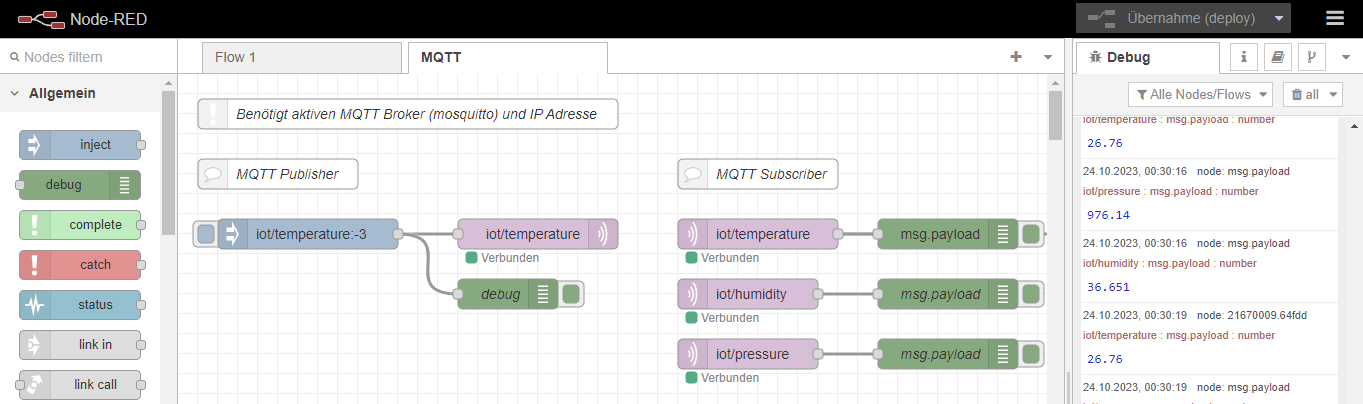
\includegraphics{images/node-red_mqtt_flow.png}

}

\caption{\label{fig-noderedmqttflow}Node-Red Flow der Daten in das Topic
\emph{iot/temperature} published, und Nachrichten aus dem Topic
\emph{iot/temperature} subscribed.}

\end{figure}%

\begin{boxtitle}{Excercise}{colPrimary}

Erstelle einen Flow der Nachrichten an den MQTT Broker senden und
Nachrichten vom MQTT Broker empfangen kann.

\begin{enumerate}
\def\labelenumi{\arabic{enumi}.}
\tightlist
\item
  Füge hierfür einen Inject Node, einen Debug Node und einen MQTT Output
  Node hinzu. Öffne die Einstellungen des MQTT Output Nodes (siehe
  Abbildung~\ref{fig-noderedmqttnodesetup}) und setze die IP Adresse des
  MQTT Brokers und das Topic auf \texttt{iot/temperature}. Starte den
  Flow und überprüfe, ob die Nachrichten an den MQTT Broker gesendet
  werden.
\item
  Erstelle nun einen weiteren Flow, der die Nachrichten vom MQTT Broker
  empfängt und in der Debug Sidebar anzeigt. Füge hierfür einen MQTT
  Input Node (siehe Abbildung~\ref{fig-noderedmqttnodesetup}) und einen
  Debug Node hinzu. Öffne die Einstellungen des MQTT Input Nodes und
  setze die IP Adresse des MQTT Brokers und das Topic auf
  \texttt{iot/temperature}. Starte den Flow und überprüfe, ob die
  Nachrichten vom MQTT Broker empfangen werden.
\item
  Ergänze den Flow um einen MQTT Input Node für die Topics
  \texttt{iot/humidity} und \texttt{iot/pressure} und je einen Debug
  Node. Starte den Flow und überprüfe, ob die Nachrichten vom MQTT
  Broker empfangen werden.
\end{enumerate}

\end{boxtitle}

\begin{figure}

\centering{

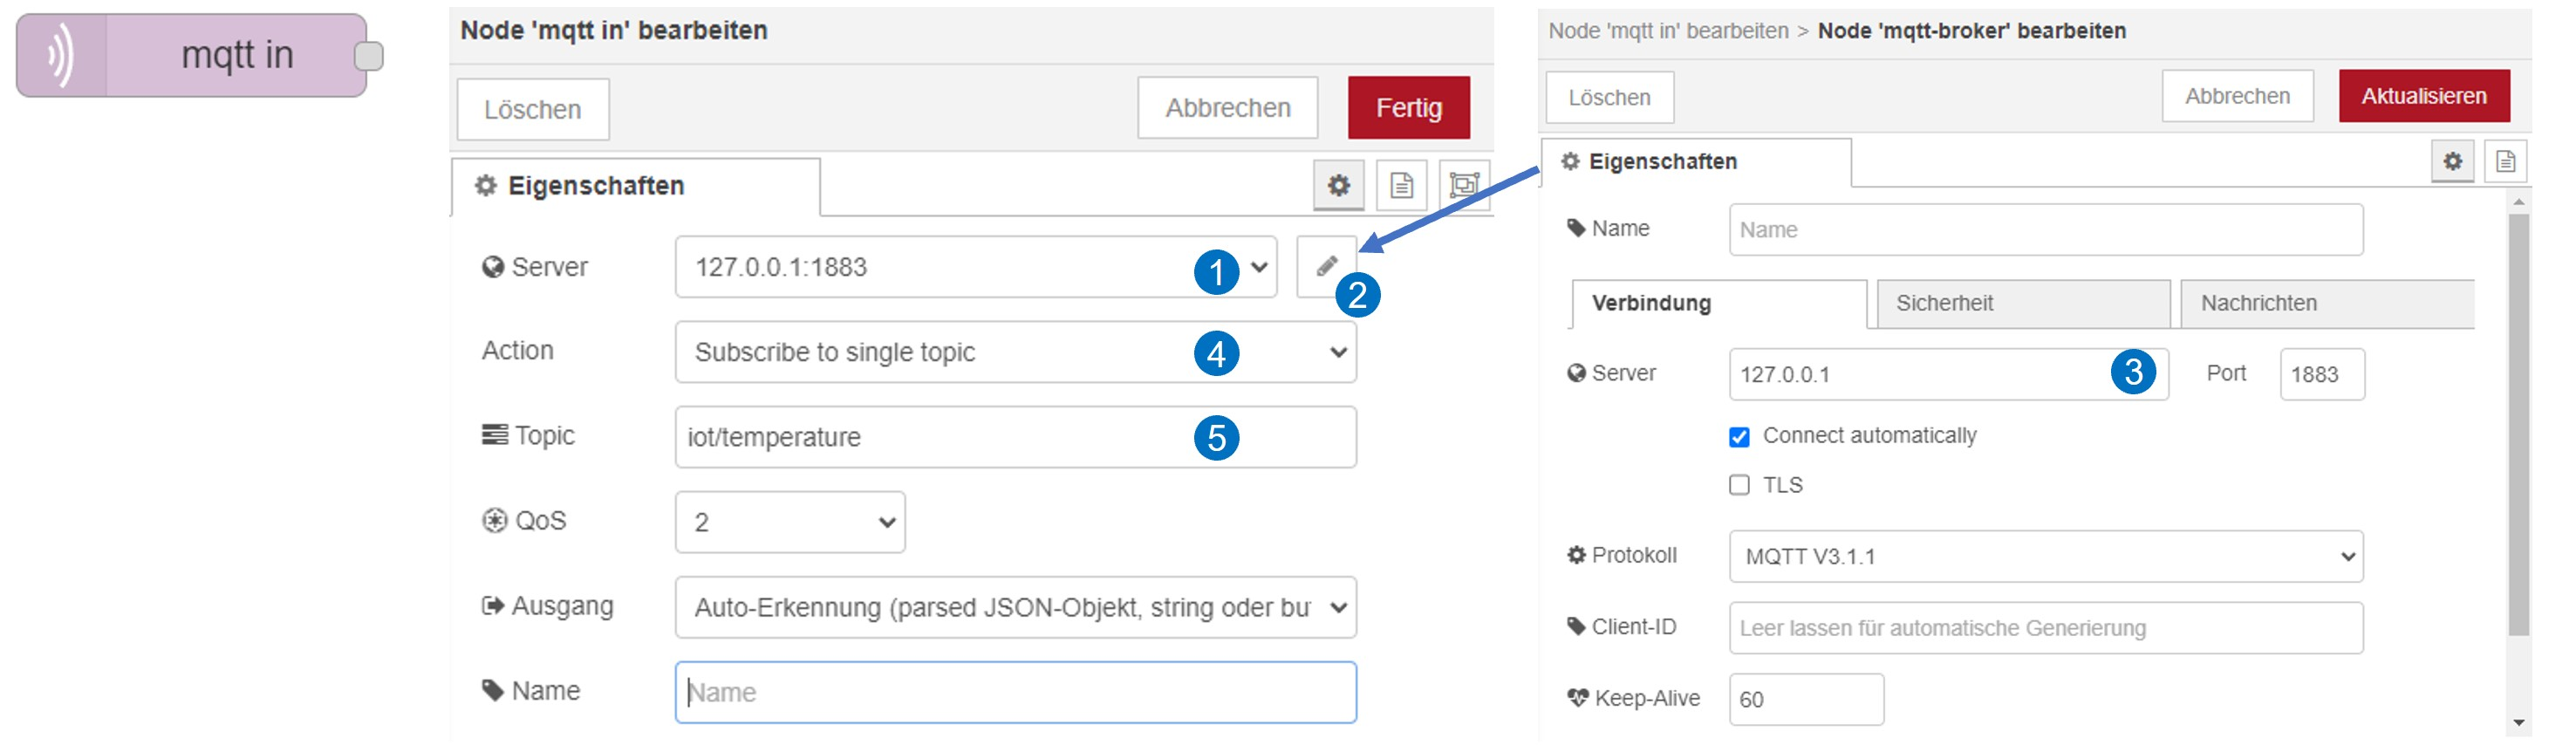
\includegraphics{images/node-red_mqtt_setup.jpg}

}

\caption{\label{fig-noderedmqttnodesetup}Node-Red MQTT Node
Einstellungen setzen, (1) Name angeben, (2) Server Einstellungen öffnen
und (3) IP Adresse des MQTT Brokers setzen, (4) subscribe to single
topic wählen und (5) Topic \texttt{iot/temperature} setzen.}

\end{figure}%

\begin{boxtitle}{Hinweis}{colPrimary}

Flows stoppen: Um einen Flow in der Ausführung zu stoppen, kann dieser
über den Tab (rechte Maustaste) Flow deaktiviert werden (disable flow)
und mit einem erneuten Übernehmen (Deploy) wird der Flow gestoppt.

\end{boxtitle}

\section*{Aufgabe 5: Node-Red MQTT mit InfluxDB
verwenden}\label{aufgabe-5-node-red-mqtt-mit-influxdb-verwenden}
\addcontentsline{toc}{section}{Aufgabe 5: Node-Red MQTT mit InfluxDB
verwenden}

\markright{Aufgabe 5: Node-Red MQTT mit InfluxDB verwenden}

InfluxDB ist die Datenbank, die für die Erfassung, Speicherung,
Verarbeitung und Visualisierung von Zeitreihendaten entwickelt wurde.
Zeitreihendaten sind Datenpunkt, die in zeitlicher Sequenz erfasst
wurden und bestehen in der Regele aus aufeinanderfolgenden Messungen aus
derselben Quelle, wie beispielsweise die Temperaturdaten des BME688.
InfluxDB organisiert die Zeitreihendaten in Buckets (anstatt
Datenbanken) und Messungen. Ein Bucket kann mehrere Messungen enthalten,
wobei Messungen Felder und Tags enthalten können (influxdata 2023). Eine
Messung ist enthält Felder mit key-value Paaren von Messwerten, die sich
über die Zeit ändern. Tags sind key-value Paare, die sich nicht über die
Zeit ändern und für die Filterung und Gruppierung verwendet werden
können.

Das Tutorial
\href{https://docs.influxdata.com/influxdb/v2/get-started/}{Getting
Started} zeigt die ersten Schritte mit InfluxDB.


\includegraphics{images/mqtt-sensor-broker-influxdb.jpg}

Die graphische Oberfläche von InfluxDB kann über den Browser auf dem
Raspberry Pi oder via Laptop gestartet werden.

Öffnet nun den Browser und gebe die IP Adresse des Raspberry Pi mit dem
Port 8086 ein: \texttt{http://\textless{}ip-adresse\textgreater{}:8086}.
Erstellt über die linke Menuleiste unter \emph{Load Data} einen neuen
Bucket mit dem Namen \texttt{iot}, falls dieser nicht schon existiert.
Kopiert unter \emph{load Data / API Tokens} den Token für den Zugang zur
Datenbank.

Diese Angaben (\emph{bucket} und \emph{API Token}) werden für den
InfluxDB Node in Node-Red benötigt. Die Einstellungen des InfluxDB Node
benötigen die Angaben, wohin die Daten in der Datenbank gespeichert
werden (links in Abbildung~\ref{fig-noderedinfluxdb}) mit Angaben zum
Bucket (Datenbankname), Organisation\footnote{wird bei der Erstellung
  der Datenbank definiert} und measurement und die Serververbindung
(rechts in Abbildung~\ref{fig-noderedinfluxdb}) mit der IP Adresse und
das Token für den Zugang zur Datenbank.

\begin{boxtitle}{Hinweis}{colPrimary}

Falls keine Nodes für InfluxDB in Node-Red vorhanden sind, kann die
Erweiterung \texttt{node-red-contrib-influxdb} über das Hauptmenu
\emph{Palette verwalten} im Tab \emph{Installation} installiert werden.

\end{boxtitle}

\begin{figure}

\centering{

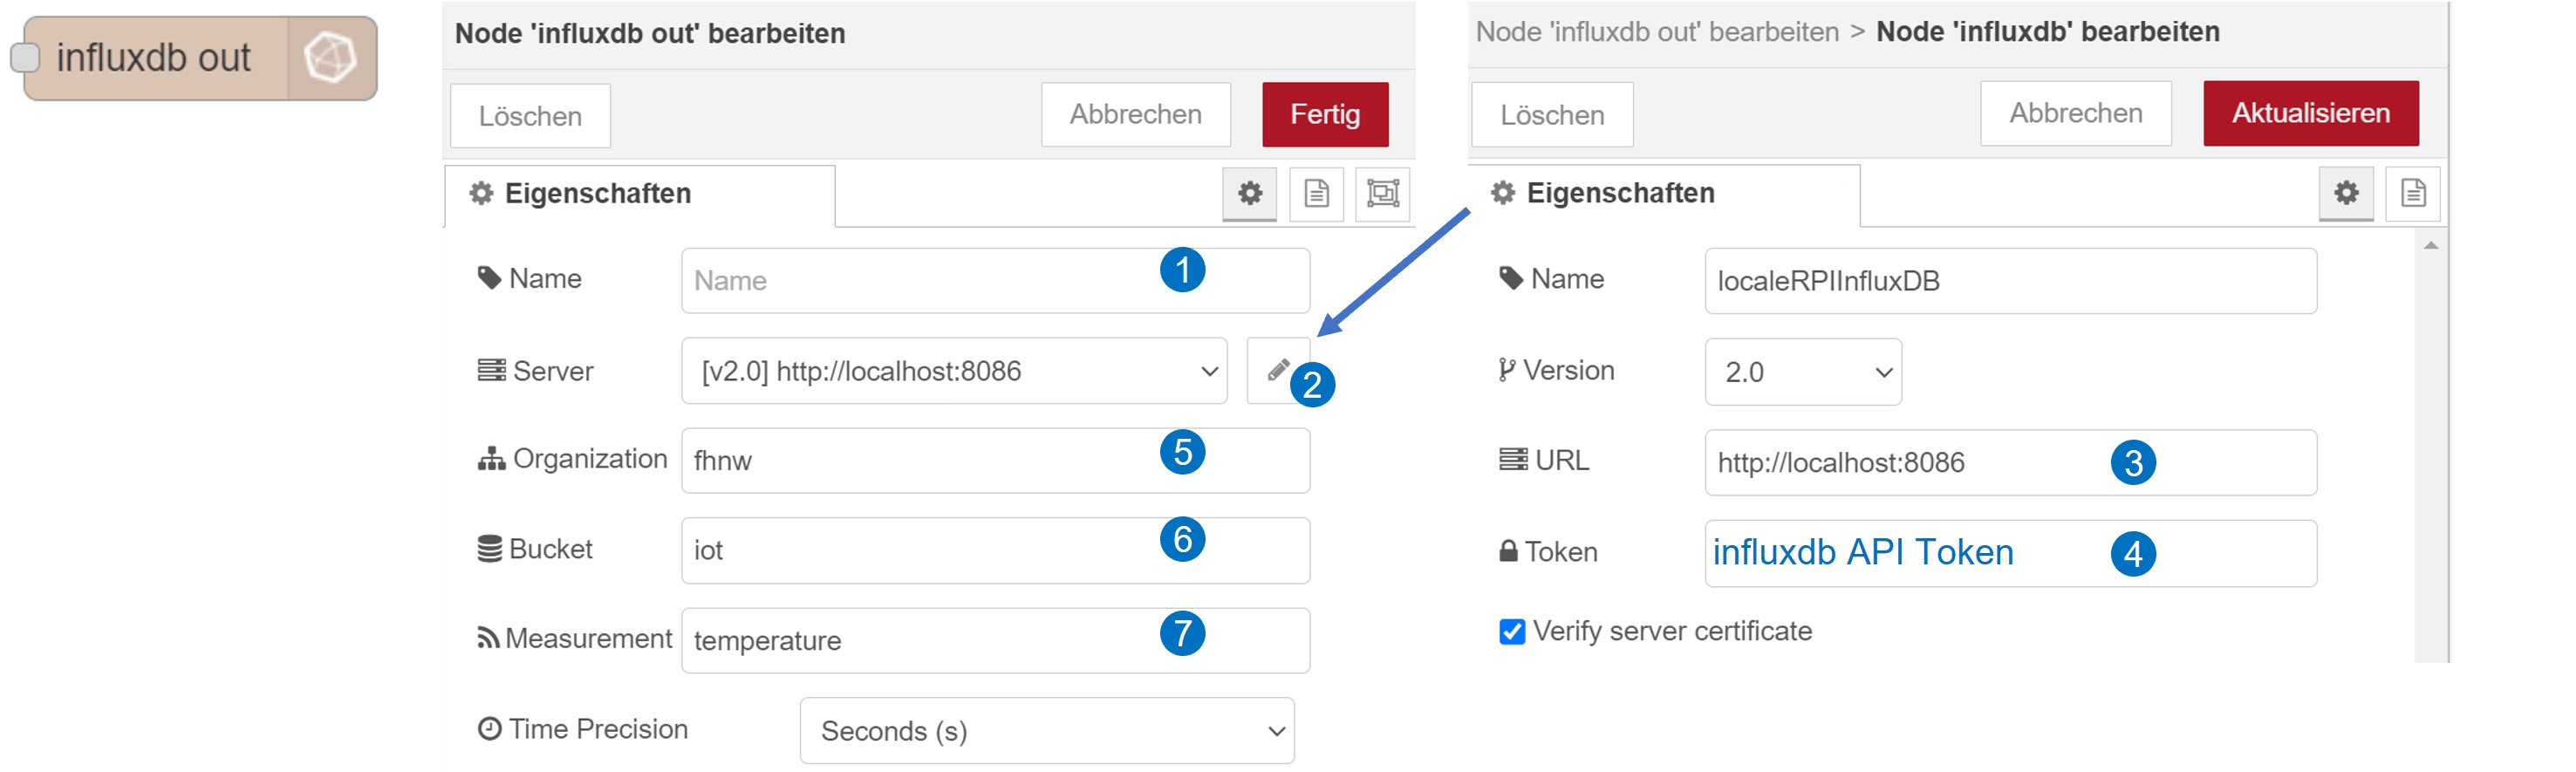
\includegraphics{images/node-red_influxdb_setup.jpg}

}

\caption{\label{fig-noderedinfluxdb}Einstellungen der InflxDB Nodes in
Node-Red, links: Einstellungen zur Datenbank (1) mit Angaben zur
Organisation (5), Bucket (6) und Namen der Messung \emph{measurement}
(7), rechts: Einstellungen zur Datenbankverbindung (2) mit der URL und
Port der InfluxDB (3) und dem API Token (4), für den Zugang zur
Datenbank.}

\end{figure}%

Die Messwerte können direkt in die InfluxDB geschrieben werden, jedoch
fehlen da noch die Tags, die für die Filterung und Gruppierung verwendet
werden können. Diese können über den Change Node hinzugefügt werden, wie
in Abbildung~\ref{fig-noderedpayload} gezeigt. Hierbei wird der Wert der
Payload in ein Feld mit dem Namen \emph{temperature} geschrieben und die
Tags \emph{device} und \emph{sensor} werden hinzugefügt. Dieselbe
Struktur kann alternativ auch mit dem Function Node erstellt werden,
siehe Abbildung~\ref{fig-noderedpayload} rechts. Hierbei wird der Wert
der Payload in ein Feld mit dem Namen \emph{temperature} geschrieben und
die Tags \emph{device} und \emph{sensor} werden hinzugefügt. Die
Bezeichnung der Messung \emph{temperature} wird im InfluxDB Node
definiert oder kann im Function Node überschrieben werden.

\begin{figure}

\centering{

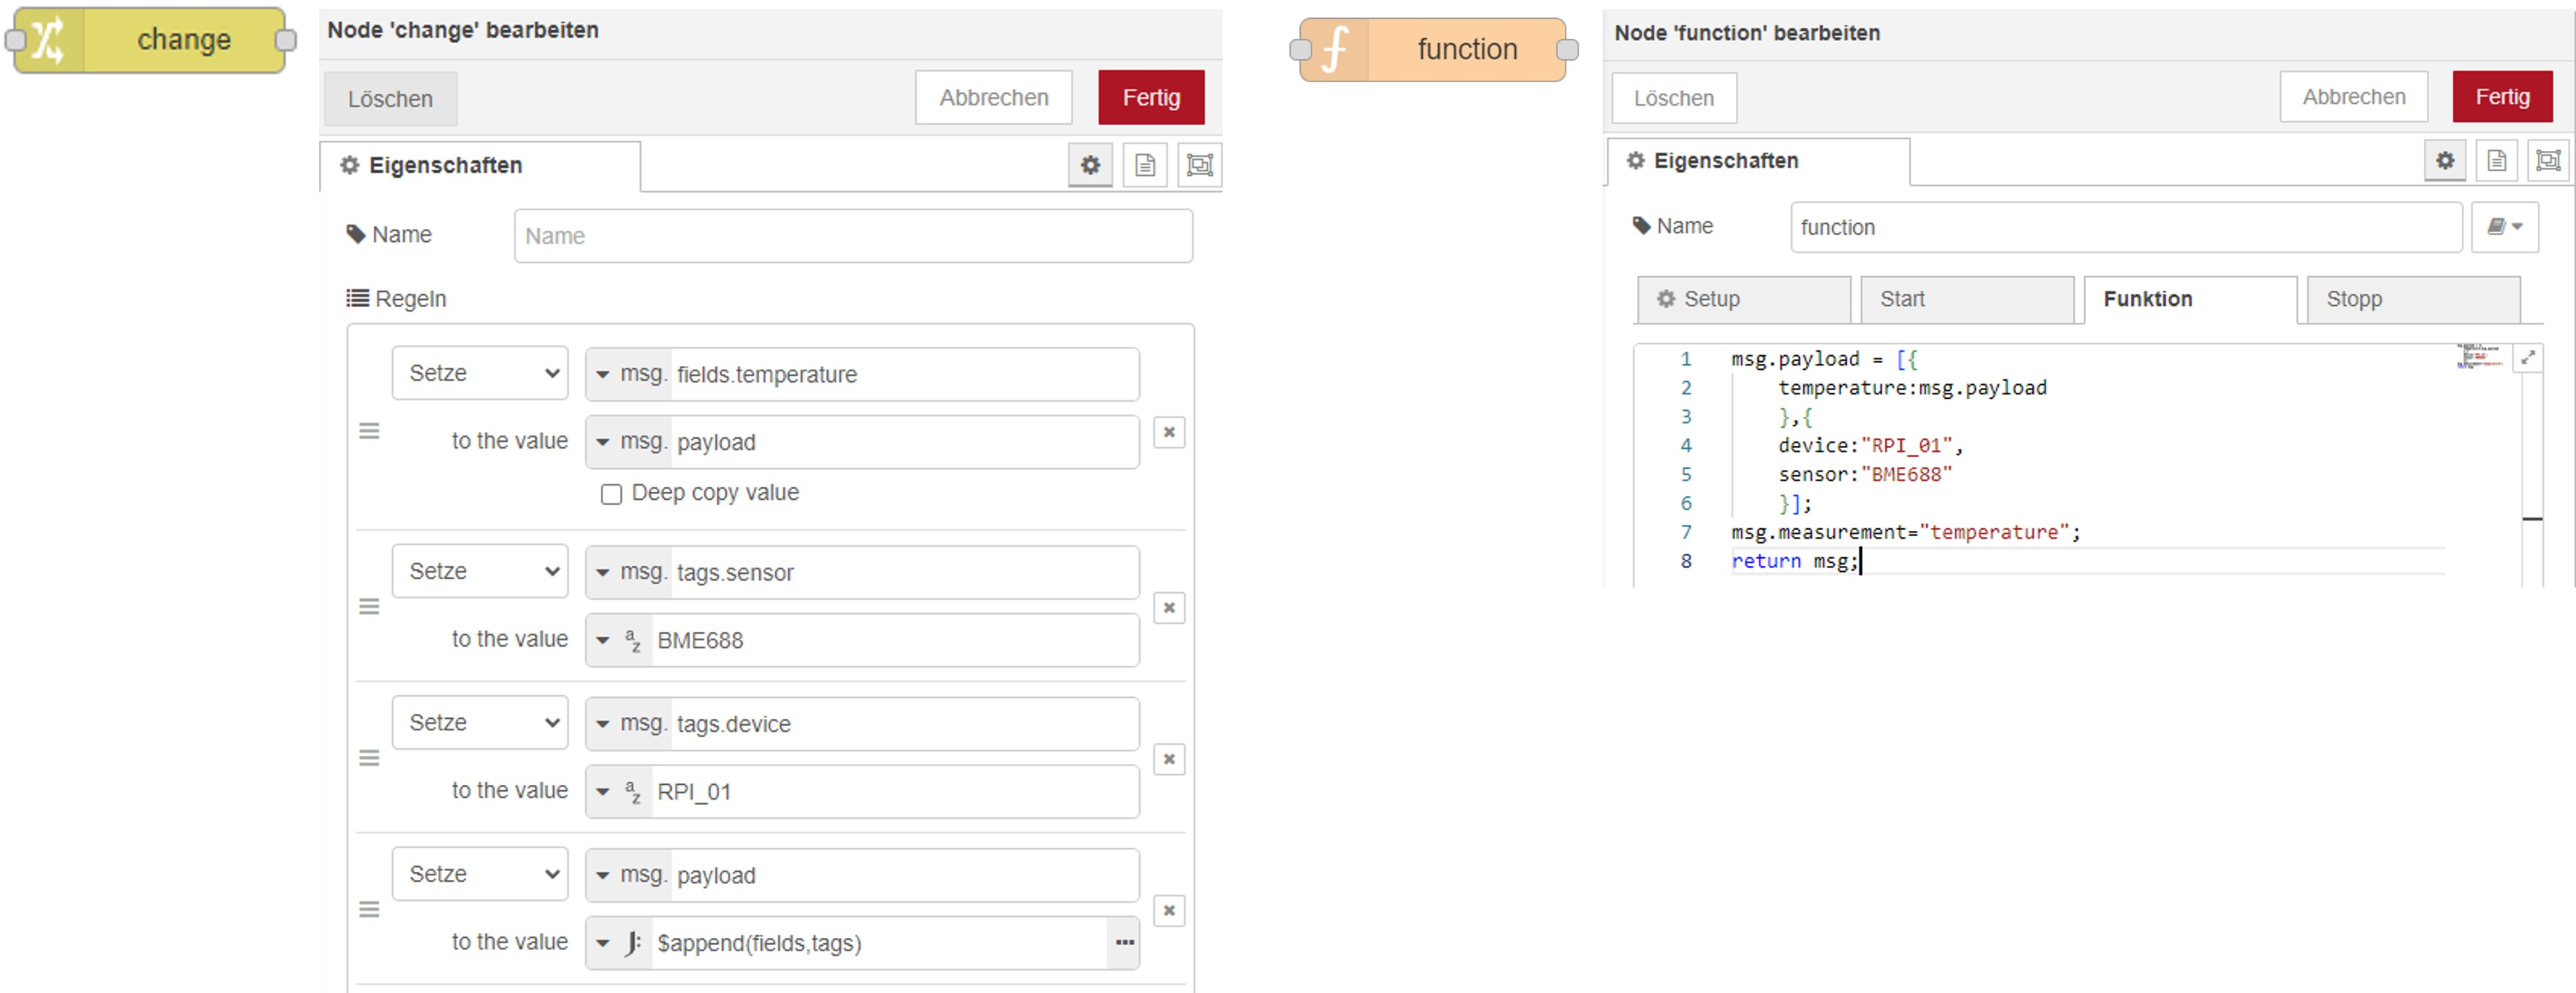
\includegraphics{images/node-red_influxdb_change_function_node.jpg}

}

\caption{\label{fig-noderedpayload}Über den Change Node, wie auch den
Function Node kann mit JavaScript der Inhalt der Payload verändert
werden und diesen für den Import in die InfluxDB angepasst werden.}

\end{figure}%

\phantomsection\label{annotated-cell-32}%
\begin{Shaded}
\begin{Highlighting}[]
\NormalTok{msg}\OperatorTok{.}\AttributeTok{payload} \OperatorTok{=}\NormalTok{ [\{ }
    \DataTypeTok{temperature}\OperatorTok{:}\NormalTok{msg}\OperatorTok{.}\AttributeTok{payload} \hspace*{\fill}\NormalTok{\circled{1}}
\NormalTok{\}}\OperatorTok{,}\NormalTok{ \{ }\DataTypeTok{device}\OperatorTok{:}\StringTok{"RPI\_01"}\OperatorTok{,}\DataTypeTok{ sensor}\OperatorTok{:}\StringTok{"BME688"}\NormalTok{ \}]}\OperatorTok{;} \hspace*{\fill}\NormalTok{\circled{2}}
\NormalTok{msg}\OperatorTok{.}\AttributeTok{measurement}\OperatorTok{=}\StringTok{"temperature"}\OperatorTok{;} \hspace*{\fill}\NormalTok{\circled{3}}
\ControlFlowTok{return}\NormalTok{ msg}\OperatorTok{;}
\end{Highlighting}
\end{Shaded}

\begin{description}
\tightlist
\item[\circled{1}]
Werte der Payload in Payloadstruktur für die InfluxDB schreiben
\item[\circled{2}]
Tags der Messung zuweisen
\item[\circled{3}]
Optional \emph{measurement} kann im InfluxDB Node oder im
Funktionsknoten definiert werden
\end{description}

InfluxDB bietet über das Menu \emph{Data Explorer} eine einfache
Möglichkeit die Daten zu visualisieren. Der Query Builder
(Abbildung~\ref{fig-influxdbdataexplorer}) hilft bei der Erstellung von
Abfragen mit der über die Fields und Tags gefiltert werden kann, die
dann über den Button \emph{Submit} ausgeführt und dargestellt werden
können. Die erstellte Query kann über den \emph{Script Editor}
(Abbildung~\ref{fig-influxdbdataexplorer}) angezeigt werden.

\begin{figure}

\centering{

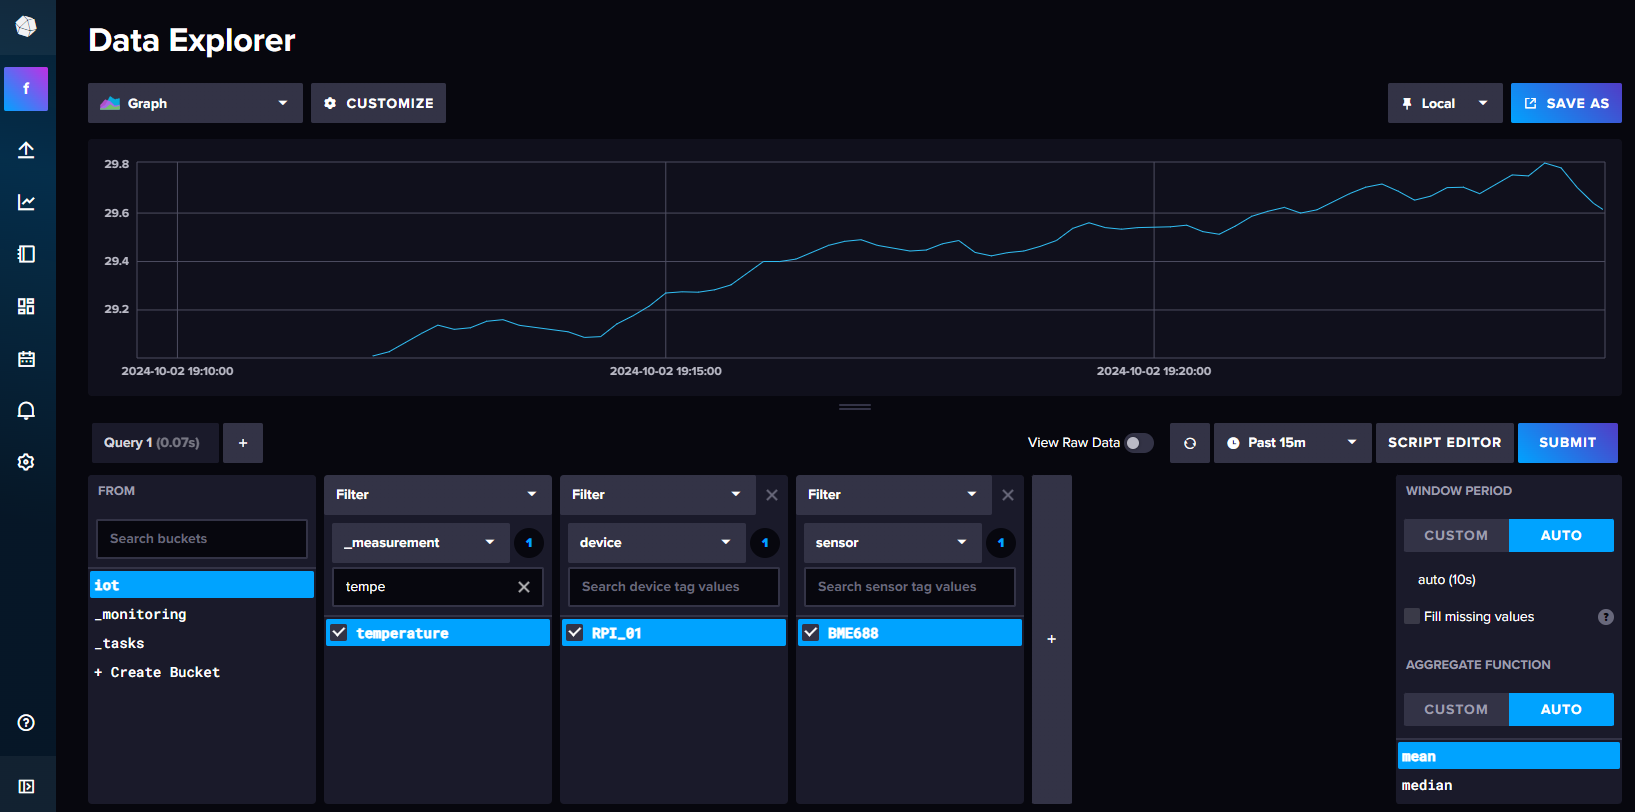
\includegraphics{images/influxdb_data_explorer.png}

}

\caption{\label{fig-influxdbdataexplorer}Über den \emph{Data Explorer}
können in InfluxDB einfach Abfragen zusammengestellt und über
\emph{submit} visualisiert werden}

\end{figure}%

\begin{boxtitle}{Excercise}{colPrimary}

\begin{itemize}
\tightlist
\item
  Erstellt nun einen Flow der die Nachrichten des Topics
  \texttt{iot/temperature} vom MQTT Broker empfängt und in die InfluxDB
  schreibt.
\item
  Erstellt erst einen flow der nur die Nachrichten ohne Tags in die
  InfluxDB schreibt
\item
  Ergänzt den Flow mit einem Change oder Function Node um die Tags
  \emph{device} und \emph{sensor} hinzuzufügen.
\item
  Visualisiert den Temperaturverlauf des BME688 in der InfluxDB mit dem
  \emph{Data Explorer} und studiert die Flux Abfragesprache.
\item
  Erstellt einen Flow der die Nachrichten der Topics
  \texttt{iot/humidity} und \texttt{iot/pressure} vom MQTT Broker
  empfängt und in die InfluxDB schreibt.
\item
  (Optional) erstellt im Menu \emph{Dashboard} eine Visualisierung der
  Messwerte.
\end{itemize}

\end{boxtitle}

\section*{Aufgabe 6: InfluxDB mit Grafana
verwenden}\label{aufgabe-6-influxdb-mit-grafana-verwenden}
\addcontentsline{toc}{section}{Aufgabe 6: InfluxDB mit Grafana
verwenden}

\markright{Aufgabe 6: InfluxDB mit Grafana verwenden}

Grafana ist eine Open-Source Anwendung für die Darstellung von Daten aus
den unterschiedlichsten Messquellen, wie Postgres, SQLite oder InfluxDB.
In dieser Übung wird Grafana mit der InfluxDB Datenbank verwendet.

Öffnet nun den Browser und gebt die IP Adresse des Raspberry Pi mit dem
Port 3000 ein: \texttt{http://\textless{}ip-adresse\textgreater{}:3000}.
Unter Connections / Data Sources können Grafana Datenquellen hinzugefügt
werden, wählt nun \emph{InfluxDB} um Grafana mit der InfluxDB zu
verbinden. Setzt folgende Einstellungen
(Abbildung~\ref{fig-grafanainfluxdb}) und speichert diese:

\begin{itemize}
\tightlist
\item
  \emph{Query Language}: Wählt in den Einstellungen zu \emph{Query
  Language} die Abfragesprache \texttt{Flux}.
\item
  \emph{HTTP}: Setzt die IP Adresse des Raspberry Pi und den Port 8086:
  \texttt{http://localhost:8086}.
\item
  \emph{Auth}: aktiviert \emph{Basic Auth}
\item
  \emph{Basic Auth Details}: Setzt den InfluxDB Benutzer und das
  Passwort für die InfluxDB
\item
  \emph{InfluxDB Details}: Setzt die InfluxDB Organisation \emph{fhnw},
  den \emph{API Token}, und den InfluxDB Bucket \emph{iot}.
\end{itemize}

\begin{figure}

\centering{

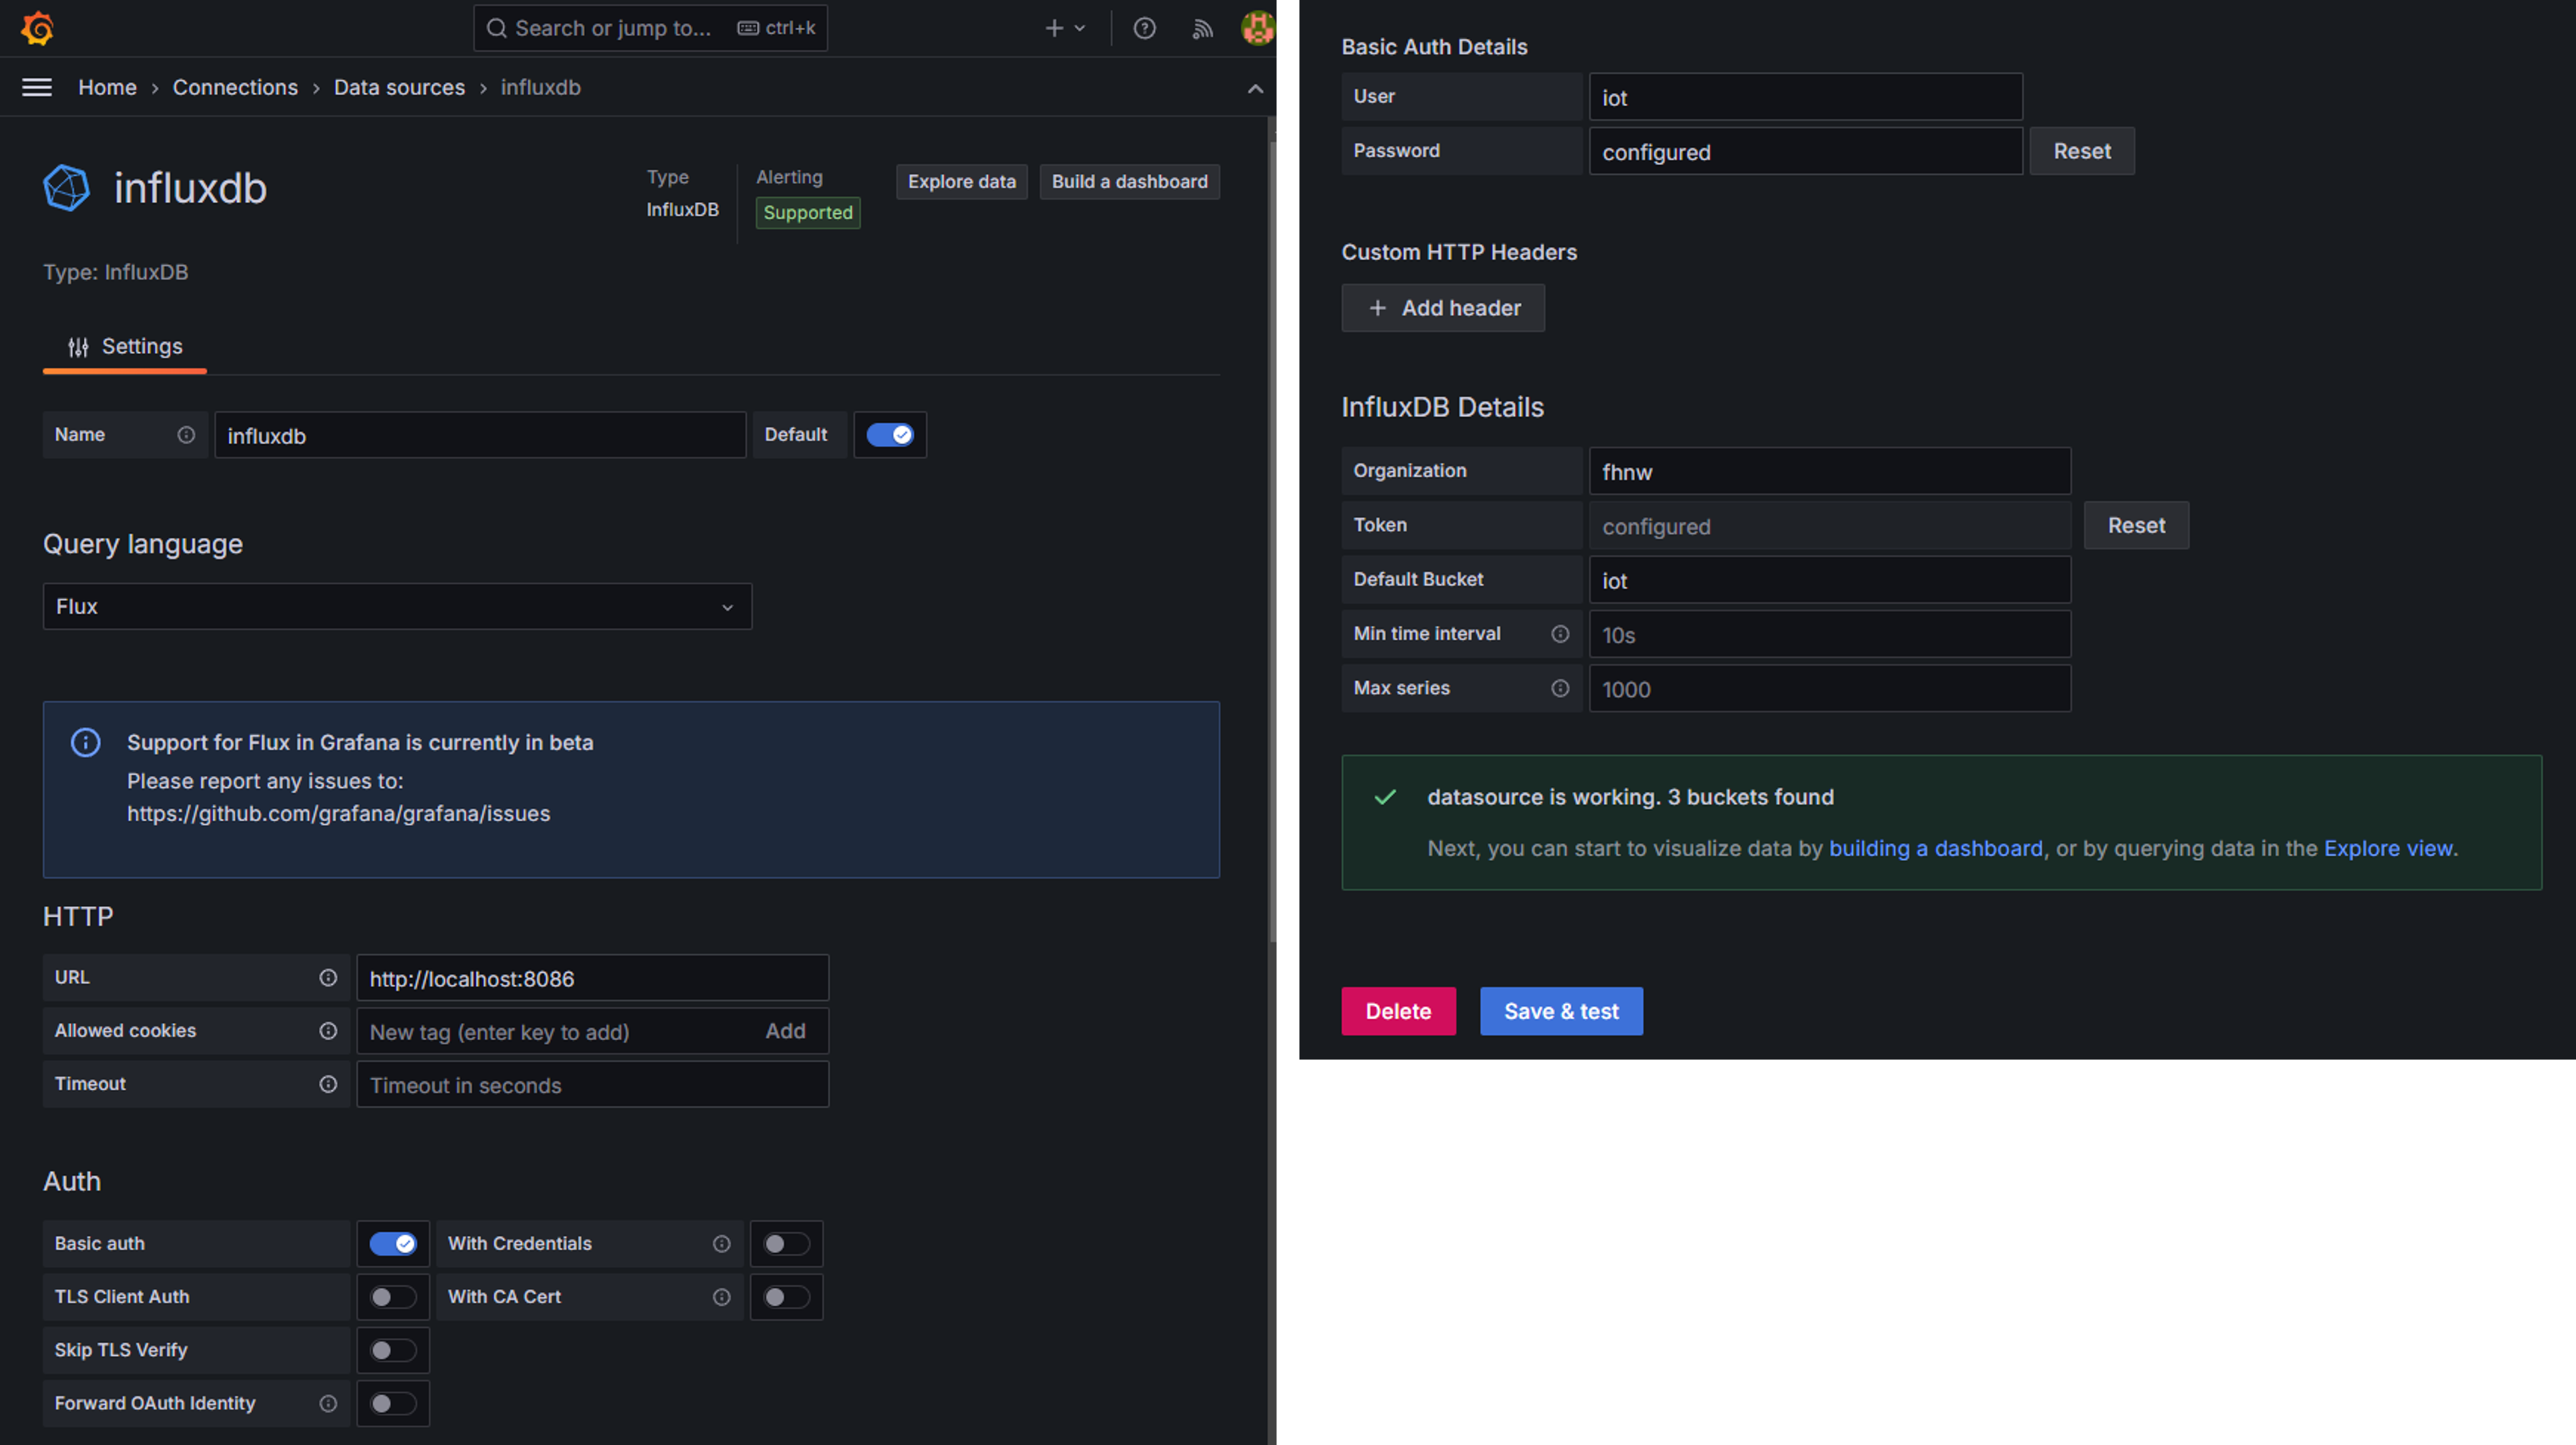
\includegraphics{images/mqtt_grafana_influxdb_settings.png}

}

\caption{\label{fig-grafanainfluxdb}InfluxDB als Datenquelle in Grafana
hinzufügen mit den entsprechenden Angaben.}

\end{figure}%

Ist die Verbindung erstellt, können neue Dashboards erstellt werden. Die
Queries, die für die Visualisierung verwendet werden sollen, können über
den \emph{Query Builder} in InfluxDB erstellt und in Grafana beim
Erstellen der Panels (Abbildung~\ref{fig-grafanainfluxdbquery})
reinkopiert werden.

\begin{figure}

\centering{

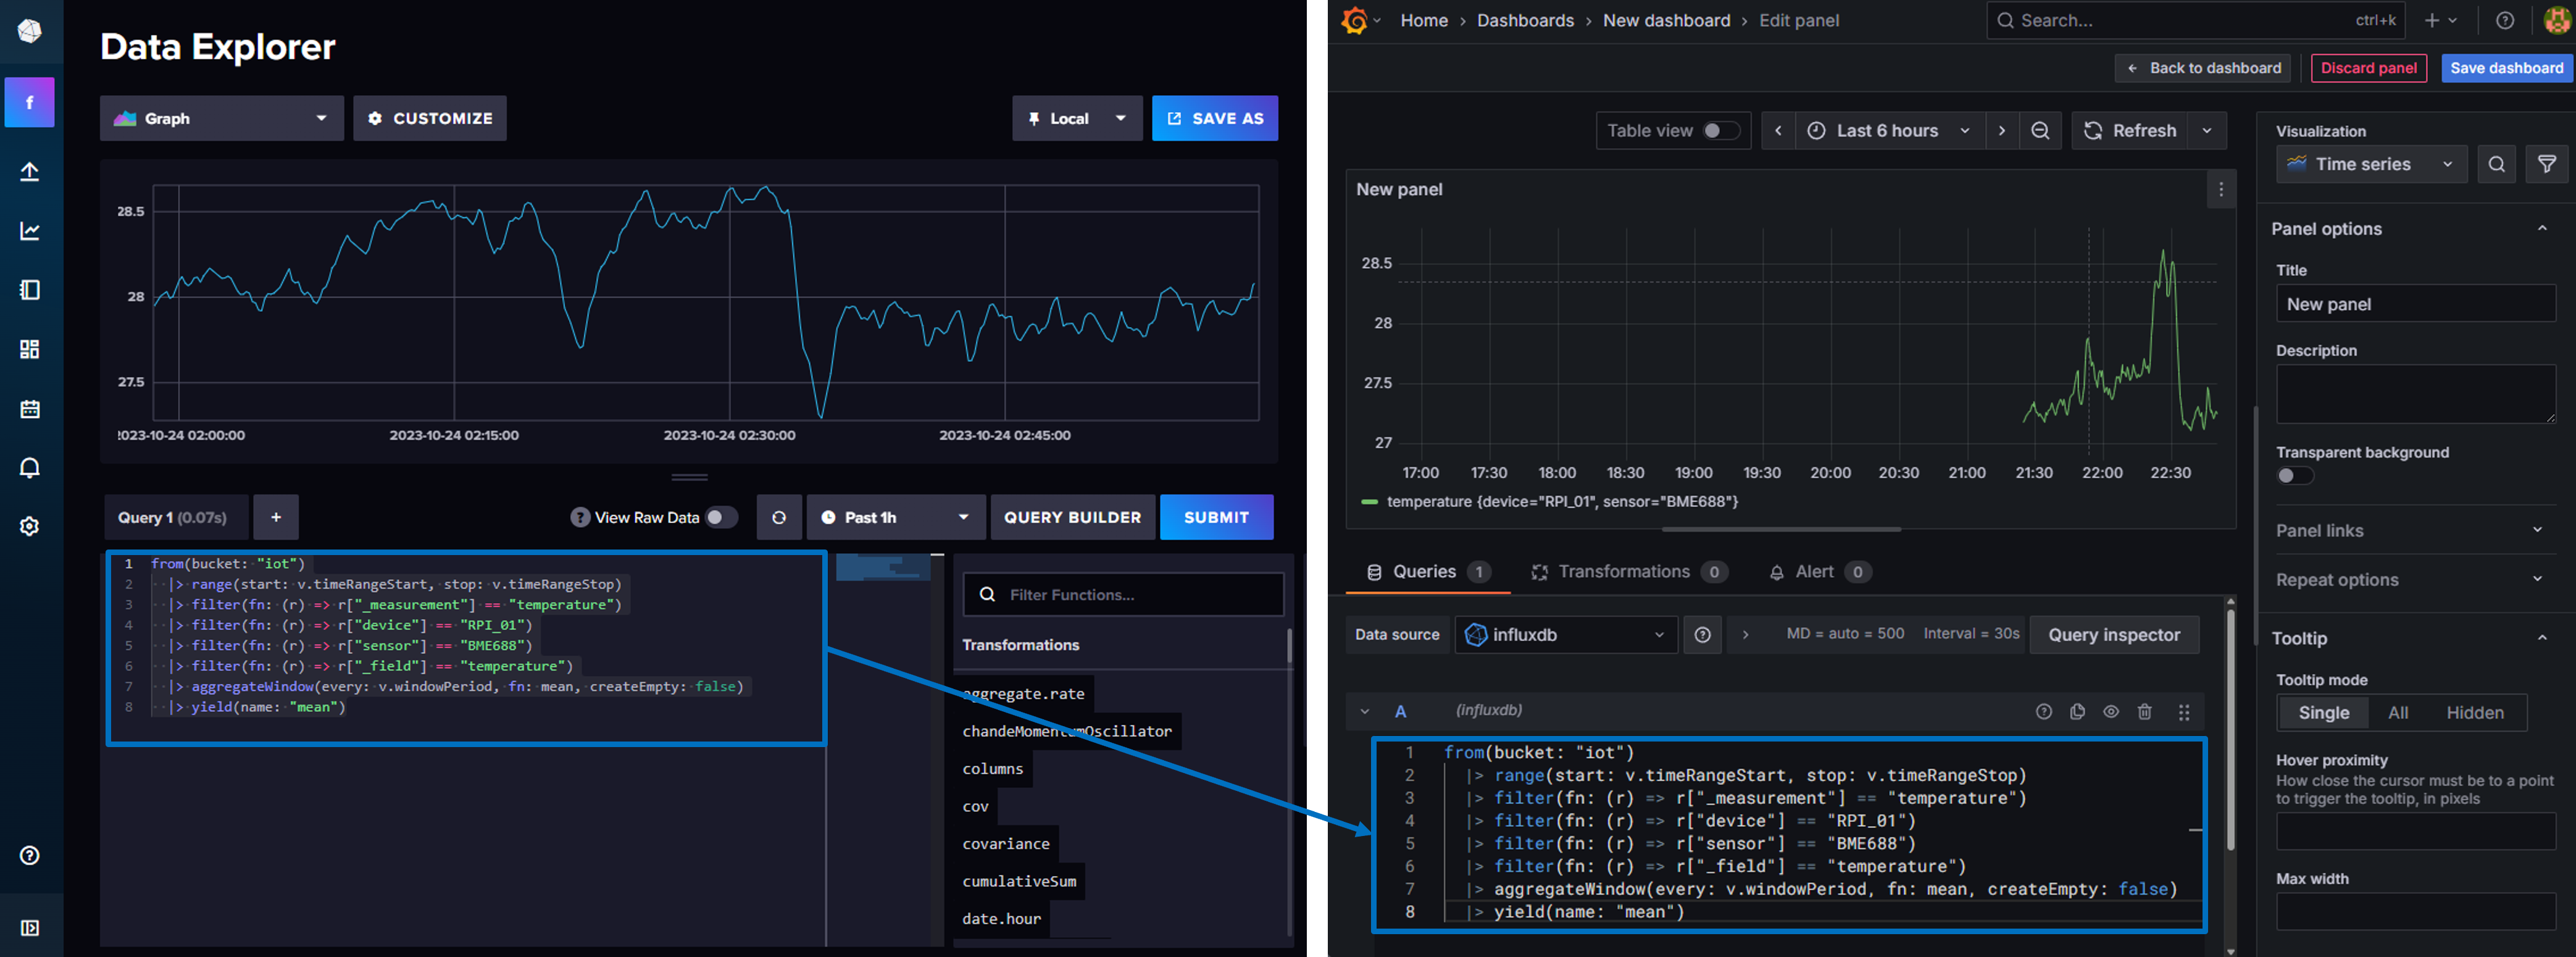
\includegraphics{images/mqtt_grafana_influxdb_query.png}

}

\caption{\label{fig-grafanainfluxdbquery}Flux Queries der Datenabfragen
im Data Explorer können in Grafana für die Visualisierung kopiert und
genutzt werden.}

\end{figure}%

\begin{boxtitle}{Excercise}{colPrimary}

\begin{itemize}
\tightlist
\item
  Erstellt eine Verbindung zwischen Grafana und der InfluxDB.
\item
  Erstellt ein Dashboard mit einer Visualisierung der Temperatur,
  Luftfeuchtigkeit und Luftdruck des BME688 Sensors.
\end{itemize}

\end{boxtitle}

\section*{Aufgabe 7: InfluxDB mit Python verwenden
(optional)}\label{aufgabe-7-influxdb-mit-python-verwenden-optional}
\addcontentsline{toc}{section}{Aufgabe 7: InfluxDB mit Python verwenden
(optional)}

\markright{Aufgabe 7: InfluxDB mit Python verwenden (optional)}

Anstatt mit Node-Red können die Daten des Sensors direkt in die InfluxDB
geschrieben werden. Folgender Code zeigt wie die Daten des BME688
Sensors mit Python ausgelesen und in die InfluxDB geschrieben werden
können. Teste erst, ob der \texttt{influxdb-client} installiert ist und
installiere diesen falls nicht mit dem Befehl
\texttt{pip3\ install\ influxdb-client}. Folgendes Tutorial zeigt wie
die Daten mit Python in die InfluxDB geschrieben werden können:
\href{https://www.influxdata.com/blog/getting-started-with-python-and-influxdb-v2-0/}{Getting
Started with Python and InfluxDB v2.0}.


\includegraphics{images/mqtt-sensor-influxdb.jpg}

\begin{Shaded}
\begin{Highlighting}[]
\ImportTok{from}\NormalTok{ datetime }\ImportTok{import}\NormalTok{ datetime}
\ImportTok{import}\NormalTok{ time}

\ImportTok{from}\NormalTok{ influxdb\_client }\ImportTok{import}\NormalTok{ InfluxDBClient, Point, WritePrecision}
\ImportTok{from}\NormalTok{ influxdb\_client.client.write\_api }\ImportTok{import}\NormalTok{ SYNCHRONOUS}

\CommentTok{\# Generieren ein Token in der InfluxDB UI unter dem Tab "Data / Tokens Tab"}
\NormalTok{token }\OperatorTok{=} \StringTok{"\textless{}influxdb{-}token\textgreater{}"}
\NormalTok{org }\OperatorTok{=} \StringTok{"fhnw"}
\NormalTok{bucket }\OperatorTok{=} \StringTok{"iot"}

\NormalTok{client }\OperatorTok{=}\NormalTok{ InfluxDBClient(url}\OperatorTok{=}\StringTok{"http://localhost:8086"}\NormalTok{, token}\OperatorTok{=}\NormalTok{ token, org}\OperatorTok{=}\NormalTok{ org)}
\NormalTok{write\_api }\OperatorTok{=}\NormalTok{ client.write\_api(write\_options }\OperatorTok{=}\NormalTok{ SYNCHRONOUS)}

\NormalTok{temperature }\OperatorTok{=} \FloatTok{22.0}
\NormalTok{data }\OperatorTok{=}\NormalTok{ Point(}\StringTok{"measures"}\NormalTok{).tag(}\StringTok{"fields"}\NormalTok{, }\DecValTok{2}\NormalTok{).field(}\StringTok{"temperature"}\NormalTok{, temperature)}
\NormalTok{write\_api.write(bucket }\OperatorTok{=}\NormalTok{ bucket, record }\OperatorTok{=}\NormalTok{ data)}
\end{Highlighting}
\end{Shaded}

\begin{boxtitle}{Excercise}{colPrimary}

Schreibe nun mit Hilfe des Tutorials und dem Beispielcode ein Python
Script, welches die Temperatur, Luftfeuchtigkeit und Luftdruck des
BME688 Sensors ausliest und in die InfluxDB schreibt.

\end{boxtitle}

\cleardoublepage
\phantomsection
\addcontentsline{toc}{part}{Anhang}
\appendix

\chapter{\texorpdfstring{Raspberry
Pi\index{Raspberry Pi}}{Raspberry Pi}}\label{raspberry-pi}

Open Source Einplatinenrechner werden in Bildung und Forschung
eingesetzt und haben eine breite Anwendung in weiteren Bereichen wie
IoT. SBCs haben grosse Bedeutung in der Ingenieur- und
Informatikausbildung, da sie sich gut für Hands-on Vermittlung komplexer
Themen eignen, und verbessern technische Fähigkeiten, stärken das
Interesse und Motivation (Ariza und Baez 2022).

\begin{description}
\tightlist
\item[System on Chip SOC \index{System on Chip SOC}]
integriert die meisten Funktionen und Komponenten auf einem Chip (CPU,
RAM, GPU, Schnittstellen) ursprünglich für eingebettete (embedded)
Systeme, heute Mobile Geräte (Mobiles, Tablets), Edge Geräte (IoT) etc.
→ Grössenreduktion, verbesserte Leistung, tiefer Stromverbrauch,
kosteneffizient, jedoch lange Entwicklungszeiten und keine Modularität.
\item[Single Board Computer SBC \index{Single Board Computer SBC}]
ist ein Computer auf einer Leiterplatine mit allen erforderlichen
Komponenten und Anschlüssen wie CPU, RAM, GPU I/O Schnittstellen etc. →
Einfach zu nutzen, tiefer Stromverbrauch, kosteneffizient, getestete
Hardware, tendenziell günstig, jedoch schwierig Anpassungen vorzunehmen,
weniger Möglichkeiten als «Multi Board Computer».
\end{description}

Der \href{https://www.raspberrypi.com}{Raspberry Pi} ist ein
preisgünstiger Einplatinencomputer (Single Board Computer SBC) in
Kreditkartenformat zum Experimentieren und Erlernen des Programmierens.
Die Motivation für die Entwicklung des Raspberry Pi war die sinkende
Anzahl Informatikstudierender an der Universität Cambridge und der
Rückgang der Informatikkenntnisse der Studierenden. Der Raspberry Pi
wird von der britischen \href{https://www.raspberrypi.org}{Raspberry Pi
Foundation} entwickelt seit 2009 entwickelt.

Url: \url{https://www.raspberrypi.com}

Raspberry Pi Modelle im Überblick:

\begin{itemize}
\tightlist
\item
  Raspberry Pi 5 (mit 4/8GB RAM ab November 2023)
\item
  Raspberry Pi 4 Model B (mit 1/2/4/8GB RAM)
\item
  Raspberry Pi 3 Model B+
\item
  Raspberry Pi 2 Zero günstige und kompakte Version (mit/ohne Bluetooth
  und WiFi)
\item
  Raspberry Pi 400 Unit (Tastatur mit integriertem Raspberry Pi)
\item
  Raspberry Pi Pico Series flexible und kompakte Microcontroller mit dem
  RP2040 Chip
\item
  Raspberry Pi Compute Module 4 (CM4 mit/ohne eMMC)
\end{itemize}

\begin{figure}[H]

{\centering 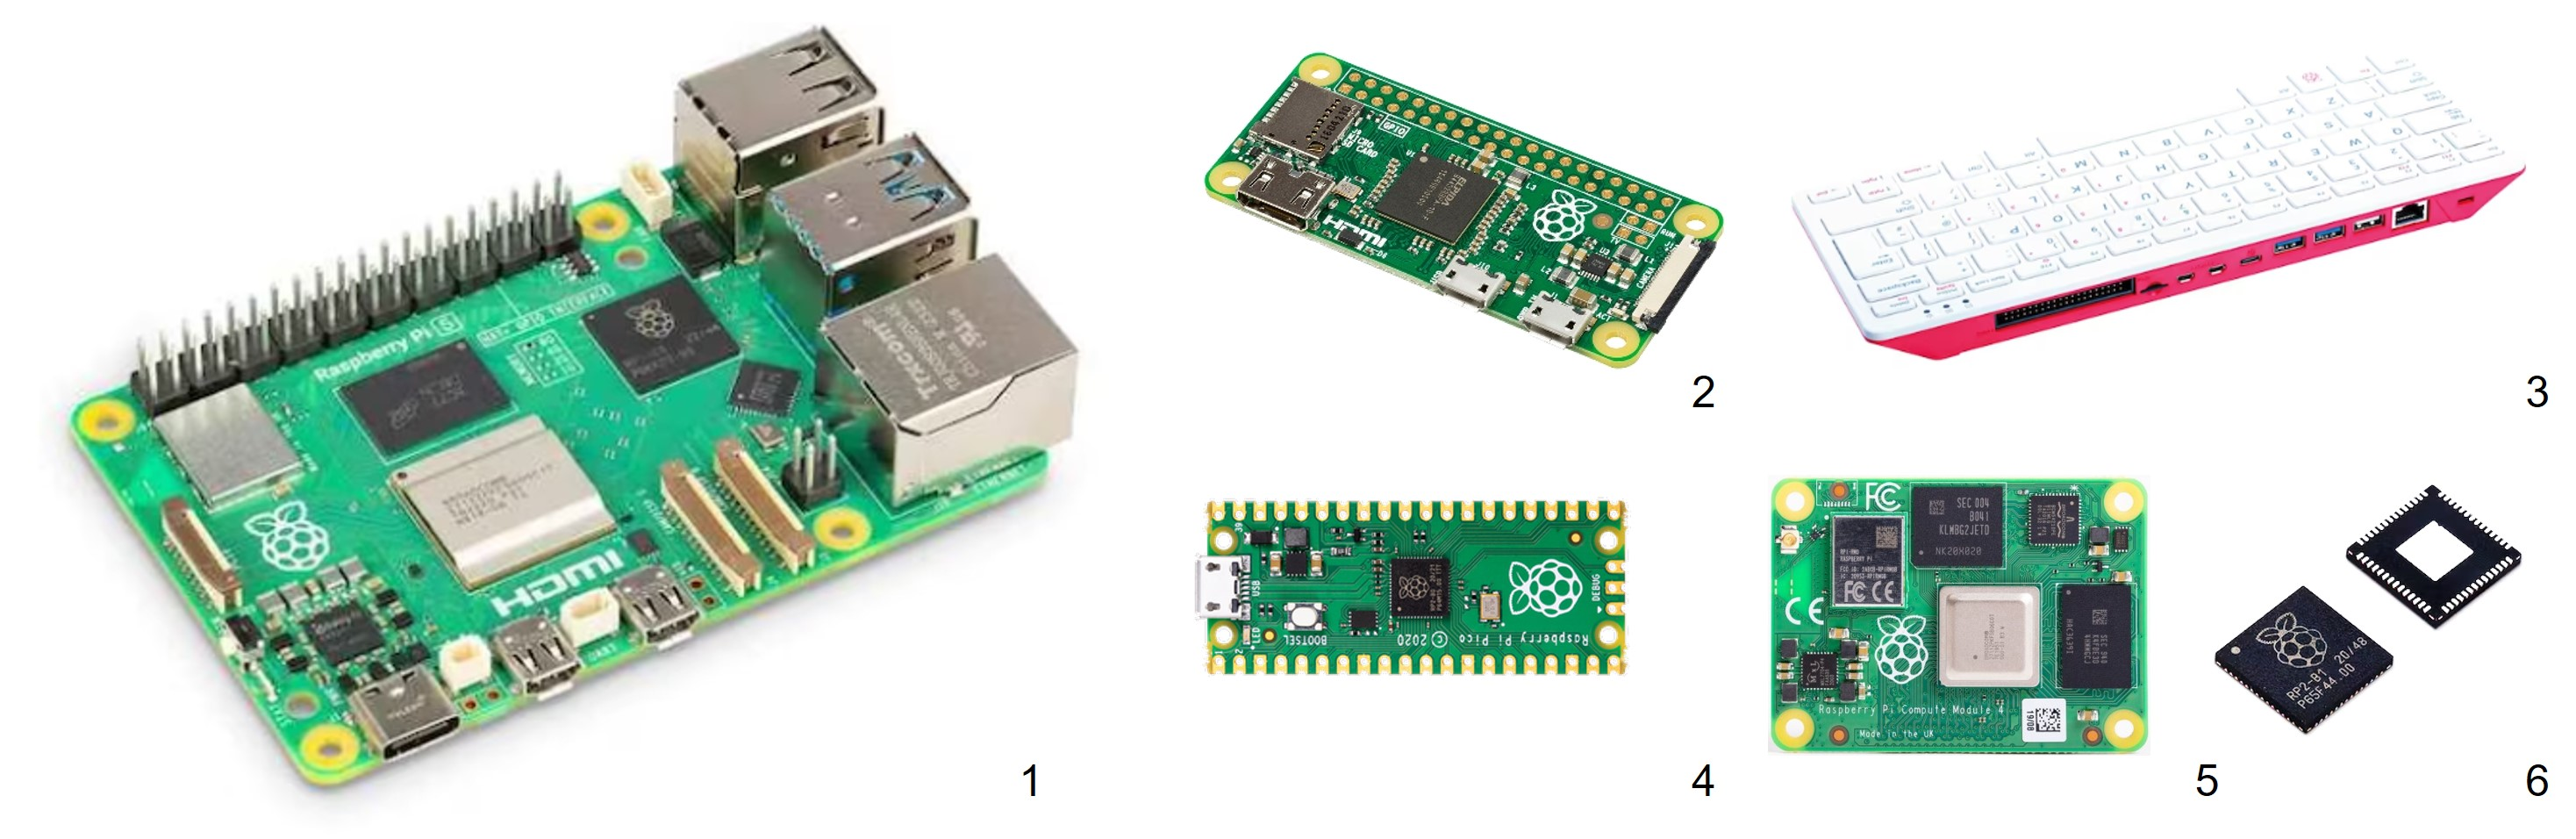
\includegraphics{images/raspberry_pi_modelle.jpg}

}

\caption{Raspberry Pi Modelle: 1. Raspberry Pi 5, 2. Raspberry Pi 2
Zero, 3. Raspberry Pi 400, 4. Raspberry Pi Pico, 5. Raspberry Pi Compute
Module 4, 6. RP2040 Chip}

\end{figure}%

Die Raspberry Pi verfügen über General Purpose Input Output
GPIO\index{General Purpose Input Output GPIO} sogenannte
Pins\index{Pins}, die für die Verbindung mit Sensoren und Aktoren
verwendet werden können. Die Stiftleiste mit den GPIO Pins sind in
unterschiedliche Gruppen unterteilt, die unterschiedliche Funktionen
haben. Die GPIO Pins können über eine Programmiersprache wie Python oder
C angesprochen werden und ermöglichen die Interaktion mit Sensoren oder
Aktoren und weiteren Komponenten.

\begin{figure}[H]

{\centering 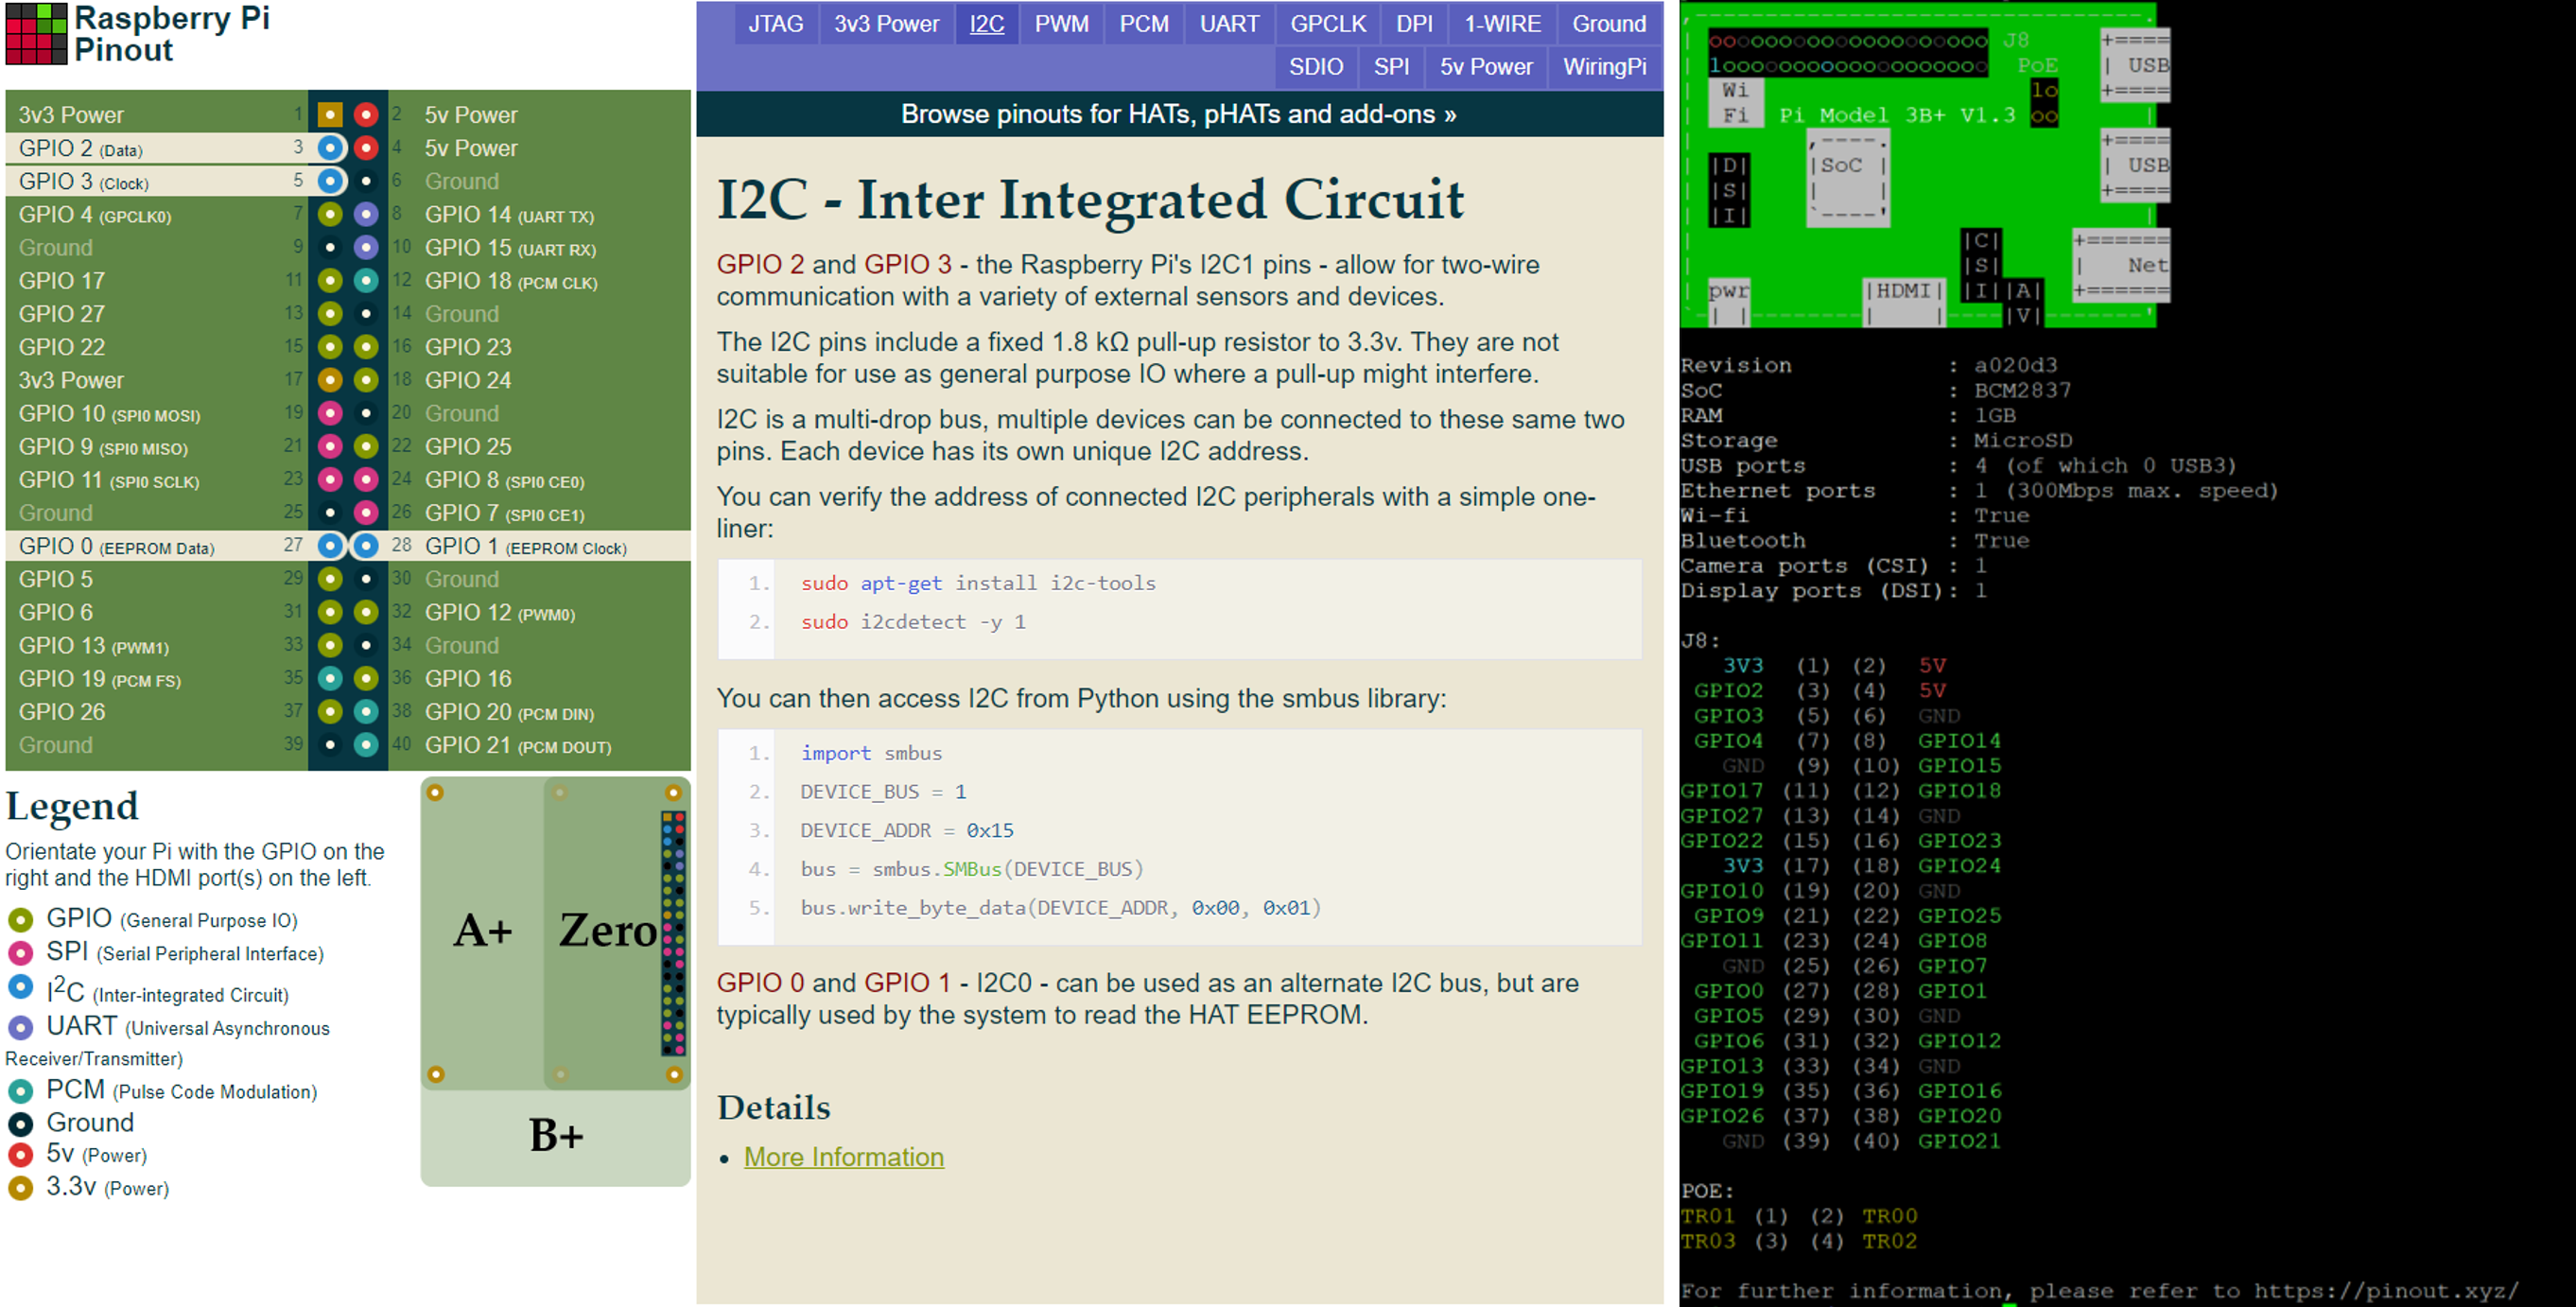
\includegraphics{images/pinout.png}

}

\caption{links: Die Website \url{https://.pinout.xyz} bietet eine
interaktive Übersicht und Dokumentation der Pinouts der einzelnen
Raspberry Pi Modellen, wie beispielsweise welche Pins die Schnittstelle
I2C ansteuern. rechts: Der Befehl \texttt{pinout} liefert direkt über
das Terminal das Pinout des Raspberry Pi}

\end{figure}%

Raspberry Pi war von der weltweiten Chip- und Halbleiterknappheit
betroffen und hatte seit 2020 tiefe Lagerbestände von elektronischen
Komponenten. Die Nachfrage nach Raspberry Pi ist seit 2020 stark
gestiegen und die Produktionskapazitäten konnten nicht erhöht werden.
Die Produktionsengpässe werden sich voraussichtlich ab Ende 2023
verbessern (Upton 2022). Die Knappheit führte zu einem Preisanstieg von
50\% bis 100\% bei den Raspberry Pi Modellen und zu einer Verknappung
der Raspberry Pi Modelle. Der Dienst
\href{https://rpilocator.com/?country=CH}{Raspberry Pi Stock Scraper}
führt eine Übersicht der Verfügbarkeit der weltweiten Raspberry Pi
Lagerbeständen von online Shops. Der
\href{https://www.pi-shop.ch/bundles-kits}{Pi-Shop} hat teilweise Kits
und Boards in der Schweiz an Lager.

\section{Raspberry Pi Image
schreiben}\label{raspberry-pi-image-schreiben}

Der Raspberry Pi führt keinen internen Speicher mit sich, sondern
benötigt eine SD-Karte. Auf dieser SD-Karte wird das Betriebssystem
installiert, respektive als Image auf die MicroSD Karte geschrieben. Die
SD-Karte muss mindestens 8 GB Speicherplatz haben idealerweise 16 GB
oder mehr.

Software: \href{https://www.raspberrypi.com/software}{Raspberry Pi -
Software}\\
Tutorial:
\href{https://www.raspberrypi.com/tutorials/how-to-set-up-raspberry-pi}{Raspberry
Pi - How to set up Raspberry Pi}

\textbf{Raspberry Pi Imager}\index{Raspberry Pi Imager} ist die von
Raspberry Pi erstellte Software für das Schreiben von Images auf eine SD
Karte. Der Imager stellt direkt auch weitere Images wie Ubuntu,
Medienzentren, 3D Druck etc. zur Verfügung. Alternative \emph{Image
Burner} sind \href{https://www.balena.io/etcher}{Balena Etcher} und
\href{https://sourceforge.net/projects/win32diskimager/}{Win32DiskImager}.

Das Betriebssystem \textbf{Raspberry Pi OS}\index{Raspberry Pi OS} ist
ein auf Debian basiertes Betriebssystem mit Anpassungen für die Hardware
auf dem Raspberry Pi. Es gibt eine \textbf{Lite} Version ohne Desktop
und eine \textbf{Desktop} Version mit Desktop. Die \textbf{Desktop}
Version ist für den Einstieg empfehlenswert, da sie die grafische
Oberfläche bietet und die Konsole. Die \textbf{Lite} Version ist für den
produktiven Einsatz empfehlenswert, da sie weniger Ressourcen benötigt
und somit mehr Ressourcen für die Anwendungen zur Verfügung stehen. Dazu
muss der Raspberry Pi über das Netzwerk erreichbar sein, beispielsweise
über SSH.

\begin{boxtitle}{Hinweis}{colPrimary}

Für die Nutzung am Campus nutzen wir die \textbf{Desktop} Version, da
wir die grafische Oberfläche für das aktivieren des Internetzugangs
benötigen.

\end{boxtitle}

Image schreiben mit \textbf{Raspberry Pi 64-bit} (Desktop Version) und
mit den erweiterten Optionen Voreinstellungen zu \textbf{SSH} (Ja),
\textbf{WiFi} (Heimnetzwerk), \textbf{Konto} und unter Sprache die
\textbf{Zeitzone} Europe/Zurich und das das \textbf{Tastaturlayout} CH
setzen.

\begin{boxtitle}{Hinweis}{colPrimary}

Die Einstellungen können später in der Konsole mit dem Programm
\texttt{raspi-config} geändert werden.

\end{boxtitle}

\begin{figure}[H]

{\centering 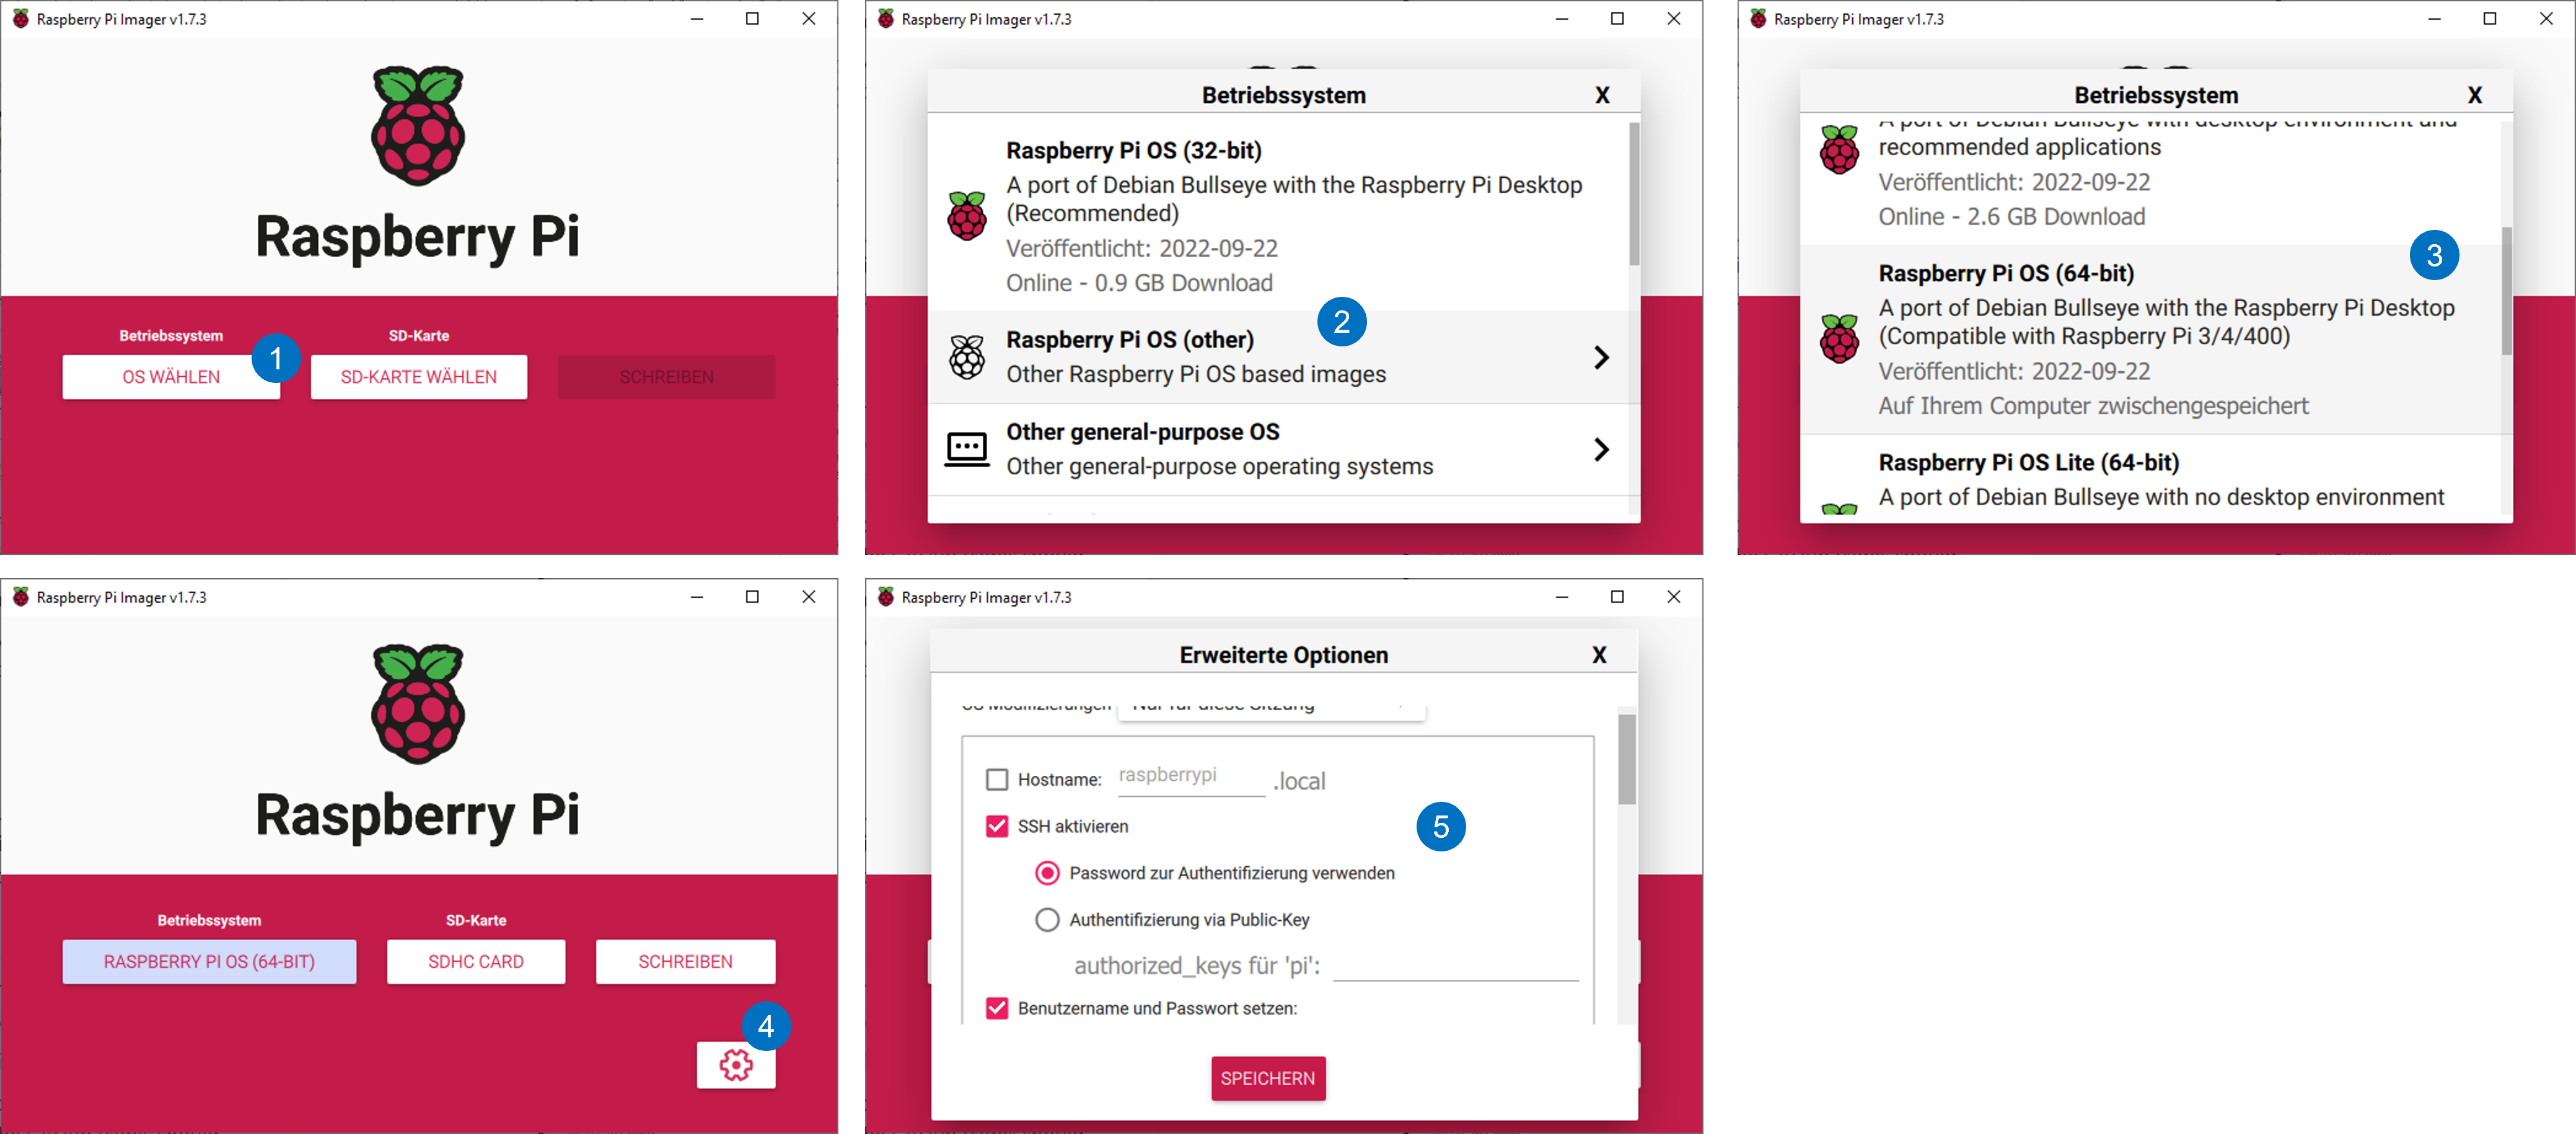
\includegraphics{images/raspberry_pi_image_schreiben.png}

}

\caption{Rasperry Pi Imager ausführen mit (1) Betriebssystem wählen, (2)
Raspberry Pi OS (Other), (3) Raspberry Pi OS 64-bit, (4) erweiterte
Einstellungen wählen und unter diesen Voreinstellungen zum Konto, SSH,
Zeitzone und Tastaturlayout vordefinieren.}

\end{figure}%

\begin{boxtitle}{Hinweis}{colPrimary}

Für Testzwecke kann es sinnvoll sein den Standardkontonamen \texttt{pi}
und das Standardpasswort \texttt{raspberry} zu verwenden. Jedoch sollte
der Kontonamen und das Passwort für den produktiven Einsatz geändert
werden, vor allem wenn der Raspberry Pi mit dem Internet verbunden ist,
beispielsweise mit einem aktivierten SSH Zugang.

\end{boxtitle}

\begin{boxtitle}{Excercise}{colPrimary}

\textbf{Raspberry Pi Image auf SD-Karte schreiben}

\begin{enumerate}
\def\labelenumi{\arabic{enumi}.}
\tightlist
\item
  Installiere den Raspberry Pi Imager
\item
  Schreibe Raspberry Pi OS 64-bit auf die SD Karte
\item
  Aktiviere SSH und setze die Spracheinstellungen (WiFi Name und
  Password des Netzwerks von Zuhause oder dem Mobile Hotspot)
\item
  SD Karte in den Raspberry einsetzen
\item
  Maus, Tastatur und Monitor anschliessen und dann mit dem Netzteil mit
  Strom versehen
\end{enumerate}

\end{boxtitle}

\section{Raspberry Pi einrichten}\label{raspberry-pi-einrichten}

Für das Einrichten des Raspberry Pi wird die SD-Karte mit dem Image in
den Raspberry Pi eingesetzt. Für das erstmalige Einrichten des Raspberry
Pi OS ist ein Bildschirm, eine Tastatur und eine Maus erforderlich.
Verbunden wird der Raspberry Pi über die HDMI-Schnittstelle mit dem
Bildschirm und über die USB Schnittstelle mit der Tastatur und der Maus,
dann wird die Stromversorgung über USB-C angeschlossen.

\begin{boxshade}{colPrimary}

\textbf{Gehäuse öffnen und SD Karten Slot öffnen}

Den Deckel durch leichtes Drücken mit zwei Finger bei (1) horizontal
leicht in Pfeilrichtung drücken, nach einem Klick lässt sich das Gehäuse
aufschieben. Der SD Karten-Slot lässt sich mit einem Stift in der
Einbuchtung (3) mit leichtem Druck in Pfeilrichtung öffnen (4). Das
Raspberry Pi Board kann durch ein leichtes Klicken in Pfeilrichtung (5)
aus dem Gehäuse entfernt werden.

\begin{figure}[H]

{\centering 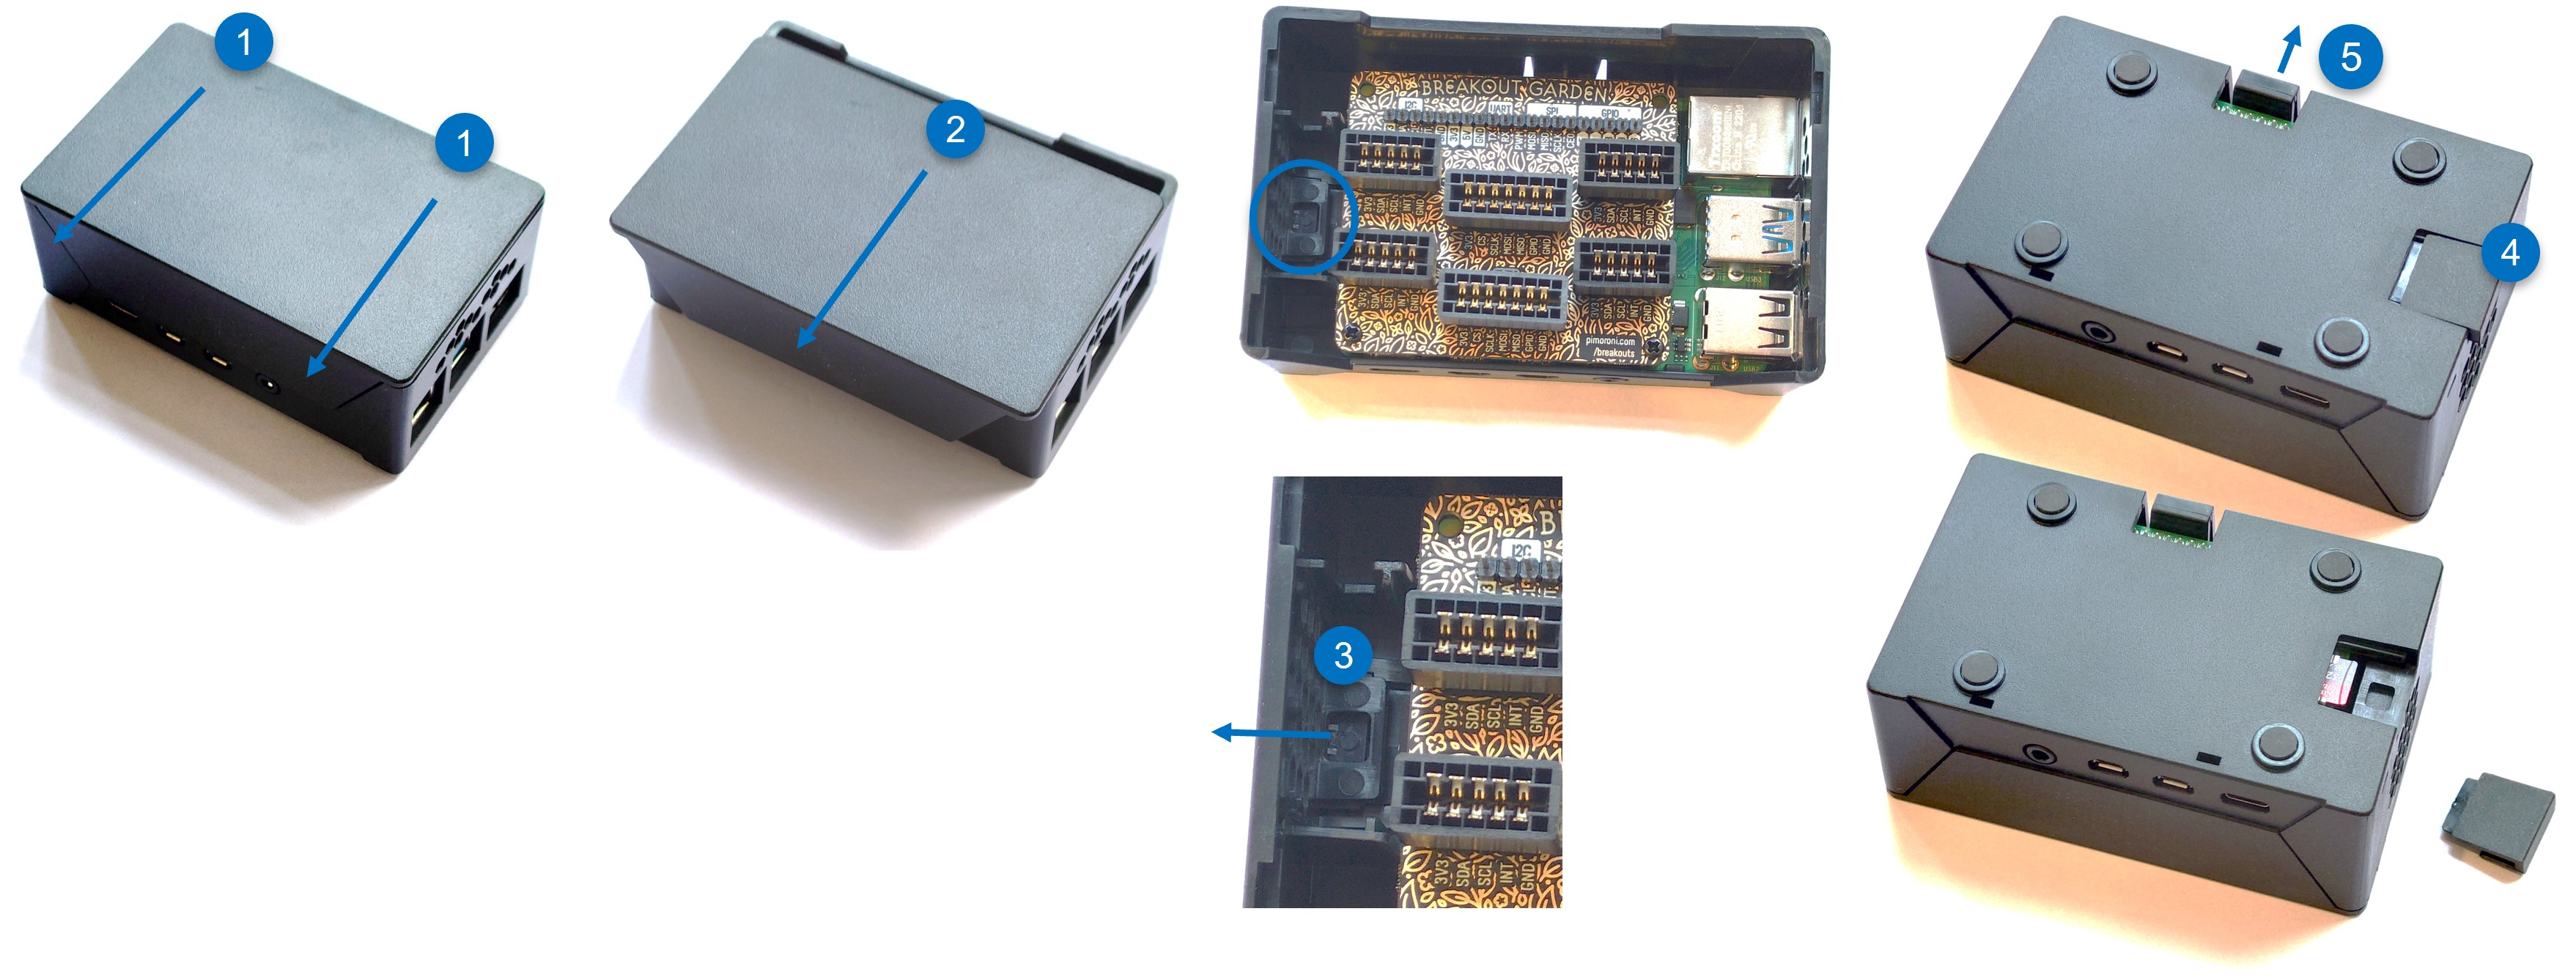
\includegraphics{images/raspberry_pi_oeffnen_sd_karte_wechseln.jpg}

}

\caption{Gehäuse öffnen, SD Karte wechesln und das Board aus dem Gehäuse
entfernen.}

\end{figure}%

\end{boxshade}

\section{WiFi Verbindung einrichten}\label{wifi-verbindung-einrichten}

Das WiFi Network kann auch über den Desktop eingerichtet werden. Das
WiFi Symbol in der oberen rechten Ecke des Desktops zeigt die
verfügbaren WiFi Netzwerke an. Je nach Einstellungen muss hierbei noch
das WiFi Land \texttt{CH} ausgewählt werden. Die WiFi Einstellungen
können auch über die Konsole mit dem Programm \texttt{raspi-config}
vorgenommen werden.

\begin{boxtitle}{Hinweis}{colPrimary}

Für die Verbindung mit dem Internet am Campus muss das Netzwerk
\emph{fhnw-public} ausgewählt werden. Im Browser kann über die Website
\url{https://mpp.ict.fhnw.ch} mit dem FHNW Login oder über das
Mobiltelefon die Verbindung hergestellt werden.

\end{boxtitle}

\begin{figure}[H]

{\centering 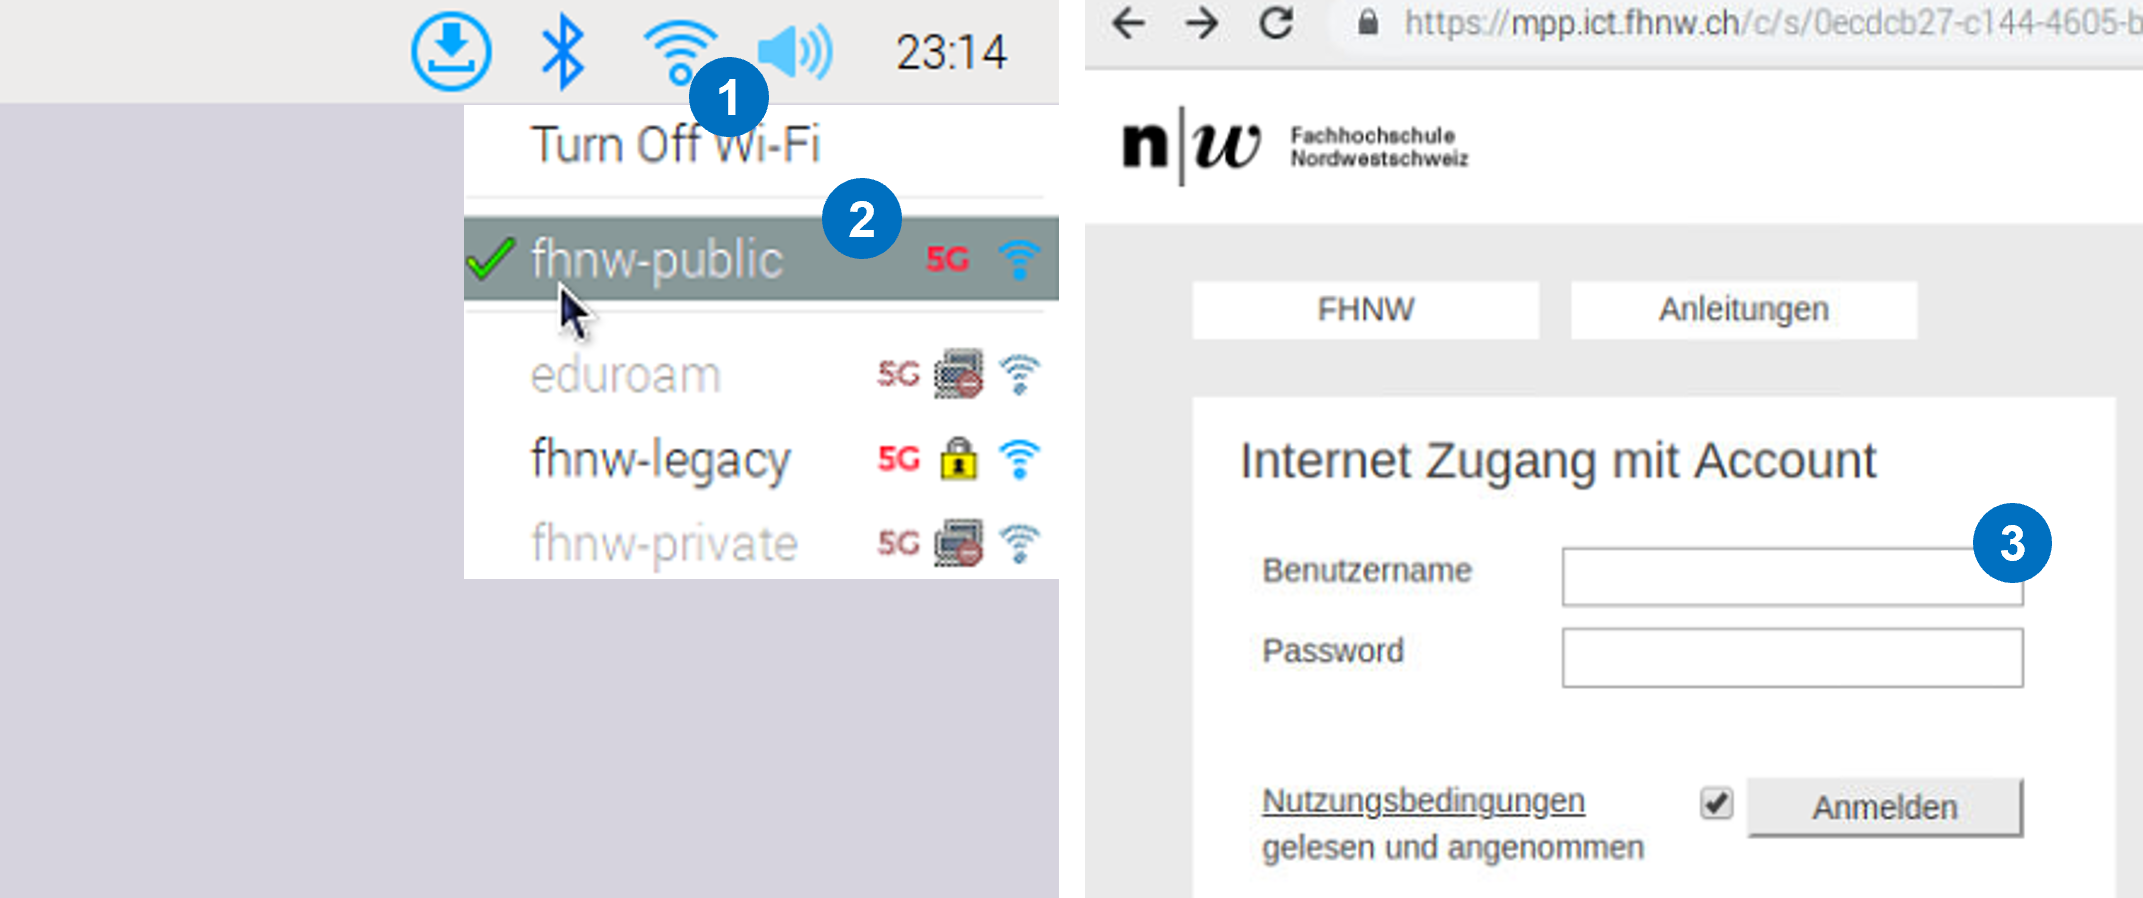
\includegraphics{images/raspberry_pi_image_wifi_cmu.png}

}

\caption{WiFi Verbindung über den Desktop auf dem Campus herstellen. Das
Netzwerk \emph{fhnw-public} wählen und auf der Website
https://mpp.ict.fhnw.ch die Verbindung mit dem FHNW Account oder via
Mobile herstellen.}

\end{figure}%

\section{\texorpdfstring{SSH Verbindung
herstellen\index{SSH}}{SSH Verbindung herstellen}}\label{ssh-verbindung-herstellen}

\begin{marginfigure}

\centering{

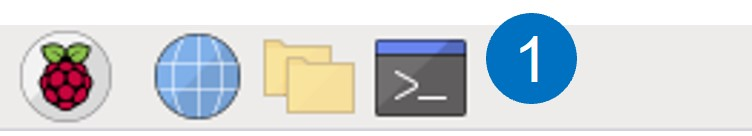
\includegraphics{images/raspberry_pi_shell.jpg}

}

\caption{\label{fig-shell}Shell über die Softwareleiste öffnen}

\end{marginfigure}%

Das SSH Protokoll ermöglicht den direkten auf den Raspberry Pi über das
Konsolenfenster. Hierfür wird die IP Adresse des Raspberry Pi benötigt.
Die IP Adresse kann über das Programm \texttt{ifconfig} oder
\texttt{ip\ addr} in der Konsole abgefragt werden.

\begin{figure}[H]

{\centering 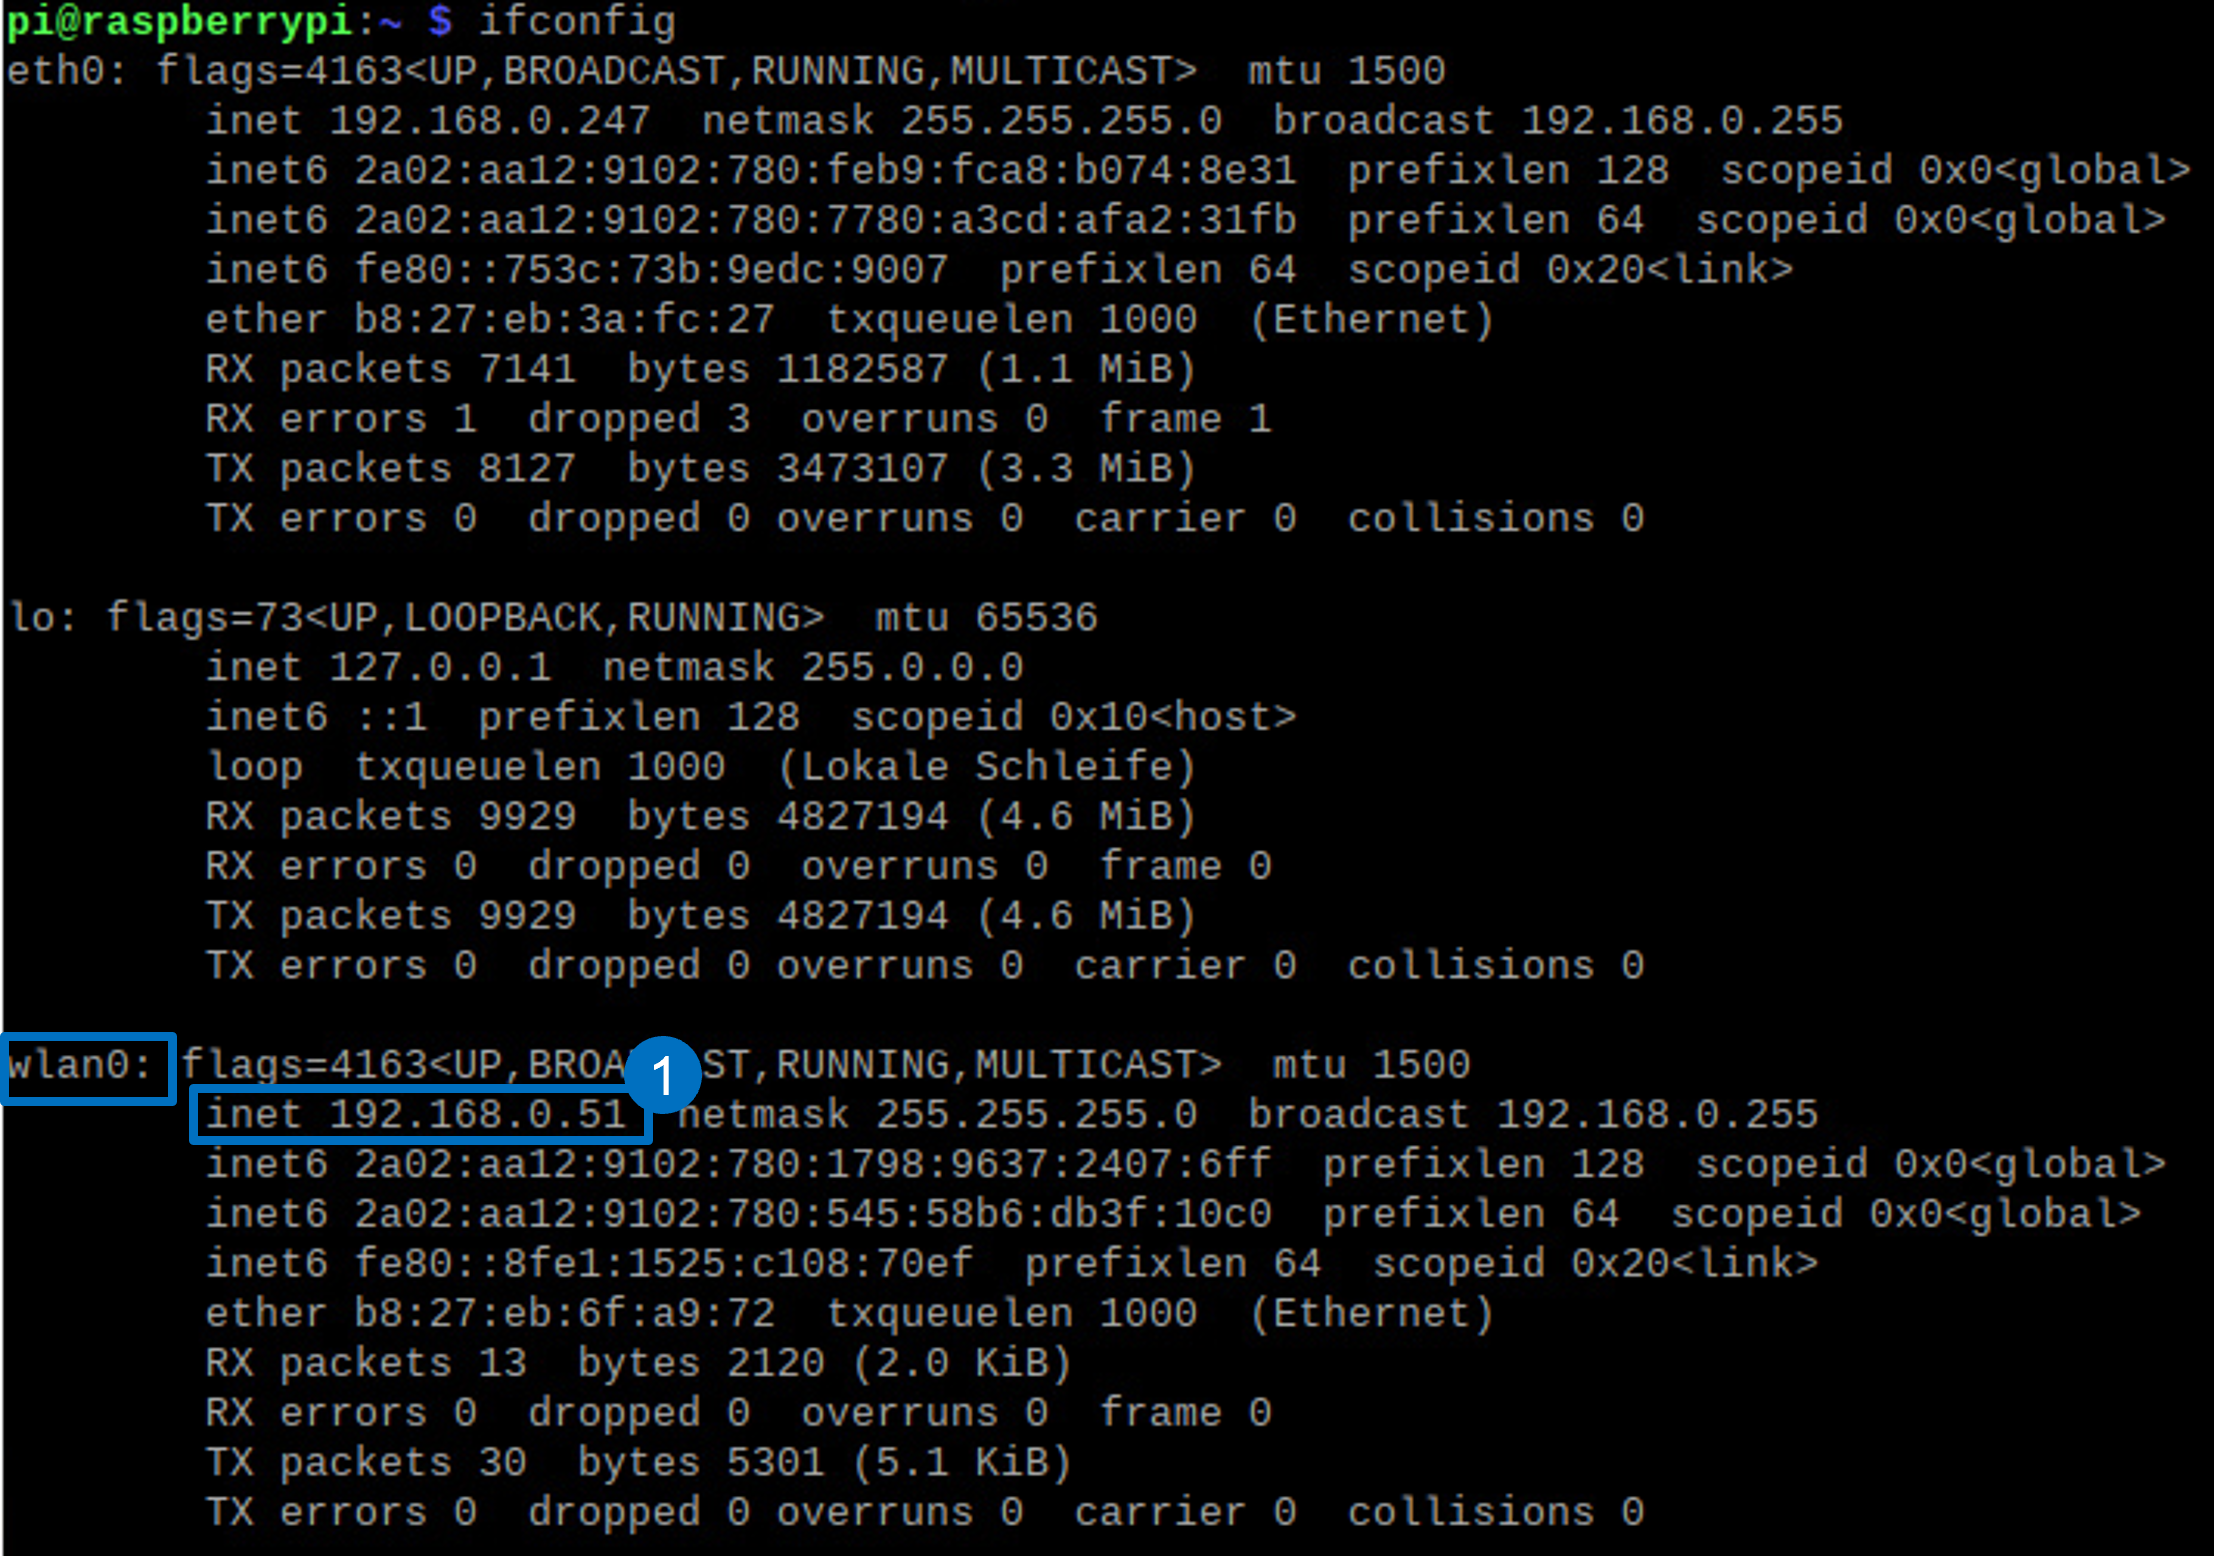
\includegraphics{images/raspberry_pi_ifconfig.png}

}

\caption{Die IP-Adresse für das Wi-Fi ist unter \texttt{wlan0} bei inet
aufgeführt. Falls der Raspberry Pi mit einem Ethernet Kabel mit dem
Netzwerk verbunden ist, wird die IP Adresse unter \texttt{eth0} bei inet
aufgeführt.}

\end{figure}%

Für die Verbindung mit SSH zu Raspberry Pi existieren unterschiedliche
Clients:

\begin{itemize}
\tightlist
\item
  Direkt über die Eingabeaufforderung in Windows mit \texttt{ssh}
\item
  PuTTY \url{https://putty.org} (win) ein SSH und telnet client für
  Windows (auch portable Nutzung ohne Installation möglich)
\item
  Tabby \url{https://tabby.sh} (win, mac, linux) ein modernes open
  source Terminal für lokale Shell, Serielle Schnittstelle, SSH und
  Telnet Verbindungen, File Transfer mit SFTP und
  Konfigurationsmöglichkeiten (auch portable Nutzung ohne Installation
  möglich)
\end{itemize}

\begin{figure}[H]

{\centering 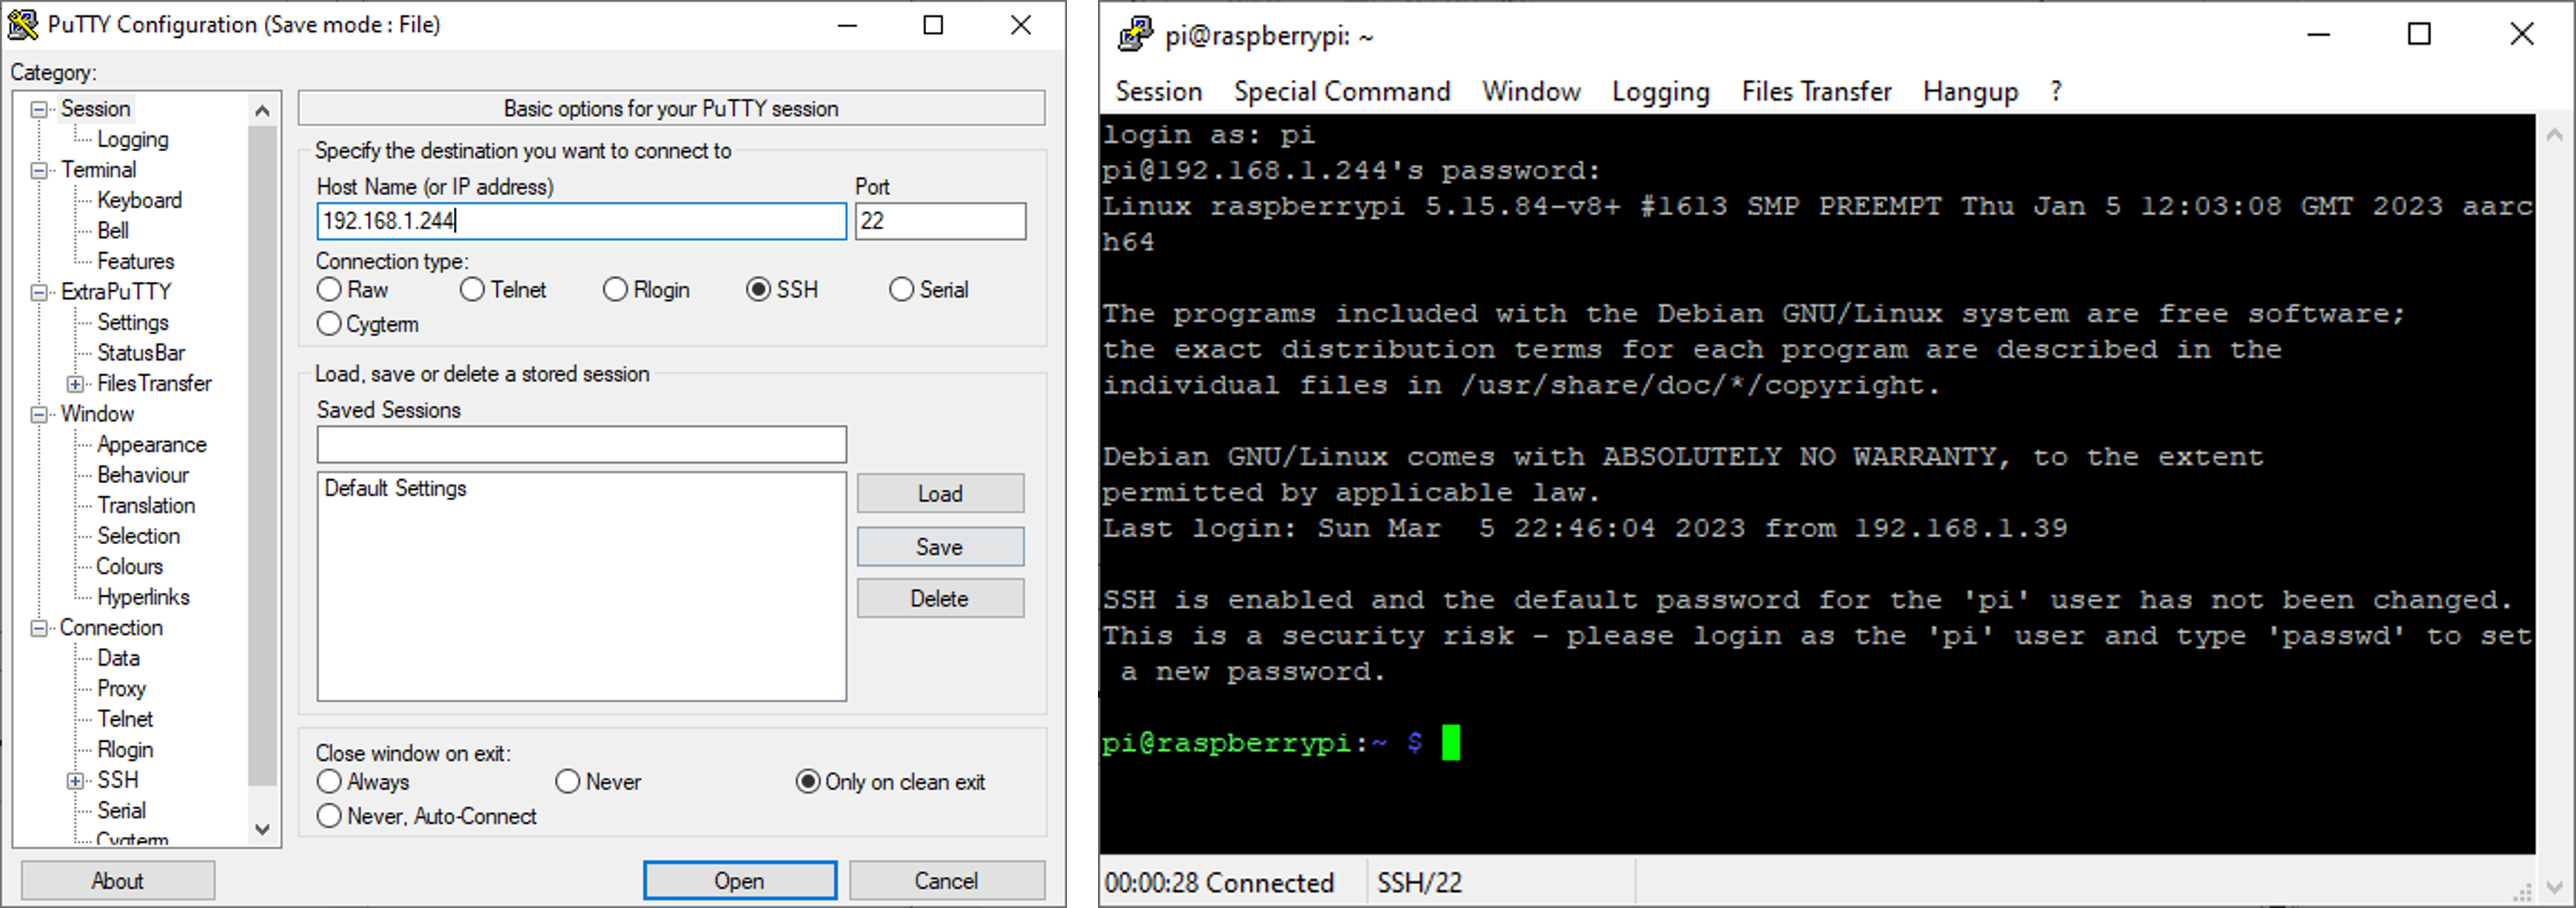
\includegraphics{images/raspberry_pi_putty.png}

}

\caption{SSH Verbindung mit Putty einrichten}

\end{figure}%

\subsection{\texorpdfstring{Tabby\index{Tabby}}{Tabby}}\label{tabby}

Neues SSH Verbindungsprofil mit Tabby erstellen mit der IP Adresse des
Raspberry Pi erstellen.

\begin{enumerate}
\def\labelenumi{\arabic{enumi}.}
\tightlist
\item
  Unter Einstellungen / Profile \& Verbindungen ein Neues Profil anlegen
\item
  In der Auswahl SSH-Verbindung wählen
\item
  Unter Host die IP Adresse Benutzername des Raspberry Pi setzen und
  speichern
\end{enumerate}

\begin{figure}[H]

{\centering 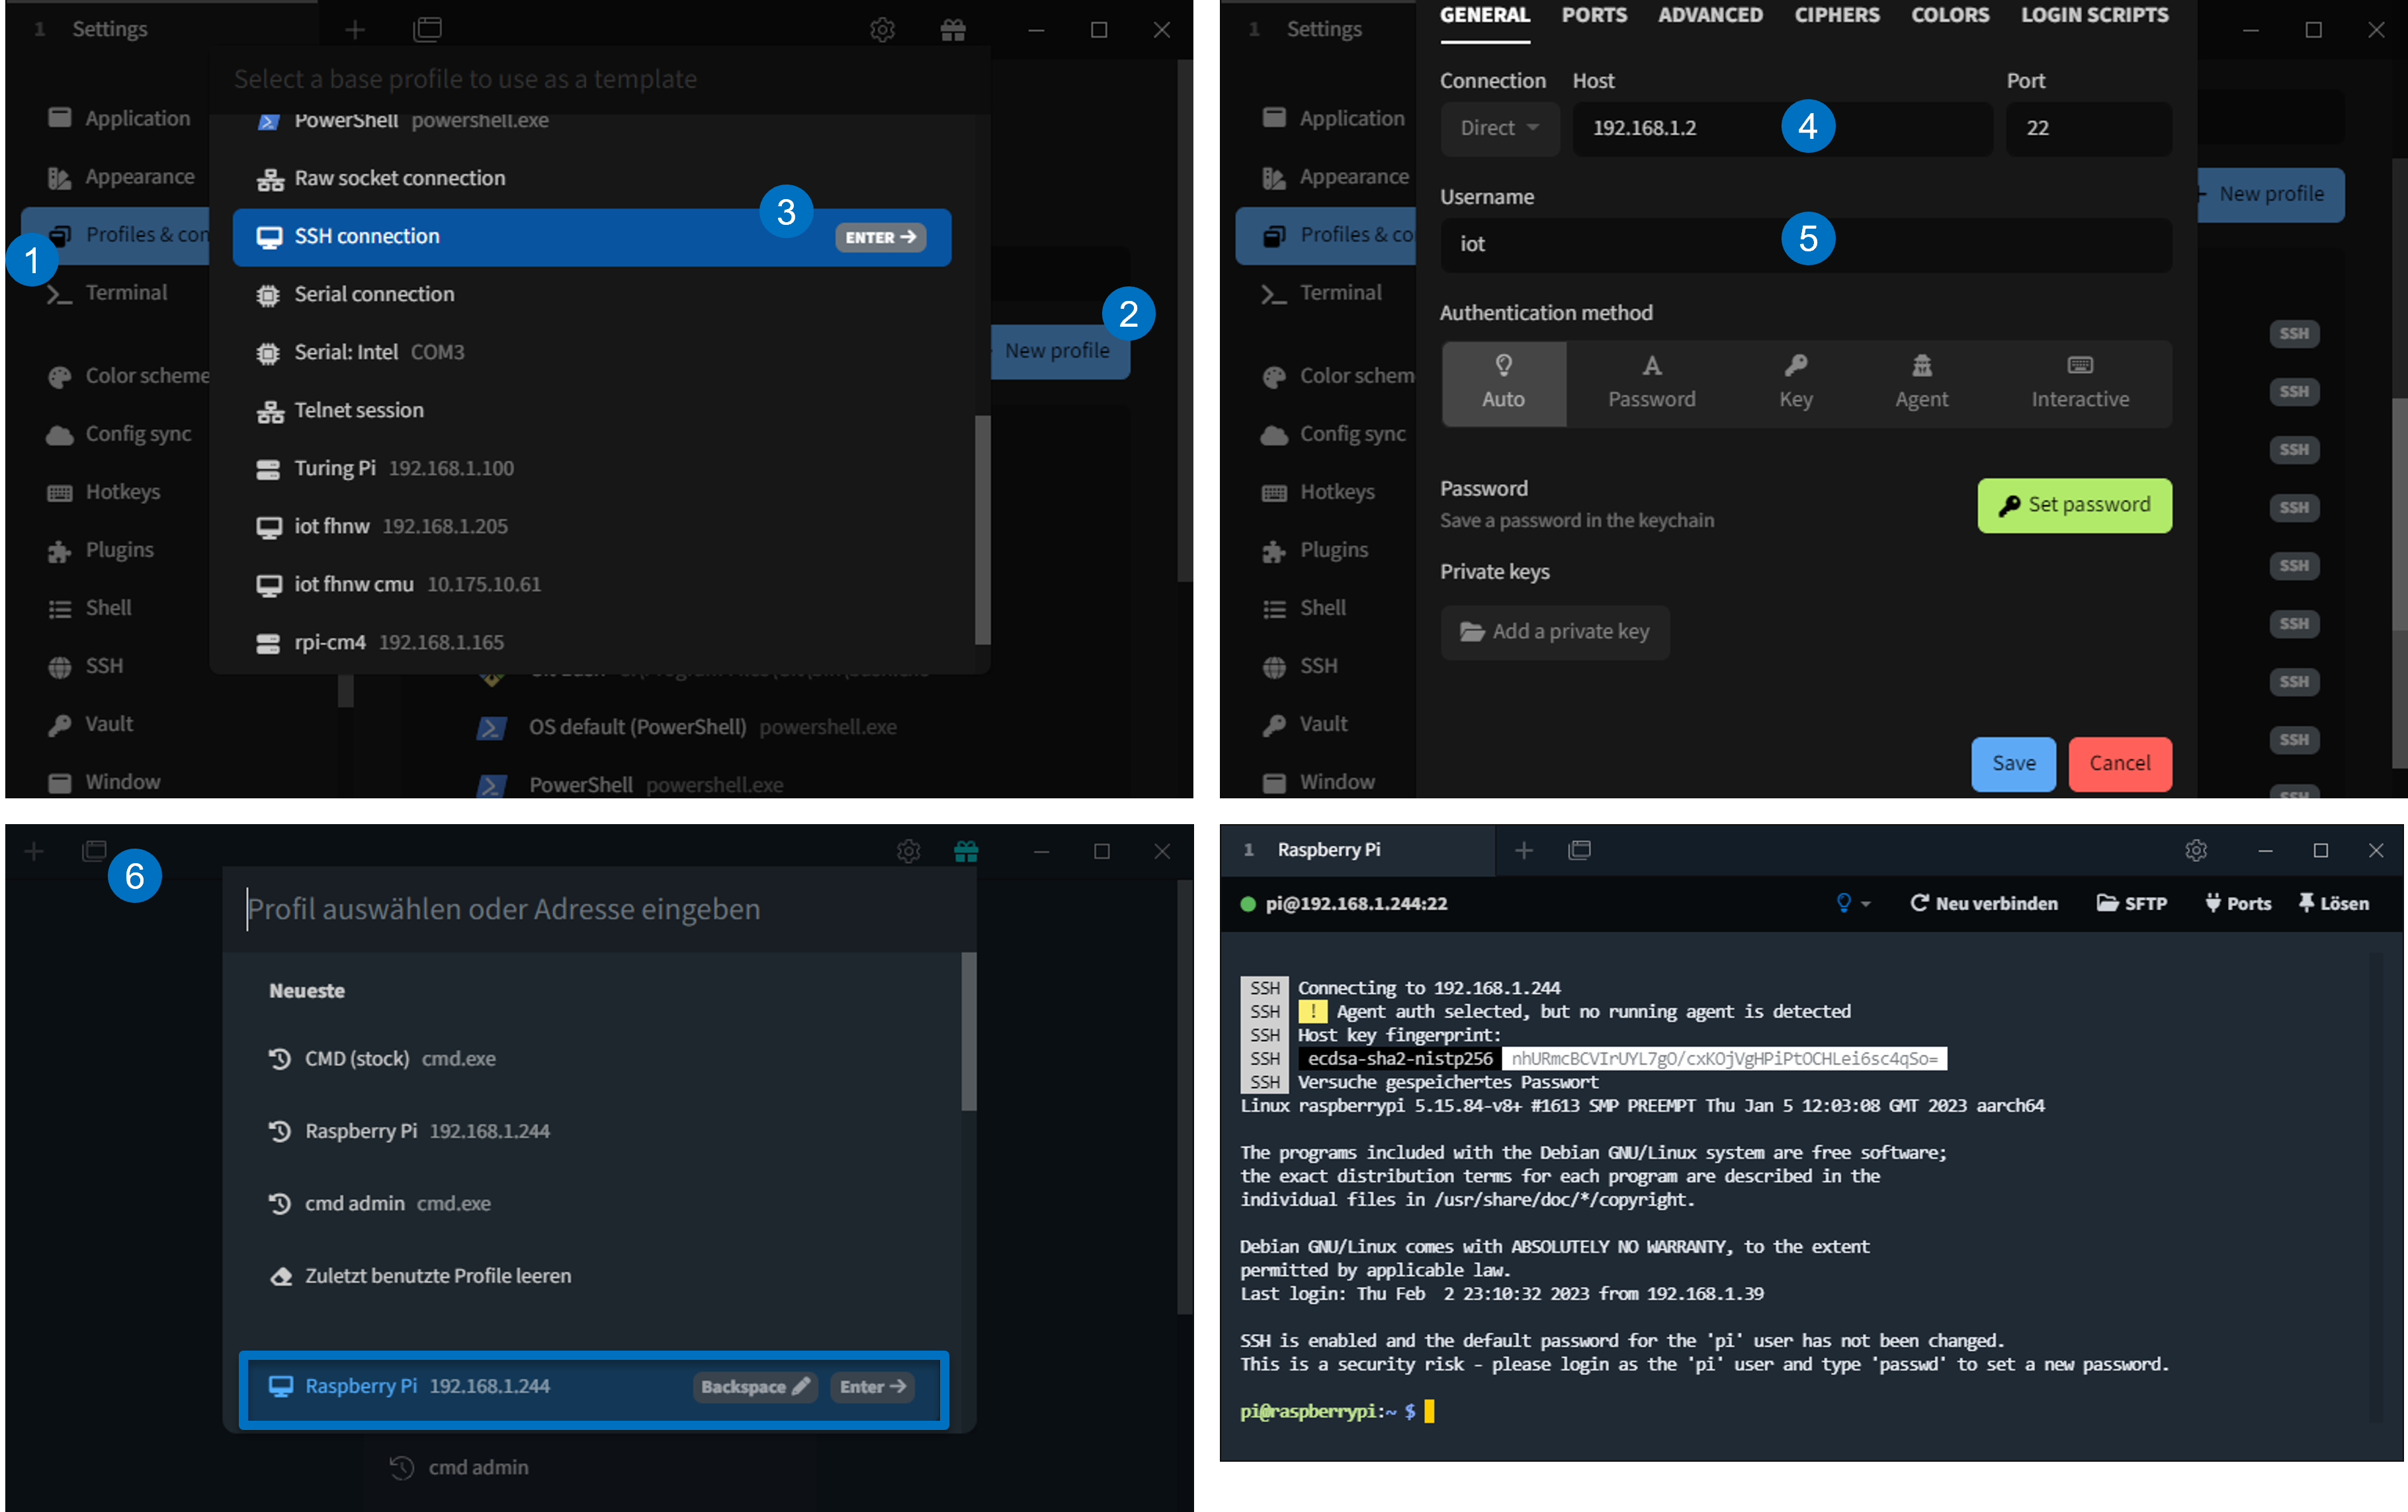
\includegraphics{images/raspberry_pi_tabby.png}

}

\caption{SSH Verbindung mit Tabby einrichten (1-5) und anwenden (6).}

\end{figure}%

\subsection{Datentransfer mit SFTP}\label{datentransfer-mit-sftp}

Remote Datentransfer mit SFTP dem SSH File Transfer
Protokoll\index{SFTP SSH File Transfer Protokoll} ermöglicht ein
einfaches Verwalten und auch sichern der Daten. Hierbei eignet sich die
Software \href{https://filezilla-project.org/}{FileZilla} oder
\href{https://winscp.net/eng/docs/lang:de}{WinSCP} für den
Datentransfer.

In Fillezilla eine SFTP Verbindung über Datei/Servermanager herstellen
mit Server:
\texttt{\textless{}IP\ Adresse\ Raspberry\ Pi\textgreater{}}, Protokoll:
\texttt{SFTP}, und bei der Verbindungart \texttt{normal} wählen und dort
Benutzername und Passwort des Raspberry Pi Users angeben.

\begin{figure}[H]

{\centering 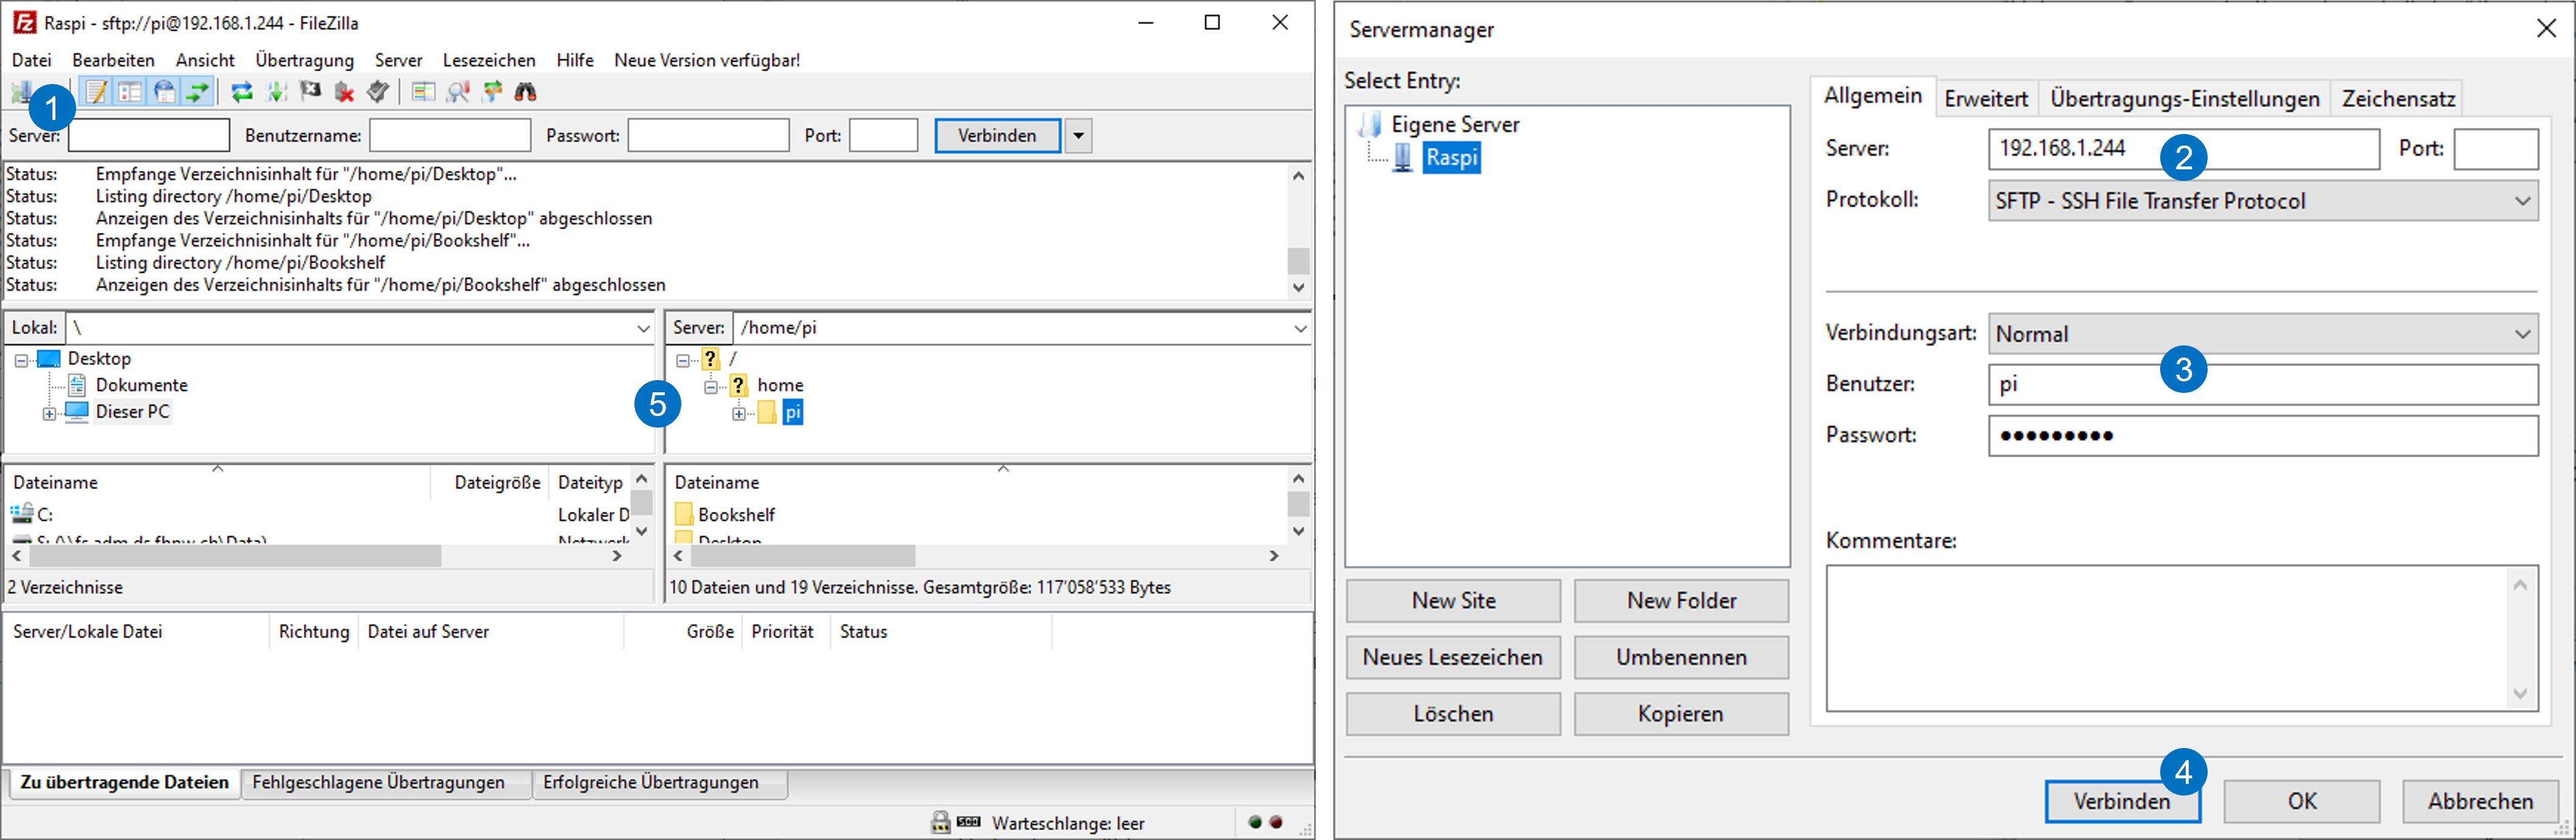
\includegraphics{images/raspberry_pi_filezilla.png}

}

\caption{Datentransfer mit FileZilla. Eine neue Verbindung im
Servermanager (1) erstellen unter Server die IP-Adresse des Raspberry Pi
setzen mit dem SFTP Prokoll, und bei der Verbindungsart \emph{normal}
wählen und Benutzername und Passwort des Raspberry Pi angeben und mit
``Verbinden'' (4) die SFTP Verbindung aufbauen und im Hauptfenster (5)
Daten transferieren.}

\end{figure}%

\section{Mobilen Hotspot nutzen}\label{mobilen-hotspot-nutzen}

Auf Windows kann ein mobiler Hotspot eingerichtet werden, um den
Raspberry Pi mit dem Internet zu verbinden. Hierfür wird die
Internetverbindung des Computers über das WLAN mit dem Raspberry Pi
geteilt. Einen Mobilen Hotspot auf Windows einrichten, den Raspberry Pi
mit dem Netzwerk verbinden und die IP Adressen der verbundenen Raspberry
Pi's werden im Reiter Mobiler Hotspot aufgeführt.

\section{Raspberry Pi Config}\label{raspberry-pi-config}

Die Grundlegenden Einstellungen des Raspberry Pi können mit dem Programm
\texttt{raspi-config}\index{raspi-config} vorgenommen werden, entweder
über die Konsole oder über den Desktop. Beispielsweise kann dort SSH
aktiviert werden, das Tastaturlayout geändert werden oder die Zeitzone
angepasst werden. Oder weitere Schnittstellen wie I2C, SPI oder UART
aktiviert werden.

\begin{figure}[H]

{\centering \includegraphics{images/raspberry_pi_enable_ssh.png}

}

\caption{Über die Konsole \texttt{raspi-config} starten und über das
Konsolenmenu die Einstellungen anpassen. Im Beispiel wird über das
Interface Options Menu \emph{SSH} aktiviert.}

\end{figure}%

\section{\texorpdfstring{Raspberry Pi
aktualisieren\index{Raspberry Pi Update}}{Raspberry Pi aktualisieren}}\label{raspberry-pi-aktualisieren}

Generell empfiehlt es sich den Raspberry Pi aktuell zu halten und vor
jeder Installation von Softwarepaketen folgende Befehle durchzuführen

\begin{Shaded}
\begin{Highlighting}[]
\FunctionTok{sudo}\NormalTok{ apt update}
\FunctionTok{sudo}\NormalTok{ apt upgrade}
\FunctionTok{sudo}\NormalTok{ apt{-}get clean}
\end{Highlighting}
\end{Shaded}

\section{Raspberry Pi im Netzerk
auffinden}\label{raspberry-pi-im-netzerk-auffinden}

Sobald der Raspberry Pi und auch andere Geräte mit dem Netzwerk
verbunden sind kann deren IP Adresse mit Scanner Tools wie
\href{https://angryip.org}{Angry IP Scanner}, \texttt{arp\ -a}{[}\^{}
\texttt{arp\ -a} listet die IP- und die MAC Adressen der einzelnen
Geräte. Es kann ohne das Aufführen von Hostnamen jedoch aufwendig
werden, die einzelnen Einträge durchzugehen um zu eruieren. Tipp:
\texttt{arp\ -a} vor dem Booten des Raspberry Pi ausführen und ein
zweites mal nachdem der Raspberry Pi vollständig gebootet hat nochmals
und eruieren welche IP Adresse hinzugekommen ist.{]} oder \texttt{nmap}
gefunden werden. Für Android und iOS existieren diverse Scanner Apps wie
\href{https://www.fing.com/products/fing-app}{Fing} oder
\href{https://techet.net/netanalyzer}{Net Analyzer}.

Dienste, die dass Netzwerk durchleuchten wie der Angry IP Scanner sind
in grösseren Netzwerken wie bei Firmen oder Universitäten aus
Sicherheitsgründen blockiert. Für den Nutzen im lokalen Netzwerk zu
Hause ist der Angry IP Scanner jedoch ein nützliches Tool.

\begin{figure}[H]

{\centering \includegraphics{images/angryip_scanner.png}

}

\caption{Beispiel Scan eines lokalen Netzwerks mit dem Angry IP Scanner}

\end{figure}%

\chapter{Raspberry Pi Sensorbox}\label{raspberry-pi-sensorbox}

\section{Raspberry Pi 4 Set}\label{raspberry-pi-4-set}

\begin{figure}[H]

{\centering \includegraphics{images/raspberry_pi_box.jpg}

}

\caption{Inhalt des Raspberry Pi 4 Set, mit dem Brekaout Garden HAT,
HDMI-HDMI Mini Kabel, Netzteil mit USB-C Anschluss und MicroSD Karte mit
Adapter}

\end{figure}%

\begin{longtable}[]{@{}
  >{\raggedright\arraybackslash}p{(\columnwidth - 2\tabcolsep) * \real{0.4872}}
  >{\raggedright\arraybackslash}p{(\columnwidth - 2\tabcolsep) * \real{0.5128}}@{}}
\caption{Inhalt des Raspberry Pi 4 Set}\tabularnewline
\toprule\noalign{}
\begin{minipage}[b]{\linewidth}\raggedright
Inhalt / Stückliste
\end{minipage} & \begin{minipage}[b]{\linewidth}\raggedright
\end{minipage} \\
\midrule\noalign{}
\endfirsthead
\toprule\noalign{}
\begin{minipage}[b]{\linewidth}\raggedright
Inhalt / Stückliste
\end{minipage} & \begin{minipage}[b]{\linewidth}\raggedright
\end{minipage} \\
\midrule\noalign{}
\endhead
\bottomrule\noalign{}
\endlastfoot
Raspberry Pi 4B - 4G &
\href{https://www.raspberrypi.com/products/raspberry-pi-4-model-b/}{Raspberry
Pi} \\
Pimoroni Breakout Garden HAT (I2C+SPI) &
\href{https://shop.pimoroni.com/products/breakout-garden-hat-i2c-spi}{Pimoroni} \\
HighPi Pro Case for Raspberry Pi 4 &
\href{https://www.hipi.io/highpipro/}{HiPi} \\
Raspberry Pi 15W USB-C Netzteil &
\href{https://www.raspberrypi.com/products/type-c-power-supply/}{Raspberry
Pi} \\
HDMI-HDMI Mini Kabel\footnote{HDMI Mini Anschluss schnell defekt} & \\
MicroSD Karte mit SD Adapter - 32Gb & \\
HDMI-DVI Adapter & \\
\end{longtable}

\section{Sensorbox}\label{sensorbox}

Folgender Abschnitt gibt eine Übersicht der in diesem Kurs verwendeten
Sensoren. Die Sensoren sind auf kleinen Platinen (Pimoroni-Breakouts)
mit Randanschlüssen montiert und können einfach auf der \emph{Breakout
Garden HAT} Erweiterung auf den Raspberry Pi ohne löten und verkabeln
montiert werden.

Die Sensorbox enthält mehrere typische IoT Sensoren, die in vielen IoT
Geräten Verwendung finden und im Geomatikkontext von Interesse sind.

\begin{longtable}[]{@{}
  >{\raggedright\arraybackslash}p{(\columnwidth - 4\tabcolsep) * \real{0.2083}}
  >{\raggedright\arraybackslash}p{(\columnwidth - 4\tabcolsep) * \real{0.3472}}
  >{\raggedright\arraybackslash}p{(\columnwidth - 4\tabcolsep) * \real{0.4444}}@{}}
\caption{Sensorbox Inhaltsübersicht}\tabularnewline
\toprule\noalign{}
\begin{minipage}[b]{\linewidth}\raggedright
Sensor
\end{minipage} & \begin{minipage}[b]{\linewidth}\raggedright
Beschreibung
\end{minipage} & \begin{minipage}[b]{\linewidth}\raggedright
Produkt, Datenblatt, Library
\end{minipage} \\
\midrule\noalign{}
\endfirsthead
\toprule\noalign{}
\begin{minipage}[b]{\linewidth}\raggedright
Sensor
\end{minipage} & \begin{minipage}[b]{\linewidth}\raggedright
Beschreibung
\end{minipage} & \begin{minipage}[b]{\linewidth}\raggedright
Produkt, Datenblatt, Library
\end{minipage} \\
\midrule\noalign{}
\endhead
\bottomrule\noalign{}
\endlastfoot
BME688 & Temperatur, Luftdruck, Luftfeuchtigkeit \& Gas &
\href{https://shop.pimoroni.com/products/bme688-breakout?variant=39336951709779}{BME688
Breakout},
\href{https://www.bosch-sensortec.com/products/environmental-sensors/gas-sensors/bme688}{Bosch
BME688},
\href{https://github.com/pimoroni/bme680-python}{bme680-python} \\
ICM20948 & 9DoF Motion Accelero-, Gyro-, Magnetometer &
\href{https://shop.pimoroni.com/products/icm20948}{ICM20948 Breakout},
\href{https://www.invensense.com/wp-content/uploads/2016/06/DS-000189-ICM-20948-v1.3.pdf}{ICM
20948},
\href{https://github.com/pimoroni/icm20948-python}{icm20948-python} \\
VL53L5CX & Time of Flight ToF -- 8x8 Multizone &
\href{https://shop.pimoroni.com/products/vl53l5cx-time-of-flight-tof-sensor-breakout}{VL53L5CX
Breakout},
\href{https://cdn.shopify.com/s/files/1/0174/1800/files/vl53l5cx.pdf}{VL53L5CX},
\href{https://github.com/pimoroni/vl53l5cx-python}{vl53l5cx-python} \\
AS7262 & Spektral Sensor 6 Kanäle: 450, 500,550, 570, 600, 650 nm &
\href{https://shop.pimoroni.com/products/as7262-6-channel-spectral-sensor-spectrometer-breakout}{AS7262
Breakout},
\href{https://ams.com/documents/20143/36005/AS7262_DS000486_5-00.pdf}{AS7262},
\href{https://github.com/pimoroni/as7262-python}{as7262-python} \\
MAX30101 & Herzfrequenz, Oximeter, Rauchsensor &
\href{https://shop.pimoroni.com/products/max30101-breakout-heart-rate-oximeter-smoke-sensor}{MAX30101
Breakout},
\href{https://cdn.shopify.com/s/files/1/0174/1800/files/MAX30101.pdf}{MAX30101},
\href{https://github.com/pimoroni/max30105-python}{max30105-python} \\
MLX90640 & Thermal Kamera 32x24pixel Breakout -- Wide angle (110°) &
\href{https://shop.pimoroni.com/products/mlx90640-thermal-camera-breakout?variant=12549161746515}{MLX90640
Breakout},
\href{https://www.melexis.com/-/media/files/documents/datasheets/mlx90640-datasheet-melexis.pdf}{MLX90640},
\href{https://github.com/pimoroni/mlx90640-library}{mlx90640-library}\href{https://github.com/adafruit/Adafruit_CircuitPython_MLX90640}{Adafruit
MLX90640} \\
& 1.54'\,' LCD LCD Bildschirm SPI 240x240pixels &
\href{https://shop.pimoroni.com/products/1-3-spi-colour-lcd-240x240-breakout}{1.54''
SPI Colour Square LCD (240x240)},
\href{https://github.com/pimoroni/st7789-python}{st7789-python} \\
& Adafruit I2C Hub Qwiic/Stemma QT 5 Port Hub &
\href{https://shop.pimoroni.com/products/adafruit-qwiic-stemma-qt-5-port-hub}{I2C
5 Port Hub} \\
\end{longtable}

\begin{figure}[H]

{\centering \includegraphics{images/raspberry_pi_set_number.jpg}

}

\caption{Raspberry Pi mit der Breakout Garden HAT Erweiterung (1) von
Pimoroni und den Sensoren, (2) VL53L5CX Time of Flight, (3) BME688
Temperatur, Luftfeuchtigkeit und Gas, (4) ICM20948 9DoF Motion
Accelero-, Gyro-, Magnetometer, (5) AS7262 Spektral Sensor, (6) MAX30101
Herzfrequenz, Oximeter, (7) MLX90640 Thermal Kamera, (8) 1.54'' LCD
Bildschirm Rauchsensor}

\end{figure}%

\begin{boxtitle}{Hinweis}{colPrimary}

\textbf{Sensor Ausrichtung beachten}\\
Beim Anschliessen der Sensoren in die Schnittstellen des Breakout Garden
\textbf{unbedingt} die korrekte Ausrichtung beachten! Die Beschriftung
der Anschlüsse auf dem Sensor und dem Breakout Garden müssen
übereinstimmen!

\begin{figure}[H]

{\centering \includegraphics{images/raspberry_pi_correct_sensor_mount.png}

}

\caption{Sensor links korrekt angeschlossen, rechts falsch ausgerichtet
angeschlossen.}

\end{figure}%

\end{boxtitle}

\chapter{Shell Cheat Sheet}\label{shell-cheat-sheet}

Einen unvollständige Übersicht gängiger Konsolen Befehle in Linux.

\textbf{Raspberry Pi runterfahren:} \texttt{sudo\ shutdown\ now}

\begin{longtable}[]{@{}
  >{\raggedright\arraybackslash}p{(\columnwidth - 2\tabcolsep) * \real{0.4059}}
  >{\raggedright\arraybackslash}p{(\columnwidth - 2\tabcolsep) * \real{0.5941}}@{}}
\caption{Nützliche Linux Befehle für die Kommandozeile
(Shell)}\tabularnewline
\toprule\noalign{}
\begin{minipage}[b]{\linewidth}\raggedright
Kommando
\end{minipage} & \begin{minipage}[b]{\linewidth}\raggedright
Kommentar
\end{minipage} \\
\midrule\noalign{}
\endfirsthead
\toprule\noalign{}
\begin{minipage}[b]{\linewidth}\raggedright
Kommando
\end{minipage} & \begin{minipage}[b]{\linewidth}\raggedright
Kommentar
\end{minipage} \\
\midrule\noalign{}
\endhead
\bottomrule\noalign{}
\endlastfoot
\texttt{sudo\ shutdown\ now} & System jetzt runterfahren / beenden \\
\texttt{sudo\ reboot\ now} & System jetzt neustarten \\
\texttt{man\ \textless{}Befehl\textgreater{}} & Dokumentation / Manual
von Paketen \\
\texttt{\textless{}Befehl\textgreater{}\ -\/-help\ \textbar{}\ less} &
Ruft die Optionen von Befehlen auf, die Option \texttt{-less}
ermöglicht, dass mit den Cursortasten in den in längeren Hilfeseiten
geblättert werden kann. \\
\texttt{whoami} & User Informationen anzeigen \\
\texttt{pwd} & Name des aktuellen Verzeichnisses aufzeigen \\
\texttt{ls} & Inhalt des aktuellen Verzeichnis zeigen \\
\texttt{ls\ -l} & Auflisten aller Dateien und deren Details aktuellen
Verzeichnis, wie Schreib- und Leseberechtigungen \\
\texttt{ls\ \ -a} & Alle Dateien inklusive der versteckten anzeigen \\
\texttt{ls\ \ -lh} & Filegrössen menschenfreundlich darstellen \\
\texttt{ls\ \ –lah} & Alle Dateien anzeigen \\
\texttt{find} & Suche von Dateien mit sehr vielen Optionen für die
Suche \\
\texttt{cd} & Verzeichnis wechseln (\textbf{c}hange \textbf{d}irectory)
Beispiel: \texttt{cd\ ../Documents} wechsle in den übergeordneten Ordner
mit ``..'' und gehe in das Verzeichnis ``Documents'' \\
\texttt{mkdir} & Erstelle ein Verzeichnis \texttt{mkdir\ Projekt} \\
\texttt{cp} & Kopiere eine Datei/Ordner
\texttt{cp\ \textless{}quell-pfad\textgreater{}\ \textless{}ziel-pfad\textgreater{}} \\
\texttt{mv} & Verschieben/Umbenennen einer Datei/Ordner
\texttt{mv\ \textless{}quell-pfad\textgreater{}\ \textless{}ziel-pfad\textgreater{}} \\
\texttt{rm} & Dateien löschen \\
\texttt{rm\ -r} & Ordner und Inhalte löschen (alternativ
\texttt{rmdir}), Option \texttt{-f} ohne Bestätigung \\
\texttt{chmod} & Datei- und Verzeichnisrechte ändern (r Lese-,w Schreib-
und x Ausführrechte) für Nutzer und Nutzergruppen. Beispiel:
\texttt{chmod\ 777\ Datei.txt} gibt allen Nutzern Lese-, Schreib- und
Ausführrechte. \\
\texttt{zip\ -r\ \textless{}zip\ file\ name\textgreater{}\ \textless{}folder\ to\ zip\textgreater{}}
& Dateien in einem Ordner in eine .zip Datei komprimieren.
(Installationsbefehl, falls das Paket \emph{zip} nicht installiert ist:
\texttt{sudo\ apt\ install\ zip\ unzip}) \\
\texttt{unzip\ datei.zip} & Zip-Datei entzippen \\
\end{longtable}

\begin{longtable}[]{@{}
  >{\raggedright\arraybackslash}p{(\columnwidth - 2\tabcolsep) * \real{0.4059}}
  >{\raggedright\arraybackslash}p{(\columnwidth - 2\tabcolsep) * \real{0.5941}}@{}}
\caption{Nützliche Linux Befehle zur Softwareverwaltung und
Installation}\tabularnewline
\toprule\noalign{}
\begin{minipage}[b]{\linewidth}\raggedright
Kommando
\end{minipage} & \begin{minipage}[b]{\linewidth}\raggedright
Kommentar
\end{minipage} \\
\midrule\noalign{}
\endfirsthead
\toprule\noalign{}
\begin{minipage}[b]{\linewidth}\raggedright
Kommando
\end{minipage} & \begin{minipage}[b]{\linewidth}\raggedright
Kommentar
\end{minipage} \\
\midrule\noalign{}
\endhead
\bottomrule\noalign{}
\endlastfoot
\texttt{sudo\ \textless{}Befehl\textgreater{}} & Einmalig einen Befehl
als su (\textbf{s}uper \textbf{u}ser =Administrator) ausführen (=super
user do..) wie beispielsweise eine Installation von Paketen. Beim
Ausführen wird das Passwort des su benötigt \\
\texttt{sudo\ apt\ install\ \textless{}Paketname\textgreater{}} &
Software über die Software-Verwaltung APT (Advanced Package Tool)
installieren \\
\texttt{sudo\ apt\ remove\ \textless{}Paketname\textgreater{}} &
Software deinstallieren \\
\texttt{sudo\ apt\ purge\ \textless{}Paketname\textgreater{}} &
Konfigurationsdateien nach der Deinstallation entfernen \\
\texttt{sudo\ apt\ autoremove} & Alle nicht mehr benötigten Pakete /
Software \\
\texttt{sudo\ apt-cache\ showpkg\ \textless{}Paketname\textgreater{}} &
Zeigt alle Informationen über Pakete, Version, Abhängigkeiten und
Installation an. \texttt{apt-cache} bietet mit
\texttt{sudo\ apt-cache\ dump} eine Liste aller installierten Pakete,
\texttt{sudo\ apt-cache\ stats} die Anzahl der installierten Pakete und
deren Abhängigkeiten. \\
\texttt{sudo\ apt-cache\ search\ \textless{}Paketname\textgreater{}} &
Ermöglicht die Suche nach Paketen, beispielsweise
\texttt{sudo\ apt-cache\ search\ minesweep} \\
\texttt{sudo\ apt\ update} & Laden der aktuellen Paketliste für das
Betriebssystem \\
\texttt{sudo\ apt\ dist-upgrade} & Aktualisieren des Betriebssystem
(nach \texttt{sudo\ apt-get\ update} ausführen) \\
\texttt{sudo\ apt\ autoremove} \texttt{sudo\ apt\ autoclean} & Entfernt
nicht mehr benötigte Dateien und Pakete \\
\texttt{dpkg\ -\/-get-selections} \texttt{dpkg\ -l} & Alle
Softwarepakete auflisten \\
\texttt{dpkg\ -\/-get-selections\ \textbar{}\ grep~\textless{}Paketname\textgreater{}}
& Gewünschtes Softwarepaket mit \texttt{grep} filtern \\
\texttt{sudo\ dpkg\ -S\ \textless{}Paketname\textgreater{}} &
Installationsort von einem Softwarepaket anzeigen \\
\texttt{dpkg\ -l\ \textbar{}\ grep\ \textless{}Keyword\textgreater{}} &
Nach einem installieren Softwarepaket suchen \\
\texttt{dpkg\ -s\ \textless{}Paketname\textgreater{}\ \textbar{}\ grep\ Version}
& Version der installierten Software auflisten \\
\texttt{which\ \textless{}Paketname\textgreater{}} & Pfad zu den
installierten Binaries anzeigen \\
\texttt{apt\ list\ \textless{}Paketname\textgreater{}} & Version von
einem Package anzeigen \\
\texttt{apt\ list\ \textless{}Paketname\textgreater{}\ -a} & Alle
verfügbaren Versionen von einer Software in diesem Repository
auflisten \\
\texttt{apt-cache\ policy\ \textless{}Paketname\textgreater{}} &
Metadaten von einem Softwarepaket auflisten \\
\texttt{apt-cache\ madison\ \textless{}Paketname\textgreater{}} &
Metadaten von einem Softwarepaket auflisten \\
\texttt{sudo\ apt\ search\ \textless{}Paketname\textgreater{}}
\texttt{sudo\ apt-cache\ search\ \textless{}Paketname\textgreater{}} &
Suche, ob ein Softwarepaket verfügbar ist, ev zuerst die Paketliste mit
\texttt{sudo\ apt\ update} aktualisieren. \\
\end{longtable}

\chapter{Raspberry Pi IoT Image}\label{raspberry-pi-iot-image}

Für eine möglichst reibungslose Durchführung der Übungen ist ein
vorkonfiguriertes Image hilfreich. Dies gewährleistet, dass alle
Studierenden mit der gleichen Software arbeiten und die Übungen nicht
durch Installationsprobleme verzögert werden

Für die Übungen mit den Sensoren sind Python und die entsprechenden
Sensorbibliotheken erforderlich. Die Installation dieser Bibliotheken
ist in den Übungsanleitungen beschrieben. Die Übungen mit dem IoT Stack
mit MQTT, InfluxDB, Node-Red und Grafana erfordern eine Installation der
Software auf dem Raspberry Pi. Die Installation dieser ist nicht in der
Übungsanleitung8 abgedeckt.

\begin{boxtitle}{Hinweis}{colPrimary}

\textbf{Hinweis}: Für das Kopieren mehrerer Images auf SD Karten können
diese einzel auf die SD Karten geschrieben werden oder empfehlenswert
für das Kopieren von mehreren SD Karten lohnt es sich auch eine SD
Karten Kopierstation zu verwenden, wie z.B. die
\href{https://www.digitec.ch/de/s1/product/renkforce-tragbares-sdmicrosd-flash-lesegeraet-mit-kopierfunktion-v-1-auf-2-von-speicherkartenlesege-14550270}{Renkforce
Speicherkarten-Kopierstation}

\end{boxtitle}

\section{Raspberry Pi Zugangsdaten}\label{raspberry-pi-zugangsdaten}

Notiere die Zugangsdaten für den Raspberry Pi und die einzelnen
Softwarekomponenten in der untenstehenden Tabelle. Die Zugangsdaten
werden für die Übungen benötigt.

\begin{longtable}[]{@{}
  >{\raggedright\arraybackslash}p{(\columnwidth - 6\tabcolsep) * \real{0.2000}}
  >{\raggedright\arraybackslash}p{(\columnwidth - 6\tabcolsep) * \real{0.2500}}
  >{\raggedright\arraybackslash}p{(\columnwidth - 6\tabcolsep) * \real{0.2500}}
  >{\raggedright\arraybackslash}p{(\columnwidth - 6\tabcolsep) * \real{0.3000}}@{}}
\caption{Zugangsdaten zu den einzelnen Konten notieren, gerade bei
Datenbanken geht dies leicht vergessen.}\tabularnewline
\toprule\noalign{}
\begin{minipage}[b]{\linewidth}\raggedright
Konto
\end{minipage} & \begin{minipage}[b]{\linewidth}\raggedright
User
\end{minipage} & \begin{minipage}[b]{\linewidth}\raggedright
Passwort
\end{minipage} & \begin{minipage}[b]{\linewidth}\raggedright
Kommentar
\end{minipage} \\
\midrule\noalign{}
\endfirsthead
\toprule\noalign{}
\begin{minipage}[b]{\linewidth}\raggedright
Konto
\end{minipage} & \begin{minipage}[b]{\linewidth}\raggedright
User
\end{minipage} & \begin{minipage}[b]{\linewidth}\raggedright
Passwort
\end{minipage} & \begin{minipage}[b]{\linewidth}\raggedright
Kommentar
\end{minipage} \\
\midrule\noalign{}
\endhead
\bottomrule\noalign{}
\endlastfoot
Raspberry Pi & & & \\
influxdb & & & organisation: \\
grafana & & & \\
\end{longtable}

\section{Installation Shell Script}\label{installation-shell-script}

Shell Script für die Installation der erforderlichen Bibliotheken Script
\texttt{install\_iot\_software.sh} mit dem unten aufgeführten Code
erstellen und dem Script die Rechte für die Ausführung setzen mit

\begin{Shaded}
\begin{Highlighting}[]
\FunctionTok{sudo}\NormalTok{ chmod +x install\_iot\_software.sh}
\end{Highlighting}
\end{Shaded}

Script mit folgendem \texttt{sh\ install\_iot\_software.sh} oder
\texttt{./install\_iot\_software.sh} Befehl ausführen:

\begin{boxtitle}{Hinweis}{colPrimary}

InfluxDB Version: Die Version der InfluxDB auf die neuste Version im
Script anpassen.

\end{boxtitle}

Shell Script: \texttt{install\_iot\_software.sh} - Bash Script zu
Installation der Software und Libraries für das fächerübergreifende
Modul 5200 IoT Installation von: - Python Libraries für die Pimoroni
Sensoren - Klonen der Libraries mit Beispielen in Documents/Libraries -
Jupyter Notebook - MQTT, Mosquitto Broker und Clients - Node-Red -
InfluxDB - Grafana - VNC

\begin{Shaded}
\begin{Highlighting}[]
\CommentTok{\#!/bin/bash}
\VariableTok{COL}\OperatorTok{=}\StringTok{\textquotesingle{}\textbackslash{}033[0;32m\textquotesingle{}} \CommentTok{\# Farbcodes für die Shell setzen}
\VariableTok{NC}\OperatorTok{=}\StringTok{\textquotesingle{}\textbackslash{}033[0m\textquotesingle{}} \CommentTok{\# No Color}

\BuiltInTok{echo} \StringTok{"}\VariableTok{$\{COL\}}\StringTok{Raspberry Pi aktualisieren}\VariableTok{$\{NC\}}\StringTok{"}
\FunctionTok{sudo}\NormalTok{ apt update}
\FunctionTok{sudo}\NormalTok{ apt full{-}upgrade }\AttributeTok{{-}y}
\FunctionTok{sudo}\NormalTok{ apt autoremove }\AttributeTok{{-}y}

\BuiltInTok{echo} \StringTok{"}\VariableTok{$\{COL\}}\StringTok{VNC Installation}\VariableTok{$\{NC\}}\StringTok{"}
\FunctionTok{sudo}\NormalTok{ apt{-}get install realvnc{-}vnc{-}server}
\FunctionTok{sudo}\NormalTok{ apt{-}get install realvnc{-}vnc{-}viewer}

\BuiltInTok{echo} \StringTok{"}\VariableTok{$\{COL\}}\StringTok{i2c{-}tools Installation}\VariableTok{$\{NC\}}\StringTok{"}
\FunctionTok{sudo}\NormalTok{ apt install python3{-}smbus}
\FunctionTok{sudo}\NormalTok{ apt install }\AttributeTok{{-}y}\NormalTok{ i2c{-}tools}

\BuiltInTok{echo} \StringTok{"}\VariableTok{$\{COL\}}\StringTok{Installation der Python Bibliotheken}\VariableTok{$\{NC\}}\StringTok{"}
\FunctionTok{sudo}\NormalTok{ pip3 install matplotlib scipy pigments numpy}
\FunctionTok{sudo}\NormalTok{ pip3 install jupyter}
\BuiltInTok{echo} \StringTok{"}\VariableTok{$\{COL\}}\StringTok{Installation der Pimoroni \& Adafruit Python Bibliotheken}\VariableTok{$\{NC\}}\StringTok{"}
\FunctionTok{sudo}\NormalTok{ apt install python3{-}rpi.gpio python3{-}spidev python3{-}pip python3{-}pil python3{-}numpy}
\FunctionTok{sudo}\NormalTok{ pip3 install st7789}
\FunctionTok{sudo}\NormalTok{ pip3 install bme680}
\FunctionTok{sudo}\NormalTok{ pip3 install icm20948}
\FunctionTok{sudo}\NormalTok{ pip3 install as7262}
\FunctionTok{sudo}\NormalTok{ pip3 install max30105}
\FunctionTok{sudo}\NormalTok{ pip3 install vl53l5cx{-}ctypes}
\FunctionTok{sudo}\NormalTok{ pip3 install RPI.GPIO adafruit{-}blinka}
\FunctionTok{sudo}\NormalTok{ pip3 install adafruit{-}circuitpython{-}mlx90640}

\BuiltInTok{echo} \StringTok{"}\VariableTok{$\{COL\}}\StringTok{Klonen der Pimoroni Python Bibliotheken}\VariableTok{$\{NC\}}\StringTok{"}
\BuiltInTok{echo} \StringTok{"}\VariableTok{$\{COL\}}\StringTok{in Documents/Libraries}\VariableTok{$\{NC\}}\StringTok{"}
\BuiltInTok{cd}\NormalTok{ Documents}
\FunctionTok{mkdir}\NormalTok{ Libraries}
\BuiltInTok{cd}\NormalTok{ Libraries}
\FunctionTok{git}\NormalTok{ clone https://github.com/pimoroni/st7789{-}python}
\FunctionTok{git}\NormalTok{ clone https://github.com/pimoroni/bme680{-}python }
\FunctionTok{git}\NormalTok{ clone https://github.com/pimoroni/icm20948{-}python}
\FunctionTok{git}\NormalTok{ clone https://github.com/pimoroni/as7262{-}python}
\FunctionTok{git}\NormalTok{ clone https://github.com/pimoroni/max30105{-}python}
\FunctionTok{git}\NormalTok{ clone https://github.com/pimoroni/vl53l5cx{-}python}
\FunctionTok{git}\NormalTok{ clone https://github.com/pimoroni/mlx90640{-}library}
\BuiltInTok{cd}\NormalTok{ ../../}

\BuiltInTok{echo} \StringTok{"}\VariableTok{$\{COL\}}\StringTok{Mosquitto Server, Clients und Python Libraries Installation}\VariableTok{$\{NC\}}\StringTok{"}
\FunctionTok{sudo}\NormalTok{ apt install mosquitto }\AttributeTok{{-}y}
\FunctionTok{sudo}\NormalTok{ apt install mosquitto{-}clients }\AttributeTok{{-}y}
\FunctionTok{sudo}\NormalTok{ systemctl enable mosquitto.service}
\FunctionTok{sudo}\NormalTok{ systemctl restart mosquitto}
\FunctionTok{sudo}\NormalTok{ pip3 install paho{-}mqtt}

\BuiltInTok{echo} \StringTok{"}\VariableTok{$\{COL\}}\StringTok{Node{-}Red Installation}\VariableTok{$\{NC\}}\StringTok{"}
\CommentTok{\# add {-}{-}help to display install options}
\FunctionTok{bash} \OperatorTok{\textless{}(}\ExtensionTok{curl} \AttributeTok{{-}sL}\NormalTok{ https://raw.githubusercontent.com/node{-}red/linux{-}installers/master/deb/update{-}nodejs{-}and{-}nodered}\OperatorTok{)} \AttributeTok{{-}{-}confirm{-}root} \AttributeTok{{-}{-}confirm{-}pi} \AttributeTok{{-}{-}confirm{-}install}
\FunctionTok{sudo}\NormalTok{ systemctl enable nodered.service}
\FunctionTok{sudo}\NormalTok{ systemctl start nodered.service}

\BuiltInTok{echo} \StringTok{"}\VariableTok{$\{COL\}}\StringTok{InfluxDB Installation}\VariableTok{$\{NC\}}\StringTok{"}
\FunctionTok{wget}\NormalTok{ https://dl.influxdata.com/influxdb/releases/influxdb2{-}2.7.1{-}arm64.deb}
\FunctionTok{sudo}\NormalTok{ dpkg }\AttributeTok{{-}i}\NormalTok{ influxdb2{-}2.7.1{-}arm64.deb}
\FunctionTok{sudo}\NormalTok{ service influxdb start}

\BuiltInTok{echo} \StringTok{"}\VariableTok{$\{COL\}}\StringTok{Grafana Installation}\VariableTok{$\{NC\}}\StringTok{"}
\FunctionTok{sudo}\NormalTok{ apt{-}get install }\AttributeTok{{-}y}\NormalTok{ apt{-}transport{-}https software{-}properties{-}common wget}
\FunctionTok{sudo}\NormalTok{ mkdir }\AttributeTok{{-}p}\NormalTok{ /etc/apt/keyrings/}
\FunctionTok{wget} \AttributeTok{{-}q} \AttributeTok{{-}O} \AttributeTok{{-}}\NormalTok{ https://apt.grafana.com/gpg.key }\KeywordTok{|} \ExtensionTok{gpg} \AttributeTok{{-}{-}dearmor} \KeywordTok{|} \FunctionTok{sudo}\NormalTok{ tee /etc/apt/keyrings/grafana.gpg }\OperatorTok{\textgreater{}}\NormalTok{ /dev/null}
\BuiltInTok{echo} \StringTok{"deb [signed{-}by=/etc/apt/keyrings/grafana.gpg] https://apt.grafana.com stable main"} \KeywordTok{|} \FunctionTok{sudo}\NormalTok{ tee }\AttributeTok{{-}a}\NormalTok{ /etc/apt/sources.list.d/grafana.list}
\FunctionTok{sudo}\NormalTok{ apt{-}get update}
\FunctionTok{sudo}\NormalTok{ apt{-}get install grafana }\AttributeTok{{-}y}

\FunctionTok{sudo}\NormalTok{ systemctl daemon{-}reload}
\FunctionTok{sudo}\NormalTok{ systemctl start grafana{-}server}
\FunctionTok{sudo}\NormalTok{ systemctl enable grafana{-}server.service}
\FunctionTok{sudo}\NormalTok{ apt autoremove }\AttributeTok{{-}y}
\end{Highlighting}
\end{Shaded}

\section{Konfigurationsdateien
editieren}\label{konfigurationsdateien-editieren}

\subsection{Raspberry Pi Einstellungen für I2C, SPI, SSH, VNC
anpassen}\label{raspberry-pi-einstellungen-fuxfcr-i2c-spi-ssh-vnc-anpassen}

\textbf{Interface Options aktivieren} In den Raspberry Pi
Konfigurationseinstellungen mit \texttt{sudo\ raspi-config} die
Interface Optionen \emph{I2C, SPI, SSH und ev VNC} (Virtual Network
Computing) aktivieren.

\subsection{Baud rate des I2C Protokolls
anpassen}\label{baud-rate-des-i2c-protokolls-anpassen}

Baud rate des I2C Protokolls mit \texttt{sudo\ nano\ /boot/config.txt}
öffnen und folgende Zeile ergänzen. Mit \texttt{Ctrl+o} und
\texttt{Ctrl+x} speichern.

\begin{verbatim}
dtparam=i2c_arm=on,i2c_arm_baudrate=400000
\end{verbatim}

\subsection{Mosquitto Server
Konfiguration}\label{mosquitto-server-konfiguration}

\textbf{Mosquitto Server Konfiguration} anpassen mit
\texttt{sudo\ nano\ /etc/mosquitto/mosquitto.conf}\# und am Ende der
Datei folgendes einfügen ohne \#!

\begin{verbatim}
listener 1883
allow_anonymous true
\end{verbatim}

Mosquitto Server neu starten mit
\texttt{sudo\ systemctl\ restart\ mosquitto}

\textbf{Node-Red Einstellungen initialisieren} mit
\texttt{node-red\ admin\ init} - \emph{yes} installation customise
settings - \emph{yes} keep settings file at default location - \emph{no}
setup user security - \emph{yes} enable project features - select
\emph{manual} workflow - select \emph{default theme} - \emph{yes} allow
function nodes to load external modules

\begin{Shaded}
\begin{Highlighting}[]
\ExtensionTok{Node{-}RED}\NormalTok{ Settings File initialisation}
\ExtensionTok{=====================================}
\ExtensionTok{This}\NormalTok{ tool will help you create a Node{-}RED settings file.}
\ExtensionTok{✔}\NormalTok{ Settings file · /home/iot/.node{-}red/settings.js}

\ExtensionTok{User}\NormalTok{ Security}
\ExtensionTok{=============}
\ExtensionTok{✔}\NormalTok{ Do you want to setup user security}\PreprocessorTok{?}\NormalTok{ · No}

\ExtensionTok{Projects}
\ExtensionTok{========}
\ExtensionTok{The}\NormalTok{ Projects feature allows you to version control your flow using a local git repository.}
\ExtensionTok{✔}\NormalTok{ Do you want to enable the Projects feature}\PreprocessorTok{?}\NormalTok{ · Yes}
\ExtensionTok{✔}\NormalTok{ What project workflow do you want to use}\PreprocessorTok{?}\NormalTok{ · manual }\AttributeTok{{-}}\NormalTok{ you must manually commit changes}

\ExtensionTok{Editor}\NormalTok{ settings}
\ExtensionTok{===============}
\ExtensionTok{✔}\NormalTok{ Select a theme for the editor. To use any theme other than }\StringTok{"default"}\NormalTok{, you will need to install @node{-}red{-}contrib{-}themes/theme{-}collection in your Node{-}RED user directory. · default}
\ExtensionTok{✔}\NormalTok{ Select the text editor component to use in the Node{-}RED Editor · monaco }\ErrorTok{(}\ExtensionTok{default}\KeywordTok{)}

\ExtensionTok{Node}\NormalTok{ settings}
\ExtensionTok{=============}
\ExtensionTok{✔}\NormalTok{ Allow Function nodes to load external modules}\PreprocessorTok{?} \ErrorTok{(}\ExtensionTok{functionExternalModules}\KeywordTok{)} \ExtensionTok{·}\NormalTok{ Yes}
\end{Highlighting}
\end{Shaded}

\section{Installationen testen und
initialisieren}\label{installationen-testen-und-initialisieren}

\subsection{Mosquitto Broker}\label{mosquitto-broker}

Testen ob der Mosquitto Broker und Clients lokal auf dem Raspberry Pi
funktionieren. Erstelle einen Subscriber der für das Topic
\texttt{iot/temperature} eine Subscription erstellt.

\begin{Shaded}
\begin{Highlighting}[]
\ExtensionTok{mosquitto\_sub} \AttributeTok{{-}h}\NormalTok{ 127.0.0.1 }\AttributeTok{{-}v} \AttributeTok{{-}t} \StringTok{\textquotesingle{}iot/temperature\textquotesingle{}}
\end{Highlighting}
\end{Shaded}

Öffne ein zweite Shell und erstelle einen Publisher für dasselbe Topic

\begin{Shaded}
\begin{Highlighting}[]
\ExtensionTok{mosquitto\_pub} \AttributeTok{{-}h}\NormalTok{ 127.0.0.1 }\AttributeTok{{-}t} \StringTok{\textquotesingle{}iot/temperature\textquotesingle{}} \AttributeTok{{-}m} \StringTok{\textquotesingle{}Aussentemperatur: 22° Celsius\textquotesingle{}}
\end{Highlighting}
\end{Shaded}

\subsection{Node-Red}\label{node-red}

Node-Red Server testen :
\texttt{\textless{}IP-Adresse\textgreater{}:1880}
http://192.168.1.205:1880 Influxerweiterung \emph{Palette} installieren:
\emph{Hamburgermenu oben-rechts / Paletten verwalten} und unter
\emph{Palette} / \emph{Installation} die Palette
\texttt{node-red-contrib-influxdb} installieren.

\includegraphics{images/5200_iot_nodered_influxdb_erweiterung.png}

\subsection{InfluxDB}\label{influxdb}

InfluxDB Server testen:
\texttt{\textless{}IP-Adresse\textgreater{}:8086}
http://192.168.1.205:8086 Den \emph{Initial User} erstellen mit
\emph{Username, Password, Organisation} und einem \emph{Bucket} Name,
der ersten Datenbank. Im Anschluss mit Logout/Login den Zugang
verifizieren.

\includegraphics{images/5200_iot_influxdb_setup.png}

\begin{boxtitle}{Hinweis}{colPrimary}

\textbf{Operator API token speichern!} Das Superuser Passwort wird nur
einmal angezeigt. Das \textbf{Operator API token} kopieren und an einem
sicheren Ort speichern! Nach dem Logout/Login ist das Passwort nicht
mehr sichtbar.

\end{boxtitle}

\subsection{Grafana}\label{grafana}

Grafana Server testen: \texttt{\textless{}IP-Adresse\textgreater{}:3000}
http://192.168.1.205:3000 Grafana startet mit dem Default Admin User:
\texttt{admin} und Passwort: \texttt{admin}. Das Passwort ändern und im
Anschluss mit Logout/Login den Zugang verifizieren.

\includegraphics{images/5200_iot_grafana_setup.png}

\subsection{Jupyter Notebook}\label{jupyter-notebook}

Jupyter Notebook testen
\texttt{\textless{}IP-Adresse\textgreater{}:9999}
http://192.168.1.205:9999

\begin{Shaded}
\begin{Highlighting}[]
\CommentTok{\# jupter notebook installation testen}
\ExtensionTok{jupyter{-}notebook} \AttributeTok{{-}{-}no{-}browser} \AttributeTok{{-}{-}ip}\OperatorTok{=}\NormalTok{192.168.1.205 }\AttributeTok{{-}{-}port}\NormalTok{ 9999 }\AttributeTok{{-}{-}notebook{-}dir}\NormalTok{ \textasciitilde{}/Documents}
\end{Highlighting}
\end{Shaded}

\subsection{VNC Testen}\label{vnc-testen}

VNC Viewer auf dem PC installieren.
\href{https://www.realvnc.com/en/connect/download/viewer}{Real VNC
Viewer} (standalone .exe, d.h. es ist keine Installation erforderlich).

\textbf{Hinweis:} Beim Starten des VNC Viewers muss man sich nicht
anmelden sondern nur die Option \textbf{Verwenden Sie RealVNC Viewer
ohne sich anzumelden} wählen.

\includegraphics{images/raspberrypi_realvnc.png}

\section{Raspberry Pi Image
verkleinern}\label{raspberry-pi-image-verkleinern}

Das Raspberry Pi Image kann mit dem Tool
\href{https://github.com/Drewsif/PiShrink}{PiShrink} verkleinert werden.
PiShrink kann auf dem Raspberry Pi oder auf einen anderen Linux System
wie Ubuntu oder einer virtuellen Machine mit einem Linux installiert und
genutzt werden.

\begin{enumerate}
\def\labelenumi{\arabic{enumi}.}
\tightlist
\item
  Backup Image auf den lokalen Rechner mit
  \href{https://sourceforge.net/projects/win32diskimager/}{Win32DiskImager}
  schreiben.
\item
  Virtuelle Machine mit Linux Ubuntu/Debian mit \emph{gemeinsamen
  Ordner} starten
\item
  Mit dem Script https://github.com/Drewsif/PiShrink das Image
  verkleinern
\item
  SD Karte Formatieren mit
  \href{https://www.sdcard.org/downloads/formatter}{SD Card Formatter}
\item
  Image auf SD Karte schreiben mit \emph{Win 32 Disk Imager} oder
  \emph{Raspberry Pi Imager}
\item
  Für die Archivierung kann das Image mit 7zip zusätzlich komprimiert
  werden (Archive Format \texttt{.xz} und Kompressionsstufe
  \texttt{Ultra})
\end{enumerate}

Tutorial: \href{https://www.youtube.com/watch?v=5pdgO3Ncl6k}{How I
Backup and Shrink My SD Card Images - Youtube}

Backup Image mit Win32DiskImager schreiben

\begin{figure}[H]

{\centering \includegraphics{images/raspberrypi_image_verkleinern_01.png}

}

\caption{Backup Image mit Win32DiskImager schreiben}

\end{figure}%

Virtuelle Machine mit VM VirtualBox starten und in den Einstellungen der
VM über \emph{Geräte/Gemeinsame Ordner} einen gemeinsamen Ordner
zwischen VM und dem lokalen Rechner einrichten.

\begin{figure}[H]

{\centering \includegraphics{images/raspberrypi_image_verkleinern_02.png}

}

\caption{Gemeinsamer Ordner in der VM VirtualBox einrichten}

\end{figure}%

Das Image sollte nun im File Explorer unter ``+ Other Locations'' als
Ordner \emph{host} eingebunden und sichtbar sein.

\begin{figure}[H]

{\centering \includegraphics{images/raspberrypi_image_verkleinern_03.png}

}

\caption{Gemeinsamer Ordner \emph{host} auf der VM Virtualbox
eingebunden}

\end{figure}%

Öffne nun ein Terminal damit das Script \texttt{pishrink.sh} installiert
und ausgeführt werden kann.

\textbf{Tipp:} Falls das Terminal nicht öffnet mit \texttt{Ctrl+Alt+F3}
in das TTY Terminal wechseln.

\textbf{Tipp:} Falls der VM User noch keine Adminrechte hat (per Default
hat der \emph{User} kein Adminrechte), können diese nachträglich gesetzt
werden mit:

\begin{Shaded}
\begin{Highlighting}[]
\FunctionTok{su} \AttributeTok{{-}} 
\ExtensionTok{usermod} \AttributeTok{{-}a} \AttributeTok{{-}G}\NormalTok{ sudo vboxuser}
\end{Highlighting}
\end{Shaded}

GitHub: \url{https://github.com/Drewsif/PiShrink}

\begin{Shaded}
\begin{Highlighting}[]
\CommentTok{\# install prerequisites}
\FunctionTok{sudo}\NormalTok{ apt install parted xz{-}utils}
\CommentTok{\# download the pishrink script}
\FunctionTok{wget} \AttributeTok{{-}O}\NormalTok{ ./pishrink.sh https://raw.githubusercontent.com/Drewsif/PiShrink/master/pishrink.sh}
\CommentTok{\# make the script executable}
\FunctionTok{chmod}\NormalTok{ +x ./pishrink.sh}
\CommentTok{\# run pishrink on the .img file}
\FunctionTok{sudo}\NormalTok{ ./pishrink.sh }\AttributeTok{{-}v}\NormalTok{ /host/≪\%imagename.img\%≫}
\end{Highlighting}
\end{Shaded}

\begin{figure}[H]

{\centering \includegraphics[width=0.5\textwidth,height=\textheight]{images/raspberrypi_image_verkleinern_04.png}

}

\caption{Screenshot des Terminals während der Ausführung von pishrink}

\end{figure}%

Image mit 7-Zip zusätzlich komprimieren File Kontextmenu \emph{7-Zip/Add
to Archive} und als Archive Format \texttt{.xz} sowie den Compression
Level \emph{9-Utlra} wählen.

\begin{figure}[H]

{\centering \includegraphics[width=0.5\textwidth,height=\textheight]{images/raspberrypi_image_verkleinern_05.png}

}

\caption{7-Zip Einstellungen für die zusätzliche Kompression des Images
mit \texttt{.xz}.}

\end{figure}%

Falls die SD Karte schon früher für Raspberry Pi Images benutzt wurde
und mehrerere Partionen aufweist, kann es helfen die Karte mit dem
\href{https://www.sdcard.org/downloads/formatter/}{SD Card Formatter}
nochmals von Grund auf zu formatieren.

\begin{figure}[H]

{\centering \includegraphics[width=0.5\textwidth,height=\textheight]{images/raspberrypi_image_verkleinern_06.png}

}

\caption{Screenshot des SD Card Formatter}

\end{figure}%

\backmatter

\printindex


\end{document}
